
\documentclass[10pt,a4paper,twoside,openright,fleqn,%
               headinclude,footinclude,parskip=half,%
               numbers=noenddot,cleardoublepage=empty]{scrbook}

\usepackage[utf8]{inputenc} 
\usepackage{mathpazo} %-- use Palatino font
\usepackage[left=25mm,top=25mm]{geometry}
\usepackage{amsmath,amssymb,amsthm}
\usepackage[square]{natbib}
\usepackage{subcaption} 
\usepackage{xspace}
\usepackage{hyperref} 
\usepackage[ruled,vlined,algochapter,linesnumbered]{algorithm2e}
\usepackage{calc}
\usepackage{ccicons} 
\usepackage{xspace} 
\usepackage{booktabs} 
\usepackage[english]{babel}  
\usepackage{listings}
\usepackage{scrhack} % ignore warnings about deprecated KOMA-Script
\usepackage[printonlyused,smaller,withpage]{acronym}
\usepackage[usenames,dvipsnames, table]{xcolor}
\usepackage{graphicx}
\usepackage{pdfpages}
\usepackage{lscape}
\definecolor{lichtgrijs}{gray}{0.95}
\usepackage{longtable}
\usepackage{multirow}
\usepackage{todonotes}

% for quote blocks
\usepackage[most]{tcolorbox}     
\newtcolorbox{myquote}{colback=gray!20!white,colframe=gray!75!black,grow to right by=-10mm,grow to left by=-10mm,
    boxrule=0pt,boxsep=0pt,breakable} \makeatletter
\newcommand{\blockquote}[1]{  \begin{myquote}  #1  \end{myquote}  }

%-- for JSON
\usepackage{bera}% optional: just to have a nice mono-spaced font
\usepackage{listings}
\lstdefinestyle{base}{
  language=C,
  moredelim=**[is][\color{red}]{@}{@},
}

\colorlet{punct}{red!60!black}
\definecolor{background}{HTML}{EEEEEE}
\definecolor{delim}{RGB}{20,105,176}
\colorlet{numb}{magenta!60!black}

% JSON block layout
\lstdefinelanguage{json}{
    basicstyle=\normalfont\ttfamily,
    numbers=left,
    numberstyle=\scriptsize,
    stepnumber=1,
    numbersep=8pt,
    showstringspaces=false,
    breaklines=true,
    frame=lines,
    backgroundcolor=\color{white},
    literate=
     *{0}{{{\color{numb}0}}}{1}
      {1}{{{\color{numb}1}}}{1}
      {2}{{{\color{numb}2}}}{1}
      {3}{{{\color{numb}3}}}{1}
      {4}{{{\color{numb}4}}}{1}
      {5}{{{\color{numb}5}}}{1}
      {6}{{{\color{numb}6}}}{1}
      {7}{{{\color{numb}7}}}{1}
      {8}{{{\color{numb}8}}}{1}
      {9}{{{\color{numb}9}}}{1}
      {:}{{{\color{punct}{:}}}}{1}
      {,}{{{\color{punct}{,}}}}{1}
      {\{}{{{\color{delim}{\{}}}}{1}
      {\}}{{{\color{delim}{\}}}}}{1}
      {[}{{{\color{delim}{[}}}}{1}
      {]}{{{\color{delim}{]}}}}{1},
      morestring=[b]"
}




\newcommand{\myName}{Jordi van Liempt}
\newcommand{\myTitle}{CityJSON: does (file) size matter?}

\newcommand{\myGroup}{3D geoinformation group}
\def\myGroupLogo{figs/tud-3dgeoinfo-black.png}
\newcommand{\myDepartment}{Department of Urbanism}
\newcommand{\myFaculty}{Faculty of the Built Environment \& Architecture}
\newcommand{\myUni}{Delft University of Technology}

% \newcommand{\myGroup}{Geo-Database Management Centre}
% \def\myGroupLogo{figs/GDMC-LOGO12.jpg}
% \newcommand{\myDepartment}{Department of the OTB}
% \newcommand{\myFaculty}{Faculty of Architecture \& the Built Environment}
% \newcommand{\myUni}{Delft University of Technology}

\newcommand{\myGraduationYear}{2020}
\newcommand{\myGraduationMonth}{June}

\newcommand{\mySupervisorOne}{Hugo Ledoux}
\newcommand{\mySupervisorTwo}{Balázs Dukai}
\newcommand{\myCoreader}{Ken Arroyo Ohori}


%-- for names for \autoref commands
\def\chapterautorefname{Chapter}
\def\sectionautorefname{Section}
\def\subsectionautorefname{Section}
\def\subsubsectionautorefname{Section}
\def\algorithmautorefname{Algorithm}
 
%-- for pdf metadata
\hypersetup{pdfauthor={\myName}}
\hypersetup{pdfkeywords={thesis, geomatics, TU Delft}}
\hypersetup{pdfsubject={A thesis submitted to the Delft University of Technology in partial fulfillment of the requirements for the degree of Master of Science in Geomatics}}
\hypersetup{pdftitle={\myTitle}}

%-- handy shortcuts
\newcommand{\ie}{i.e.}
\newcommand{\eg}{e.g.}


\setcapindent{1em} %-- for captions of Figures
% \setcounter{tocdepth}{\sectiontocdepth}

\subject{MSc thesis in Geomatics}
\title{\myTitle}
\author{\myName}
\date{\myGraduationMonth\xspace\myGraduationYear}
\publishers{A thesis submitted to the Delft University of Technology in partial fulfillment of the requirements for the degree of Master of Science in Geomatics}

\begin{document}


%******************************************************************
% Frontmatter
%******************************************************************
\frontmatter

%******************************************************************
% The cover page 
% (it needs to be manually edited and exported as a PDF)
% (see folder README.txt in folder 'cover')
% (I would not include it for the version you put in the repository)
%******************************************************************


\includepdf{cover/cover_front.pdf}
\cleardoublepage

\maketitle[3]

% \clearpage
%!TEX root = ../thesis.tex

\thispagestyle{empty}

\hfill
\vfill

\noindent\myName: \textit{\myTitle} (\myGraduationYear)\\
\ccby\xspace This work is licensed under a Creative Commons Attribution 4.0 International License. To view a copy of this license, visit \url{http://creativecommons.org/licenses/by/4.0/}.

\vspace{3em}


\vspace{3em}

\noindent{} The work in this thesis was carried out in the:\\

\begin{tabular}{ll}
\parbox{0.3\textwidth}{\includegraphics[width=\linewidth]{\myGroupLogo}}
&
\parbox{0.7\textwidth}
{
  \myGroup\\
  \myDepartment\\
  \myFaculty\\
  \myUni\\
}       
\end{tabular}

\vspace{3em}
\noindent
\begin{tabular}{ll}
Supervisors:  &  \mySupervisorOne \\
              &  \mySupervisorTwo \\
Co-reader:    &  \myCoreader\\
\end{tabular}


\cleardoublepage

\chapter*{Abstract}

The possibilities of 3D city models for the analysis of the built environment are increasingly explored, and there is a continuous development in improvements on their inner workings.
They are also used more often on the web, for example for visualisation but it is also possible to query, analyse, and edit data in this way.
In this case, the network becomes a potential new bottleneck in time performance.
Especially when a 3D city model contains a lot of attributes, there is a rapid increase in file size when the area of study is expanded.
This presents challenges in efficiency and in this thesis I focus on the improvement of the inner workings of 3D city models to attempt to relieve this problem, in specific for spreading and using them more efficiently on the web.

By investigating and testing different compression techniques on 3D city models stored in the CityJSON format, I have attempted to relieve this problem.
CityJSON is already more compact than CityGML and these techniques decrease the file sizes of datasets even further, allowing for faster transmission over a network. 
But on the other hand, additional steps are needed to process compressed files.
The goal of using a compression technique is to result in a net speed gain, meaning that the time that is saved on download time should be larger than the additional time that it costs to process the file before transmission (compressing the data on the server) and after receival (decompressing the data in the client).

There are compression techniques for both general and specific purposes, and I have used combinations of them.
Amongst these are Draco compression, zlib, CBOR, and a self-created technique.
Specific ones are used for the main characteristics that CityJSON datasets have, which are the JSON structure, feature attributes, and feature geometries.
To assess the impact that different combinations of compression techniques have, I take uncompressed CityJSON performance as the baseline and have come up with different performance indicators that include several use cases such as visualisation, querying, analysis, and editing.

I have benchmarked all combinations of compression techniques on the use cases of these performance indicators.
For this I have created two types of server implementations: one with which datasets are compressed beforehand and are processed in the client based on the request made by the user, and one where the data is processed first and only then compressed and transmitted to the server.
In the results, you can see the best-performing compression type per use case.

The benchmarking is performed on a variety of datasets that are split into four categories: larger datasets, larger datasets without attributes, smaller datasets, and smaller datasets without attributes.
This ultimately makes for use cases that are very specific and choosing suitable compression types requires finding out which ones perform relatively well in most cases, and are not difficult to implement in order to keep CityJSON a simple file format.
It turns out that Draco compression can give good results in specifc situations, but in general is not good to use.
Not only regarding performance, but also from a developer point of view.
CBOR, zlib, and a combination of these two are easy to use and generally affect the performance of CityJSON on the web in a good way.

% add conclusion
%
\chapter*{Acknowledgements}

Thanks to everyone, especially to my supervisors and my mum. 
And obviously to the ones who made that great template.

Bacon ipsum dolour sit amet porchetta beef turkey, bacon turducken boudin hamburger venison ball tip. Brisket pork loin bresaola short loin ground round leberkas pastrami tongue jerky cow turducken beef ribs. Pork ribeye landjaeger prosciutto pig venison tenderloin. Swine beef ribs kielbasa, porchetta tenderloin salami venison pork belly tail.

Bacon ipsum dolour sit amet porchetta beef turkey, bacon turducken boudin hamburger venison ball tip. Brisket pork loin bresaola short loin ground round leberkas pastrami tongue jerky cow turducken beef ribs. Pork ribeye landjaeger prosciutto pig venison tenderloin. Swine beef ribs kielbasa, porchetta tenderloin salami venison pork belly tail.

Bacon ipsum dolour sit amet porchetta beef turkey, bacon turducken boudin hamburger venison ball tip. Brisket pork loin bresaola short loin ground round leberkas pastrami tongue jerky cow turducken beef ribs. Pork ribeye landjaeger prosciutto pig venison tenderloin. Swine beef ribs kielbasa, porchetta tenderloin salami venison pork belly tail.

\ldots



 
\clearpage

\setcounter{tocdepth}{2}

\tableofcontents
\listoffigures
\listoftables
%\listofalgorithms


\clearpage

\chapter*{Acronyms}

\begin{acronym}[UML]
  \acro{dem}[DEM]{digital elevation model}
  \acro{dt}[DT]{Delaunay triangulation}
  \acro{gdal}[GDAL]{Geospatial Data Abstraction Library}
  \acro{gis}[GIS]{geographical information system}
  \acro{giss}[GISs]{geographical information systems}
  \acro{gui}[GUI]{graphical user interface}
  \acro{tin}[TIN]{triangular irregular network}
  \acro{vd}[VD]{Voronoi diagram}
  \acro{json}[JSON]{JavaScript Object Notation}
  \acro{webgl}[WebGL]{Web Graphics Library}
  \acro{blob}[blob]{Binary Large OBject}
  \acro{ascii}[ASCII]{American Standard Code for Information Interchange}
  \acro{cbor}[CBOR]{Concise Binary Object Representation}
  \acro{bson}[BSON]{Binary JSON}
  \acro{gltf}[glTF]{Graphics Library Transmission Format}
  \acro{api}[API]{application programming interface}
  \acro{ogc}[OGC]{Open Geospatial Consortium}
  \acro{i3s}[I3S]{Indexed 3D Scene layer}
  \acro{bson}[BSON]{Binary JSON}
  \acro{cbor}[CBOR]{Concise Binary Object Representation}
  \acro{ubjson}[UBJSON]{Universal Binary JSON Specification}
  \acro{lz77}[LZ77]{Lempel-Ziv 1977}
  \acro{gml}[GML]{Geography Markup Language}
  \acro{b3dm}[b3dm]{Batched 3D Model}
  \acro{lod}[LoD]{Level of Detail}
  \acro{dbms}[DBMS]{Database Management System}
  \acro{rest}[REST]{Representational state transfer}
  \acro{crs}[CRS]{coordinate references system}
  \acro{cql}[CQL]{Contextual Query Language}
  \acro{wfs}[WFS]{Web Feature Service}
  \acro{wms}[WMS]{Web Map Service}
  \acro{cli}[CLI]{command line interface}
  \acro{html}[HTML]{HyperText Markup Language}
\end{acronym}
\cleardoublepage

%******************************************************************
% Mainmatter
%******************************************************************
\mainmatter

%!TEX root = ../thesis.tex

\chapter{Introduction}
\label{chap:introduction}

\section{Motivation and problem statement}
\label{sec:motivation}
The possibilities of 3D city models for the analysis of the built environment are increasingly explored, and there is a continuous development in improvements on their inner workings.
A list of applications domains and use cases for which they are exclusively suitable, or more so than traditional 2(.5)D data, includes estimation of solar irradiation, visibility analysis, energy demand estimation \citet{biljecki2015applications}.
While many of these applications foremost need information on the geometries of the objects that are included in the study area, some require (detailed) semantics on their parts as well.
Especially in the latter case this makes for a rapid increase in file size when the area of study is expanded.
At the same time, there is an increase in popularity of the dissemination and direct use of geoinformation on the web \citep{gislounge, Mango2017}.
This presents challenges in efficiency, as the network becomes a potential new bottleneck in time performance.

In this thesis I focus on the improvement of the inner workings of 3D city models to attempt to relieve this problem, in specific for spreading and using them more efficiently on the web.
I do this by investigating and testing different compression techniques on 3D city models stored in the CityJSON \citep{cityjsonspecs} format.
These techniques decrease the file sizes of datasets allowing for faster transmission over a network, but on the other hand add additional steps to process them.
The goal of using a compression technique is to result in a net speed gain, meaning that the time that is saved on download time should be larger than the additional time that it costs to decompress the file after receival.




The creation of CityJSON in 2017 exemplifies the continuous developments on 3D city models, it being an encoding that is used to store the geometries and semantics of 3D cities and landscapes \citep{ledoux2019cityjson}.
It follows the \ac{ogc} standardised CityGML data model but aims to be a better alternative to it by using the \ac{json} encoding, which for example has the advantage of making it more suitable as an international 3D geoinformation standard for web use.
The main reason for its creation is that \ac{gml} in general is verbose and more complex to work with.
CityJSON is more compact since \ac{json} files are already smaller than \ac{gml}, but also because it has better compression possibilities than CityGML (by storing geometries in the Wavefront OBJ \citep{Reddy} style), resulting in on average 6 times smaller file sizes.
In addition to that, \ac{json} is smoother to use than \ac{gml} files as it is a simpler file format, making it easier to read for humans and to be used by developers.


The compactness is an especially useful characteristic for web use since it decreases the time of data transfer over a network, and the use of compression techniques can decrease the sizes of datasets even further.
Besides the potential improvement in data transmission efficiency that I examine in this thesis, CityJSON has not yet been fully tested in a web environment.
Currently, 2D geoinformation is often disseminated through \ac{wfs} and \ac{wms} services, and the \ac{ogc} recently has initiated the OGC API \citep{ogcapi} that specifies how online access should be provided to collections of geospatial data.
Because it is comprised of multiple blocks and allows for extensions, its capabilities can flexibly be increased, giving way to the support for 3D geoinformation and performing (spatial) operations on it through the web \citep{ogcapi}.
Efforts are already made to make CityJSON compliant with the OGC API specifications \citep{Ledoux2020}.
With this potential in mind, in this thesis I already consider the influence of the use of different compression techniques on the performance of a variety of data operations with CityJSON.


In order to further improve the efficiency of CityJSON, this thesis investigates compression techniques that can be implemented to decrease its average file size and potentially improve its web use speed.
Compression techniques can be all-purpose, but can also be created for a specific type of data.
An example of the former that I test is zlib, with which a complete CityJSON dataset can be compressed at once.
The downside of using such a technique is that the file has to be decompressed completely before it is useable.
This can be inefficient in cases where this is not needed, for example when querying only one feature.
In addition to that, the decompression time can be relatively long as shown in Section~\ref{sec:decodingperformance}.
The decompression time is more important than compression time because the combination of a small file size and good decompression performance decreases the time it takes for a file to be useable after receival, while compression is (in most cases) part of dataset preparation.

CityJSON has several characteristics for which specific compression techniques can be suitable.
The main ones that are considered are the the geometries of features, their attributes and semantics, and the \ac{json} encoding itself.
Using specific techniques on them can allow for partial decoding of compressed datasets and yield different performance results.
With this it is important that no information is lost, as techniques can be lossy or lossless.
The decompression speed of an algorithm is presumed to be more important than the compression speed, because decompressing is always necessary before a file is useable, while the compression is mostly part of data preparation.

A way that could be incorporated for the compression of the geometries is compression with the Draco library \citep{draco}, which is an open-source library and can be used to compress and decompress 3D geometric meshes.
The library makes use of several lossless compression techniques to encode the vertices and connectivity information of meshes, such as delta and entropy coding for the former and the Edgebreaker algorithm and parallelogram prediction for the latter (see Sections~\ref{sec:theoryedgebreaker} and~\ref{sec:seqconnectivity}).
Draco is specifically designed to improve the efficiency of their storage and transmission \citep{draco}.
However, it assumes simple triangular geometries as input, while CityJSON can contain complex collections of volumes that potentially have holes and cavities.
Therefore, it requires testing to find out if it is suitable to use.

In addition, the attributes and semantics can be compressed using techniques such as zlib, Huffman coding, and smaz (see Subsections~\ref{sec:zlib},~\ref{sec:huffman},~\ref{sec:smaz}).
These reduce the redundancy in data in different ways, which I explain in Chapter~\ref{ch:theory}. 
Lastly, the \ac{json} encoding is human-readable which comes at the cost of a slower performance and higher file size than a binary format.
There are binary formats such as \ac{cbor} into which \ac{json} can be encoded that approach the latter's key-value structure, which would yield performance benefits at the cost of being able to easily inspect a file without decoding it.



Different file formats already exist for the web use of 3D city models---\ac{b3dm} and \ac{i3s} \citep{b3dm, i3sspecsmain}, see Sections~\ref{sec:b3dm} and~\ref{sec:i3s}---and they focus on high performance, which this thesis aims at as well.
But for performance they do not only regard the time that it simply takes to load a file but also incorporate other features that benefit user experience such as tiling, which enables only specific parts of the dataset to be loaded, or rendered in a different \ac{lod}.
In addition, they combine binary structures and \ac{json} and allow for the use of Draco geometries.
However, the focus on high performance makes them relatively complex to use for developers, as opposed to CityJSON that aims to be developer-friendly.
While CityJSON or compressed variants might not be able to outperform these other file types, it is still suitable to use on the web when the best performance is not necessary, because of its ease of use.
This does not mean that its performance should be neglected---compression can be of added value, but only if CityJSON's simplicity is mostly retained.

Besides that, the purpose of tiling is mostly to improve the streaming and visualisation of geospatial data \citep{3dtiles}.
There are however more use cases for which a geoinformation web service could be utilised, some of which could be easier to implement with CityJSON.
Users might want to download a subset of the data per specified attributes or bounding box to avoid having to download unneeded information, editing functionalities can come in handy for crowd-sourced initiatives such as OpenStreetMap, and the ability to do spatial analysis can help it function as a cloud-based GIS application.
Therefore the influence of using compression techniques is tested for several types of data operations.

Concretely, I test a variety of combinations of compression techniques on multiple CityJSON datasets, and assess them on their performance when executing different data operations with them.
The operations are divided into five categories: visualisation, querying, spatial analysis, editing of attributes, and editing of geometries.
Besides that the difference in file size is considered for lower storage space and the lossiness induced by the combination of compression techniques as all important information should be retained.
The tested datasets have different characteristics since they can influence the workings of compression techniques, and I introduce a web application that is created for the testing of implementations.
This testing platform is a Flask application that acts as a server to process requests, which in turn renders a web page that works with Three.js and Harp.gl to render datasets.



\section{Research question}
\label{sec:researchq}

The main research question of the thesis is as follows:
\textit{To what extent can the implementation of different compression techniques improve CityJSON’s performance on the web, considering file size, visualisation, querying, spatial analysis, and editing performance?}


To assess the impact that different compression techniques have, I take uncompressed CityJSON performance as the baseline and performance indicators are defined as derived from Section~\ref{sec:motivation}, shown in Table~\ref{tab:indicators}.
I name it uncompressed for simplicity but all tested CityJSON datasets include the \texttt{"transform"} member, meaning that the origin of the set of vertices is moved to (0, 0, 0) and that their coordinates are represented as integers (see Section~\ref{sec:cityjsonexplained} for a more detailed explanation)---which is in fact a form of compression already.
Some datasets originally had \texttt{"transform"} already and Draco requires vertices to be stored in this way to compress them, which is why I have chosen to make the datasets more uniform as to have one factor less to consider when interpreting the results.

For the visualisation, Three.js is used and the performance depends on the speed of the parsing of CityJSON geometries to a Three.js mesh and rendering it.
As for querying and spatial analysis, the performance can be measured by the difference between the moment that a request has been made to perform the operation and the return of results.
The main difference here is that the former needs object attributes to be decoded, while the latter requires their geometries.
Since the decoding time and the ability to decode objects separately are characteristics that set compression methods apart, it does not matter which type of query or spatial analysis is tested.
However, because of the latter characteristic it is fairer to test the performance of this on both a single and on all objects of the dataset.
The editing is done in a similar way, with the difference being that the edited information needs to be compressed again, for which the execution time of the algorithm becomes relevant.
For these four performance indicators the execution time of corresponding operations---which are defined in Chapter~\ref{ch:impl}---is benchmarked.

Besides these, there are two characteristics that do not involve a time benchmark.
The file size can be measured by the amount of bytes that a file takes up, with smaller files having the advantage that less storage space is needed and that they are transmitted over the web more quickly.
The last point is the assessment of the lossiness of a compression type.
No vital information from the original dataset should be lost---for instance loss of object ordering is acceptable while reduced coordinate accuracy and precision is not---as this would render the compression unusable for certain applications.


\begin{table}[h!]
\begin{center}
 \begin{tabular}{ |c|c|} 
 \hline
  Compression type performance indicators & Section \\ [0.5ex] 
 \hline\hline
 Visualisation time & \ref{bmvisualisation}  \\
 \hline
 Querying time & \ref{bmquerying}  \\
 \hline
 Spatial analysis time & \ref{bmbuffering} \\
 \hline
 Editing time & \ref{bmeditingattr} \& \ref{bmeditinggeom}  \\
 \hline
 File size compression & \ref{sec:filesizeperformance}  \\ 
 \hline
 Lossiness & \ref{lossiness} \\
 \hline
\end{tabular}
\caption{The six performance indicators on which variants of compressed CityJSON are assessed, and the sections where they are addressed}
\label{tab:indicators}
\end{center}
\end{table}


\section{Scope} \label{sec:scope}
The average execution time of the (de)compression algorithms are indirectly assessed with the indicators.
Decompression is always done before a file can be used, and compression is done after editing a file.
For this reason these are not seen as separate performance indicators.
They are still benchmarked however because it can give more insight on what causes the differences in performance between compression types.
Additionally a significantly longer execution time can make an implementation less desirable.

What I do not cover in the thesis is the compression of textures and materials.
They are structured differently from the other parts of CityJSON and would therefore have to be investigated thoroughly to find suitable compression techniques, and most existing datasets (as retrieved from \citet{cityjsondatasets}) do not contain them.
For this reason I consider it as future work.

The OGC API is mostly introduced (in Section~\ref{sec:ogcapi}) to give context about the current developments on the dissemination of geospatial information.
It is not implemented in this thesis, but Section~\ref{sec:experiments} shows an experiment on the compression of datasets that is useful when streaming datasets.
Features can be compressed individually and streamed following the specification, so I did initial compression implementations in this way to see if it is worth it to investigate it further.

Tiling is explained as well (see Section~\ref{sec:3dtiles}).
While being an important topic related to efficient web use of geoinformation, it is too complex to assess different ways to implement it into CityJSON within the time frame of the research and see if it is worthwile to do it.
However, because of the relevance, it is discussed whether or not it is viable to incorporate a tiling specification into CityJSON as an idea for future work, and how compression could be related to it.

Lastly, the "web use experience" part of the main research question does not encompass the assessment by humans.
I am assuming that the six aforementioned objective main criteria of Table~\ref{tab:indicators} can sufficiently represent the user experience, with the presumption that they prefer faster performance.


\section{Thesis overview and preview of results}
Chapter~\ref{ch:theory} discusses theory on compression and techniques that are either used in the thesis or concepts that are needed to explain other techniques.
Subsequently Chapter~\ref{chap:rw} gives an explanation on CityJSON and existing file formats and concepts that are related to efficient web use of 3D models.
Chapter~\ref{ch:meth} gives an overview of the methodology used to prepare CityJSON datasets, compress them, and assess their performance.
Then, Chapter~\ref{ch:impl} explains with more details how the research is carried out by explaining variants of compressed CityJSON and the testing platform, and experiments that require further exploration, are done to make decisions in the implementation, or help explaining the results.
After that Chapter~\ref{ch:bmresults} shows the results of the six performance indicators for different compression implementations.
As the last main part of the thesis, I discuss in Chapter~\ref{ch:conclusion} what has been achieved, what I think would be the best compression options to consider to actually implement, and how CityJSON could evolve with tiling and the OGC API.
Lastly there is Chapter~\ref{ch:streaming} on the streaming of CityJSON, which explains a different way of serving CityJSON data than is used in this thesis, and how compression can be useful for it.

The thesis shows results as good as 9\% of the time to perform an operation with a compressed dataset as compared to doing the same thing with original CityJSON.
That is the case when buffering all features of large datasets.
However, there are also use cases for which it is not (very) beneficial to use compression, such as querying or buffering one feature.
In general you see that operations on larger datasets benefit the most from compression.
The influence of specific dataset characteristics however proves hard to analyse.
In the end it is best to use compression techniques that are easy to implement and that work well all-round, rather than very good in specific use cases.

%!TEX root = thesis.tex
\chapter{Theoretical background on compression}
\label{ch:theory}

\section{Data compression in general}
\label{sec:datacompression}
Data compression has the goal to arrive at a compact representation of data by reducing its redundancy, while being suitable to use for specific needs \citep{sayood2017introduction}.
This latter part indicates that not always the most compact representation is the most optimal.
There is always a trade-off between compactness and processing speed (compression and decompression), between which choices need to be made.
In the case of this thesis, it is the most beneficial to have a balance between these such that the net speed gain is optimal, as explained in Section~\ref{sec:motivation}.
The technique being lossless or lossyl (is explained in Section~\ref{sec:loss}) is of importance as well.
With geoinformation in mind, a high decompression speed can give a better user experience as the rendering speed is increased, but loss of precision and accuracy that alters topological relationships is not acceptable.

%For example, audio files should be able to be decompressed fast enough to stream it without breaks, and tones that can not be picked up by human ears can be seen as redundant and thus removed to achieve further compression.

All data compression techniques exploit either the structure or redundancy of the data or both.
This means that techniques have to be designed in such a way to optimally make use of this, and prior knowledge on the data allows for the use of a more suitable technique (in speed, lossiness, or storage space) rather than using an all-purpose method \citep{sayood2017introduction}.

\subsection{Lossless versus lossy compression}
\label{sec:loss}
Lossless compression methods will always result in encodings that are able to be restored to their original form.
This means that both the full information that it contained and its exact structure need to be retained for a method that is truely lossless.
Text for example should virtually always be compressed losslessly, as small deviations can give outcomes that have a considerably different meaning \citep{sayood2017introduction}.
Examples of losslessly compressed file formats are RAR and ZIP, and run-length encoding, Huffman coding, and LZ77 are examples of lossless compression techniques which are mentioned in Section~\ref{sec:genericcompression}.
%RAR is a proprietary format, and its workings are thus not described in this chapter.\\

With lossy techniques however, data can potentially be compressed further to an even smaller representation.
A method is labeled as such when information that is deemed as unimportant will be lost in the process, resulting in data that is different from the original as it is encoded and subsequently decoded.
Examples are the removal of audio and visual frequencies that (most) humans are not able to perceive \citep{sayood2017introduction}.
Popular file formats such as MP3 and JPG are lossy, while examples of their lossless counterparts are FLAC and PNG.
In the context of geoinformation, it may be acceptable for coordinates to be compressed in a lossy manner when they are of higher precision than necessary.



\section{Generic compression techniques}
\label{sec:genericcompression}
In this Section, techniques that can be used or taken inspiration from for the compression of CityJSON are discussed, as well as basic methods that need to be covered since they are used to explain other techiques.


\subsection{Binary file structure}
\label{sec:binary}
A binary file can be defined as "any file that contains at least some data that consists of sequences of bits that do not represent plain text" \citep{linfo}.
It usually is more compact than human-readable files, which is why it is suitable to use for compressed data.
Additionally, by the addition of the type and length of a part of the data it can be read faster by machines \citep{bson}.

There are several existing options to almost directly encode JSON into binary. The following ones are included in the JSON for Modern C++ library \citep{nlohmann} and can therefore be considered as the most important ones: \ac{bson} \citep{bson}, \ac{cbor} \citep{cborurl}, MessagePack \citep{MessagePack2019}, and \ac{ubjson} \citep{UBJSON2020}.

It is possible to write an original binary format specification to encode CityJSON, but to keep it close to the original format it is chosen to only investigate the aforementioned methods that can directly encode the format.
In Section~\ref{sec:cbor} CBOR is further explained, which is chosen as the one to test on CityJSON since it turned out to be the most efficient one regarding both file size and processing speed according to a benchmark of \citet{Zderadicka2017}.

\subsection{Run-length encoding}
Run-length encoding takes advantage of the occurrence of the same symbol in sequence.
Following its basic principles, such a repeated character is encoded by the character itself, preceded by an integer indicating the number of times that it is repeated.
In order to make the encoding more sophisticated, a negative integer can be used within the code to denote the amount of next characters that only occur once.
This avoids having to always place a "1" in front of characters that are not repeated \citep{bourke}.

As an example, the first string below would be encoded as the second string (adapted from \citet{bourke}).

Original string: 
\blockquote{abcddddddcbbbbabcdef}

Encoded string: 
\blockquote{-3 a b c 6 d -1 c 4 b -6 a b c d e f}

\subsection{LZ77}
Similarly to run-length encoding, \ac{lz77} exploits the sequential repetition of the data input.
However, rather than working with single characters, it finds repeated blocks.
While reading the data, the algorithm keeps record of a set amount of previous characters named sliding window.
As the window slides, a new block identical to a block elsewhere in the window is replaced by two numbers that represent a distance (D) and a length (L).
The former states the distance into the sliding window where the identical block starts, and the latter describes the length for which the block is the same \citep{zlib}.

An example taken from \citet{zlib}, below it is shown how a string is encoded in \ac{lz77} with D being the amount of characters back where the repetition starts, and L being the number of characters from that part that is repeated.

Original string:
\blockquote{Blah blah blah blah blah!}

Encoded string: 
\blockquote{Blah b[D=5, L=18]!}

\subsection{Huffman coding}
\label{sec:huffman}
Huffman coding is a general purpose and lossless method that attempts to find a minimum-redundancy code for a text that contains a minimised amount of symbols.
As redundancy is eliminated, it results in a code that can be decoded back into the original text.
This is done by first using the algorithm to produce a full binary tree (Huffman tree) with the to be coded text as input, which then outputs a tree containing all symbols that are present in the text based on the frequency in which they occur.
Subsequently, the text is encoded based on this tree with more frequently occurring symbols being represented by less bits using binary code \citep{huffman1952method}.

On Figure~\ref{fig:huffman} an example of a Huffman tree is shown, with the frequencies enclosed in boxes and the characters underneath it.
It is accompanied by Table~\ref{tab:huff} in which all characters are shown with their frequencies and their binary encoding.
Since the encoding of characters differs per Huffman tree, the tree needs to be available when data needs to be decoded.
The tree uses up additional space and thus to be efficient, the encoded text should either be large or a general tree has to be created that is deemed suitable for to-be encoded strings.

\begin{figure}[h!]
    \centering
        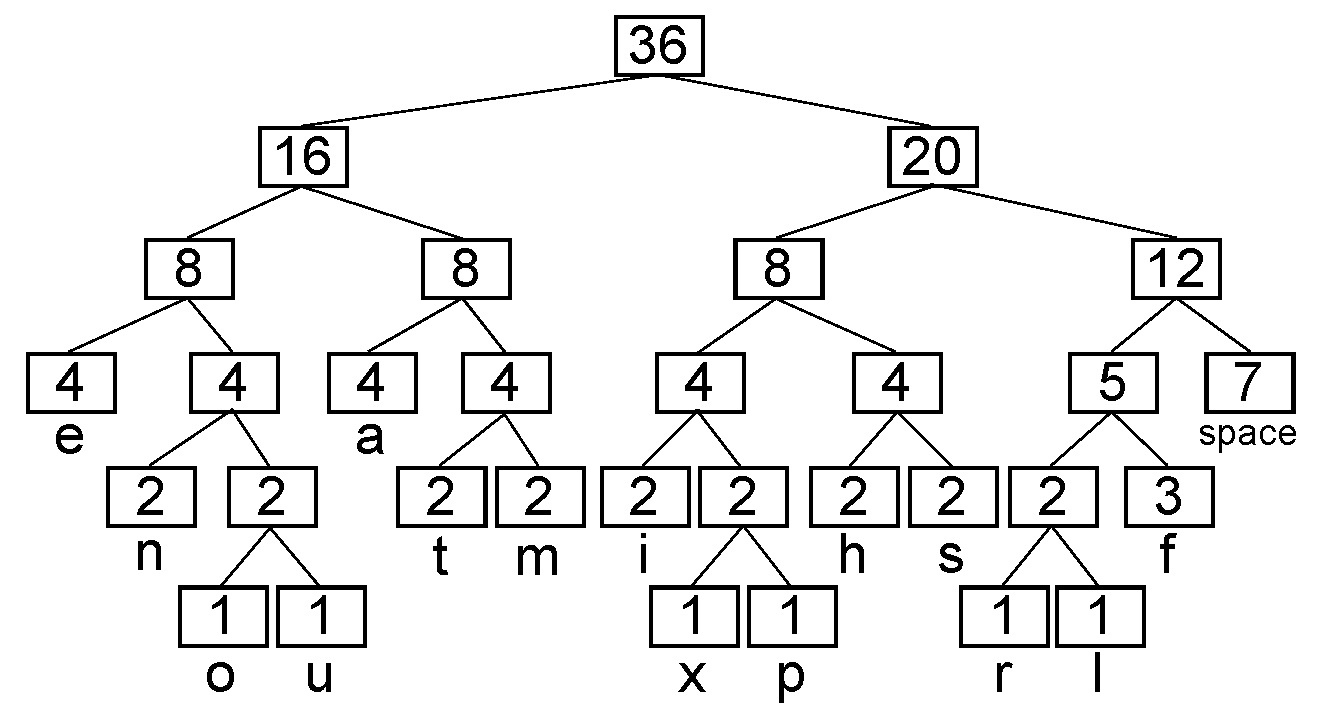
\includegraphics[scale=0.5]{figs/related_work/huffman.pdf}
    \caption{Visualisation of an example Huffman tree, created with the string "this is an example of a huffman tree" as input. Source: \citet{Dcoetzee2007}}
    \label{fig:huffman}
\end{figure}
%https://commons.wikimedia.org/wiki/File:Huffman_tree.svg

\begin{table}[h!]
\begin{tabular}{|lll||lll||lll|}
\hline
\textbf{Char} & \textbf{Freq} & \textbf{Code} & \textbf{Char} & \textbf{Freq} & \textbf{Code} & \textbf{Char} & \textbf{Freq} & \textbf{Code} \\ \hline
space         & 7             & 111           & m             & 2             & 0111          & p             & 1             & 10011         \\
a             & 4             & 010           & n             & 2             & 0010          & r             & 1             & 11000         \\
e             & 4             & 000           & s             & 2             & 1011          & u             & 1             & 00111         \\
f             & 3             & 1101          & t             & 2             & 0110          & x             & 1             & 10010         \\
h             & 2             & 1010          & l             & 1             & 11001         &               &               &               \\
i             & 2             & 1000          & o             & 1             & 00110         &               &               &               \\ \hline
\end{tabular}
\caption{Table that accompanies Figure~\ref{fig:huffman}. It contains all characters of the original string with their frequencies and the binary code with which they are mapped. Source: \citet{Dcoetzee2007}}
\label{tab:huff}
\end{table}


% Add something about performance, decoding and how strings are actually coded

\subsection{DEFLATE and zlib}
\label{sec:zlib}
Zlib is a free general purpose compression library that uses the Deflate method, which in turn is based on Huffman coding and \ac{lz77} compression.
The input data is split into a series of blocks.
Each block is compressed separately by using \ac{lz77}.
Subsequently, Huffman coding is used on the encoded blocks.
For the latter part, zlib has two different implementations that are performed on individual blocks: either with creation Huffman trees with the algorithm which is then stored alongside the data, or by using default trees that are defined in DEFLATE which removes the need of storing the extra information \citep{zlib}.

\subsection{Smaz}
\label{sec:smaz}
Even though it can be used on any kind of natural language text, Smaz is a compression library for the specific purpose of working well on small strings.
General purpose compression techniques tend to have a larger overhead in order to be able to work well with dynamic input, which is why Smaz is potentially more suitable for this specific case \citep{antirez}.
It works with a static codebook containing frequent-occurring English (fragments of) words and bigrams. 
This makes it likely to work best on English strings, however, this is subject to testing.
The parts are encoded in binary, with the most frequent parts being in the smallest representation \citep{antirez2}.
Its general idea is thus similar to Huffman coding (see \ref{sec:huffman}).

%\subsection{tar + gzip}
%This is used by Cesium (or at least in their tests), could be worth investigating.


\section{Compression of geometries, meshes, and graphs}
\subsection{Quantisation}
\label{theoryquantisation}

Quantisation is a technique that can be regarded as lossy compression.
It is used for signal processing, converting continuous data from an analogue source to a digital representation.
But it can also be applied to data that is already digitalised, for instance a list of coordinates as is exemplified by Draco in this thesis.
It works by mapping a dictionary containing all values that the data encompasses to a dictionary reduced in size, to which original values are joined many-to-one.
This means for example that a value that occurs once will be mapped to a value that is close to it but occurs more frequently, losing some of the original information \citep{sayood2017introduction}.
Vector quantisation can be used to compress coordinates \citep{rossignac20013d}.


\subsection{Delta encoding}
Another used name for this concept is delta compression.
It is for instance used for version control, the distribution of software patches, and other transmission of data over the web.
The idea behind it is to only store or transmit the delta (difference) of the data to data that is already stored or received.
The complete data can subsequently be reconstructed by adding the delta to the existing data that it is connected to \citep{suel2019delta}.
The technique can be applied within a complete set of data as well as is is for example done in \citet{deering1995geometry}, where vertices are stored in an array as a vector of the delta difference with the previous vertex.
Both transmitting deltas and storing deltas in a complete dataset are relevant for this thesis in the context of streaming and the compression of geometry as well as feature attributes.




\subsection{Edgebreaker}
\label{sec:theoryedgebreaker}

Edgebreaker is one of the techniques used by Draco to compress 3D triangle meshes.
A mesh that consists of triangles can be represented by the vertex data, which is made up of the coordinates of all vertices that the mesh encompasses, and the connectivity, which defines the relation between the triangles (or faces) and the vertices that belong to it.
This is how Wavefront OBJ files are structured as well, which is followed by CityJSON.
The Edgebreaker algorithm compresses the connectivity data of meshes \citep{rossignac2003edgebreaker}.\\

%This upper-bound on storage does not rely on statistic-based entropy or arithmetic coding schemes, which in general perform poorly on small or irregular meshes. Consequently, Edgebreaker is particularly attractive for compressing large catalogs of small models.
% van edgebreaker on a corner

\subsubsection{Compression}
To encode this information, first a spiraling triangle spanning tree is created for the mesh \citep{rossignac2003edgebreaker}. Analogised with peeling an orange, it is done by cutting around the peel in a spiraling way, after which it can be laid out flat.
This is visualised in Figure~\ref{fig:spanningtree}.
With a mesh this would result into a curled string of triangles.
Ultimately, the dual graph of this string represents the spanning tree \citep{taubin1998geometry}.\\

\begin{figure}[h]
    \centering
    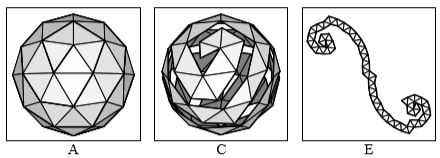
\includegraphics[scale=0.8]{figs/related_work/spanningtree.jpg}
    \caption{Visualisation of the creation of a triangle spanning tree, not showing the dual graph representation. Figure taken from \citet{taubin1998geometry}}
    \label{fig:spanningtree}
\end{figure}

% https://www.sciencedirect.com/topics/computer-science/spanning-tree
% en corner-table paper
Consequently, the algorithm traverses the triangles of the spanning tree, keeping track of all visited triangles and the vertices they are bounded by.
Each triangle is assigned one character of the set \texttt{\{C,L,E,R,S\}}, which denotes one of the five cases (see Figure~\ref{fig:clers}) that are defined in the specification of the algorithm.
C means that the shared vertex v, between the current triangle and the ones to its left and right, has not been visited at all.
As for the other four cases, vertex v has been visited and the triangle left or right (L or R), both of them (E) or neither of them (S) has been traversed \citep{rossignac2003edgebreaker, rossignac20013d}.


\begin{figure}[h!]
    \centering
    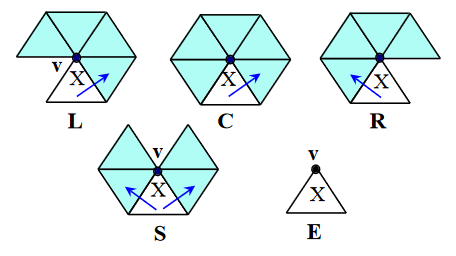
\includegraphics[scale=0.8]{figs/related_work/clers.png}
    \caption{The five cases defined for the Edgebreaker method. X is the current triangle in the iteration, v the vertex that is shared between X and the triangles to its left and right, and blue triangles are unvisited. Figure taken from \citet{rossignac2003edgebreaker}}
    \label{fig:clers}
\end{figure}

During the traversion of the triangles two tables (M and U) are created to respectively store the visited vertices and triangles, and two others (V and O) are used to keep references to vertices and their opposite corners.

Optionally, a prediction method for \texttt{CLERS} symbols of succeeding unencoded triangles can be used, which is based on the vertex valences \citep{dracopredictive}.
The valency (or degree) of a vertex is the amount of edges that is emanating from it.
The addition of this method can decrease the file size in similar fashion to parallelogram prediction (see Section~\ref{sec:parallelogram}), as symbols would not have to be stored explicitly.

%https://github.com/google/draco/blob/master/src/draco/compression/mesh/mesh_edgebreaker_traversal_predictive_encoder.h
%// Encoder that tries to predict the edgebreaker traversal symbols based on the
%// vertex valences of the unencoded portion of the mesh. The current prediction
%// scheme assumes that each vertex has valence 6 which can be used to predict
%// the symbol preceding the one that is currently encoded. Predictions are
%// encoded using an arithmetic coding which can lead to less than 1 bit per
%// triangle encoding for highly regular meshes.

\subsubsection{Decompression}
Decompressing the mesh the V (vertice references) and O (opposite corners references) tables will be reconstituted, and after that the table containing the vertex positions.
The \texttt{CLERS} string is iteratively decoded to create a triangulated polygon that approaches C in Figure~\ref{fig:spanningtree}, adding one triangle at a time. 
An S triangle will invoke the start of the decompression of one string of triangles (as there are multiple ones because of recursive compression).
Encountering an E means that the end of the string is reached in the current recursion iteration.
Depending on the other symbols that are encountered, the bounding edges shown in C in Figure~\ref{fig:spanningtree} are zipped up by matching pairs of edges.
In this way, ultimately shape A in Figure~\ref{fig:spanningtree} is reconstituted.
After the decompression of the connectivity information, the positions of the vertices are decompressed \citep{rossignac2003edgebreaker}.
%An S triangle will invoke the start of the decompression of one string of triangles (as there are multiple ones because of recursive compression).
%If a C is encoutered, this means that no adjacent triangles have been decoded yet, as according to the CLERS string they were not visited at that point. 
%Therefore, no zipping of edges takes place yet.
%Only when an L is encountered, meaning that its left triangle has been visited, will a zip take place between the left edge of L and the adjacent edge of the previously visited C triangle.
%As for an R triangle, its opposite edge is labeled with -2, but no zipping is attempted. That edge is zipped later in another recursion iteration.
%Encountering an E means that the end of the string is reached in the current recursion iteration.
%This means that all free edges can be zipped, as long as the one on the right is marked with -2 and the one on the left with -1.
%It is then when R triangles are zipped as well.



%For this purpose a so-called Corner-Table, consisting of two arrays of integers, is created which describes the connectivity information.



% edgebreaker vs andere oudere algoritmes? was een paper over



\subsection{Sequential connectivity compression}
\label{sec:seqconnectivity}

An alternative method to edgebreaker that Draco can use is their own sequential connectivity method.
It either uses delta encoding (storing the difference of vertex coordinates to the ones of the previous vertex \citep{deering1995geometry} to store the IDs of vertices after which they are compressed by entropy encoding (of which Huffman coding is an example---~\ref{sec:huffman}), or the IDs are simply stored using everytime the amount of bits that the largest vertex id takes up \citep{Google2019}.
In contrast with edgebreaker, this method preserves the vertex order within triangles.
% (does it also preserve face order?) i could test myself
On the other hand the resulting encoding will not be as small.

%https://github.com/google/draco/issues/132
%It also does not use "some of the more advanced algorithms for point attribute compression (such as parallelogram prediction, etc..). This may change in future if there is demand for it.".

\subsection{Parallelogram prediction}
\label{sec:parallelogram}
Parallelogram prediction compresses meshes by predicting the missing vertex of a triangle, knowing the two vertices from the edge shared with a previously decoded triangle \citep{gotsman-touma-gi98, Google2018}.
A basic prediction can be made with the so-called parallelogram rule, as defined by formula~\ref{eq:parallelogram}, with the variables referring to the vertices in Figure~\ref{fig:parallelogram}.

\begin{equation}
r^p = v + w - u
\label{eq:parallelogram}
\end{equation}

However, this prediction can be improved by taking an estimated crease angle between the two triangles (the "crease" being the shared edge---the angles are depicted on Figure~\ref{fig:parallelogram} with the lines crossing edges (\(s,v\)) and (\(v,u\))) into account, as opposed to assuming that they are co-planar.
This angle is estimated based on at least one set of adjacent triangles, that thus has to be decoded already.
If there are more adjacent triangles available, it is taken as the average of the crease angles between the two sets of triangles that are closest to parallel to the shared edge of the current triangle and the predicted one \citep{gotsman-touma-gi98}.
As example, \(r_ca^p \) on Figure~\ref{fig:parallelogram} is the predicted vertex of the next triangle by taking the crease angles between triangles (\(s,v,t\)) and (\(s,v,w\)).

Ultimately, the mesh is compressed by storing the error of the predicted vertex to the actual vertex (as a vector) rather than the vertex itself. 
It is therefore a completely lossless technique.

\begin{figure}[h!]
    \centering
    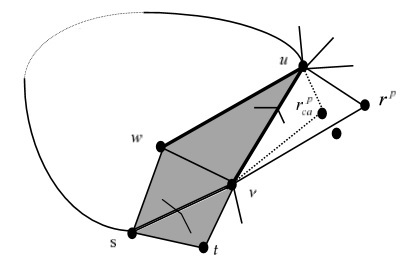
\includegraphics[scale=0.8]{figs/related_work/parallelogram_rule.jpg}
    \caption{Illustrated how a new vertex can be predicted using parallelogram prediction. \(r^p\) is the vertex as predicted with the parallelogram rule, \(r_ca^p \) is as predicted with the crease angle taken into account. Figure adapted from \citet{gotsman-touma-gi98}}
    \label{fig:parallelogram}
\end{figure}




%\subsection{Entropy encoding}
%Huffman is one of the most common forms of entropy encoding (according to wikipedia at least).
%\citep{mackay2003information}


%\subsection{Sequential connectivity}
%This is the second method that Draco can use, but of which I could not find proper information yet.

%\subsection{Streaming meshes}
%The algorithm from the Isenburg paper.
%!TEX root = thesis.tex
\chapter{Related work}
\label{chap:rw}

\section{CityJSON}
\label{sec:cityjsonexplained}

CityJSON \citep{cityjsonspecs} is an encoding for storing digital twins, containing geometries and attributes of real world features such as buildings, terrains, roads, and waterbodies.
It is based on the data model of CityGML \citep{citygml}, but uses \ac{json} as encoding for it rather than \ac{gml} which poses advantages in file compactness and ease of use.
The file format has four main characteristics that can be exploited for compression purposes: the \ac{json} encoding, geometries, attributes, and textures.
As mentioned in Section~\ref{sec:datacompression}, prior knowledge on the input data allows for more suitable compression techniques to be chosen.
Furthermore, the explanation helps in understanding the difference with other file formats that are introduced in Sections~\ref{sec:b3dm} and~\ref{sec:i3s}.

The \ac{json} format is easy for humans to read, while at the same time relatively lightweight (in comparison to for example \ac{gml}) \citep{json}.
In its specification several data types are defined: boolean values, numbers, strings, arrays (ordered lists of elements), and objects (containing key-value pairs).
These data types can be combined and nested \citep{ledoux2019cityjson}.
In Listing~\ref{ls:cj2} it is shown how this looks like with example snippet of a CityJSON dataset.
However, the readability comes at the cost of verbosity.
This is exemplified by the binary JSON-like format \ac{cbor} which is introduced in Section~\ref{sec:cbor}.

A CityJSON file is a \ac{json} object contains 4 mandatory keys:
\begin{enumerate}
\item \texttt{"type"} (which is always of value \texttt{"CityJSON"})
\item \texttt{"version"}
\item \texttt{"CityObjects"} (a \ac{json} object containing objects that represent geographical features)
\item \texttt{"vertices"} (an array containing the coordinates of all vertices)
\end{enumerate}

A feature in CityJSON is called a city object and can be of a variety of types (shown in Table~\ref{tab:cityobjects}) as derived from CityGML's data model \citep{ledoux2019cityjson}.
A city object is not limited to these types, as extensions can add others.
A 2nd-level city object can be a child of a 1st-level city object parent, and thus linked together in this way.





It always has a \texttt{"geometry"} key which is an array containing more than 0 geometry objects, which can represent several \ac{lod}s.
A geometry object in turn can be of several types of 3D geometric primitives.
The vertex coordinates of a 3D model are stored in one array as shown in the above list, but the connectivity information is stored in geometry objects.
Here, references to vertices are stored.
This is inspired on the Wavefront OBJ \citep{Reddy} format, and these parts are depicted in the green in listings~\ref{ls:cj2}, and ~\ref{ls:cj3}.
Optionally, a city object can have an "attributes" object as member.
Here all attributes can be stored as defined in CityGML's data model, with which extension is possible as well \citep{ledoux2019cityjson, cityjsonspecs}.

%These elements are marked with the red rectangles in listings~\ref{ls:cj1} and ~\ref{ls:cj2}.

In addition, there are optional keys for extensions, metadata, coordinate transform, appearance, and geometry-templates. 
Metadata can contain for example the geographical extent of the data, and coordinate transform gives the option to define a coordinate offset, which enables compression through the conversion of coordinates to integers and moving the origin to (0, 0, 0) \citep{ledoux2019cityjson, cityjsonspecs}.
This actually is a form of quantisation (Section~\ref{theoryquantisation}).
The basic structure of a CityJSON file is shown in listing~\ref{ls:cj1}, including \texttt{"metadata"} and \texttt{"transform"}.

Lastly, it can contain materials, textures, and semantic surfaces belonging to city objects.
These are respectively stored following the X3D specifications and with additional COLLADA files \citep{ledoux2019cityjson, cityjsonspecs}.
This is however out of the thesis scope (see~\ref{sec:scope}).

\begin{table}
 \begin{tabular}{ |l|l| } 
 \hline
  1st-level city objects & 2nd-level city objects\\
 \hline \hline
      \multirow{2}{45mm}{Building}&BuildingPart\\
    &BuildingInstallation\\
\hline
      \multirow{3}{45mm}{Bridge}&BridgePart\\
    &BridgeInstallation\\
    &BridgeConstructionElement\\
\hline
\multirow{10}{45mm}{CityObjectGroup\\CityFurniture\\GenericCityObject\\LandUse\\PlantCover\\Railway\\Road\\SolitaryVegetationObject\\TINRelief\\TransportSquare} 
      &\\
      & \\
      & \\
      &\\
      & \\
      &\\
      & \\
      & \\
      &\\
      & \\
\hline
      \multirow{2}{45mm}{Tunnel}&TunnelPart\\
    &TunnelInstallation\\
\hline
WaterBody & \\
\hline
\end{tabular}
\caption{Types of city objects (features) that CityJSON natively supports (from \citet{ledoux2019cityjson}}
\label{tab:cityobjects}
\end{table}

\clearpage

\begin{scriptsize}
\hspace{-1.6cm}\begin{minipage}[c]{0.45\linewidth}

\lstdefinestyle{base}{
backgroundcolor=\color{lichtgrijs}, 
  moredelim=**[is][\color{orange}]{@}{@},
}

\begin{lstlisting}[frame=single,style=base,caption={Snippet of CityJSON structure, with mandatory members in orange}, label=ls:cj1]
{
    @"type": "CityJSON",@	
    @"version": "1.0",@	
    @"CityObjects": {..},@	
    @"vertices": {..},@	
    "metadata": {
        "geographicalExtent": [	
            84616.468,	
            447422.999,	
            -0.47,	
            85140.839,	
            447750.636,	
            13.8	
            ],	
        "referenceSystem": "urn:ogc:def:crs:EPSG::7415"	
        },	
    "transform": {	
        "scale": [	
            0.001,	
            0.001,	
            0.001	
            ].	
        "translate": [	
            84616.468,	
            447422.999,	
            -0.47		
    }
}
\end{lstlisting}


\end{minipage}
\hspace{0.2cm}
\begin{minipage}[c]{0.42\linewidth}

\lstdefinestyle{base}{
backgroundcolor=\color{lichtgrijs}, 
  emptylines=1,
  breaklines=true,
basicstyle=\ttfamily\color{black},
  moredelim=**[is][\color{orange}]{@}{@},
moredelim=**[is][\color{Green}]{|}{|},
}

\begin{lstlisting}[frame=single,style=base,caption={Snippet of basic structure of CityObjects. Attributes in orange, geometries in green}, label=ls:cj2]
{
    "type": "CityJSON",
    "version": "1.0",
     "CityObjects": {
        "b0a8da4cc-2d2a-11e6-9a38": {
            @"type": "BuildingPart",@	
            @"attributes": {@	
            @"creationdate": "2014-07-09",@	
                @"terminationdate": "",@	
                @"function": "garage"@	
                @},@	
                |"geometry": [|	
                |{|	
                    |"type": "Solid",|	
                    |"boundaries": [|	
                        |[|	
                            |[|	
                                |[|	
                                    |[0, 1, 2],|	
                                    |[1, 2, 3],|	
                                    |[1, 3, 4],|	
                                    |[0, 1, 4]|	
                                |]|	
                            |]|	
                        |]]|	
                    |},|	
                    |"lod": 2,|	
                |},|	
            "parents": ["b0a8da4cc-2d2a-11e6-9a39"]
            },
        "b1105d28c-00ba-11e6-b420": {..},
        "b1126a169-00ba-11e6-b420" {..}
    },
    |"vertices": [..]|
}
\end{lstlisting}


\end{minipage}
\hspace{0.2cm}
\begin{minipage}[c]{0.30\linewidth}

\begin{lstlisting}[frame=single,style=base,caption={Snippet of vertex array of CityJSON, highlighted in green}, label=ls:cj3]
{
    "type": "CityJSON",
    "version": "1.0",
    "metadata": {..},
    "CityObjects": {..},
     |"vertices": [|	
          |85012.343,|	
          |447455.577,|	
          |-0.27|	
          |],|	
          |[|	
          |85010.804,|	
          |447448.808,|	
          |-0.27|	
          |],|	
          |[|	
          |85013.832,|	
          |447447.447,|
          |-0.27|	
          |],|	
          ...
}
\end{lstlisting}

\end{minipage}
\end{scriptsize}


\section{Draco}
\label{rwdraco}

Draco, an open-source library by Google for compression and decompression of geometric meshes \citep{draco}, can be used to compress the geometrical part of the CityJSON structure.
Generally, it works with the Edgebreaker algorithm (which is explained in Section~\ref{sec:theoryedgebreaker}), their own sequential connectivity method (Subsection~\ref{sec:seqconnectivity}), parallelogram prediction (Subsection~\ref{sec:parallelogram}), and the quantisation of coordinates (Subsection~\ref{theoryquantisation}).
It can compress both 3D geometrical meshes and point clouds, but only the former is relevant for this application.
On average, it compresses meshes (that are in Wavefront OBJ format) to about 2 percent of their original file size \citep{dracoperformance}.
It has encoders and decoders written in C++ and JavaScript (and exclusively a decoder in WebAssembly), enabling it to be suitable for both offline (in this case preparation of compressed CityJSON files) and online (decoding the compressed geometries in the browser) purposes.\\

Not just the savings on file storage itself are beneficial, but since files are transferred over the web for browser use, time is saved as the data is in a slimmer format.
The network speed can form a bottleneck, and it is exemplified by Cesium that using Draco can potentially improve the rendering speed as it is decoded asynchronously, meaning that parts are already rendered while the complete dataset is still being downloaded \citep{cesiumdraco}.


There are three main configurations that can be set when encoding a mesh.
First, there is the compression level parameter which goes from 0 to 10.
Based on this parameter, different compression features that the library encompasses are used, with 10 giving the most compressed result but at the same time having the worst decompression time.
Second, a parameter that specifies the amount of bits to which the input values should be quantised can be chosen (which would make the compression lossy if used---see Section~\ref{theoryquantisation}), and lastly, there is the option to retain the separation between objects \cite{dracoperformance}.


Draco compressed meshes are stored in their native .drc binary format.
The format generally consists of four parts: a header, metadata (object id for example), connectivity data, and attributes, as shown on Figure~\ref{fig:draco_format}.


\begin{figure}[h!]
    \centering
    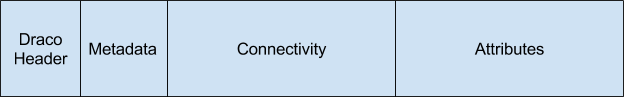
\includegraphics[scale=0.5]{figs/related_work/draco_format.png}
    \caption{The general structure of the Draco file format (.drc). Figure taken from \citet{dracospec}}
    \label{fig:draco_format}
\end{figure}


%\section{Text compression}
%Besides the geometry of CityJSON files, its semantics that are repesented as text can be compressed as well. 

\section{glTF}
\label{sec:gltf}
\ac{gltf} is a file format that is designed for efficient loading of 3D graphics and their dissemination over the internet \citep{KhronosGroup2019}. 
It is formatted in \ac{json} and keeps file sizes small, can be processed fastly and is an extensible format.
The elements that it contains conceptually have a hierarchical relationship as shown in Figure~\ref{fig:gltf}.
Roughly explained, a scene is one model, and a file can contain multiple ones.
A scene in turn contains nodes (which are features---for example a building).
These do not have a specified \ac{crs}, but can have their own translation, rotation, and scale properties, similar to CityJSON's \texttt{"transform"} (see Section~\ref{sec:cityjsonexplained}.
Their geometries are stored in a combination of meshes, buffers, bufferViews, and accessors, and it is possible to include skins, animations, cameras, materials, and textures.
Moreover, it is possible to include for example buffer geometries and textures in binary format.

\begin{figure}[h!]
    \centering
    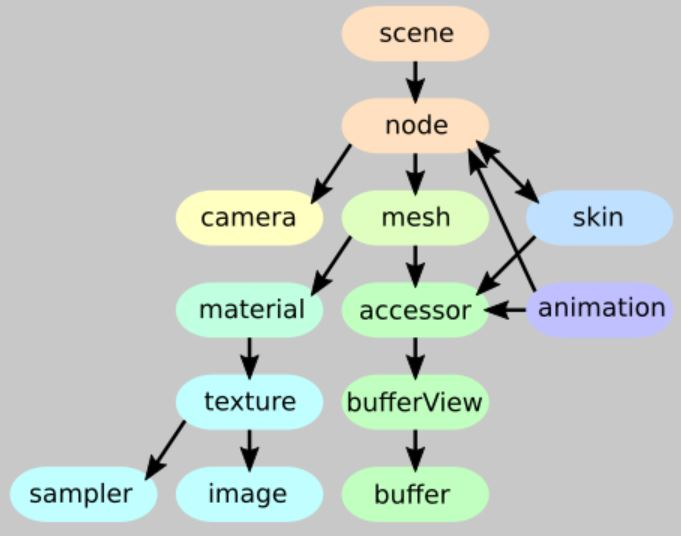
\includegraphics[scale=0.5]{figs/related_work/gltf.jpg}
    \caption{The conceptual structure of the \ac{gltf} format (cropped from \citet{KhronosGroup2019})}
    \label{fig:gltf}
\end{figure}

\section{Cesium 3D Tiles}
\label{sec:3dtiles}
Despite this part being out of scope for this thesis (as stated in the introduction), it is still important to notice its existence as it can make a contribution to the efficient streaming of 3D geoinformation.
Besides that, it is implemented by the \ac{b3dm} format (see Section~\ref{sec:b3dm}), which is an alternative to CityJSON for web visualisation.

Created for the sharing, visualisation, and analysis of 3D geoinformation, the 3D Tiles specification \citep{3dtiles} is a \ac{json} object in which the data is separated into tiles.
Every tile is described by a bounding volume and the tiles are organised into a tree, which could be a quadtree, octree, k-d tree, or grid.
Tiles can have children, creating a hierarchical structure with which different LoD can be represented.
The tile parent would contain the 3D model in a low LoD, and every child would contain either more details that can be rendered when needed, or again a full 3D model but with a higher LoD \citep{Cesium2020}.

Its implementation can thus benefit the streaming of massive datasets as it allows the loading of smaller parts (tiles) as they are needed, e.g. when they are zoomed into, and in the LoD that they are wanted.
In Section~\ref{sec:b3dm} an implementation of 3D Tiles is explained, giving more details about the structure.


\subsection{Batched 3D Model}
\label{sec:b3dm}
b3dm is a binary file format that can store heterogeneous 3D models and incorporates the 3D Tiles specification \citep{b3dm}.
It roughly consists of three parts: a feature table, batch table, and \ac{gltf} geometry.
In the specification a feature is a 3D model and the feature table can thus be seen as a collection of tiles.
Every feature may have a position property indicating the coordinates of its centre.

In the batch table the properties of the contents of features are contained.
These properties are stored in \ac{json} format, but in a different fashion than CityJSON's CityObjects. 
It is an array value with the name of the property as key, with the array containing values for the ordered objects of the feature.
This means that if there is an n amount of objects, the array for a property will contain n elements.
An example is as follows:

\blockquote{"height" : [10.0, 20.0, 15.0]}

Alternatively, the properties can be stored in a binary body to which a reference is placed within the aforementioned JSON structure.
Since this way of storing attributes is inefficient when there are properties that only apply to a subset of objects (for example "amount of leafs" for trees, which buildings would not have), it is possible to define object types which have their own set of property names.

Lastly, the geometries of the objects from all features are stored as \ac{gltf}, which allows for the use of Draco compression as well since it can be embedded therein.

The format therefore is similar to the aimed end-result of this thesis, with the additional benefit of having the option to structure the data into tiles.
On the contrary, it lacks the benefits of the CityGML data structure, the tools that exist for CityJSON, and (further) compression of attributes \citep{b3dm}.

\section{Esri I3S}
\label{sec:i3s}
\ac{i3s} \citep{i3sspecsmain} is an open file format by Esri.
The scene layer that it encodes in turn contains large volume heterogeneous geographic data (\eg\ 3D objects, point clouds, and buildings). 
It is formatted in JSON and specifically designed for the efficient streaming of massive 3D datasets. 
Similarly to CityJSON, Scene Layers encompass the geometry, texture, and attributes of features. 
Features are grouped into nodes with the nodes forming a regular or irregular tree by their bounding sphere (or oriented bounding box), akin to respectively a quadtree or an R-tree.
Parent nodes in a tree contain the features with a lower LoD.
Because of this structure, specific nodes can be found faster and loaded more efficiently as well as simpler representations of geometries can be shown when they are looked at from afar \citep{i3sspecs, i3sspecsmain}.

A node in itself does not contain complete features, but rather IDs which point to geometry buffers (encoded with Draco), textures, and attributes.
The standard allows any geodetic coordinate reference system to be used, with the node having the same \ac{crs} as the vertices that it encompasses.
The vertex position are stored with the centre of the node's bounding area as offset, allowing for compression and easier visualisation in for example three.js.
LoD are not the same in I3S as in CityJSON---it uses thinning, clustering, and generalisation of 3D objects or meshes, as well as the downsampling of textures.
The to-be visualised LoD (thus which leaf of the tree is chosen by the viewer) is determined by screen size, resolution, bandwith, and memory \citep{i3sspecsmain, i3sspecs}.




\section{Binary JSON}
Binary file formats can be more concise and processed (reading or writing) faster, as explained in Section~\ref{sec:binary}.
It is therefore relevant for the improvement of CityJSON's efficiency.
Additionally, it can be beneficial to store binary data in JSON format, such as encryption keys or graphics like Draco geometries (see~\ref{rwdraco}).
JSON natively does not allow for this and requires such data to be encoded in Base64 format.
This is a family of binary-to-text encoding schemes that is utilised when binary data needs to be stored, while working with media that are created to handle ASCII rather than binary data \citep{cborurl}.
The downside of this is that a string in Base64 encoding can be 33\% larger than its binary form \citep{Mozilla2020}.

There are several different binary formats that encode data in a JSON-like manner.
In a \ac{json} library for C++ by \citet{nlohmann}, the following ones are implemented: \ac{bson}, MessagePack, \ac{ubjson}, and \ac{cbor}.
I have chosen to use \ac{cbor} for the reasons below, as derived from a comparison with \ac{cbor} from \citet{cborspecs}, but this does not necessarily mean it is the best-performing option for the use cases of this thesis.
\ac{bson} is specifically developed for MongoDB \citep{MongoDB2020}.
This means that it is adapted for that purpose and this could make it less efficient for other purposes.
It does have the possibility for updating values, but this comes at the cost of less concise storage.
MessagePack is similar to \ac{cbor}, but has caveats that have to do with backwards compatibility and there is not much space for extension of the specification anymore.
\ac{ubjson} exactly mimics the \ac{json} data model, which means that it can not store binary values.
However, this functionality is necessary for storing Draco geometries within a CityJSON-like (compressed) file.





\subsection{CBOR}
\label{sec:cbor}
\ac{cbor} has two clear purposes that were stated prior to its development, which are storing binary strings into a JSON-like format and compression of data \citep{cborurl}.
Like \ac{json}, it follows a key-value structure. 
Roughly explained, every data item starts with an initial byte the contains information about the major type of the item and supplementary information.
The major type can be one of the following \citep{cborspecs}:
\begin{itemize}
\item Unsigned integer
\item Negative integer
\item Byte string
\item Text string
\item Array
\item Map (JSON-style object)
\item Optional semantic tagging of other types (such as date/time string, URI, base64)
\item Floating-point number
\end{itemize}

When reading the data, knowing the type and length of a value increases the performance as mentioned in Section~\ref{sec:binary}.

%!TEX root = thesis.tex
\chapter{Methodology}
\label{ch:meth}


The network speed is always a bottleneck when transmitting complete CityJSON datasets over the web and doing something with the data, as the receiver can only do something with it once the data has arrived.
The assumption we thus make is that compressed datasets will have a better performance when the time that is gained in network transmission speed is larger than the time that is lost decoding the data after arrival.
This Chapter lays out the plan to benchmark the performance of several types of compressed CityJSON compared to uncompressed CityJSON, to find the advantages and disadvantage of techniques and give recommendations on what the best compression types would be given specific scenarios.

Shown in Figure~\ref{fig:workflow} is the structure of the methodology, divided into four general parts:
\begin{itemize}
\item The implementation of compression techniques for CityJSON
\item The preparation of datasets to test compression techniques with
\item Preparation of a testing platform that can work with both uncompressed and compressed CityJSON files
\item Testing and benchmarking the performance of different file types on the performance indicators of Table~\ref{tab:methindicators}, which were introduced in Section~\ref{sec:researchq}
\end{itemize}

The first three are finished prior to the benchmarking, in order to avoid having to redo work for part 2 when something had been changed in part 1.
The tasks in part 1 are grouped together because there is no necessary order and are implemented simultaneously.
All four are explained further in the next sections.

\begin{figure}[h!]
    \centering
    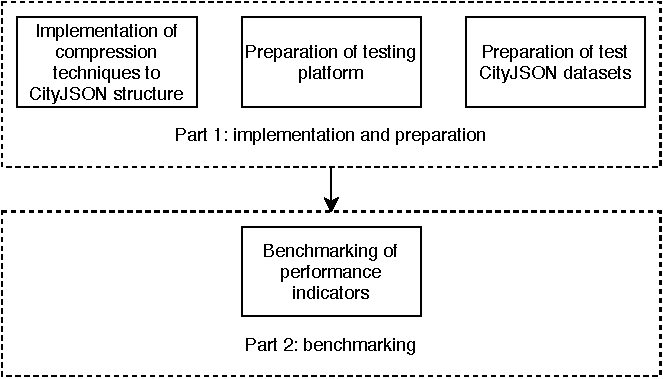
\includegraphics[scale=1]{figs/methodology/methodology_flow2.pdf}
    \caption{The general research workflow}
    \label{fig:workflow}
\end{figure}

\begin{table}[h!]
\begin{center}
 \begin{tabular}{ |c |} 
 \hline
  Compression type performance indicators \\ [0.5ex] 
 \hline\hline
 Visualisation time \\
 \hline
 Querying time \\
 \hline
 Spatial analysis time \\
 \hline
 Editing time \\
 \hline
 File size compression \\ 
 \hline
 Lossiness \\
 \hline
\end{tabular}
\caption{The six performance indicators on which variants of compressed CityJSON are assessed}
\label{tab:methindicators}
\end{center}
\end{table}




\section{Implementation of compression techniques}
\label{sec:compressionimplementation}

In Chapter~\ref{ch:theory} a multitude of compression techniques has been introduced.
Different combinations of these techniques are applied to the CityJSON structure and be compared on the six defined performance indicators (see Table~\ref{tab:methindicators}), with the performance of uncompressed CityJSON as the baseline.
A possible outcome is that certain combinations of techniques are more suitable for specific purposes, making it difficult to choose one that is the best.
Chapter~\ref{ch:bmresults} shows which compression types 
For this reason, there is a depthly discussion about it in Chapter~\ref{ch:bmresults}.

Table~\ref{tab:compressionmethods} shows which combinations of compression techniques I implement on CityJSON and benchmark on time performance.
The table has a divide between compression methods where the geometries are kept as is, and where they have been replaced by Draco-compressed geometry.
All other names besides "original" and "draco" indicate either the inclusion of a binary format or a compression technique.

The only compression technique that has not been explained in Chapter~\ref{ch:theory} is the so-called replace technique, which I have created.
It means that all keys and values of "CityObjects" from the \ac{json} structure are copied to a separate array.
The elements of the array are sorted by frequency, and the keys and values in the \ac{json} are replaced with a reference to the array.
This has three supposed advantages: 

\begin{enumerate}
\item The \ac{json} structure is retained, of which parts could be reconstituted as wanted. It would for instance be possible to only decode the first City Object rather than all of them. When using a compression technique directly on the \ac{json} structure, all data has to be decoded prior to use.
\item The array allows for greater compression as the keys and values can be compressed at once with for example zlib, as opposed to compressing all of them individually.
\item Redundancy is removed, as keys and values that appear more than once are only stored as one array element.
\end{enumerate}
The array can be stored as a member of the CityJSON object and thus optionally be included in a \ac{cbor} representation.
An example of how a dataset compressed in this way looks like is found in Section~\ref{sec:implreplace}.


Ultimately there are 20 different types of CityJSON tested, of which 19 are compressed variants and 1 is original CityJSON.
However, "original CityJSON" is defined as including the "transform" member (as stated in Section~\ref{sec:researchq}, with "transform" being explained in Section~\ref{sec:cityjsonexplained}), which is done for the uniformity of datasets and because Draco needs coordinates to be stored in this manner before compression.
It is however already a form of compression, but included in the CityJSON specification \citep{cityjsonspecs}.



They tested CityJSON types are divided into two categories: having geometry compressed by Draco, or geometry as originally implemented in CityJSON.
So there are actually 10 pairs, within which the difference is the use of Draco.
Table~\ref{tab:compressionmethods} shows all CityJSON implementations, and in the following enumeration a brief description is given for all 10 combinations:

\begin{enumerate}
\item The dataset is in the style of regular CityJSON, but needs to include "transform". "original" is the baseline to which all other combinations are compared. 
As for "draco", the Draco \ac{blob} is placed underneath the \ac{json} structure, with a delimiter inbetween. 
It can not be added as a member of the CityJSON object as \ac{json} does not allow binary values.
This means that the result is a binary file.
\item The same as 1, but with the complete file compressed with zlib (see Section~\ref{sec:zlib}).
\item Similar to 1, but with the CityJSON object parsed into \ac{cbor} (see Section~\ref{sec:cbor}). 
In this case, the Draco \ac{blob} is added as a member of the CityJSON object as it does allow for binary values.
This would make it easier and quicker to read as well, since the file does not need to be split by a delimiter.
\item Encoded in \ac{cbor} like 3, but all keys and string values of the CityJSON object are compressed by smaz.
This only works in combination with cbor, because strings are binary-encoded by smaz.
\item Same as 3, but with the resulting \ac{cbor} (Section~\ref{sec:cbor}) compressed with zlib (Subsection~\ref{sec:zlib}).
\item Similar to 1, but with all keys and values copied to an array and replaced by references.
\item Same as 6, but with the array  compressed with zlib.
\item Same as 6, but with the CityJSON object parsed into \ac{cbor}.
\item Same as 8, but with the array compresed with zlib.
\item Same as 8, but with the array compressed with Huffman coding (see Section~\ref{sec:huffman}).
\end{enumerate}


%For compression combinations using Draco, the array of vertices and all the boundaries of Geometry Objects are stripped from the dataset.
%The geometries are compressed by Draco and stored in the file as a \ac{blob}.


\begin{table}[]
\begin{tabular}{|l||l|l|}
\hline
 & \textbf{Original geometry}    & \textbf{Draco geometry}    \\
\hline \hline
1 & original                      & draco                      \\
\hline
2 & original-zlib                 & draco-zlib                 \\
\hline
3 &original-cbor                 & draco-cbor                 \\
\hline
4 & original-cbor-zlib            & draco-cbor-zlib            \\
\hline
5 & original-cbor-smaz            & draco-cbor-smaz            \\
\hline
6 & original-replace              & draco-replace              \\
\hline
7 & original-replace-zlib         & draco-replace-zlib         \\
\hline
8 & original-cbor-replace         & draco-cbor-replace         \\
\hline
9 & original-cbor-replace-zlib    & draco-cbor-replace-zlib    \\
\hline
10 & original-cbor-replace-huffman & draco-cbor-replace-huffman \\
\hline
\end{tabular}
\caption{Combinations of compression methods, separated by type of geometry.}
\label{tab:compressionmethods}
\end{table}



Decompression functions have to be written as well, both to be able to assess the loss of information due to the compression process and to allow for the data to be decompressed for use in the web application.
Loss that is expected to see mainly concerns the precision (or even accuracy) of coordinates, the ordering of vertices, and the ordering of City Objects.
The former is a large problem as the thesis concerns geographical data that can be used for analysis, as opposed to visualisation only.
It can happen when Draco is not used in the correct way (see Section~\ref{rwdraco}).
The second one can happen with Draco as well, but since its geometries are triangulated it only means that vertices of triangles are ordered differently which is not problematic.
Lastly, a different ordering of City Objects is acceptable because all information is retained, but it should still be noted as it is possible that a dataset is ordered with a purpose.



Encoding \ac{json} into \ac{cbor} is likely to give a better performance than other compression methods (such as directly compressing the datasets with zlib), as explained by \citet{UBJSON2020}.
While zlib should decrease the file sizes further than \ac{cbor}, the processing---encoding and decoding---of zlib-compressed data is less efficient.
In addition, a binary \ac{json}-like format enables a person to still inspect human readable parts (such as strings), which can help with debugging.
Another option however is to zlib a \ac{cbor} file, which can be done if storage space is an important issue.

A possibility is to create an original binary format for CityJSON.
However, since \ac{json} can already be directly encoded into \ac{cbor}, this is not necessary as it would overcomplicate it.
It could be done in a similar way as b3dm (see Section~\ref{sec:b3dm}) by retaining the \ac{json} structure and having a separate part for binary values.
However, in this way only values are stored in binary and not keys, and when creating a dataset it needs to be chosen which values are stored in binary.

%\section{Benchmarking and comparison of results}
\section{Performance of (compressed) datasets}
\label{sec:methperformance}
The performance of the different compression method combinations are assessed following the six main performance indicators from Table~\ref{tab:methindicators}.
For each of these, specific data operations are defined that are tested, with original CityJSON datasets as the baseline to which the performance of compressed CityJSON files is compared.
Below follows an explanation on all operations, and an overview can be seen on Figure~\ref{fig:benchmarking}.

The file size performance is defined as the compression factor.
This is the size of a compressed dataset divided by the size of the uncompressed one.
For all other operations, the performance is defined as the time that it takes to complete the operation with the compressed dataset divided by the time that it takes to finish the same operation with the original dataset.

\begin{enumerate}
\item Querying. Querying one City Object of a dataset (by its ID) and querying all City Objects (by an attribute field that all City Objects have in common). The query returns the matching City Objects including the vertices that their Geometry Objects refer to.
\item Visualisation. The rendering of all City Objects of a dataset.
\item Spatial analysis. Buffering one City Object and buffering all City Objects by 1 metre in 2D, so their geometries are first projected to 2D.
\item Editing of attributes. Adding "1" at the end of the ID of one City Object, and doing the same thing for all City Objects. If the file had to be decompressed before the operation, it has to be compressed again.
\item Editing of geometry. Raising the height of all vertices of one City Object by 1 metre, and doing the same thing for all objects. If the file had to be decompressed before the operation, it has to be compressed again.
\end{enumerate}


These are performed with all datasets, which are compressed as described in Section~\ref{sec:compressionimplementation}.
All combinations of operations, datasets, and compressions are thus assessed.
The assessment is done by benchmarking the time that is needed to complete an operation, taken as the average over ten attempts to eliminate abnormalities.


Being secondary indicators, lossiness and possibility of asynchronous loading are described separately.
The former can involve loss of object order, loss of vertex order, and triangulation of a file that was originally non-triangulated

Ultimately, by putting all results in a table, the best (combination of) methods can be found for every separate criterion.
On each of the indicators, the compression method is evaluated and ranked.
An overview of the benchmarking workflow can be found on Figure~\ref{fig:benchmarking}.


\section{Testing platform and benchmarking}
\label{methtestingplatform}

To test the performance of using CityJSON and its different compressed variants on the web, a web application has to be set up that enables this.
While two options already exist (\citet{Boersma2019} and \citet{CityJSON2020}), it is better to create one that is of a simple structure so that it can easily be adapted for experimental functionalities for the research.

Therefore, I have set up a Flask application which acts like a server, which integrates functionalities of Draco \citep{dracoperformance}, cjio \citep{cjio}, self-created functions, and harp.gl \citep{harpgl} through JavaScript.
An explanation of the mentioned tools is given in Chapter \ref{ch:tools}.
The platform enables to do the operations of Figure~\ref{tab:compressionmethods} on all (compressed) CityJSON variants by visiting corresponding Flask routes in a browser.
The operations have short names as shown in Table~\ref{tab:operationnames} to easily identify them in the results.


Every dataset (8 of them, having different characteristics---see Section~\ref{methdataset}) is compressed by every CityJSON implementation type (20) and then benchmarked on the time that it takes to complete every individual operation (9) on them.
This means that there are 1440 planned resulting time benchmarks.
Every time benchmark is performed multiple times in order to retrieve more accurate results, as there are some uncertainties in the timing meaning that every iteration will have a slightly different time value.
The time values are in milliseconds and outliers within the 10 iterations are removed based on having a z-score of 2.
The z-score is the amount of standard deviations that a measurement differs from the average of the set.

The benchmarks are performed through a web testing library that visits the specific Flask route for a combination of dataset, operation, and compression type in a browser with a throttled network speed to simulate practical conditions.

\begin{table}[h!]
\begin{tabular}{|c|c|}
    \hline
    Visualisation&visualise\\
    &\\
    \hline
    \multirow{2}{*}{Querying}&queryone\\
    &queryall\\
    \hline
    \multirow{2}{*}{Spatial analysis}&bufferone\\
    &bufferall\\
    \hline
    \multirow{2}{*}{Editing (attributes)}&editattrone\\
    &editattrall\\
    \hline
    \multirow{2}{*}{Editing (geom)}&editgeomone\\
    &editgeomall\\
\hline
\end{tabular}
\caption{Names for all operations in the results.}
\label{tab:operationnames}
\end{table}



\begin{landscape}\centering
\thispagestyle{empty} % removes page number
\begin{figure}[htbp]
%\advance\leftskip-5cm

    \hspace*{-2.8cm}  
    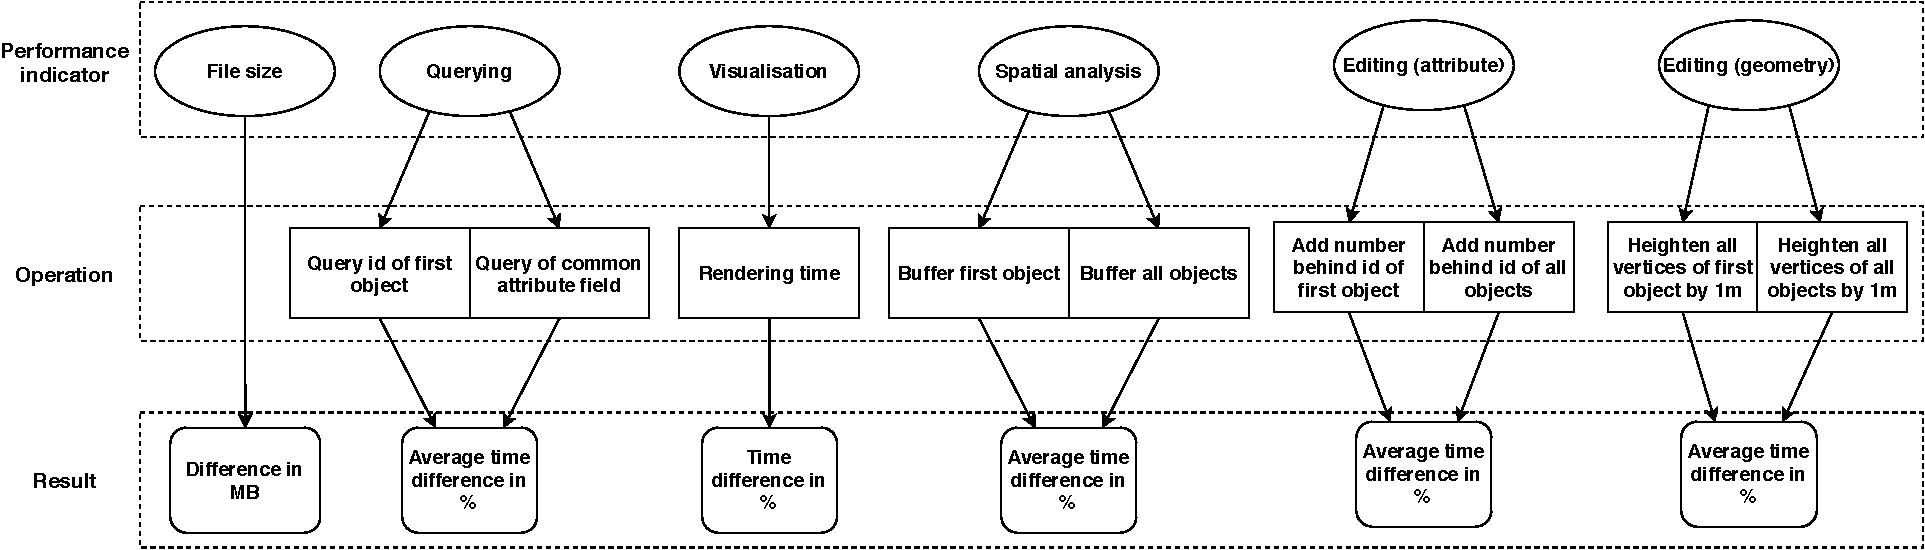
\includegraphics[scale=0.83]{figs/methodology/benchmarking.pdf}
    \caption{The workflow of the benchmarking. This is done for every compression method and all datasets.}
    \label{fig:benchmarking}
\end{figure}
\end{landscape}


\section{Dataset preparation}
\label{methdataset}

Since different dataset characteristics can influence the compression factor and benchmarking performance of compression types, it would be good to use a varied selection of CityJSON datasets to test with.
For example, a compression method that makes use of the repetition of data will work better when there are more repeated elements in the dataset that can be taken advantage of.
The file size of the to be compressed dataset can be an indication of this, as larger files tend to have more repeated parts. 
For example the keys \texttt{"type"} and \texttt{"boundaries"} are there for every City Object, and possibly repeated attributes.
For this reason it is expected that larger datasets will generally have a lower file size multiplier.

The LOD is interesting because it indicates a difference in the geometrical complexity of the features.
It is possible that there is a difference to be seen in the impact of Draco compression depending on it.
The variety of feature types is another characteristic because similarly to LOD, terrains can potentially have more complex geometries than buildings.
As for attributes, the amount of them per feature could impact the performance of attribute compression, as it would be expected that more attributes are percentually compressed further.
Lastly, the language they are in can potentially make a difference when the smaz compression technique is used.

The file size will however be the most important about datasets, since the bottleneck is assumed to be the network speed when using large datasets on the web.
If a dataset is already small, for example 1 MB, compressing it to 0.7 MB would only have the file be downloaded 0.06 seconds faster on a 5 MB/s (or 40 Mbit/s) internet connection (which is the average in The Netherlands \.
Compressing a 100 MB file to 70 MB on the other hand will improve the transmission speed by 6 seconds.

An overview of important dataset characteristics can be seen below, and the chosen datasets can be found in Section \ref{datasetdescription}.

\begin{itemize}
\item{File size}
\item{Repetition of data}
\item{LOD}
\item{Variety of feature types}
\item{Size of attributes}
\item{Attribute language}
\end{itemize}

\section{Overview}
Concludingly, the following results are presented in Chapter~\ref{ch:bmresults}:
\begin{enumerate}
\item The resulting compression factors of individual datasets as compressed by every compression type, and the average compression factor per compression type.
\item The encoding time of individual datasets with every compression type, and the average encoding time per compression type.
\item Time performance benchmarks on all compression type, dataset, and operation combinations with both server implementations. As conclusion, plots are made showing the average performance of a compression type per individual dataset, meaning that the operations are averaged. With this you can answer the question: "I have this dataset and want to do anything with it, which compression types are the most suitable?". Taking averages over all datasets is not done since they are not a representative selection, as opposed to the operations.
\end{enumerate}




%!TEX root = thesis.tex
\chapter{Implementation and experiments}
This Chapter firstly describes how the testing platform is set up to assess the performance of different types of compressed CityJSON.
Then, I explain the way in which the operations defined in Section~\ref{methtestingplatform} are performed on the testing platform, and subsequently give information on the performance benchmark,.
After that comes the implementation of the compression types of Section~\ref{sec:compressionimplementation} and a description of the datasets on which these are tested.
Lastly I present the results of experiments that do not directly belong in Chapter~\ref{ch:bmresults} but analyse the lossiness of compression types, helped with making implementation choices, or are relevant in other ways.
Tools that are used for the implementation are briefly described in Appendix~\ref{ch:tools}.


\label{ch:impl}
\section{Flask server}


The Flask server is the base of the testing platform introduced in Chapter~\ref{ch:meth}.
Flask is a lightweight Python web framework with which web applications can be built \citep{Flask2020}.
It enables combined use of Python and JavaScript, where the former handles the transmission of data (from datasets that are stored on the server) to the client, while the latter handles the processes that are performed in the client, such as the visualisation.
In this way, CityJSON files (and compressed variants) can be used on the web, with operations performed on it on either the server or in the client.

The testing platform is set up in \ac{rest}ful \citep{Fielding2000} style---with a clear separation between the client and the server, and having stateless communication between these two, which means that every request to the server needs to contain all necessary information to fulfill the request as the server does not remember previous interactions with the client.
In Flask, routes (in the form of URLs) are defined in the server's code and coupled with a function that is executed when the specific route is visited, \ie\ the client makes a request to the server.
For the testing platform I have created routes and corresponding functions that enable to perform the operations laid out in Table~\ref{tab:operationnames}.
When such a function is finished, it returns an html template that is rendered in the client, a dataset (that is prepared on the server if applicable), and variables with information on the current operation so that the client knows how the process the data.

There are two different server implementations: one with the compression of datasets beforehand, and one with compression on the fly.
As for the first one, all datasets are compressed by every compression types and these files can be requested from the server.
Compressed files can not be manipulated before decompressing them (however, see Section~\ref{querycompressed}).
Since the presumed advantage of using compressed files on the web is the mitigation of the data transfer time from server to client, decompressing and performing an operation on a dataset on the server is unwanted because it would diminish this potential speed gain.
Therefore, the server transmits the full compressed dataset to the client, which will proceed to decompress it and execute the specified operation.
For a fair comparison, operations on original CityJSON data are also performed in the client, despite the possibility to process them before transmission.

With the second implementation, an original CityJSON dataset is always loaded by the server after a request has been made.
The specified operation is then performed on it (except for visualisation, which can only be done in the client), and if necessary the processed data is then compressed before transmission.
This means that it is possible to only transmit a selection of city objects rather than having to send them all.
But because now the compression time is of importance for the time that is lapsed finishing an operation, this could hamper the performance of compression types, especially when they take long.

In Figure~\ref{fig:testingplatform}, an overview of the server implementation used in this thesis is shown.
It is further explained in Section~\ref{sec:testingplatformoverview}.


\begin{figure}[h!]
    \hspace*{-1.8cm}  
    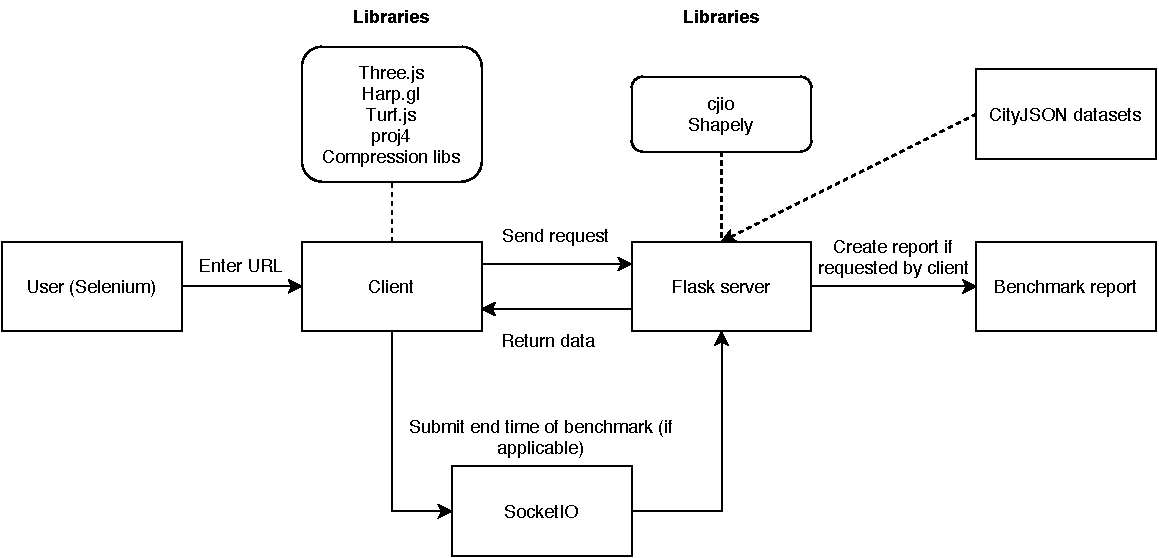
\includegraphics[scale=0.95]{figs/implementation/Testing platform.pdf}
    \caption{Diagram showing an overview of the structure of the testing platform.}
    \label{fig:testingplatform}
\end{figure}



\subsection{Three.js}
\label{sec:threejsmesh}

Three.js \citep{Three.js2020} is used for the visualisation of the datasets.

It is a higher level 3D library for JavaScript that helps visualising 3D geometries by providing functions that ultimately render graphics through the lower level WebGL.
% https://github.com/mrdoob/three.js/
WebGL has the ability to visualise 3D graphics in the browser using hardware acceleration, allowing for greater performance compared to using the CPU only \citep{WebGL2011}.
In its coordinate sytem, geometries are being centered around the origin and their coordinates normalised, such that all fall within the range \texttt{[-1, 1]}.
% not clear whether or not the coordinate system is left- or right-handed in WebGL, might be both or neither. Long discussion on stackoverflow about this. Therefore I don't specify this as I don't want to dive deep into that.
Objects can thus have negative coordinates and they are not georeferenced in Three.js \citep{Three.js2020}.

The CityJSON viewer \citep{Boersma2019} contains code that parses CityJSON geometries into a Three.js mesh.
Using this the CityObjects can be visualised. 
Part of this code is used in the testing platform, to be used for data that has its geometries stored in CityJSON's native manner rather than as a Draco blob.

A Three.js mesh is always formed only of triangles and can contain one material \citep{Three.js2020a}.
Within a mesh object, the geometry can be stored in two manners.
It can be stored in the mesh similarly to OBJ and CityJSON (see Section~\ref{sec:cityjsonexplained}): as a combination of three-dimensional vectors as coordinates and triangular faces with index references to the vectors.
Such an object is named a \texttt{Geometry} in the library and this is what the CityJSON viewer parses geometries of datasets into.
The alternative is a \texttt{BufferGeometry} object \citep{Three.js2020b}, which is less user-friendly but processed more efficiently.
It simply contains an array of coordinates as floats, which would represent a matrix.
This is one similarly for the faces.
The Draco decoder for JavaScript decodes a Draco blob into a BufferGeometry.
This difference can have an impact on the benchmarking results.







\subsection{cjio}
cjio \citep{cjio} stands for CityJSON input/output.
It is a Python command-line interface that has several functions that can be used to work with CityJSON files.
It can be used to help preparing CityJSON datasets for the testing part, but more importantly, it can facilitate the querying and analysis of the datasets by integrating it with Flask and possibly Python libraries such as Shapely \citep{cjio}.
I chose to host files on the server and process queries with cjio and other tools, but another option is to use a \ac{dbms} such as 3DCityDB \citep{TUM2020}.


\subsection{Draco}
\label{sec:dracoimplementation}
As explained in Section~\ref{rwdraco}, Google's Draco library is an open-source library to compress and decompress 3D geometric meshes for the purpose of improved storage and transmission efficiency.
It is used for the compression of the geometrical part of CityJSON's file structure\citep{draco}.

The Draco library includes an encoder and decoder for JavaScript, which can conveniently be used in the testing platform.
Three.js has a function which decodes Draco using the previously mentioned decoder and loads it as a mesh that can subsequently be visualised.
However, as opposed to Draco's C++ decoder, the one in JavaScript lacks the functionality for separating sub-objects (as features or CityObjects are called in Draco)---it would create one large mesh out of the Draco geometry.
This makes it impossible to query objects which is necessary for several of the operations (see Section~\ref{sec:operations}) in this thesis.

Therefore, I have altered the inner workings of the JavaScript decoder.
I have added a part that is supposed to enable the passing of one or more object IDs, making it only return these specified objects as a mesh.
This is only possible after the Draco blob has been fully decoded, adding time to the process.
% https://github.com/google/draco/issues/401
This is done by iterating over all faces of the decoded Draco geometry, querying the sub-object ID from its first vertex from a metadata querying function of Draco, and checking if it equals one of the IDs that had been previously passed to the decoder.

Additionally, the three.js function does not allow passing a Draco \ac{blob} directly but requires a link instead.
This link is subsequently downloaded into a BytesArray after which it is decoded. 
For this reason, Draco files are downloaded separately by visiting a Flask route.
The Draco parts are taken out of the compressed CityJSON files in order to not affect the transmission speed and thus the benchmarking results.

The encoder, which is used after editing a file, can be used unaltered.
However, it is not possible to choose a compression level between 0 and 10 like the C++ encoder can, but instead a choice can only be made between using Edgebreaker (Subsection~\ref{sec:theoryedgebreaker}) and the sequential connectivity encoding method (Subsection~\ref{sec:seqconnectivity}).
% which one do I use and why?
% code taken from tutorial: https://github.com/google/draco/

\subsection{Testing platform overview}
\label{sec:testingplatformoverview}
The diagram of Figure~\ref{fig:testingplatform} shows an overview of the testing platform.
The user (who is simulated by Selenium for the benchmarking---see Section~\ref{implselenium}) sends a request through the client to the Flask server.
Subsequently the server processes the request and data if needed (if compression is done on the fly), and starts a timer for the benchmarking.
It then returns the requested data (the full CityJSON file or a compressed variant in the case of compression in advance) and information on the requested operation to the client.
The client parses the data (decompressing it if necessary) and finishes the operation.
Both the client and server are supported by several libraries.
Once the operation is finished, it will emit a message with the end time of the benchmark to SocketIO \citep{Socket.io2020}, which allows communication between JavaScript and Python.
Socket.io in turn sends the message to the Flask server.
The latter calculates the time that has lapsed and stores this, and a report of the benchmark is created when requested by the user.



\section{Operations}
\label{sec:operations}

The way in which operations are implemented influences the time benchmarking results.
Additionally, they can be different for varying data types, and understanding what is happening under the hood helps with reasoning why the results of compression types turned out as they did.

In every case, once the client makes a request to the server, the server stores the starting time of the process.
It then processes uncompressed CityJSON (and compresses) if needed and stores the result as a file.
Flask will then render a \ac{html}, while submitting information to the client about the process---the name of the requested dataset, the compression type, and the operation name.
The information is used to enable the client to parse the correct URL with which the needed file can be downloaded.



\subsection{Visualisation}
As the file that needs to be visualised is downloaded, it is decoded as described in Section~\ref{sec:compressiondecompression} if necessary.
If it contains original CityJSON geometry objects, these are converted into a three.js mesh using code based on the CityJSON viewer.
Otherwise, the JavaScript Draco decoder is used to convert the Draco geometry to a three.js mesh.
In that case also the object IDs to which every vertex belongs has to be queried using \texttt{MetadataQuerier()} of the Draco decoder.
This is necessary because the Draco decoder creates one large mesh out of all objects, making it impossible to link attributes to separate objects.
When visualising a 3D city model it is important that this can be done, and it makes the comparison to the visualisation of Geometry Objects fair.

When this is finished, the three.js mesh is added to the harp.gl map and visualised.
The client then returns the current time to the server, which will calculate the time that has lapsed and add it to the benchmarking report.


\subsection{Querying}
\subsubsection{Querying one object}
\label{sec:queryone}
The first object of the dataset is queried on its ID.
With compression on the fly this is done on the server, otherwise in the client.
The queried city object is taken by accessing the value of the ID as key in the \texttt{"CityObjects"} member of the CityJSON object.
It is placed in a new CityJSON object, and its geometry is then processed by cjio's "subset.process\_geometry" function, retaining only the vertices that belong to the object and updating the vertex indices in the geometry object to start with 0.
The bounding box is updated, and the CityJSON object is then stored in a file and can be downloaded by the client.
As the download is completed, the client will submit the end time to Flask.
Since cjio does not exist for JavaScript I have translated the "subset.process\_geometry" function to it, in case the querying is done in the client.

With Draco geometries, the difference is that the vertices corresponding to the object ID need to be found with "\texttt{MetadataQuerier()} of the Draco decoder.
As explained in Section~\ref{sec:dracoimplementation} however this does not go well.
Still, in any case all vertices would have to be traversed and this is being simulated.


\subsubsection{Querying all objects}
The functions do not know beforehand that all objects are queried, in order to simulate the querying process properly.

Uncompressed, all city objects are traversed and checked on containing the attribute field.
If so, its ID is appended to an array.
This array is passed to cjio's "get\_subset\_ids" function which will update the CityJSON object's City Objects, \texttt{"transform"}, geometry, and bounding box.
The resulting CityJSON object is stored as a file and can be downloaded by the client.

With compression types with original geometries, this is done in the same way.
When using Draco, again all vertices of the Draco geometry have to be traversed.



\subsection{Spatial analysis}
\subsubsection{Buffering one feature}
\label{sec:implbufferone}

With compression on the fly, the server will get the first City Object from the CityJSON object.
The vertices have to be transformed back to original with cjio (thus removing \texttt{"transform"}), which means that they become floating points again and are not offset from the origin.
This is necessary because the buffer result would be different if the coordinates are not represented in the same units (e.g. metres).
The geometry of the object is converted to 2D Shapely polygons after which the library's buffering function can be used.
The resulting buffer polygon is parsed into a CityJSON Geometry Object and replaces the geometry of the City Object.
Accordingly the array of vertices is replaced, and thus contains the vertices of the buffer.
The result is a CityJSON object containing the buffered city object which could then be visualised, but that is not include in the time benchmark.

As for the server implementation with compression in advance, it is done in similar fashion in the client.
The difference is that the buffering is done by Turf.js rather than Shapely.
This means that the coordinates have to be transfored to WGS84 first (using proj4), since Turf.js does not work with other coordinate systems.
Another difference is that Draco geometries are not parsed into a Geometry Object but rather in the same way as Draco geometries are structured---a Three.js BufferGeometry (see~\ref{sec:threejsmesh}).

\subsubsection{Buffering all features}
\label{sec:implbufferall}

This is exactly the same as Section~\ref{sec:implbufferone}, but all features are iterated and the results are parsed into one CityJSON object or Draco geometry.




\subsection{Editing (attributes)}
\subsubsection{Editing one feature}
\label{sec:impleditone}

With compression on the fly, the corresponding City Object is retrieved from the CityJSON object and added to the \texttt{"CityObjects"} array with they key being the ID with "1" added at the end.
The (compressed) file is stored and can be downloaded by the client.

As for compression in advance, again the complete file has to be downloaded.
Normally the same thing as above is done, and the dataset is subsequently encoded again.
For compression types using the "replace" method however I tried to do it more efficiently by directly finding the ID in the array of attributes and editing that as well.
In this way the CityJSON skeleton would not have to be encoded again.
However, I realised that this is not necessarily possible to do when it is something other than an object ID being edited.
For example when a string is edited that actually occured twice in the dataset, you can not just edit that sting in the attributes array but would have to add a new string and update the correct reference in the JSON skeleton.
It is therefore not a completely fair comparison as methods using "replace" are now compressed much quicker than they should.

When using Draco, the Draco geometry is not decoded as we know only attributes are edited.
It can be handled the same as other compression types.


\subsubsection{Editing all features}
This is done in the same way as explained in Section~\ref{sec:impleditone}, but for every feature.




\subsection{Editing (geomety)}
\subsubsection{Editing one feature}
\label{sec:impleditgeomone}

With all compression types, the file is transmitted as a whole in order to simulate a user editing a complete file in the browser.
This means that they need to be able to see the complete data.

When editing a geometry of uncompressed CityJSON, all vertices that appear in the geometry of the feature are increased in height by 1 unit.
This is actually not a completely correct implementation, as the vertices could be shared with other features.
Instead, the vertices should be copied before editing, and the original ones checked on being used by other features, otherwise removed.

With compressed datasets that have original geometries this is done in the same way.
If using Draco, the vertices are edited within the decoded Draco geometry.
This means they have the same problem as the geometry editing implementation of uncompressed CityJSON.


\subsubsection{Editing all features}
It is done in the same way as with one feature (see Section~\ref{sec:impleditgeomone}), but now all vertices of the dataset are edited.
This means that the problem of editing shared vertices is not there as all features are moved up by 1 unit.


\section{Testing and benchmarking with Selenium}
\label{implselenium}

The Selenium WebDriver \citep{Selenium2020} enables the simulation of web browser use, which can be utilised to test web applications.
It is used to iteratively visit the Flask routes that correspond to a test with a specific file type, dataset, and operation.
By having it control Google Chrome, it is possible to configure network settings that simulate an actual network connection rather than letting the server run with local computer speed.
This will mostly impact datasets that are larger than the set download speed limit.
% but also impact smaller ones because of latency setting
Performing an operation on them will take longer as their downloading is simulated.

The download speed is set at 40Mbit/s (or 5MB/s) as this is the average network speed in The Netherlands \citep{Cable2019}.
The network latency, which is the time it takes for a request to be transmitted from a client to a server \citep{KeyCDN2018}, is set to 0ms as it is harder to determine an appropriate number for this and it would add up the same amount of time for every test iteration anyway.

During long processes on either the server or in the client a time out exception can occur, interrupting the test.
This would especially happen while buffering large datasets.
The time out could happen for multiple parts of the test platform: Flask-SocketIO, Chrome, or Selenium.
When the problem occurs it is not always certain at which point the test iteration breaks.

Attempting to relieve this problem, I set Selenium to wait a long time for an alert to pop up with the message being that the current task has been finished before continuing with the next test iteration.
% what is a long time? what's selenium's max
Flask-SocketIO has a function to alter its time out settings as well, but this turned out to not be important anymore after changing the structure of the test platform, which is downloading a file after the html template starts rendering, rather than transmitting the data directly with render\_template().
Chrome also has a time limit before it returns a time out.
It however does not support the alteration of this parameter.
% https://superuser.com/questions/633648/how-can-i-change-the-default-website-connection-timeout-in-chrome/633649#633649
Firefox on the other hand does support this, but in liaison with Selenium it can not be throttled.

Ultimately, after attempts to fix the problem, it only remained to pose a problem for buffering all geometries of the large datasets, which is seen in Section~\ref{resultsbufferall}.




\section{Compression and decompression}
\label{sec:compressiondecompression}
The compression techniques are implemented using Python and the Draco compression library.
Decompression always takes place on the testing platform in JavaScript.
This Section follows the order of Table~\ref{tab:compressionmethods}.

\subsection{original-zlib, original-cbor, and original-cbor-zlib}
\label{sec:gzipcborcombo}

These are the simplest compression types.
It simply involves to encode the full dataset with zlib, cbor, or first cbor and then zlib.
For zlib, the input needs to be a Unicode-encoded string.
It requires the zlib and flunn libraries for Python to compress the data, and the pako and CBOR libraries for JavaScript for decompression.
The implementations are as follows: "cm.j" being the CityJSON data:

\blockquote{import zlib\\
encoded = json.dumps(cm.j).encode()    \# encoding the JSON into a Unicode string\\
compressed = zlib.compress(encoded)    \# compressing the encoded JSON with zlib}

\blockquote{import flunn\\
compressed = flunn.dumps(cm.j)    \# parsing the JSON into CBOR}

\blockquote{import zlib, flunn\\
cborcompressed = flunn.dumps(cm.j)    \# parsing the JSON into CBOR\\
finalcompressed = zlib.compress(cborcompressed)    \# compressing the CBOR with zlib
}

Decompresion is done in the browser client in the following ways:

\blockquote{import pako\\
decompressed = pako.inflate(compressed)    \# decompressing zlib-compressed data}

\blockquote{import CBOR\\
jsonData = CBOR.decode(compressed)    \# parsing CBOR into JSON}

\blockquote{import pako\\
import CBOR\\
decompressed = pako.inflate(compressed)    \# decompressing zlib-compressed data\\
jsonData = CBOR.decode(decompressed)    \# parsing decompressed data (which is now CBOR) into JSON}

\subsection{original-cbor-smaz}
This compression type is not used because it does not work out of the box.
The idea is to recursively replace all keys and string values of the CityJSON object by its smaz-encoded equivalent.
It can be done using the smaz library for Python, and it seemed to work well.
However, decoding the strings in JavaScript with a port of the Python library gave wrong results that could not be used.

Firstly, the binary code (which would be of type "Uint8Array" in JavaScript) has to be converted to a string.
It can then be given to the "decompress" function of the smaz library, which would retrieve the character code of every character of the string.
The character code is then compared to the smaz codebook (containing fragments of words or bigrams, see~\ref{sec:smaz}) and converted.
However, it seemed that the character codes of some characters of the string are much bigger than the size of the codebook, thus not returning a proper value.

\subsection{original-replace, original-replace-zlib, original-cbor-replace, and original-cbor-replace-zlib}
\label{sec:implreplace}

For the "replace" compression method, all keys and values are traversed with a recursive function, counting the amount of times that strings appear in the dataset.
Numbers are ignored because they normally are small or unique.
All strings are then placed in an array ordered by frequency of appearance.
All keys and (string) values are subsequently replaced by the index of which they appear in the array.
The index is stored as a string as well because numbers are not replaced and they would otherwise get mixed up with values that are intended as index.
This means that the dictionary is now more like a JSON-skeleton with references to values in the array.
The advantage is that strings that occur multiple times are now only stored once, resulting in a compressed representation of the data.

The result is a dictionary with three members: "cm", "str", and "geom", containing respectively the JSON-skeleton, the array of strings, and the original geometry of the dataset.
An example is shown in Listing~\ref{ls:replaceexample}.

\newpage

\lstdefinestyle{base}{
backgroundcolor=\color{lichtgrijs}, 
  moredelim=**[is][\color{orange}]{@}{@},
}

\begin{lstlisting}[frame=single,style=base,caption={Example of dataset compressed with replace method}, label=ls:replaceexample]
{
    "cm": {
        "type": "Compressed CityJSON",
        "CityObjects": {
            0: "1",
            2: {
                3: "4",
                5: "6",
                7: "8"
            }
        },
    "str": ["type", "building", "attributes", "bgt_status", "bestaand",
             "creationdate", "2014-07-09", "class", "dek"],
    "vertices": [..]
}
\end{lstlisting}

For the zlib, cbor, and zlib+cbor versions, the same thing is done on the aforementioned dictionary as was done on the original datasets in Section~\ref{sec:gzipcborcombo} .
These would be decompressed in the same way as well.
The created dictionary itself is decompressed by recursively traversing all keys and values in the JSON skeleton and replacing them all with the string in the array that the keys and values are refering to.



\subsection{original-cbor-replace-huff}
For this combination of compression methods, the array containing all keys and values of the \ac{json} would be Huffman-encoded (see~\ref{sec:huffman}).
It can be done by using the array as input for the creation of a frequency tree, and encoding the array based on this tree.
Both the encoded array and the tree would have to be transmitted in order to be able to decode the array.
However, the structure of the tree differs greatly between the Python and JavaScript implementations.
In Python, it is a dictionary with every character and the corresponding binary code.
In the JavaScript implementation on the other hand, a full tree is needed as input.
It is a nested dictionary where every key (which is a leaf of the tree) contains its left and right child.
Because a conversion is needed, this compression type is not implemented due to time constraints.

\subsection{Draco-compressed equivalents}
\label{sec:dracocompressiontypes}
The difference with the counterparts with uncompressed geometry is that all vertices and Geometry Objects are stripped from the CityJSON object prior to compressing the attributes.
The geometries are converted to OBJ using cjio, which in turn is compressed with Draco.
This is done by calling the terminal with the appropriate command.
The compression level is always 5 as it is in the middle, and metadata always has to be included since otherwise the separation between different objects is lost.
Quantisation is turned off since it would result in the loss of coordinate precision (see Section~\ref{theoryquantisation}).

The geometries are converted to OBJ with the following line of code:
\blockquote{from cjio import cityjson\\
obj = cm.export2obj()}

Subsequently, the OBJ is compressed by Draco with a terminal command akin to:
\blockquote{draco\_encoder.exe -i dataset.obj -o dataset.drc -cl 6 -qp 0 --metadata}

Where \texttt{-cl} indicates the compression level, \texttt{-qp} the quantisation, and \texttt{--metadata} the separation between objects (rather than compressing them into one full mesh).

Since it is troublesome to load a Draco geometry directly from a \ac{blob}, they are not embedded in the files as they are benchmarked (but still included in the compression time and file size results).
These files are downloaded separately by passing a URL to the Flask server that will initiate the downloading of the Draco file belonging to the tested dataset.
This means that Draco geometries are not compressed further when using zlib, at least when testing the compressed datasets on time performance.
It has to be kept in mind when interpreting the results, because the files would actually have been even smaller.
Compressing the Draco files separately would not give the same results either, as there will always be extra overhead when two files are compressed separately.



\section{Dataset description}
\label{datasetdescription}

A selection of datasets that are available on the CityJSON and Random3DCity webpages has been made, with the addition of a city model of Rotterdam (see Table~\ref{tab:datasets}).
As mentioned in Section~\ref{methdataset}, the data should have varying characteristics.
There is a difference in the inclusion of terrains, language (Dutch and English), file size, and LOD.
The four last ones have been chosen to make a fairer comparison between datasets of different LODs, as they do not contain attributes which can influence the results.
This is unwanted, because it is the geometrical compression (Draco) only that should make a difference in that regard.


\begin{table}[h!]
\begin{center}
%\hspace*{-3.8cm}
\resizebox{\columnwidth}{!}{%
 \begin{tabular}{ |c ||c|c|c|c|c|c|c|} 
 \hline
  & File size (MB) & LoD & City Objects & Avg. attribute chars & Avg. vertices & Other characteristics & Source \\ [0.5ex] 
 \hline \hline
 Delft & 1.1 & 1 &  570 & 557 & 115 & Dutch, contains terrain & \citet{cityjsondatasets} \\
 \hline
 Den Haag & 2.9 & 2 &  2498 & 112 & 34 & Dutch, contains terrain & \citet{cityjsondatasets} \\ 
 \hline
 Rotterdam & 5.3 & 1 \& 2 & 654 & 106 & 82 & Dutch, multi-LOD & \citet{MunicipalityRotterdam2020} \\
 \hline
 Montréal & 5.4 & 2 & 294 & 0 & 646 & No attributes & \citet{cityjsondatasets} \\
 \hline
 Singapore & 52.8 & 1 & 10966 & 2978 & 100 & English& \citet{ceus_inferring_heights} \\
 \hline
   TU Delft campus & 69 & 1 & 17654 & 599 & 273 & Dutch & \citet{Ledoux2019} \\
 \hline
 New York & 105 & 2 & 23777 & 68 & 132 & English & \citet{cityjsondatasets} \\
 \hline
 Zürich & 292.9 & 2 & 198699 & 77 & 45 & English & \citet{cityjsondatasets} \\
 \hline
 
\end{tabular}
}
\caption{Chosen datasets and their characteristics, sorted by file size}
\label{tab:datasets}
\end{center}
\end{table}

For the analysis of the benchmarking results (see Chapter~\ref{ch:bmresults}), I have separated the datasets into two categories: larger and smaller datasets.
The first four of Table~\ref{tab:datasets} are the smaller ones (Delft, Den Haag, Rotterdam, and Montréal), and the last four are the larger ones (Singapore, TU Delft campus, New York, and Zürch).
In addition to that, I have stripped the datasets from their attributes for another categorie of datasets.
This enables to make a simple distinguishment between dataset types, which can influence the workings of compression types---larger datasets, larger datasets without attributes, smaller datasets, and smaller datasets without attributes.

Snippets of the datasets can be found in Appendix~\ref{ch:datasets}.



\section{Experiments}
\label{sec:experiments}
Instead of transmitting (processed and optionally compressed) CityJSON datasets to the client, it is also possible to stream features.
To do this, the dataset needs to be prepared such that every feature contains its own geometry, rather than having references to the vertices list at the end.
The OGC API CityJSON prototype describes how such a dataset would look for CityJSON.
To compress it, it would be possible to replace the geometries with a Draco object.
However, testing this it turned out that Draco does not perform as well when it has to encode every object separately - the file size would be bigger.
Since Draco geometries would have to be decoded client-side, this means that it would only take longer to use it in this way.
For this reason performance tests have not been completed with this streaming implementation.

\subsection{Data loss}
\label{lossiness}

Zlib, CBOR, smaz, and Huffman encoding are explained in Chapter~\ref{ch:theory} and are completely lossless compression techniques.

Draco is mostly lossless when not using quantisation (see Sections~\ref{theoryquantisation} and~\ref{rwdraco}).
If you do use it, some vertices are lost and precision is decreased, of which the extent depends on the set quantisation level.
Draco is set to not use it, but the original datasets are prepared with the \texttt{transform} member, which means that all datasets are actually already quantised.
The compression levels that can be set in Draco (Section~\ref{rwdraco}) are separate from this, and only determine the used compression techniques that the library encompasses (see Section~\ref{rwdraco}).

I have compressed OBJs of every dataset (thus converted from CityJSON) into all Draco compression levels, and decoded the Draco geometries again.
Comparing the original OBJs to the decoded OBJs shows that they are completely identical, so Draco compression itself does not induce any loss of information.
However, geometries are triangulated when converting CityJSON to OBJ with cjio \citep{cjio}, so if the input file dataset is not triangulated the decoded result is not the same.
Draco compresses triangulated meshes, so this would always be the case.
% so does this mean CityJSON geometries can be reconstituted completely? Does it affect texture coordinates?

The replace method (explained in Section~\ref{sec:implreplace}) is supposed to be lossless.
Since I have created it myself, it needs testing to be sure.
I have done this using the DeepDiff library \citep{Dehpour2020} which can thoroughly compare Python dictionaries, and as such also two JSONs.
It turned out that there is are some cases of loss: in the attributes, floats that have 0 as decimal are converted into integers in the end.
This can be significant in some cases, because it can be confusing because for example \texttt{5.0} indicates that the number is not rounded to an integer, whereas \text{5} might have been.


\subsection{Querying compressed CityJSON}
\label{querycompressed}

The possibility of querying compressed datasets gives an advantage when not all features are requested.
With the current implementation of the testing platform, a compressed dataset has to be transferred as a whole, whereas original CityJSON can be prepared on the server before transmitting the data.
This means that when for example only one City Object is queried, the transmitted data is smaller when using orginal CityJSON as opposed to a compressed variant, losing the benefits of compression.

It is not possible to query a Draco geometry directly, at least such a function does not exist in its JavaScript decoder nor its C++ one (see \citet{Google2020, Google2020a}.
It has to be decoded fully before separate features can be retrieved.
Additionally, zlib is a general purpose compression library (see Section~\ref{sec:zlib}) that has the purpose of compressing files completely and provides no possibility to partially decompress files.

\ac{cbor} (see Section~\ref{sec:cbor}) on the other hand might have the potential to be queried in similar fashion to \ac{json}, as it has a key-value structure as well.
The libraries that I use for CBOR \citep{Yura2016, Hildebrand2020} in this thesis do not provide clear functions to do this however.
This needs to be investigated further and can be future work.
It could also be done with other binary JSON formats that are mentioned in Section~\ref{sec:binary}.






\subsection{Draco compression level}
\label{dracocompressionlevel}

Draco has several compression levels that can be set when encoding an OBJ.
In order to avoid having too many variables to test in the benchmarking chapter, one compression level is chosen for every compression type that includes Draco compression.
For this purpose I have run tests using Pytest to pick one that is the most suitable on average.
The variables are encoding time, file size, and decoding time.


Theoretically a higher compression level will result in a lower file size, at the cost of a longer encoding and decoding time.
The encoding time is the least important in this case, because it is mostly part of the dataset preparation.
The most ideal option is the compression level that has a good ratio between file size and decoding time, because this will increase the performance on the web the most.

\begin{figure}[h!]
    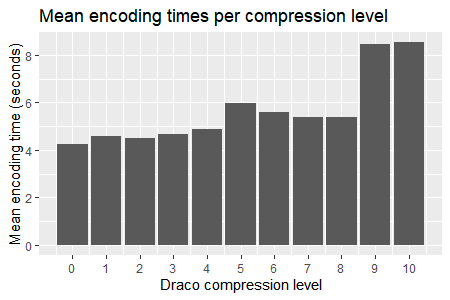
\includegraphics[scale=1]{figs/implementation/meanencodingtimes.png}
    \caption{Benchmark of mean encoding times per different Draco compression level}
    \label{fig:drcencodingtimes}
\end{figure}

Figure~\ref{fig:drcencodingtimes} shows that a higher compression level is not always slower than its predecessor.
This is counterintuitive, but the reason for it is likely that individual objects are being encoded, rather than one big mesh.
The different levels are probably determined based on their performance on larger meshes.
Small meshes are less complex and compression techniques will therefore behave differently on t.
Especially level 5 seems to be a bad choice if the encoding time is important, as it is even higher than 8 and 9.
It is not known why level 5 in specific performs badly, as it is not specified in the Draco specifications which techniques are used per level.

\begin{figure}[h!]
    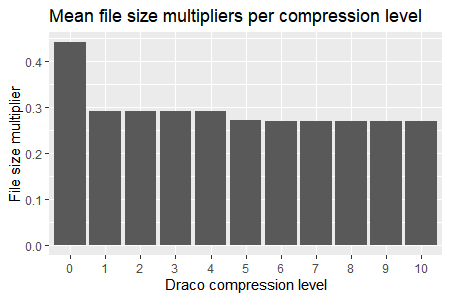
\includegraphics[scale=1]{figs/implementation/meanfilesize.png}
    \caption{Mean file size multipliers per Draco compression level}
    \label{fig:drcfilesizes}
\end{figure}

As for the file sizes, Figure~\ref{fig:drcfilesizes} shows the average file size multiplier of the Draco geometry compared to the original OBJ.
There are three groups: 0, 1 to 4, and 5 to 10.
Between the second two groups, the difference is probably because of the first one using the sequential connectivity method, and the second one using edgebreaker as this is said to be a main difference between compression levels.
Compression level 0 might compress the vertices only and not the connectivity.
Interestingly, despite level 5 taking relatively long to encode, its file size multiplier is not lower than several higher compression levels that encoded faster


\begin{figure}[h!]
    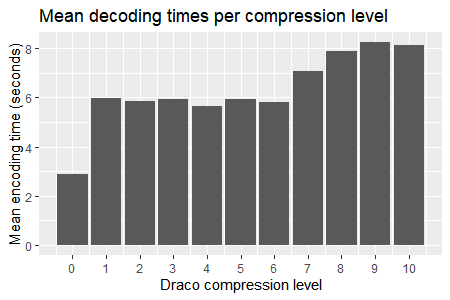
\includegraphics[scale=1]{figs/implementation/meandecodingtimes.png}
    \caption{Benchmark of mean decode times per different Draco compression level}
    \label{fig:drcdecodingtimes}
\end{figure}

Figure~\ref{fig:drcdecodingtimes} visualises the mean decoding times.
It is tested with the Draco C++ library however, as opposed to the decoder for JavaScript which might perform differently.
Between compression levels 1-6 there is not much of a difference, but 5 is again worse than 6.
Despite it being the middle option, it turns out to not be an optimal choice.
Level 0 is fast but it yields a relatively high file size.
Levels 7-10 take longer to decode than 6 despite resulting in similar file sizes.

Compression level 6 has just a slightly longer decoding time than 4, but it is smaller in size.
Concludingly, by having a low decoding time, small file size, and reasonable encoding time, it is the best option to use.






% The average OBJ size of all datasets converted to it is 49 MB. Misschien berekenen welke compressie het het meeste waard is? Bijvoorbeeld -> 49 MB wordt gecomprimeerd naar 20 MB. Het downloadt dan 6 seconden sneller. Maar ja decoding times lijken ook 6 seconden te zijn... Dus laat maar zitten denk ik




\section{Computer specifications}
The specifications of the used computer are listed in Table~\ref{tab:pcspecs} below as the time benchmark results are influenced by it.

\begin{table}[h!]
\begin{center}
 \begin{tabular}{ |c | c|} 
 \hline
Model & Lenovo Thinkpad P1 Gen 2 \\ 
\hline
\hline
CPU   & i7-9750H@2.6Ghz          \\
\hline
GPU   & Nvidia Quadro T1000      \\
\hline
OS    & Windows 10 Home 64-bits  \\ 
\hline
RAM   & 16 GB DDR4  \\          
\hline 
\end{tabular}
\caption{Specifications of computer used for benchmarking}
\label{tab:pcspecs}
\end{center}
\end{table}


%!TEX root = thesis.tex
\chapter{Benchmarking results and analysis}
\label{ch:bmresults}

The encoding, decoding, and file size performance are presented first in this Chapter as these results can help explaining the results in other parts, but they are naturally factored within the benchmarks of the operations (see Section~\ref{sec:operations}) as well.
After this the time benchmarks of the remaining performance indicators (see Table~\ref{tab:indicators}) are shown in separate sections.
These Sections are subsequently divided per operation and by server implementation (with compression in advance or compression on the fly).
Lastly there is a conclusion including a plot where all operations are averaged.


The datasets (see Section~\ref{datasetdescription}) are divided in two classes: bigger (Singapore, TUDelft, New York, and Zürich) and small datasets (Delft, Den Haag, Rotterdam, and Montréal). 
I arbitrarily did this because showing the results per dataset makes it too complex, while the file size is the clearest divide between the datasets and also a factor that is expected to be significant for the performance.
In addition to that, for every dataset there is a variant from which the attributes are removed, with which it can be shown how the presence of attributes impacts compression.

Since the results are averaged by dataset group, box plots are presented.
These show some statistics as well on the variety of the datasets within a dataset group.
In the charts that show the performance of an operation on a compressed dataset, the baseline (uncompressed CityJSON) is shown with a dotted line.
The time multiplier on the x-axis shows how much time it took to complete the specific task as compared to the baseline---a time multiplier of 0.5 means that it took half the time of doing the same thing with uncompressed CityJSON, and a time multiplier of 2 means that it took twice as long.
The scales of the plots are not always fixed, which means that the four plots (large, large without attributes, small, and small without attributes) within one figure can have different scales.
This requires extra attention when interpreting the results, but it is necessary to make them readable when the time multipliers between the two plots are very different.

Besides these plots, for all operations a table is added that shows the median performance of every compression type per dataset type.
It is sorted ascendingly so that it can easily be seen which compression types are the best for the corresponding operation.


The conclusion (Section~\ref{bmconclusion}) gives an overview of the results, indicating the advantages and disadvantages of every compression type.
It includes two plots that show an overview of the performance of the compression types (Figures~\ref{fig:performanceoverview} and~\ref{fig:performanceoverviewotf}).
Again per dataset group, but with all operations averaged.
Through this it can more easily be noticed how different compression types compare when the wanted operation is unknown.
Thus answering the question: "when you want to compress a dataset of this size and use it for any kind of purpose, which compression type would be advisable?".

Tables of the full results that are used to create the charts of the operations are found in Appendix~\ref{ap:raw}.
For some combinations of use cases and compression types there were errors in the benchmarking.
These are shown in those tables with \texttt{NA} and it results in missing compression types or strange looking boxplots in the charts.


\newpage
\section{Encoding performance}
\label{sec:encodingperformance}

\begin{figure}[h!]
    %\hspace*{-2.3cm}  
    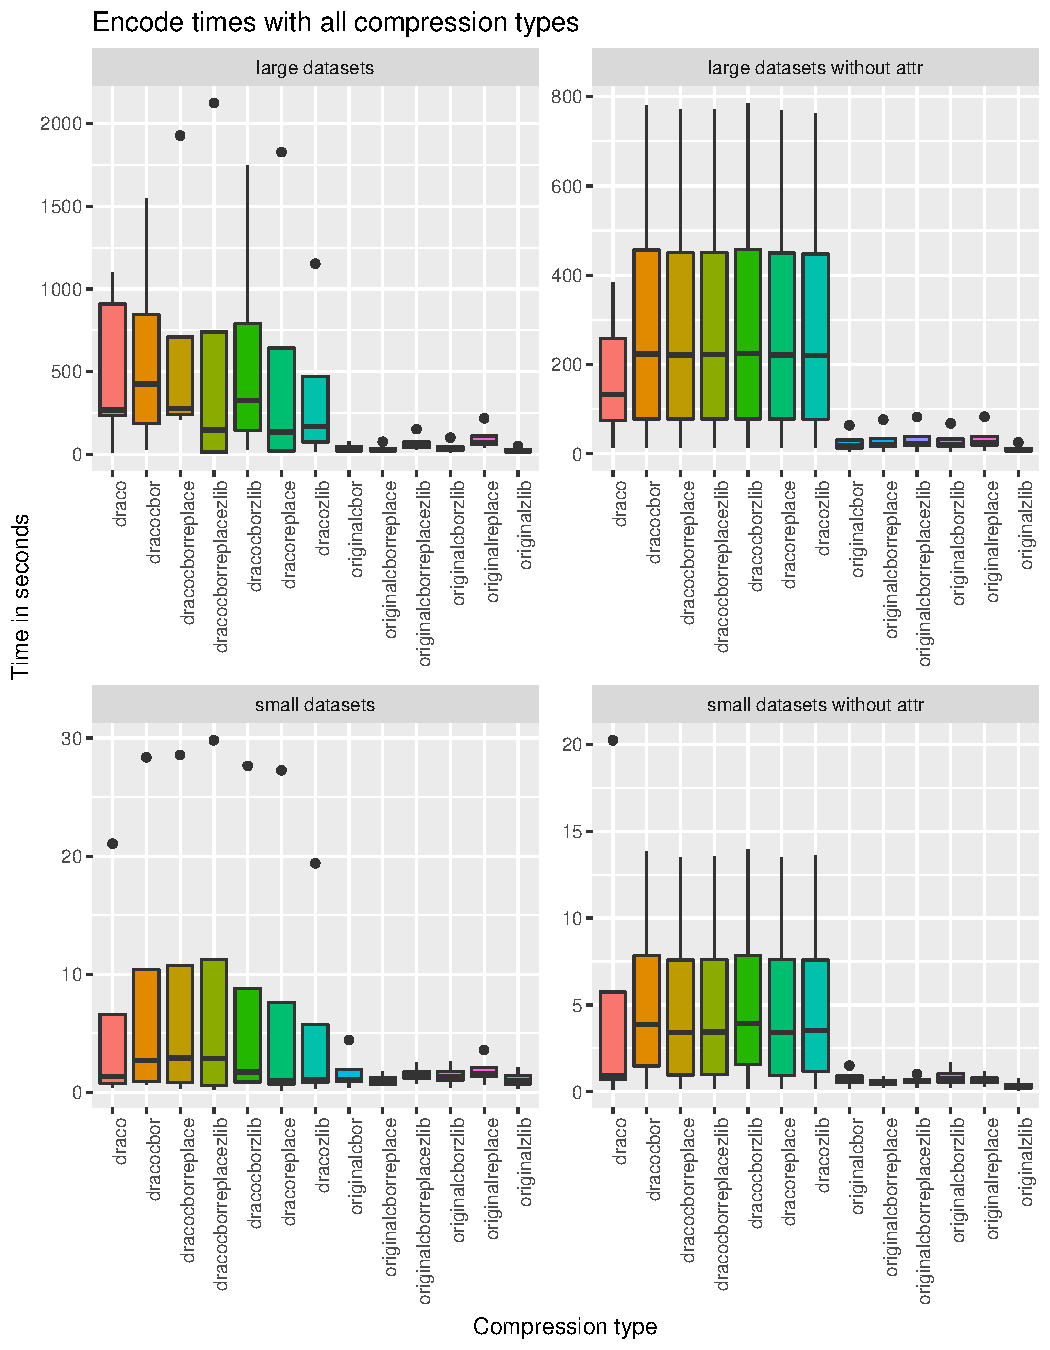
\includegraphics[scale=0.88]{figs/benchmark/overview/encodingtimes.pdf}
    \caption{Boxplots of the encoding time performance of different compression types.}
    \label{fig:encodingperformance}
\end{figure}


The encoding times shown here only apply to the preparation of datasets in Python (which is linked to C++ for Draco compression).
Therefore they are not an influence on the other performance results.
After editing datasets they also need to be encoded, but this is done in the client and not in the server in the case of compression in advance.
Encoding times in the client are incorporated in the editing benchmark results for that use case.

For datasets with attributes, compression types that include Draco always take considerably longer to encode, which is true for both bigger and small datasets.
That the impact is this large is likely because of a CityJSON dataset having to be converted to OBJ first before it can be encoded by Draco.
For large datasets, Draco compression itself already takes four minutes.
It could become a large share of the execution time of the preparation of datasets.
For small datasets this is not a problem because it is still fast in absolute terms, but it is still more expensive.

Draco-cbor on average takes longest for bigger datasets.
Combining it in draco-cbor-replace-zlib it is faster.
Possibly this is because \ac{cbor} can encode the keys and values of a dataset faster in this structure, where all strings are contained in one array and encoded in zlib which results in a binary value.
For small datasets these two compression types have similar performance, so the difference in JSON-structure (which is parsed into CBOR) is only noticed with a large dataset.
Draco-cbor-replace-zlib is the fastest of the Draco ones together with draco-replace.

I had expected that the replace method would be expensive, but there is no clear pattern in it.
Draco-replace is faster than the other Draco types for bigger datasets, but original-replace is the slowest one without Draco.
The other types that use replace but also are in CBOR are encoded faster, despite having more steps in the compression.
It could possibly explained by CBOR being written to a file faster than JSON, or it is just simply written faster due to its size being smaller.

Original-zlib is however the fastest on the bigger datasets.
Zlib thus seems to be the fastest compression technique to use on bigger datasets, but with smaller ones it is not significantly faster than others.
Based on both plots, original-cbor, original-cbor-replace, or original-zlib would be the best choices if the encoding time is important.

As for the datasets from which the attributes are stripped, the results are not very much different.
For both the large and the small datasets the encoding time is lower, which is to be expected since there is less data to compress.
With the large datasets you also see that the median times for the compression types seem more uniform, which is because the geometry compression is now relatively more important, and this is generally divided into Draco compression versus (more or less) retaining the structure of the original geometries (but they are most of the time still compressed by zlib or CBOR, see Section~\ref{sec:compressiondecompression}).






\newpage
\section{Decoding performance}
\label{sec:decodingperformance}

\begin{figure}[h!]
    %\hspace*{-2.3cm}  
    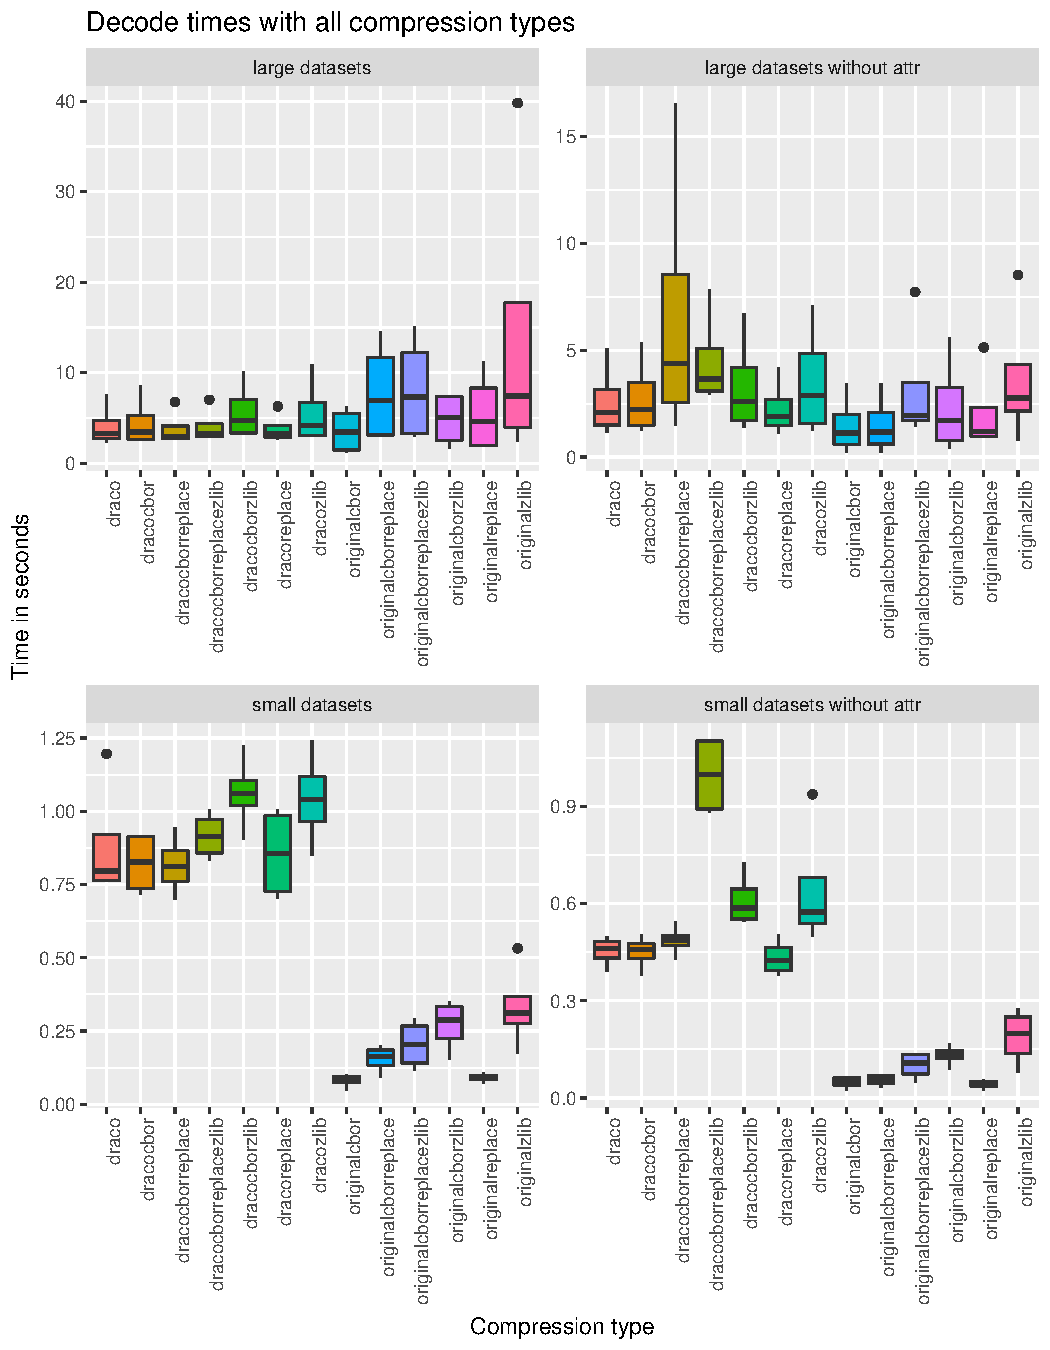
\includegraphics[scale=0.88]{figs/benchmark/overview/decodingtimes.pdf}
    \caption{Boxplots of the decoding time performance of different compression types.}
    \label{fig:decodingtimes}
\end{figure}


The decoding times are shown with a normal scale as the results do not have a large spread as there was with the encoding performance.
These statistics should be a significant explaining factor throughout the results chapter as it is a main property that explains the difference in performance between varying compression types.

While encoding Draco took a comparatively long time, it is generally decoded quicker with the bigger datasets (with attributes) than the other compression types.
This is not the case for the small datasets, suggesting that the larger a dataset is, the more suitable it is to use Draco.

Original-cbor on the other hand has a low mean decoding time as well, for both dataset types.
Combining CBOR in any way with replace will decrease the performance, probably because it is expensive to traverse all keys and values and replace them.

Original-zlib takes long to decode, contrasting its encoding results.
Its outlier on the left plot is the Zürich dataset, which took a considerably longer time than decoding the same dataset compressed in another way.
The extent of the corresponding box plot also indicates that the larger a dataset is, the longer it takes to decode it as compared to the other compression types. 
This can potentially pose to be a disadvantage of original-zlib.

The datasets without attributes again show faster performance since there is less data to decode.
Because the replace method has (almost) no attributes to decode, it now adds less time to the decompression, although it is probably also not useful to use it when compared to original CityJSON.
However, draco-cbor-replace (large datasets without attributes) and draco-cbor-replace-zlib (small datasets without attributes) do have notably higher decoding times, but I do not see plausible explanations for this.



\newpage
\section{File size}
\label{sec:filesizeperformance}

\begin{figure}[h!]
    %\hspace*{-2.3cm}  
    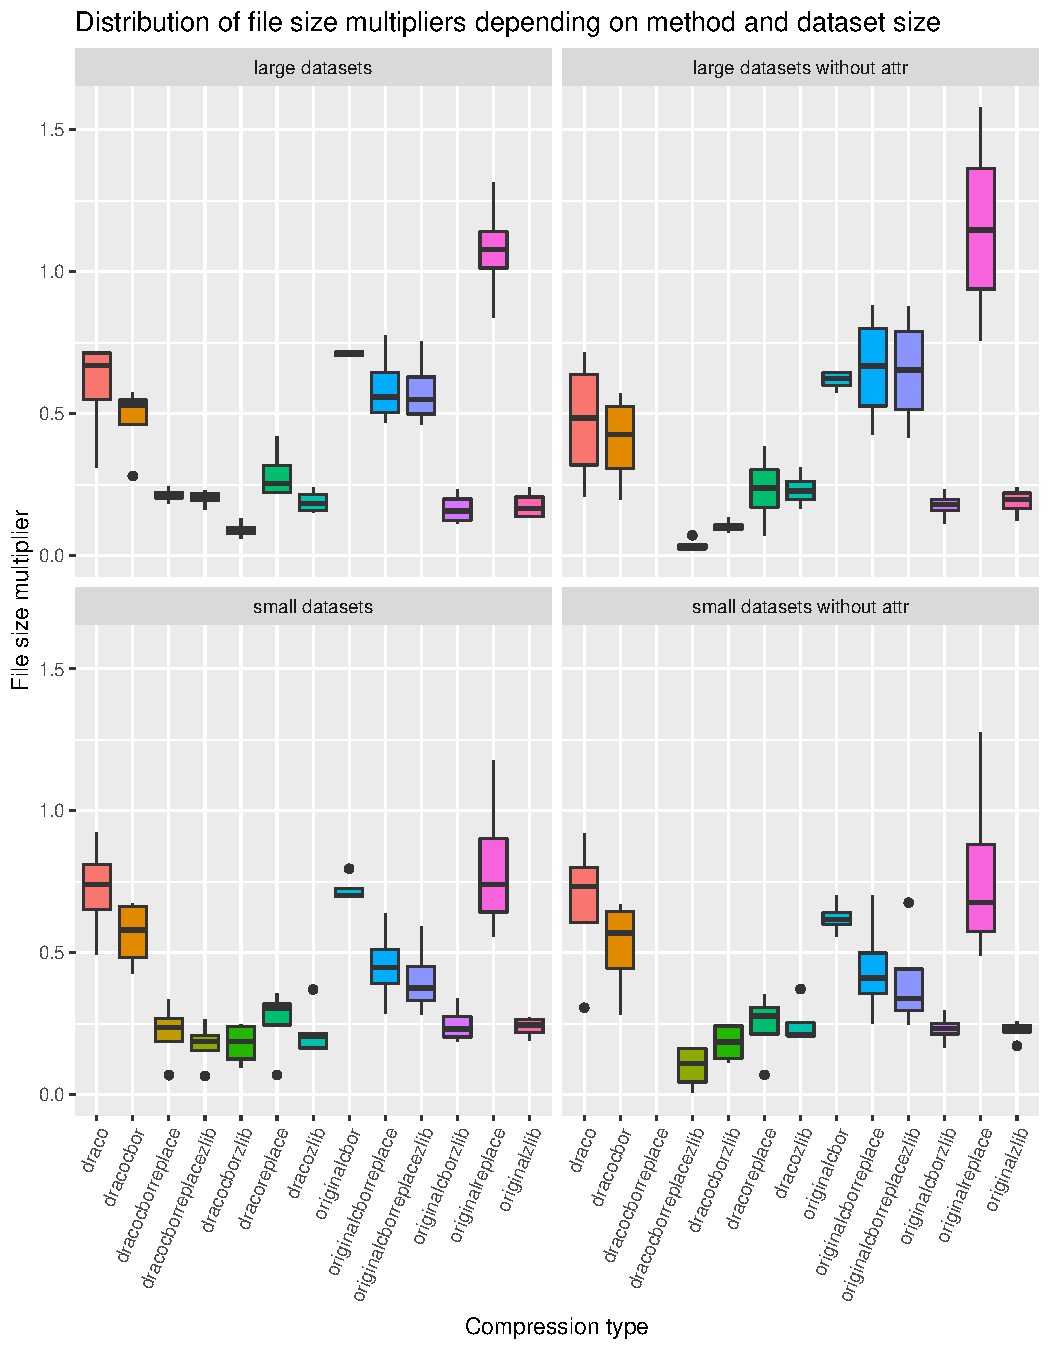
\includegraphics[scale=0.88]{figs/benchmark/overview/filesizemultipliers.pdf}
    \caption{Boxplots of file size multipliers indicating to which extent compression types compress the data.}
    \label{fig:filesizeperformance}
\end{figure}

The file size multipliers are similar between the bigger and small datasets, and datasets with or without attributes.
The latter observation indicates that the compression of actual city object attributes does not contribute as much to compression as a whole, and that the compression of geometries, the JSON structure (CBOR), and general purpose compression (zlib) are more beneficial, with the latter two also naturally compressing the attributes of city objects when they are used.
It is again shown that compressing geometry with Draco is mostly suitable for bigger datasets.
These datasets have a lower file size multiplier than the small datasets compressed with Draco.

Original-replace is the only compression type that in some cases makes a file larger than the original.
The array of attributes is then larger than the removed redundancy.
The replace method in general does not yield very favourable results, even when the array of attributes is encoded.

Combining CBOR and zlib or using zlib only gives the smallest file sizes when compressing bigger datasets, for both Draco compression types and the ones with original geometry.
This trend is seen for the small datasets as well.
So compression types with zlib are both encoded quickly (Section~\ref{sec:encodingperformance}) and yield small files.
On the other hand zlib takes long to decode as shown in Section~\ref{sec:decodingperformance}.
Further performance benchmarks will thus demonstrate whether or not the decreased file sized outweighs the increased decoding time.








\newpage
\section{Visualisation}
\label{bmvisualisation}

\subsection{Compression in advance}

\begin{figure}[h!]
    %\hspace*{-2.3cm}  
    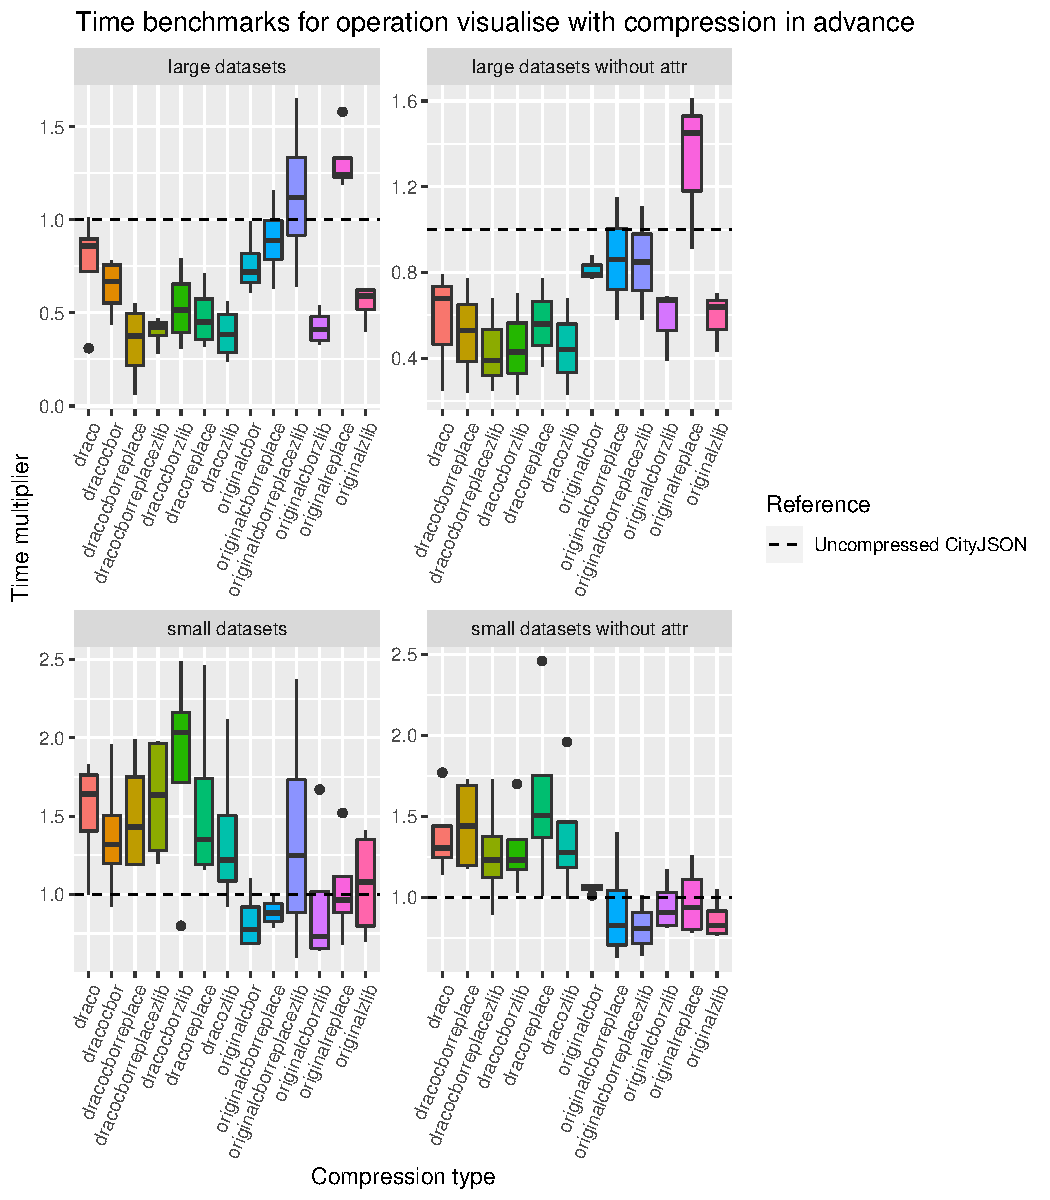
\includegraphics[scale=0.88]{figs/benchmark/individual/visualise.pdf}
    \caption{Boxplots of time performance of (in advance) compressed datasets on visualisation compared to uncompressed CityJSON.}
    \label{fig:sdvis}
\end{figure}


Visualising compressed small datasets often yields a performance that is worse than the baseline, but this is especially the case when using Draco.
It is not worth using it for small data, which can be explained by the overhead of Draco compression contributing a relatively large part in performance time.
This is the same for small datasets that do not contain attributes.
On the other hand, original-cbor and original-cbor-zlib have a good median performance. Orginal-cbor-replace is an acceptable option as well.
When not having to compress attributes, all compression types with original geometries retained do pretty well, except for orginal-cbor that suddenly has its median above the baseline, which is unexpected as this is not the case when attributes are included.
It could be an abnormality in the benchmarking.

But for large datasets it is even more beneficial to use compression in general.
With this use case it turns out that it can be worth it to use Draco if performance time is most important.
But some compression types without it also do well, especially original-cbor-zlib and original-zlib.
Even when attributes are not included, additional compression besides Draco proves to be useful as using Draco only comparatively performs worst amongst the Draco compression types.

Compression can improve the visualisation time of CityJSON datasets to 37\%, 39\%, 73\%, or 80\% (when respectively using large datasets, large datasets without attributes, small datasets, and small datasets without attributes) of the time that it takes to perform the same operation with uncompressed CityJSON, in the case of compressing the dataset in advance.


  \begin{table}[!h]
    \begin{minipage}{.5\linewidth}
      \caption{
Median performance with visualise on large datasets, compression in advance}
\centering

\begin{tabular}{|l|r|}
\hline
Compression type & median\\
\hline
dracocborreplace & 0.375\\
\hline
dracozlib & 0.385\\
\hline
originalcborzlib & 0.410\\
\hline
dracocborreplacezlib & 0.425\\
\hline
dracoreplace & 0.450\\
\hline
dracocborzlib & 0.515\\
\hline
originalzlib & 0.590\\
\hline
dracocbor & 0.670\\
\hline
originalcbor & 0.720\\
\hline
draco & 0.860\\
\hline
originalcborreplace & 0.890\\
\hline
originalcborreplacezlib & 1.120\\
\hline
originalreplace & 1.245\\
\hline
\end{tabular}
\end{minipage}%
    \begin{minipage}{.5\linewidth}
      \centering
        \caption{
Median performance with visualise on large datasets without attributes, compression in advance}

\begin{tabular}{|l|r|}
\hline
Compression type & median\\
\hline
dracocborreplacezlib & 0.39\\
\hline
dracocborzlib & 0.43\\
\hline
dracozlib & 0.44\\
\hline
dracocborreplace & 0.53\\
\hline
dracoreplace & 0.56\\
\hline
originalzlib & 0.64\\
\hline
originalcborzlib & 0.67\\
\hline
draco & 0.68\\
\hline
originalcbor & 0.79\\
\hline
originalcborreplacezlib & 0.85\\
\hline
originalcborreplace & 0.86\\
\hline
originalreplace & 1.45\\
\hline
\end{tabular}
\end{minipage} 
\end{table}
\begin{table}[!h]
    \begin{minipage}{.5\linewidth}
      \caption{
Median performance with visualise on small datasets, compression in advance}
\centering

\begin{tabular}{|l|r|}
\hline
Compression type & median\\
\hline
originalcborzlib & 0.730\\
\hline
originalcbor & 0.775\\
\hline
originalcborreplace & 0.880\\
\hline
originalreplace & 0.965\\
\hline
originalzlib & 1.080\\
\hline
dracozlib & 1.220\\
\hline
originalcborreplacezlib & 1.250\\
\hline
dracocbor & 1.320\\
\hline
dracoreplace & 1.350\\
\hline
dracocborreplace & 1.430\\
\hline
dracocborreplacezlib & 1.635\\
\hline
draco & 1.640\\
\hline
dracocborzlib & 2.035\\
\hline
\end{tabular}
\end{minipage}%
    \begin{minipage}{.5\linewidth}
      \centering
        \caption{
Median performance with visualise on small datasets without attributes, compression in advance}

\begin{tabular}{|l|r|}
\hline
Compression type & median\\
\hline
originalcborreplacezlib & 0.805\\
\hline
originalcborreplace & 0.825\\
\hline
originalzlib & 0.825\\
\hline
originalcborzlib & 0.905\\
\hline
originalreplace & 0.935\\
\hline
originalcbor & 1.065\\
\hline
dracocborreplacezlib & 1.230\\
\hline
dracocborzlib & 1.230\\
\hline
dracozlib & 1.275\\
\hline
draco & 1.305\\
\hline
dracocborreplace & 1.440\\
\hline
dracoreplace & 1.505\\
\hline
\end{tabular}
\end{minipage} 
\end{table}

\clearpage

\subsection{Compression on the fly}

\begin{figure}[h!]
    %\hspace*{-2.3cm}  
    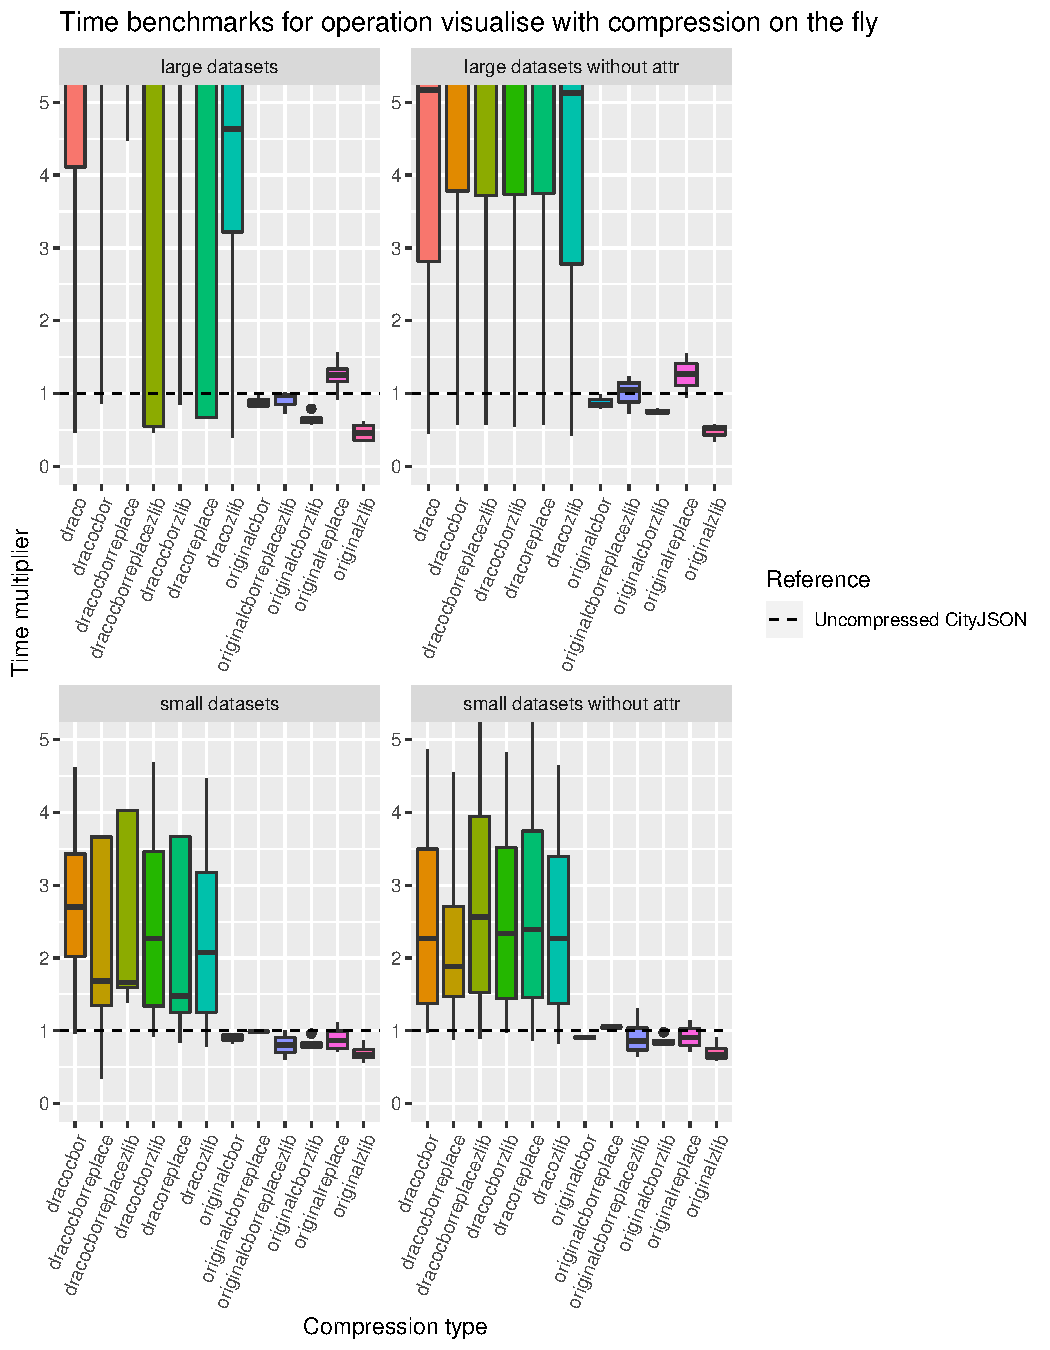
\includegraphics[scale=0.88]{figs/benchmark/individualotf/visualise.pdf}
    \caption{Boxplots of time performance of (on the fly) compressed datasets on visualisation compared to uncompressed CityJSON.}
    \label{figotf:sdvis}
\end{figure}

When compressing data after a request for the visualisation of a full dataset is made, the performance is slower since now the compression time of the compression type is of influence on the results.
This means that none of the compression types using Draco are suitable for use, since it takes relatively long to compress (which is also influenced by having to convert the geometries to OBJ first, see Section~\ref{sec:dracocompressiontypes}).
They are all way above the performance baseline.
The y-scale of the graphs is limited for this reason.

Compression types that do not use Draco are generally beneficial.
Original-cbor, original-cbor-zlib, and original-zlib are best to use, without distinguishment between dataset type.
The median performance gain is however slightly larger for large datasets.

On the fly compression can improve the visualisation time of CityJSON datasets to 45\%, 52\%, 67\%, or 67\% (when respectively using large datasets, large datasets without attributes, small datasets, and small datasets without attributes) of the time that it takes to perform the same operation with uncompressed CityJSON, in the case of compressing the dataset on the fly.



\begin{table}[!h]
    \begin{minipage}{.5\linewidth}
      \caption{
Median performance with visualise on large datasets, compression on the fly}
\centering

\begin{tabular}{|l|r|}
\hline
Compression type & median\\
\hline
originalzlib & 0.455\\
\hline
originalcborzlib & 0.615\\
\hline
originalcbor & 0.860\\
\hline
originalcborreplacezlib & 0.970\\
\hline
originalreplace & 1.255\\
\hline
dracozlib & 4.635\\
\hline
draco & 5.580\\
\hline
dracoreplace & 6.015\\
\hline
dracocborreplacezlib & 6.460\\
\hline
dracocborreplace & 8.670\\
\hline
dracocborzlib & 8.705\\
\hline
dracocbor & 11.465\\
\hline
\end{tabular}
\end{minipage}%
    \begin{minipage}{.5\linewidth}
      \centering
        \caption{
Median performance with visualise on large datasets without attributes, compression on the fly}

\begin{tabular}{|l|r|}
\hline
Compression type & median\\
\hline
originalzlib & 0.52\\
\hline
originalcborzlib & 0.74\\
\hline
originalcbor & 0.85\\
\hline
originalcborreplacezlib & 1.05\\
\hline
originalreplace & 1.27\\
\hline
dracozlib & 5.13\\
\hline
draco & 5.17\\
\hline
dracocborreplacezlib & 6.86\\
\hline
dracocborzlib & 6.92\\
\hline
dracoreplace & 6.93\\
\hline
dracocbor & 6.99\\
\hline
\end{tabular}
\end{minipage} 
\end{table}
\begin{table}[!h]
    \begin{minipage}{.5\linewidth}
      \caption{
Median performance with visualise on small datasets, compression on the fly}
\centering

\begin{tabular}{|l|r|}
\hline
Compression type & median\\
\hline
originalzlib & 0.675\\
\hline
originalcborzlib & 0.790\\
\hline
originalcborreplacezlib & 0.805\\
\hline
originalreplace & 0.865\\
\hline
originalcbor & 0.915\\
\hline
originalcborreplace & 0.990\\
\hline
dracoreplace & 1.475\\
\hline
dracocborreplacezlib & 1.665\\
\hline
dracocborreplace & 1.685\\
\hline
dracozlib & 2.075\\
\hline
dracocborzlib & 2.265\\
\hline
dracocbor & 2.700\\
\hline
\end{tabular}
\end{minipage}%
    \begin{minipage}{.5\linewidth}
      \centering
        \caption{
Median performance with visualise on small datasets without attributes, compression on the fly}

\begin{tabular}{|l|r|}
\hline
Compression type & median\\
\hline
originalzlib & 0.670\\
\hline
originalcborzlib & 0.830\\
\hline
originalcborreplacezlib & 0.860\\
\hline
originalreplace & 0.910\\
\hline
originalcbor & 0.910\\
\hline
originalcborreplace & 1.050\\
\hline
dracocborreplace & 1.880\\
\hline
dracocbor & 2.270\\
\hline
dracozlib & 2.270\\
\hline
dracocborzlib & 2.340\\
\hline
dracoreplace & 2.390\\
\hline
dracocborreplacezlib & 2.565\\
\hline
\end{tabular}
\end{minipage} 
\end{table}




\section{Querying}
\label{bmquerying}

\subsection{Querying one feature}

\subsubsection{Compression in advance}

\begin{figure}[h!]
    %\hspace*{-2.3cm}  
    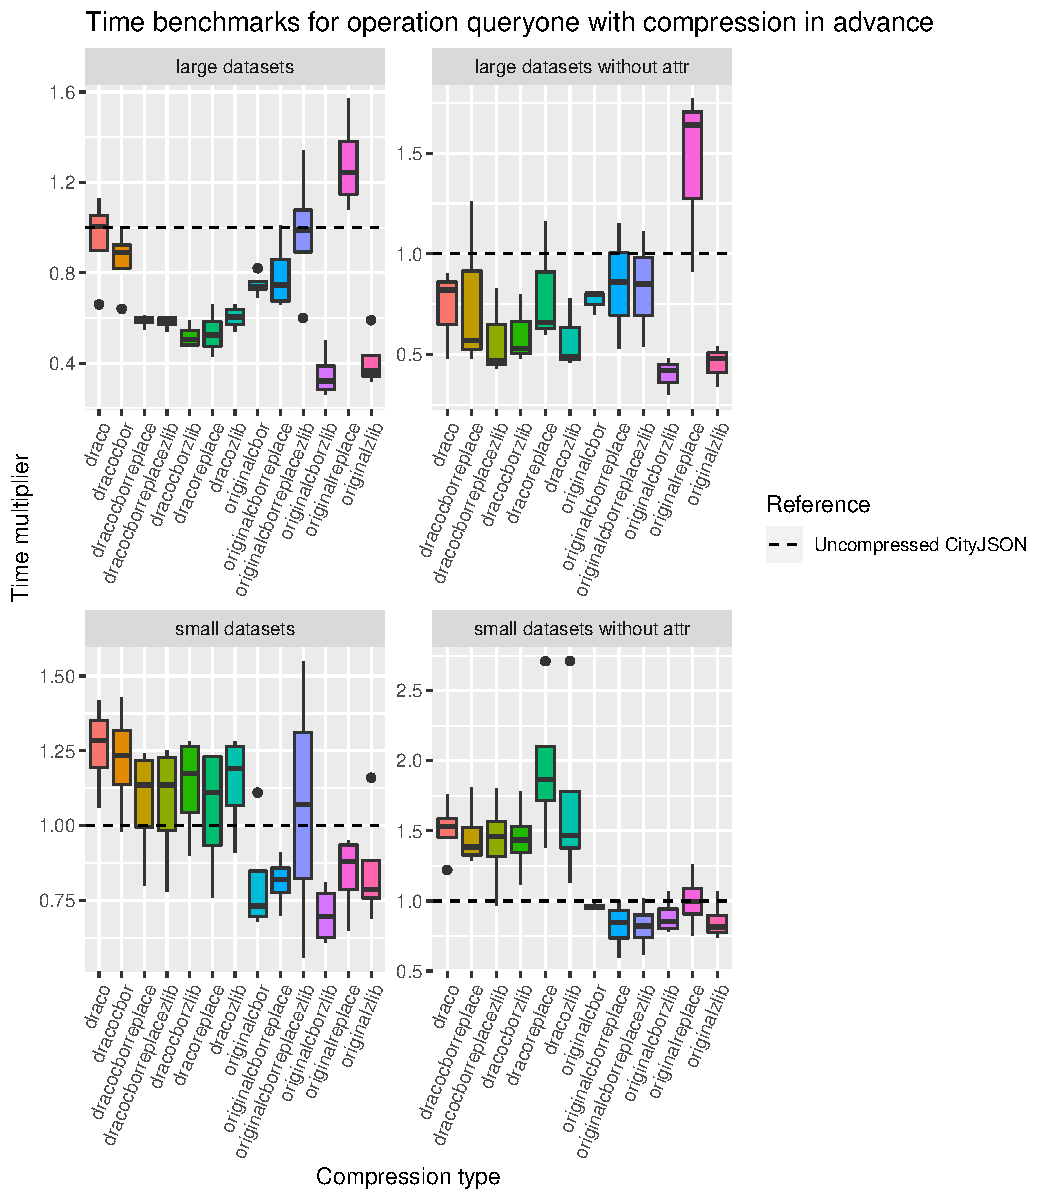
\includegraphics[scale=0.92]{figs/benchmark/individual/queryone.pdf}
    \caption{Boxplots of time performance of (in advance) compressed datasets on querying one feature compared to uncompressed CityJSON.}
    \label{fig:sdvis}
\end{figure}

With the large datasets, most compression types have good performance, especially when datasets do have attributes.
Compression types with original geometries and using the replace method do not do well, and this would be due to only one city object having to be compressed, which does not have a lot of repeated parts in it.
Draco compression is not clearly better or worse.
Original-cbor-zlib and original-zlib do espcially well with this use case, indicating that they have a good balance between file size compression and decoding time.

With the small datasets using Draco yields worse performance.
This is not expected when comparing it to the results of the large datasets, as in both cases only one city object has to be compressed.
Without using Draco compression beneficial results can be achieved.
There are no clear differences between having attributes or not, except for the results of original-cbor-replace-zlib having a large spread which I can not explain.

Compression in advance can improve the querying time of CityJSON datasets on one city object to 32\%, 42\%, 69\%, or 81\% (when respectively using large datasets, large datasets without attributes, small datasets, and small datasets without attributes) of the time that it takes to perform the same operation with uncompressed CityJSON.


  \begin{table}[!h]
    \begin{minipage}{.5\linewidth}
      \caption{
Median performance with queryone on large datasets, compression in advance}
\centering

\begin{tabular}{|l|r|}
\hline
Compression type & median\\
\hline
originalcborzlib & 0.320\\
\hline
originalzlib & 0.365\\
\hline
dracocborzlib & 0.505\\
\hline
dracoreplace & 0.525\\
\hline
dracocborreplacezlib & 0.590\\
\hline
dracocborreplace & 0.595\\
\hline
dracozlib & 0.605\\
\hline
originalcbor & 0.740\\
\hline
originalcborreplace & 0.745\\
\hline
dracocbor & 0.890\\
\hline
originalcborreplacezlib & 0.990\\
\hline
draco & 1.005\\
\hline
originalreplace & 1.245\\
\hline
\end{tabular}
\end{minipage}%
    \begin{minipage}{.5\linewidth}
      \centering
        \caption{
Median performance with queryone on large datasets without attributes, compression in advance}

\begin{tabular}{|l|r|}
\hline
Compression type & median\\
\hline
originalcborzlib & 0.42\\
\hline
dracocborreplacezlib & 0.47\\
\hline
originalzlib & 0.48\\
\hline
dracozlib & 0.49\\
\hline
dracocborzlib & 0.53\\
\hline
dracocborreplace & 0.57\\
\hline
dracoreplace & 0.66\\
\hline
originalcbor & 0.80\\
\hline
draco & 0.82\\
\hline
originalcborreplacezlib & 0.85\\
\hline
originalcborreplace & 0.86\\
\hline
originalreplace & 1.64\\
\hline
\end{tabular}
\end{minipage} 
\end{table}
\begin{table}[!h]
    \begin{minipage}{.5\linewidth}
      \caption{
Median performance with queryone on small datasets, compression in advance}
\centering

\begin{tabular}{|l|r|}
\hline
Compression type & median\\
\hline
originalcborzlib & 0.695\\
\hline
originalcbor & 0.730\\
\hline
originalzlib & 0.785\\
\hline
originalcborreplace & 0.820\\
\hline
originalreplace & 0.880\\
\hline
originalcborreplacezlib & 1.070\\
\hline
dracoreplace & 1.110\\
\hline
dracocborreplace & 1.135\\
\hline
dracocborreplacezlib & 1.135\\
\hline
dracocborzlib & 1.175\\
\hline
dracozlib & 1.190\\
\hline
dracocbor & 1.235\\
\hline
draco & 1.285\\
\hline
\end{tabular}
\end{minipage}%
    \begin{minipage}{.5\linewidth}
      \centering
        \caption{
Median performance with queryone on small datasets without attributes, compression in advance}

\begin{tabular}{|l|r|}
\hline
Compression type & median\\
\hline
originalzlib & 0.815\\
\hline
originalcborreplacezlib & 0.820\\
\hline
originalcborreplace & 0.845\\
\hline
originalcborzlib & 0.855\\
\hline
originalcbor & 0.955\\
\hline
originalreplace & 0.995\\
\hline
dracocborreplace & 1.385\\
\hline
dracocborzlib & 1.435\\
\hline
dracocborreplacezlib & 1.460\\
\hline
dracozlib & 1.465\\
\hline
draco & 1.530\\
\hline
dracoreplace & 1.865\\
\hline
\end{tabular}
\end{minipage} 
\end{table}


\subsubsection{Compression on the fly}

\begin{figure}[h!]
    %\hspace*{-2.3cm}  
    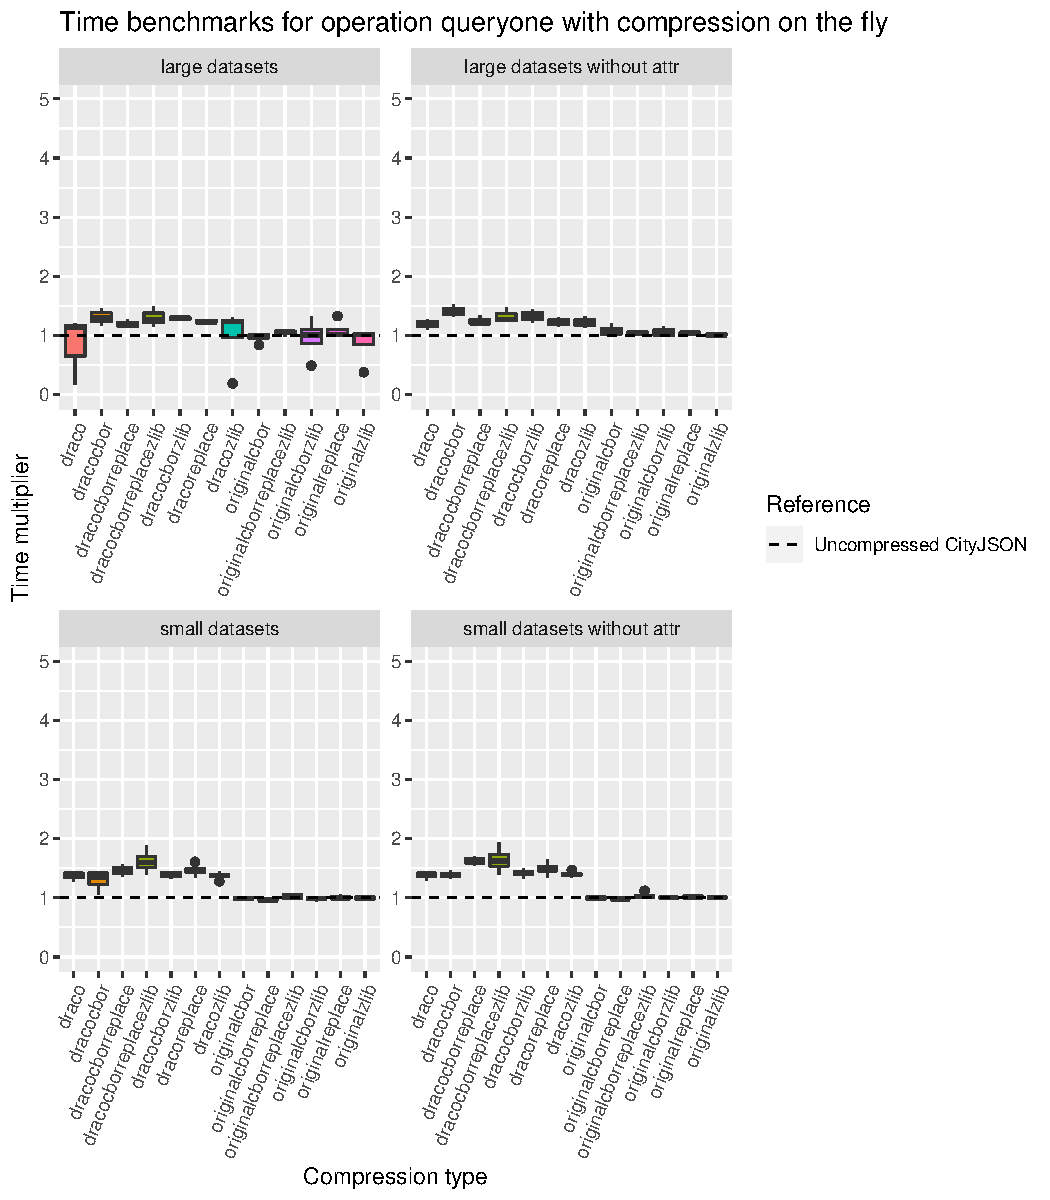
\includegraphics[scale=0.92]{figs/benchmark/individualotf/queryone.pdf}
    \caption{Boxplots of time performance of (on the fly) compressed datasets on querying one feature compared to uncompressed CityJSON.}
    \label{figotf:sdvis}
\end{figure}

For this use case, Draco compression is detrimental for performance.
Compression time is added into it and this is not worth it when compressing only one city object.
Other compression types are also often not worth it, especially on the large datasets, regardless of attributes.
With the small datasets, only original-cbor-replace works well with both dataset types.
One city object would not have much redundancy to compress and is already slim, so compression is not useful here and might even give slower performance.

On the fly compression can improve the querying time of CityJSON datasets on one city object to 100\%, 100\%, 96\%, or 98\% (when respectively using large datasets, large datasets without attributes, small datasets, and small datasets without attributes) of the time that it takes to perform the same operation with uncompressed CityJSON.


  \begin{table}[!h]
    \begin{minipage}{.5\linewidth}
      \caption{
Median performance with queryone on large datasets, compression on the fly}
\centering

\begin{tabular}{|l|r|}
\hline
Compression type & median\\
\hline
originalcbor & 1.005\\
\hline
originalcborzlib & 1.010\\
\hline
originalzlib & 1.015\\
\hline
originalreplace & 1.020\\
\hline
originalcborreplacezlib & 1.070\\
\hline
draco & 1.140\\
\hline
dracocborreplace & 1.180\\
\hline
dracoreplace & 1.230\\
\hline
dracozlib & 1.235\\
\hline
dracocborreplacezlib & 1.270\\
\hline
dracocborzlib & 1.300\\
\hline
dracocbor & 1.310\\
\hline
\end{tabular}
\end{minipage}%
    \begin{minipage}{.5\linewidth}
      \centering
        \caption{
Median performance with queryone on large datasets without attributes, compression on the fly}

\begin{tabular}{|l|r|}
\hline
Compression type & median\\
\hline
originalzlib & 1.010\\
\hline
originalcborzlib & 1.030\\
\hline
originalcborreplacezlib & 1.040\\
\hline
originalreplace & 1.040\\
\hline
originalcbor & 1.050\\
\hline
draco & 1.195\\
\hline
dracocborreplace & 1.210\\
\hline
dracoreplace & 1.220\\
\hline
dracozlib & 1.220\\
\hline
dracocborreplacezlib & 1.270\\
\hline
dracocborzlib & 1.330\\
\hline
dracocbor & 1.390\\
\hline
\end{tabular}
\end{minipage} 
\end{table}
\begin{table}[!h]
    \begin{minipage}{.5\linewidth}
      \caption{
Median performance with queryone on small datasets, compression on the fly}
\centering

\begin{tabular}{|l|r|}
\hline
Compression type & median\\
\hline
originalcborreplace & 0.960\\
\hline
originalcbor & 0.985\\
\hline
originalcborzlib & 0.990\\
\hline
originalzlib & 0.995\\
\hline
originalreplace & 1.000\\
\hline
originalcborreplacezlib & 1.020\\
\hline
dracocbor & 1.355\\
\hline
dracozlib & 1.380\\
\hline
draco & 1.400\\
\hline
dracocborzlib & 1.400\\
\hline
dracoreplace & 1.455\\
\hline
dracocborreplace & 1.460\\
\hline
dracocborreplacezlib & 1.595\\
\hline
\end{tabular}
\end{minipage}%
    \begin{minipage}{.5\linewidth}
      \centering
        \caption{
Median performance with queryone on small datasets without attributes, compression on the fly}

\begin{tabular}{|l|r|}
\hline
Compression type & median\\
\hline
originalcborreplace & 0.980\\
\hline
originalcbor & 1.000\\
\hline
originalcborzlib & 1.005\\
\hline
originalzlib & 1.005\\
\hline
originalreplace & 1.015\\
\hline
originalcborreplacezlib & 1.020\\
\hline
dracocbor & 1.390\\
\hline
dracozlib & 1.390\\
\hline
draco & 1.410\\
\hline
dracocborzlib & 1.425\\
\hline
dracoreplace & 1.495\\
\hline
dracocborreplace & 1.625\\
\hline
dracocborreplacezlib & 1.625\\
\hline
\end{tabular}
\end{minipage} 
\end{table}





\subsection{Querying all features}

\subsubsection{Compression in advance}

\begin{figure}[h!]
    %\hspace*{-2.3cm}  
    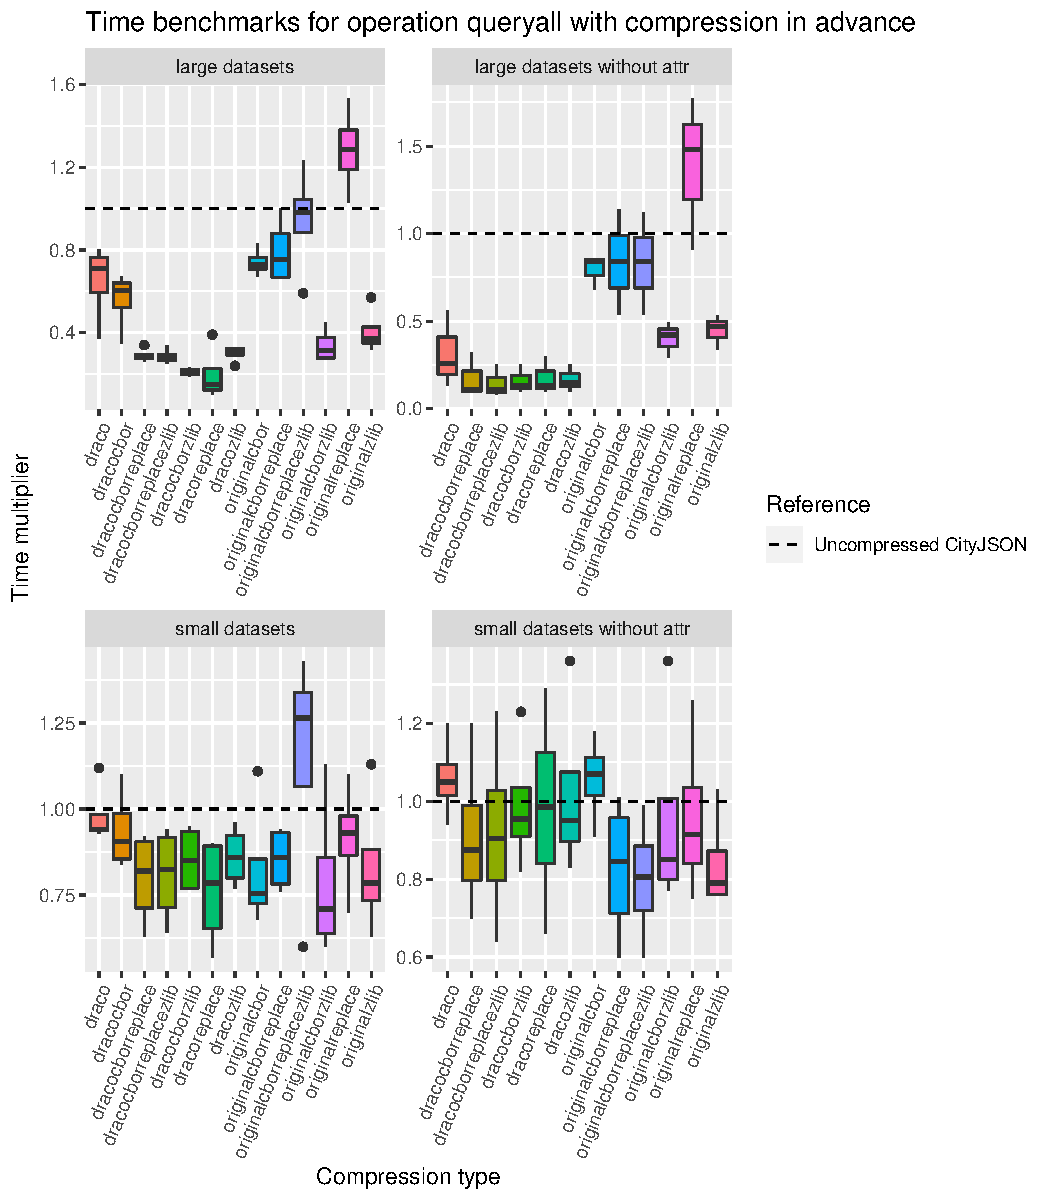
\includegraphics[scale=0.92]{figs/benchmark/individual/queryall.pdf}
    \caption{Boxplots of time performance of (in advance) compressed datasets on querying all features compared to uncompressed CityJSON.}
    \label{fig:sdvis}
\end{figure}

When querying all city objects, the whole dataset is traversed but the compression is performed on the complete file in the end.
With large datasets, using Draco is beneficial compared to compression types that do not use it.
This is likely due to Draco geometries being queried in a different way, as explained in Section~\ref{sec:queryone}.
However, original-cbor-zlib and original-zlib are also good, and are better than using draco alone or draco-cbor with datasets that have attributes.

As for the small datasets, Draco again provides less added benefits as is generally the case when datasets are compressed beforehand.
There is no clear pattern to be noted when comparing compression types to each other.
But as seen before as well, using cbor, zlib, or combinations of these prove to do well.

Compression in advance can improve the querying time of CityJSON datasets on all city objects to 15\%, 11\%, 71\%, or 79\% (when respectively using large datasets, large datasets without attributes, small datasets, and small datasets without attributes) of the time that it takes to perform the same operation with uncompressed CityJSON.



  \begin{table}[!h]
    \begin{minipage}{.5\linewidth}
      \caption{
Median performance with queryall on large datasets, compression in advance}
\centering

\begin{tabular}{|l|r|}
\hline
Compression type & median\\
\hline
dracoreplace & 0.150\\
\hline
dracocborzlib & 0.210\\
\hline
dracocborreplacezlib & 0.275\\
\hline
dracocborreplace & 0.280\\
\hline
dracozlib & 0.315\\
\hline
originalcborzlib & 0.315\\
\hline
originalzlib & 0.370\\
\hline
dracocbor & 0.605\\
\hline
draco & 0.710\\
\hline
originalcbor & 0.730\\
\hline
originalcborreplace & 0.755\\
\hline
originalcborreplacezlib & 0.980\\
\hline
originalreplace & 1.285\\
\hline
\end{tabular}
\end{minipage}%
    \begin{minipage}{.5\linewidth}
      \centering
        \caption{
Median performance with queryall on large datasets without attributes, compression in advance}

\begin{tabular}{|l|r|}
\hline
Compression type & median\\
\hline
dracocborreplace & 0.11\\
\hline
dracocborreplacezlib & 0.11\\
\hline
dracocborzlib & 0.13\\
\hline
dracoreplace & 0.13\\
\hline
dracozlib & 0.15\\
\hline
draco & 0.26\\
\hline
originalcborzlib & 0.42\\
\hline
originalzlib & 0.47\\
\hline
originalcbor & 0.84\\
\hline
originalcborreplace & 0.84\\
\hline
originalcborreplacezlib & 0.84\\
\hline
originalreplace & 1.48\\
\hline
\end{tabular}
\end{minipage} 
\end{table}
\begin{table}[!h]
    \begin{minipage}{.5\linewidth}
      \caption{
Median performance with queryall on small datasets, compression in advance}
\centering

\begin{tabular}{|l|r|}
\hline
Compression type & median\\
\hline
originalcborzlib & 0.710\\
\hline
originalcbor & 0.755\\
\hline
dracoreplace & 0.785\\
\hline
originalzlib & 0.785\\
\hline
dracocborreplace & 0.820\\
\hline
dracocborreplacezlib & 0.825\\
\hline
dracocborzlib & 0.850\\
\hline
dracozlib & 0.860\\
\hline
originalcborreplace & 0.860\\
\hline
dracocbor & 0.905\\
\hline
originalreplace & 0.930\\
\hline
draco & 0.940\\
\hline
originalcborreplacezlib & 1.265\\
\hline
\end{tabular}
\end{minipage}%
    \begin{minipage}{.5\linewidth}
      \centering
        \caption{
Median performance with queryall on small datasets without attributes, compression in advance}

\begin{tabular}{|l|r|}
\hline
Compression type & median\\
\hline
originalzlib & 0.790\\
\hline
originalcborreplacezlib & 0.805\\
\hline
originalcborreplace & 0.845\\
\hline
originalcborzlib & 0.850\\
\hline
dracocborreplace & 0.875\\
\hline
dracocborreplacezlib & 0.905\\
\hline
originalreplace & 0.915\\
\hline
dracozlib & 0.950\\
\hline
dracocborzlib & 0.955\\
\hline
dracoreplace & 0.985\\
\hline
draco & 1.050\\
\hline
originalcbor & 1.070\\
\hline
\end{tabular}
\end{minipage} 
\end{table}

\clearpage

\subsubsection{Compression on the fly}

\begin{figure}[h!]
    %\hspace*{-2.3cm}  
    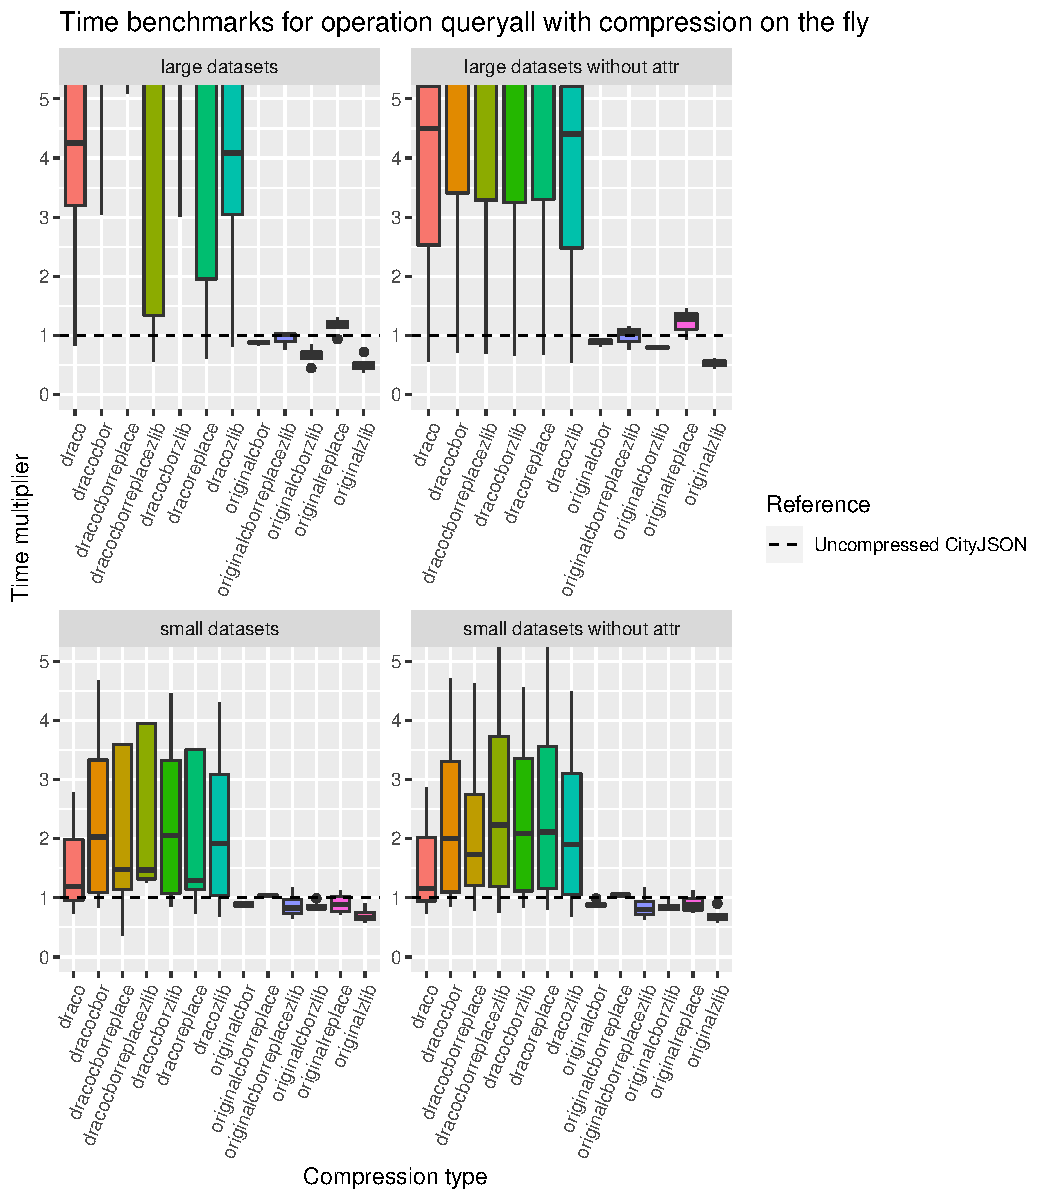
\includegraphics[scale=0.92]{figs/benchmark/individualotf/queryall.pdf}
    \caption{Boxplots of time performance of (on the fly) compressed datasets on querying all features compared to uncompressed CityJSON.}
    \label{figotf:sdvis}
\end{figure}

The graphs are limited by a time multiplier of 5.
Again, using Draco is not a good idea when compressing datasets on the fly because of the relatively high compression time.
Original-replace is unsuitable with large datasets, and original-cbor-replace-zlib also does not do very well.
Original-zlib and original-cbor-zlib are the best ones, both with and without attributes.
As for the small datasets these two are also good, but using the replace method is now not noticeably worse.

On the fly compression can improve the querying time of CityJSON datasets on all city objects to 47\%, 53\%, 67\%, or 65\% (when respectively using large datasets, large datasets without attributes, small datasets, and small datasets without attributes) of the time that it takes to perform the same operation with uncompressed CityJSON.


\begin{table}[!h]
    \begin{minipage}{.5\linewidth}
      \caption{
Median performance with queryall on large datasets, compression on the fly}
\centering

\begin{tabular}{|l|r|}
\hline
Compression type & median\\
\hline
originalzlib & 0.470\\
\hline
originalcborzlib & 0.675\\
\hline
originalcbor & 0.885\\
\hline
originalcborreplacezlib & 1.020\\
\hline
originalreplace & 1.205\\
\hline
dracozlib & 4.085\\
\hline
draco & 4.255\\
\hline
dracoreplace & 6.125\\
\hline
dracocborreplacezlib & 6.340\\
\hline
dracocborzlib & 7.465\\
\hline
dracocbor & 9.835\\
\hline
dracocborreplace & 13.260\\
\hline
\end{tabular}
\end{minipage}%
    \begin{minipage}{.5\linewidth}
      \centering
        \caption{
Median performance with queryall on large datasets without attributes, compression on the fly}

\begin{tabular}{|l|r|}
\hline
Compression type & median\\
\hline
originalzlib & 0.53\\
\hline
originalcborzlib & 0.80\\
\hline
originalcbor & 0.91\\
\hline
originalcborreplacezlib & 1.04\\
\hline
originalreplace & 1.28\\
\hline
dracozlib & 4.41\\
\hline
draco & 4.50\\
\hline
dracocborzlib & 5.82\\
\hline
dracocborreplacezlib & 5.88\\
\hline
dracoreplace & 5.93\\
\hline
dracocbor & 6.11\\
\hline
\end{tabular}
\end{minipage} 
\end{table}
\begin{table}[!h]
    \begin{minipage}{.5\linewidth}
      \caption{
Median performance with queryall on small datasets, compression on the fly}
\centering

\begin{tabular}{|l|r|}
\hline
Compression type & median\\
\hline
originalzlib & 0.670\\
\hline
originalcborzlib & 0.820\\
\hline
originalcborreplacezlib & 0.830\\
\hline
originalcbor & 0.890\\
\hline
originalreplace & 0.890\\
\hline
originalcborreplace & 1.040\\
\hline
draco & 1.190\\
\hline
dracoreplace & 1.290\\
\hline
dracocborreplacezlib & 1.470\\
\hline
dracocborreplace & 1.475\\
\hline
dracozlib & 1.920\\
\hline
dracocbor & 2.030\\
\hline
dracocborzlib & 2.050\\
\hline
\end{tabular}
\end{minipage}%     
    \begin{minipage}{.5\linewidth}
      \centering
        \caption{
Median performance with queryall on small datasets without attributes, compression on the fly}

\begin{tabular}{|l|r|}
\hline
Compression type & median\\
\hline
originalzlib & 0.650\\
\hline
originalcborreplacezlib & 0.805\\
\hline
originalcborzlib & 0.820\\
\hline
originalcbor & 0.870\\
\hline
originalreplace & 0.880\\
\hline
originalcborreplace & 1.050\\
\hline
draco & 1.160\\
\hline
dracocborreplace & 1.735\\
\hline
dracozlib & 1.905\\
\hline
dracocbor & 2.005\\
\hline
dracocborzlib & 2.085\\
\hline
dracoreplace & 2.115\\
\hline
dracocborreplacezlib & 2.230\\
\hline
\end{tabular}
\end{minipage} 
\end{table}

\newpage

\section{Spatial analysis}
\label{bmbuffering}

\subsection{Buffering one feature}


\subsubsection{Compression in advance}

\begin{figure}[h!]
    %\hspace*{-2.3cm}  
    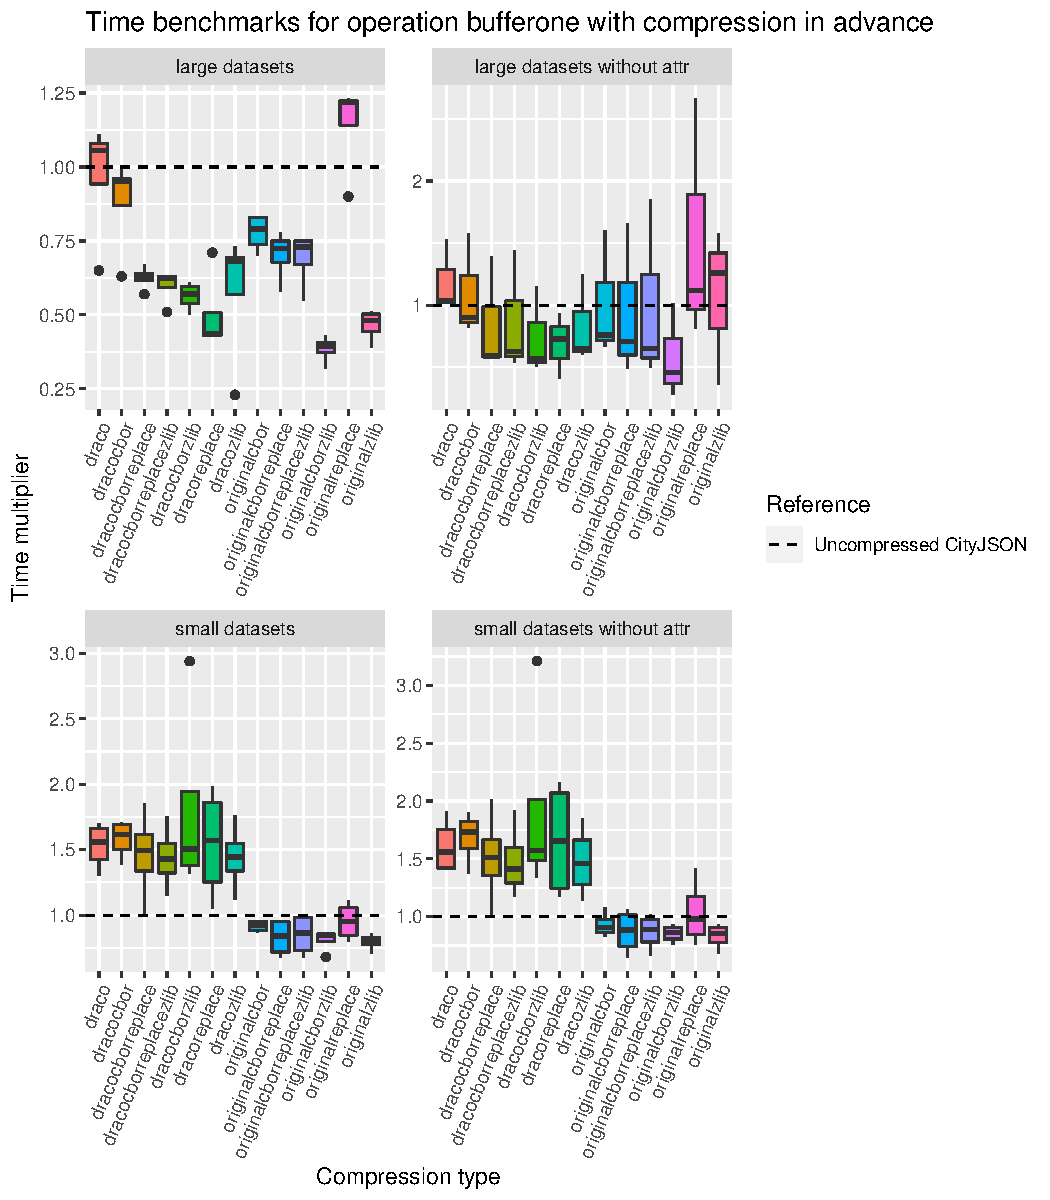
\includegraphics[scale=0.92]{figs/benchmark/individual/bufferone.pdf}
    \caption{Boxplots of time performance of (in advance) compressed datasets on buffering one feature compared to uncompressed CityJSON.}
    \label{fig:sdvis}
\end{figure}

Draco geometries are handled in a different way than original geometries as explained in Section~\ref{sec:implbufferone}.
Despite that, for the large datasets it is not easy to see whether it is better to use it or not.
There are also no clear rends to be seen, except for that original-replace is bad both with and without attributes, and original-cbor-zlib is the best option for both of these dataset types.
In general, most compression types work well with large datasets with attributes but not as good when attributes are not included.
In the latter case both attribute and JSON compression techniques have less data to compress, which might make them less effective.
Regarding the small datasets, the use of Draco gives worse results than not using it due to overhead.
The other compression types general do well as compared to the baseline, except for original-replace.

Compression in advance can improve the buffering time of CityJSON datasets on one city object to 39\%, 46\%, 81\%, or 85\% (when respectively using large datasets, large datasets without attributes, small datasets, and small datasets without attributes) of the time that it takes to perform the same operation with uncompressed CityJSON.



  \begin{table}[!h]
    \begin{minipage}{.5\linewidth}
      \caption{
Median performance with bufferone on large datasets, compression in advance}
\centering

\begin{tabular}{|l|r|}
\hline
Compression type & median\\
\hline
originalcborzlib & 0.395\\
\hline
dracoreplace & 0.435\\
\hline
originalzlib & 0.480\\
\hline
dracocborzlib & 0.570\\
\hline
dracocborreplacezlib & 0.625\\
\hline
dracocborreplace & 0.630\\
\hline
dracozlib & 0.680\\
\hline
originalcborreplace & 0.725\\
\hline
originalcborreplacezlib & 0.730\\
\hline
originalcbor & 0.790\\
\hline
dracocbor & 0.950\\
\hline
draco & 1.055\\
\hline
originalreplace & 1.220\\
\hline
\end{tabular}
\end{minipage}%
    \begin{minipage}{.5\linewidth}
      \centering
        \caption{
Median performance with bufferone on large datasets without attributes, compression in advance}

\begin{tabular}{|l|r|}
\hline
Compression type & median\\
\hline
originalcborzlib & 0.46\\
\hline
dracocborzlib & 0.57\\
\hline
dracocborreplace & 0.59\\
\hline
dracocborreplacezlib & 0.63\\
\hline
dracozlib & 0.65\\
\hline
originalcborreplacezlib & 0.65\\
\hline
originalcborreplace & 0.71\\
\hline
dracoreplace & 0.73\\
\hline
originalcbor & 0.76\\
\hline
dracocbor & 0.90\\
\hline
draco & 1.04\\
\hline
originalreplace & 1.12\\
\hline
originalzlib & 1.26\\
\hline
\end{tabular}
\end{minipage} 
\end{table}
\begin{table}[!h]
    \begin{minipage}{.5\linewidth}
      \caption{
Median performance with bufferone on small datasets, compression in advance}
\centering

\begin{tabular}{|l|r|}
\hline
Compression type & median\\
\hline
originalzlib & 0.810\\
\hline
originalcborreplace & 0.840\\
\hline
originalcborzlib & 0.845\\
\hline
originalcborreplacezlib & 0.865\\
\hline
originalcbor & 0.920\\
\hline
originalreplace & 0.950\\
\hline
dracocborreplacezlib & 1.430\\
\hline
dracozlib & 1.445\\
\hline
dracocborreplace & 1.495\\
\hline
dracocborzlib & 1.505\\
\hline
draco & 1.560\\
\hline
dracoreplace & 1.570\\
\hline
dracocbor & 1.615\\
\hline
\end{tabular}
\end{minipage}%
    \begin{minipage}{.5\linewidth}
      \centering
        \caption{
Median performance with bufferone on small datasets without attributes, compression in advance}

\begin{tabular}{|l|r|}
\hline
Compression type & median\\
\hline
originalzlib & 0.855\\
\hline
originalcborzlib & 0.860\\
\hline
originalcborreplace & 0.885\\
\hline
originalcborreplacezlib & 0.890\\
\hline
originalcbor & 0.905\\
\hline
originalreplace & 0.980\\
\hline
dracocborreplacezlib & 1.410\\
\hline
dracozlib & 1.460\\
\hline
dracocborreplace & 1.510\\
\hline
draco & 1.560\\
\hline
dracocborzlib & 1.570\\
\hline
dracoreplace & 1.655\\
\hline
dracocbor & 1.730\\
\hline
\end{tabular}
\end{minipage} 
\end{table}



\subsubsection{Compression on the fly}

\begin{figure}[h!]
    %\hspace*{-2.3cm}  
    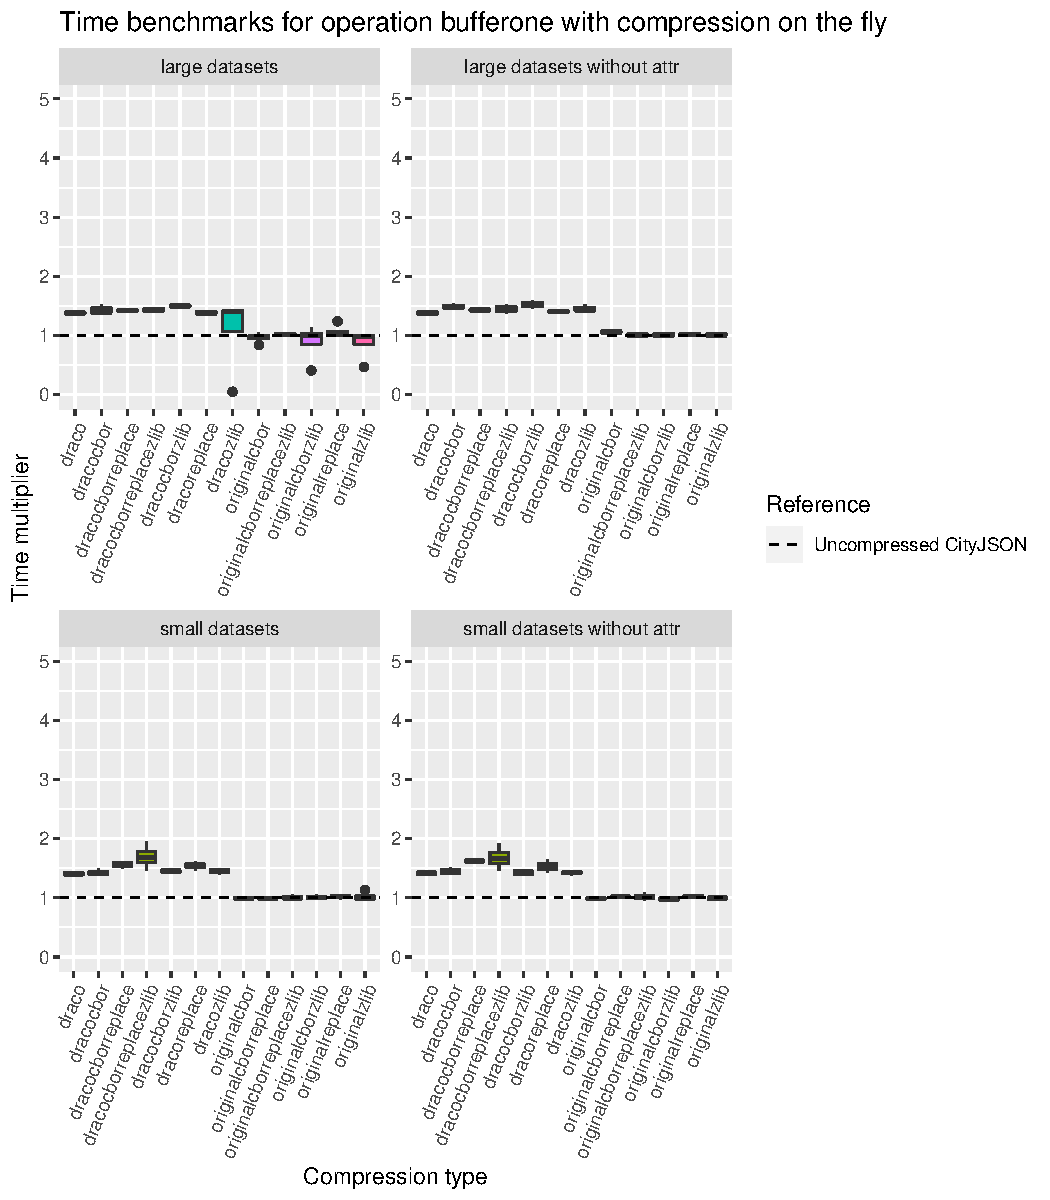
\includegraphics[scale=0.92]{figs/benchmark/individualotf/bufferone.pdf}
    \caption{Boxplots of time performance of (on the fly) compressed datasets on buffering one feature compared to uncompressed CityJSON.}
    \label{figotf:sdvis}
\end{figure}

As opposed to compressing in advance, it is almost never worth it to compress buffer data on the fly since the medians of the boxplots are above the baseline or very slightly underneath it.
This means that the added compression time is not outweighed by the faster transmission of the data.
Especially when using Draco this is true.
When using a compression type that retains original geometries, the results can be neutral so it is at least still fine to implement such kind of compression.

On the fly compression can improve the buffering time of CityJSON datasets on one city object to 98\%, 100\%, 99\%, or 98\% (when respectively using large datasets, large datasets without attributes, small datasets, and small datasets without attributes) of the time that it takes to perform the same operation with uncompressed CityJSON.


  \begin{table}[!h]
    \begin{minipage}{.5\linewidth}
      \caption{
Median performance with bufferone on large datasets, compression on the fly}
\centering

\begin{tabular}{|l|r|}
\hline
Compression type & median\\
\hline
originalcbor & 0.980\\
\hline
originalzlib & 0.985\\
\hline
originalcborzlib & 1.000\\
\hline
originalreplace & 1.015\\
\hline
originalcborreplacezlib & 1.020\\
\hline
draco & 1.380\\
\hline
dracoreplace & 1.380\\
\hline
dracocbor & 1.400\\
\hline
dracozlib & 1.410\\
\hline
dracocborreplace & 1.420\\
\hline
dracocborreplacezlib & 1.430\\
\hline
dracocborzlib & 1.500\\
\hline
\end{tabular}
\end{minipage}%
    \begin{minipage}{.5\linewidth}
      \centering
        \caption{
Median performance with bufferone on large datasets without attributes, compression on the fly}

\begin{tabular}{|l|r|}
\hline
Compression type & median\\
\hline
originalcborzlib & 1.000\\
\hline
originalcborreplacezlib & 1.010\\
\hline
originalzlib & 1.010\\
\hline
originalreplace & 1.020\\
\hline
originalcbor & 1.060\\
\hline
draco & 1.385\\
\hline
dracoreplace & 1.410\\
\hline
dracocborreplace & 1.430\\
\hline
dracozlib & 1.430\\
\hline
dracocborreplacezlib & 1.440\\
\hline
dracocbor & 1.480\\
\hline
dracocborzlib & 1.520\\
\hline
\end{tabular}
\end{minipage} 
\end{table}
\begin{table}[!h]
    \begin{minipage}{.5\linewidth}
      \caption{
Median performance with bufferone on small datasets, compression on the fly}
\centering

\begin{tabular}{|l|r|}
\hline
Compression type & median\\
\hline
originalcbor & 0.990\\
\hline
originalcborreplace & 0.990\\
\hline
originalzlib & 0.995\\
\hline
originalcborreplacezlib & 1.000\\
\hline
originalcborzlib & 1.005\\
\hline
originalreplace & 1.025\\
\hline
draco & 1.400\\
\hline
dracocbor & 1.415\\
\hline
dracocborzlib & 1.450\\
\hline
dracozlib & 1.455\\
\hline
dracoreplace & 1.545\\
\hline
dracocborreplace & 1.560\\
\hline
dracocborreplacezlib & 1.680\\
\hline
\end{tabular}
\end{minipage}%       
    \begin{minipage}{.5\linewidth}
      \centering
        \caption{
Median performance with bufferone on small datasets without attributes, compression on the fly}

\begin{tabular}{|l|r|}
\hline
Compression type & median\\
\hline
originalcborzlib & 0.980\\
\hline
originalcbor & 0.985\\
\hline
originalzlib & 0.995\\
\hline
originalcborreplacezlib & 1.005\\
\hline
originalcborreplace & 1.020\\
\hline
originalreplace & 1.020\\
\hline
draco & 1.420\\
\hline
dracocborzlib & 1.425\\
\hline
dracozlib & 1.425\\
\hline
dracocbor & 1.440\\
\hline
dracoreplace & 1.525\\
\hline
dracocborreplace & 1.625\\
\hline
dracocborreplacezlib & 1.665\\
\hline
\end{tabular}
\end{minipage} 
\end{table}

\newpage

\subsection{Buffering all features}
\label{resultsbufferall}

\subsubsection{Compression in advance}

\begin{figure}[h!]
    %\hspace*{-2.3cm}  
    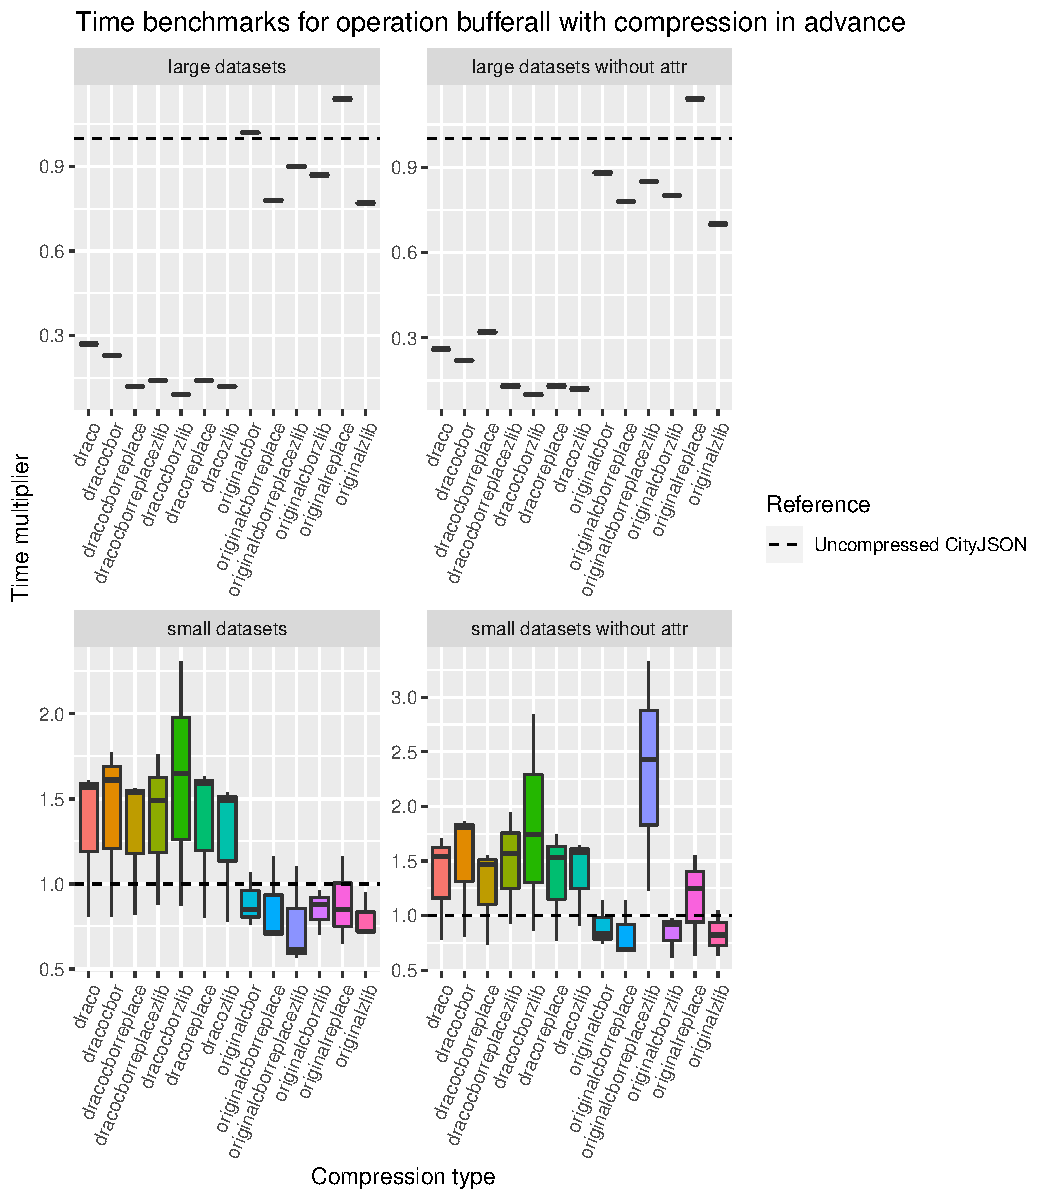
\includegraphics[scale=0.92]{figs/benchmark/individual/bufferall.pdf}
    \caption{Boxplots of time performance of (in advance) compressed datasets on buffering all features compared to uncompressed CityJSON.}
    \label{fig:sdvis}
\end{figure}

When buffering all features in the client, using Draco is clearly a good idea for the large datasets.
Draco geometries are buffered in a different way (see Section~\ref{sec:implbufferone}), and this shows a more apparent advantage when all geometries are buffered instead of one.
Compression types without it generally still improve the performance in comparison to the baseline, but not as much.
For small datasets these perform better however, which is also seen with the other use cases with small datasets.
Draco is again unsuitable to use with those.
But ultimately, it is questionable whether or not it is wise to use compression at all for this use case, since the boxplots show that most compression types that have a median below the baseline still have their boxplots touching or above the baseline.

Compression in advance can improve the buffering time of CityJSON datasets on all city objects to 9\%, 10\%, 61\%, or 69\% (when respectively using large datasets, large datasets without attributes, small datasets, and small datasets without attributes) of the time that it takes to perform the same operation with uncompressed CityJSON.



  \begin{table}[!h]
    \begin{minipage}{.5\linewidth}
      \caption{
Median performance with bufferall on large datasets, compression in advance}
\centering

\begin{tabular}{|l|r|}
\hline
Compression type & median\\
\hline
dracocborzlib & 0.09\\
\hline
dracocborreplace & 0.12\\
\hline
dracozlib & 0.12\\
\hline
dracocborreplacezlib & 0.14\\
\hline
dracoreplace & 0.14\\
\hline
dracocbor & 0.23\\
\hline
draco & 0.27\\
\hline
originalzlib & 0.77\\
\hline
originalcborreplace & 0.78\\
\hline
originalcborzlib & 0.87\\
\hline
originalcborreplacezlib & 0.90\\
\hline
originalcbor & 1.02\\
\hline
originalreplace & 1.14\\
\hline
\end{tabular}
\end{minipage}%
    \begin{minipage}{.5\linewidth}
      \centering
        \caption{
Median performance with bufferall on large datasets without attributes, compression in advance}

\begin{tabular}{|l|r|}
\hline
Compression type & median\\
\hline
dracocborzlib & 0.10\\
\hline
dracozlib & 0.12\\
\hline
dracocborreplacezlib & 0.13\\
\hline
dracoreplace & 0.13\\
\hline
dracocbor & 0.22\\
\hline
draco & 0.26\\
\hline
dracocborreplace & 0.32\\
\hline
originalzlib & 0.70\\
\hline
originalcborreplace & 0.78\\
\hline
originalcborzlib & 0.80\\
\hline
originalcborreplacezlib & 0.85\\
\hline
originalcbor & 0.88\\
\hline
originalreplace & 1.14\\
\hline
\end{tabular}
\end{minipage} 
\end{table}
\begin{table}[!h]
    \begin{minipage}{.5\linewidth}
      \caption{
Median performance with bufferall on small datasets, compression in advance}
\centering

\begin{tabular}{|l|r|}
\hline
Compression type & median\\
\hline
originalcborreplacezlib & 0.61\\
\hline
originalcborreplace & 0.71\\
\hline
originalzlib & 0.72\\
\hline
originalcbor & 0.85\\
\hline
originalreplace & 0.85\\
\hline
originalcborzlib & 0.88\\
\hline
dracocborreplacezlib & 1.49\\
\hline
dracozlib & 1.49\\
\hline
dracocborreplace & 1.54\\
\hline
draco & 1.57\\
\hline
dracoreplace & 1.59\\
\hline
dracocbor & 1.61\\
\hline
dracocborzlib & 1.65\\
\hline
\end{tabular}
\end{minipage}%
    \begin{minipage}{.5\linewidth}
      \centering
        \caption{
Median performance with bufferall on small datasets without attributes, compression in advance}

\begin{tabular}{|l|r|}
\hline
Compression type & median\\
\hline
originalcborreplace & 0.69\\
\hline
originalzlib & 0.82\\
\hline
originalcbor & 0.83\\
\hline
originalcborzlib & 0.92\\
\hline
originalreplace & 1.25\\
\hline
dracocborreplace & 1.47\\
\hline
dracoreplace & 1.53\\
\hline
draco & 1.54\\
\hline
dracocborreplacezlib & 1.57\\
\hline
dracozlib & 1.58\\
\hline
dracocborzlib & 1.74\\
\hline
dracocbor & 1.81\\
\hline
originalcborreplacezlib & 2.43\\
\hline
\end{tabular}
\end{minipage} 
\end{table}

\clearpage

\subsubsection{Compression on the fly}

\begin{figure}[h!]
    %\hspace*{-2.3cm}  
    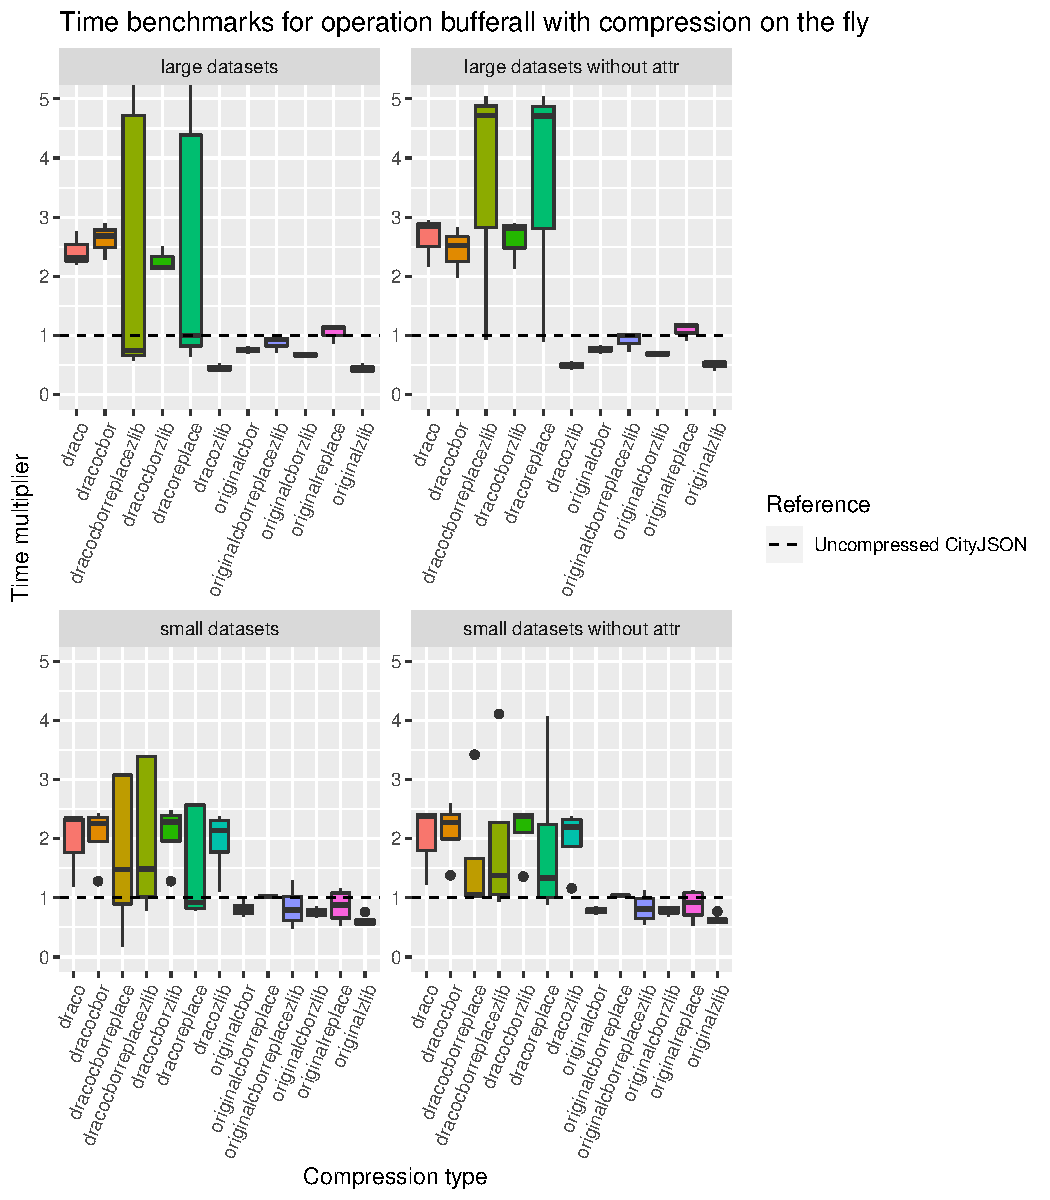
\includegraphics[scale=0.92]{figs/benchmark/individualotf/bufferall.pdf}
    \caption{Boxplots of time performance of (on the fly) compressed datasets on buffering all features compared to uncompressed CityJSON.}
    \label{figotf:sdvis}
\end{figure}

Using Draco compression on the fly is not useful.
Other compression types on the other hand do provide benefits, except when the replace method is used.
This is true for all dataset types, and there are no other interesting patterns to see in the graphs.


On the fly compression can improve the buffering time of CityJSON datasets on all city objects to 41\%, 50\%, 57\%, or 60\% (when respectively using large datasets, large datasets without attributes, small datasets, and small datasets without attributes) of the time that it takes to perform the same operation with uncompressed CityJSON.


\begin{table}[!h]
    \begin{minipage}{.5\linewidth}
      \caption{
Median performance with bufferall on large datasets, compression on the fly}
\centering

\begin{tabular}{|l|r|}
\hline
Compression type & median\\
\hline
originalzlib & 0.41\\
\hline
dracozlib & 0.43\\
\hline
originalcborzlib & 0.68\\
\hline
dracocborreplacezlib & 0.75\\
\hline
originalcbor & 0.76\\
\hline
originalcborreplacezlib & 0.93\\
\hline
dracoreplace & 1.00\\
\hline
originalreplace & 1.14\\
\hline
dracocborzlib & 2.15\\
\hline
draco & 2.32\\
\hline
dracocbor & 2.68\\
\hline
\end{tabular}
\end{minipage}%
    \begin{minipage}{.5\linewidth}
      \centering
        \caption{
Median performance with bufferall on large datasets without attributes, compression on the fly}

\begin{tabular}{|l|r|}
\hline
Compression type & median\\
\hline
dracozlib & 0.50\\
\hline
originalzlib & 0.54\\
\hline
originalcborzlib & 0.70\\
\hline
originalcbor & 0.77\\
\hline
originalcborreplacezlib & 1.00\\
\hline
originalreplace & 1.17\\
\hline
dracocbor & 2.52\\
\hline
dracocborzlib & 2.82\\
\hline
draco & 2.84\\
\hline
dracoreplace & 4.71\\
\hline
dracocborreplacezlib & 4.72\\
\hline
\end{tabular}
\end{minipage} 
\end{table}
\begin{table}[!h]
    \begin{minipage}{.5\linewidth}
      \caption{
Median performance with bufferall on small datasets, compression on the fly}
\centering

\begin{tabular}{|l|r|}
\hline
Compression type & median\\
\hline
originalzlib & 0.575\\
\hline
originalcborzlib & 0.750\\
\hline
originalcborreplacezlib & 0.795\\
\hline
originalcbor & 0.800\\
\hline
originalreplace & 0.880\\
\hline
dracoreplace & 0.925\\
\hline
originalcborreplace & 1.020\\
\hline
dracocborreplace & 1.475\\
\hline
dracocborreplacezlib & 1.485\\
\hline
dracozlib & 2.140\\
\hline
dracocbor & 2.260\\
\hline
dracocborzlib & 2.280\\
\hline
draco & 2.330\\
\hline
\end{tabular}
\end{minipage}%
    \begin{minipage}{.5\linewidth}
      \centering
        \caption{
Median performance with bufferall on small datasets without attributes, compression on the fly}

\begin{tabular}{|l|r|}
\hline
Compression type & median\\
\hline
originalzlib & 0.600\\
\hline
originalcbor & 0.785\\
\hline
originalcborzlib & 0.800\\
\hline
originalcborreplacezlib & 0.815\\
\hline
originalreplace & 0.920\\
\hline
originalcborreplace & 1.040\\
\hline
dracocborreplace & 1.060\\
\hline
dracoreplace & 1.335\\
\hline
dracocborreplacezlib & 1.375\\
\hline
dracozlib & 2.200\\
\hline
dracocbor & 2.270\\
\hline
dracocborzlib & 2.375\\
\hline
draco & 2.380\\
\hline
\end{tabular}
\end{minipage} 
\end{table}



\newpage

\section{Editing (attributes)}
\label{bmeditingattr}

\subsection{Editing attributes one feature}

\subsubsection{Compression in advance}

\begin{figure}[h!]
    %\hspace*{-2.3cm}  
    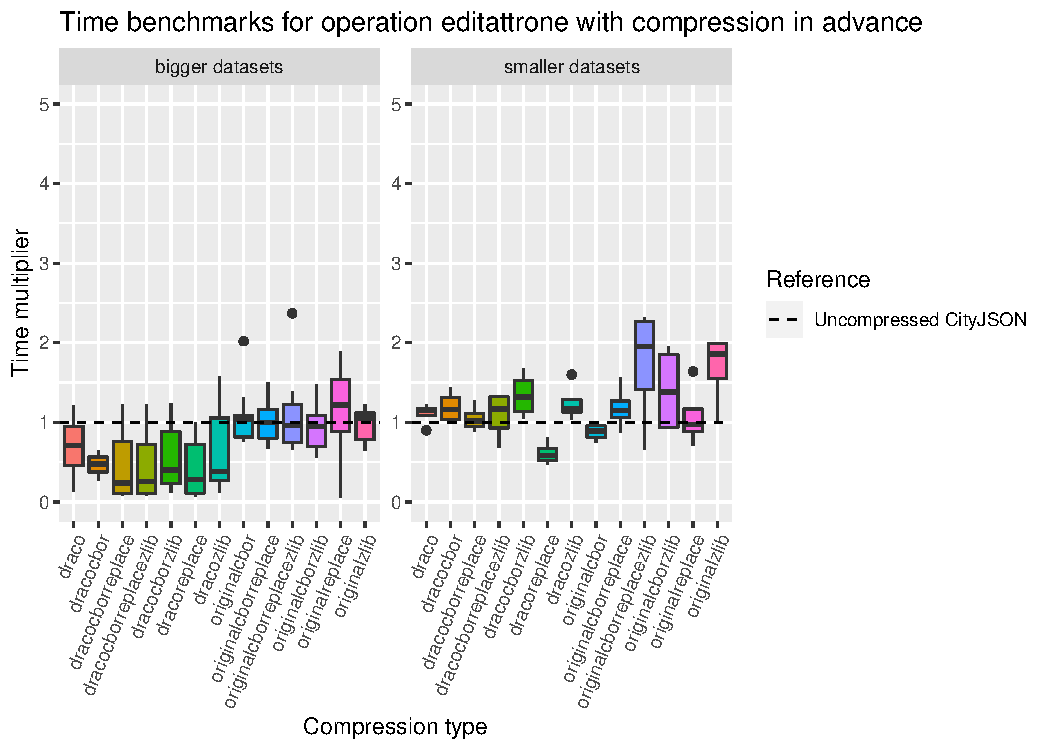
\includegraphics[scale=0.92]{figs/benchmark/individual/editattrone.pdf}
    \caption{Boxplots of time performance of (in advance) compressed datasets on editing attributes of one feature compared to uncompressed CityJSON.}
    \label{fig:sdvis}
\end{figure}

For this use case the compression time becomes relevant, as opposed to the other use cases with compression in advance.
Despite that, the results seem unexpectedly good.
When using Draco compression in combination with large datasets, the performance is rather well both compared to the baseline and to compression types without Draco.
That is because the Draco geometries are not touched as they are not edited, so they also do not need to be compressed again and they make for small file sizes, benefitting the transmission time.
The addition of other compression techniques is beneficial as well since using Draco only does not compare very well to the other Draco compression types.
When not using Draco original-cbor, original-cbor-zlib, and original-zlib do well.

With the small datasets most compression types are not suitable.
Draco-replace does work well which could be explained by the different way in which attributes can be edited with the replace method and the advantage of Draco as mentioned in the paragraph above, but other compression types using this method do not do particularly well. 
Original-cbor is also slightly better than the baseline.

Compression in advance can improve the attribute editing time of CityJSON datasets on one city object to 10\% or 58\% (when respectively using large datasets and small datasets) of the time that it takes to perform the same operation with uncompressed CityJSON.


  \begin{table}[!h]
    \begin{minipage}{.5\linewidth}
      \caption{
Median performance with editattrone on large datasets, compression in advance}
\centering

\begin{tabular}{|l|r|}
\hline
Compression type & median\\
\hline
dracoreplace & 0.100\\
\hline
dracocborreplace & 0.135\\
\hline
dracocborreplacezlib & 0.140\\
\hline
dracocborzlib & 0.335\\
\hline
dracozlib & 0.360\\
\hline
dracocbor & 0.475\\
\hline
originalcborzlib & 0.600\\
\hline
draco & 0.655\\
\hline
originalzlib & 0.730\\
\hline
originalcbor & 0.810\\
\hline
originalcborreplace & 1.015\\
\hline
originalcborreplacezlib & 1.135\\
\hline
originalreplace & 1.330\\
\hline
\end{tabular}
\end{minipage}%
    \begin{minipage}{.5\linewidth}
      \centering
        \caption{
Median performance with editattrone on small datasets, compression in advance}

\begin{tabular}{|l|r|}
\hline
Compression type & median\\
\hline
dracoreplace & 0.580\\
\hline
originalcbor & 0.890\\
\hline
originalreplace & 0.975\\
\hline
dracocborreplace & 1.015\\
\hline
originalcborreplace & 1.150\\
\hline
draco & 1.155\\
\hline
dracocbor & 1.160\\
\hline
dracocborreplacezlib & 1.165\\
\hline
dracozlib & 1.170\\
\hline
dracocborzlib & 1.320\\
\hline
originalcborzlib & 1.380\\
\hline
originalzlib & 1.860\\
\hline
originalcborreplacezlib & 1.955\\
\hline
\end{tabular}
\end{minipage} 
\end{table}



\subsubsection{Compression on the fly}

\begin{figure}[h!]
    %\hspace*{-2.3cm}  
    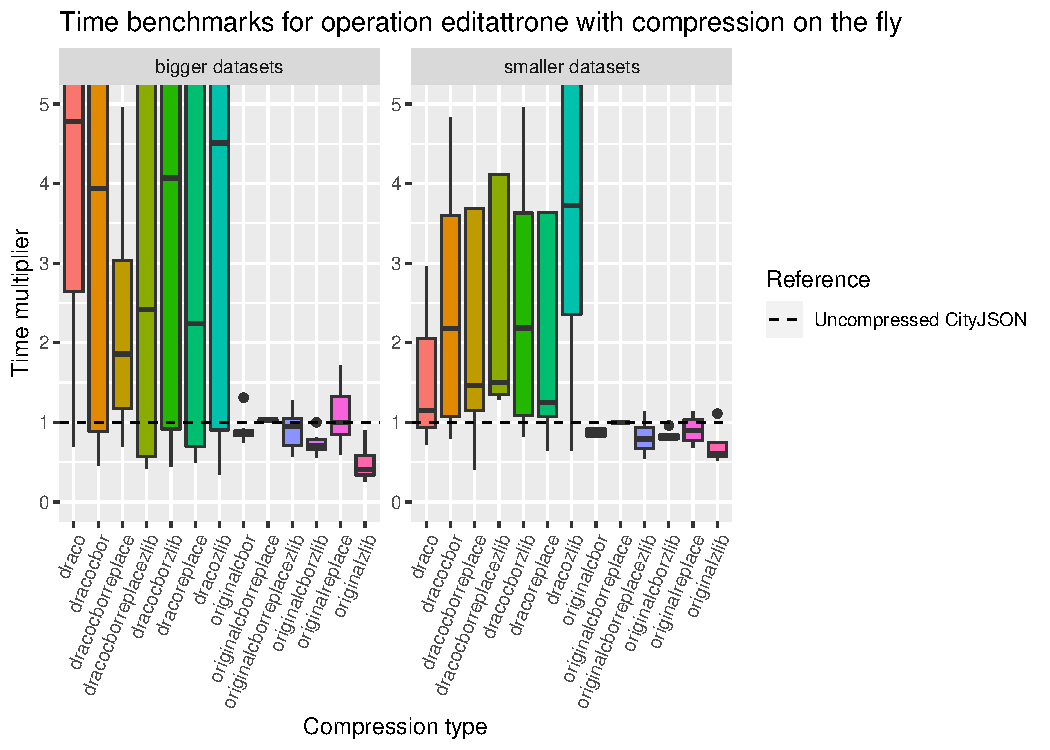
\includegraphics[scale=0.92]{figs/benchmark/individualotf/editattrone.pdf}
    \caption{Boxplots of time performance of (on the fly) compressed datasets on editing attributes of one feature compared to uncompressed CityJSON.}
    \label{figotf:sdvis}
\end{figure}

The data is edited before being compressed with this use case.
Draco is again not suitable to use when compressing data on the fly with neither large nor small datasets.
As for the other compression types, original-zlib and original-cbor-zlib are beneficial for performance with the larger ones, but with the smaller ones only original-cbor and original-cbor-zlib have a (slight) advantage in every case.
The box plots of the other types stretch above the baseline.

On the fly compression can improve the attribute editing time of CityJSON datasets on one city object to 33\% or 60\% (when respectively using large datasets and small datasets) of the time that it takes to perform the same operation with uncompressed CityJSON.



\begin{table}[!h]
    \begin{minipage}{.5\linewidth}
      \caption{
Median performance with editattrone on large datasets, compression on the fly}
\centering

\begin{tabular}{|l|r|}
\hline
Compression type & median\\
\hline
originalzlib & 0.330\\
\hline
dracocborreplacezlib & 0.420\\
\hline
originalcborzlib & 0.570\\
\hline
dracoreplace & 0.760\\
\hline
originalcbor & 0.870\\
\hline
originalcborreplacezlib & 0.960\\
\hline
originalreplace & 1.075\\
\hline
dracocbor & 4.600\\
\hline
dracozlib & 4.990\\
\hline
draco & 5.480\\
\hline
dracocborzlib & 5.610\\
\hline
\end{tabular}
\end{minipage}%
    \begin{minipage}{.5\linewidth}
      \centering
        \caption{
Median performance with editattrone on small datasets, compression on the fly}

\begin{tabular}{|l|r|}
\hline
Compression type & median\\
\hline
originalzlib & 0.605\\
\hline
originalcborreplacezlib & 0.790\\
\hline
originalcborzlib & 0.800\\
\hline
originalcbor & 0.870\\
\hline
originalreplace & 0.900\\
\hline
originalcborreplace & 1.000\\
\hline
draco & 1.150\\
\hline
dracoreplace & 1.250\\
\hline
dracocborreplace & 1.460\\
\hline
dracocborreplacezlib & 1.500\\
\hline
dracocbor & 2.180\\
\hline
dracocborzlib & 2.185\\
\hline
dracozlib & 3.725\\
\hline
\end{tabular}
\end{minipage} 
\end{table}

\newpage


\subsection{Editing attributes all features}

\subsubsection{Compression in advance}

\begin{figure}[h!]
    %\hspace*{-2.3cm}  
    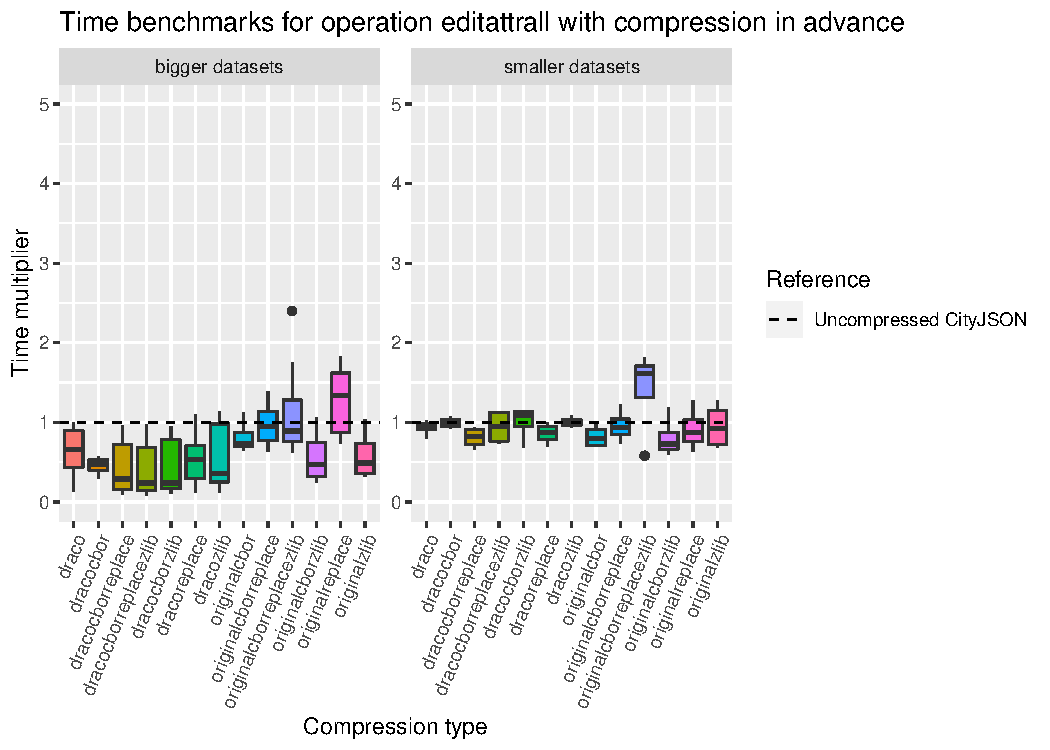
\includegraphics[scale=0.92]{figs/benchmark/individual/editattrall.pdf}
    \caption{Boxplots of time performance of (in advance) compressed datasets on editing attributes of all features compared to uncompressed CityJSON.}
    \label{fig:sdvis}
\end{figure}

When editing the attributes of a large dataset it is not a good idea to use the replace method, regardless of the seemingly more efficient way to edit attributes with it (see Section~\ref{sec:impleditone}).
But apart from that, compression is beneficial for this use case.
Using Draco works well, which would be because it is untouched as only attributes are edited and Draco geometries are small, benefitting the transmission time.
Original-cbor, original-cbor-zlib, and original-zlib also perform well.

With the small datasets most compression types do not always perform well---only draco-cbor-replace has a boxplot that remains under the baseline.
This means that the overhead when compressing the data again does not outweigh the benefits of compression as much as with large datasets.

Compression in advance can improve the attribute editing time of CityJSON datasets on all city objects to 14\% or 72\% (when respectively using large datasets and small datasets) of the time that it takes to perform the same operation with uncompressed CityJSON.


  \begin{table}[!h]
    \begin{minipage}{.5\linewidth}
      \caption{
Median performance with editattrall on large datasets, compression in advance}
\centering

\begin{tabular}{|l|r|}
\hline
Compression type & median\\
\hline
dracocborreplace & 0.140\\
\hline
dracocborreplacezlib & 0.170\\
\hline
dracocborzlib & 0.205\\
\hline
originalcborzlib & 0.300\\
\hline
dracozlib & 0.350\\
\hline
originalzlib & 0.355\\
\hline
dracoreplace & 0.410\\
\hline
dracocbor & 0.475\\
\hline
draco & 0.630\\
\hline
originalcbor & 0.715\\
\hline
originalcborreplace & 1.130\\
\hline
originalreplace & 1.490\\
\hline
originalcborreplacezlib & 1.510\\
\hline
\end{tabular}
\end{minipage}%
    \begin{minipage}{.5\linewidth}
      \centering
        \caption{
Median performance with editattrall on small datasets, compression in advance}

\begin{tabular}{|l|r|}
\hline
Compression type & median\\
\hline
originalcborzlib & 0.725\\
\hline
originalcbor & 0.795\\
\hline
dracocborreplace & 0.820\\
\hline
dracoreplace & 0.870\\
\hline
originalreplace & 0.875\\
\hline
originalzlib & 0.925\\
\hline
originalcborreplace & 0.935\\
\hline
dracocborreplacezlib & 0.945\\
\hline
draco & 0.965\\
\hline
dracocbor & 0.995\\
\hline
dracozlib & 0.995\\
\hline
dracocborzlib & 1.090\\
\hline
originalcborreplacezlib & 1.615\\
\hline
\end{tabular}
\end{minipage} 
\end{table}

\clearpage

\subsubsection{Compression on the fly}

\begin{figure}[h!]
    %\hspace*{-2.3cm}  
    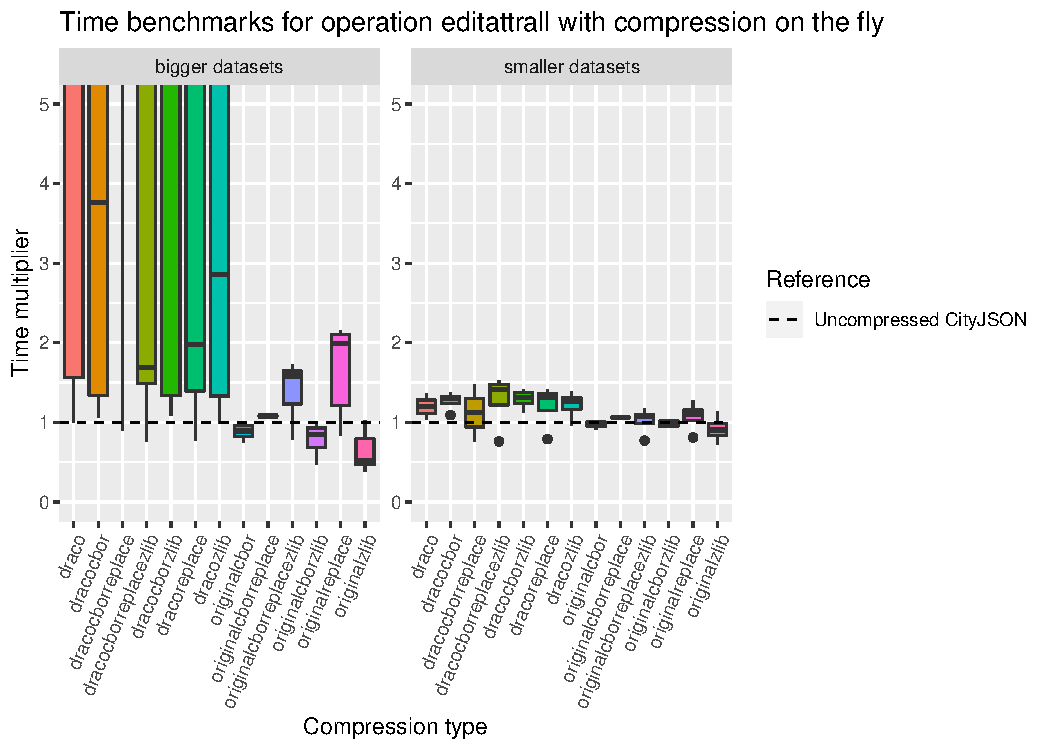
\includegraphics[scale=0.92]{figs/benchmark/individualotf/editattrall.pdf}
    \caption{Boxplots of time performance of (on the fly) compressed datasets on editing attributes of all features compared to uncompressed CityJSON.}
    \label{figotf:sdvis}
\end{figure}


As is always the case with compression on the fly, the use of Draco compression is detrimental for performance.
With the large datasets original-cbor, original-cbor-zlib, and original-zlib yield a proper performance gain, which would be the result of a good balance between file size and (de)compression time.
As for the small datasets, the differences between the compression types are smaller and there is no clear best one to use as the better performing ones are around the baseline.
Thus in that case you might be better off not using compression at all.


On the fly compression can improve the attribute editing time of CityJSON datasets on all city objects to 47\% or 90\% (when respectively using large datasets and small datasets) of the time that it takes to perform the same operation with uncompressed CityJSON.



  \begin{table}[!h]
    \begin{minipage}{.5\linewidth}
      \caption{
Median performance with editattrall on large datasets, compression on the fly}
\centering

\begin{tabular}{|l|r|}
\hline
Compression type & median\\
\hline
originalzlib & 0.475\\
\hline
originalcborzlib & 0.680\\
\hline
originalcbor & 0.825\\
\hline
originalcborreplacezlib & 1.660\\
\hline
originalreplace & 2.105\\
\hline
dracoreplace & 15.180\\
\hline
dracozlib & 16.910\\
\hline
dracocborreplacezlib & 16.950\\
\hline
draco & 18.210\\
\hline
dracocborreplace & 27.220\\
\hline
dracocborzlib & 28.735\\
\hline
dracocbor & 32.745\\
\hline
\end{tabular}
\end{minipage}%
    \begin{minipage}{.5\linewidth}
      \centering
        \caption{
Median performance with editattrall on small datasets, compression on the fly}

\begin{tabular}{|l|r|}
\hline
Compression type & median\\
\hline
originalzlib & 0.905\\
\hline
originalcbor & 0.980\\
\hline
originalcborzlib & 0.980\\
\hline
originalcborreplace & 1.060\\
\hline
originalcborreplacezlib & 1.070\\
\hline
originalreplace & 1.105\\
\hline
dracocborreplace & 1.120\\
\hline
draco & 1.200\\
\hline
dracozlib & 1.260\\
\hline
dracocbor & 1.300\\
\hline
dracoreplace & 1.310\\
\hline
dracocborzlib & 1.315\\
\hline
dracocborreplacezlib & 1.415\\
\hline
\end{tabular}
\end{minipage} 
\end{table}

\clearpage

\section{Editing (geometry)}
\label{bmeditinggeom}

\subsection{Editing geometry one feature}
\label{sec:bmeditone}

\subsubsection{Compression in advance}


\begin{figure}[h!]
    %\hspace*{-2.3cm}  
    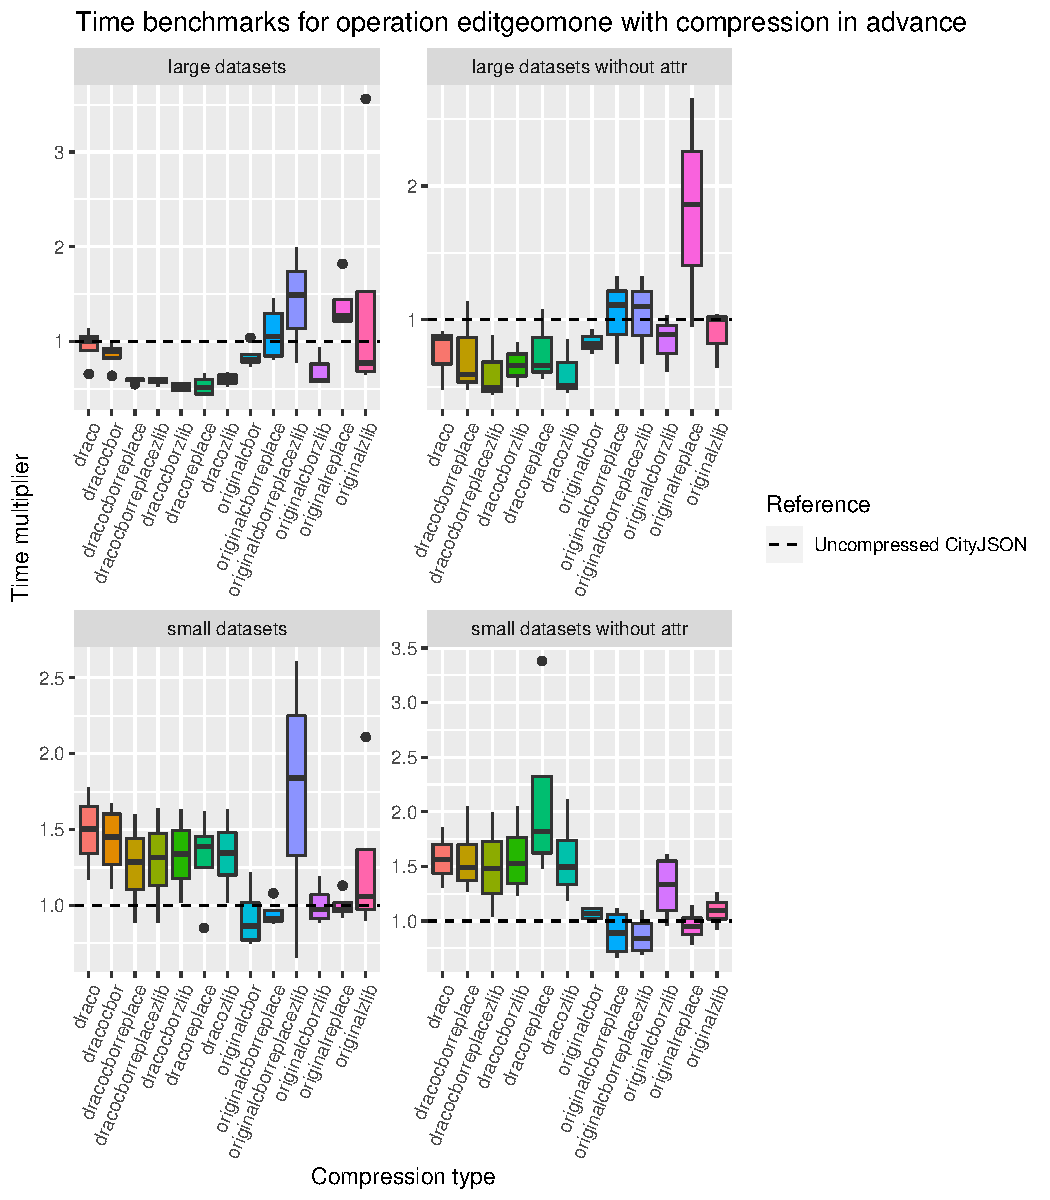
\includegraphics[scale=0.92]{figs/benchmark/individual/editgeomone.pdf}
    \caption{Boxplots of time performance of (in advance) compressed datasets on editing geometry of one feature compared to uncompressed CityJSON.}
    \label{fig:sdvis}
\end{figure}

Draco is suitable for this use case when editing large datasets.
This is despite Draco methods having high compression times as shown in Section~\ref{sec:encodingperformance}.
But the results in that Section were created by compressing CityJSON geometries into Draco geometries with OBJ conversion as intermediate step (see Section~\ref{sec:dracocompressiontypes}).
In this case however the Draco geometries are edited directly as they are decoded in the client.
It can then be compressed again without additional steps.
The use of additional compression techniques is beneficial as well.
If not using Draco, original-cbor and original-cbor-zlib are good choices.
This is the same for datasets that do not contain attributes.

With the small datasets none of the compression types perform particularly well.
Draco is now not beneficial which would be due to the overhead of Draco compression that is more significant with small data.
Original-cbor has the lowest median with attributes, but is above the baseline with datasets that do not have attributes.
In that case there is less data for \ac{cbor} to compress which could be the explaining factor.

Compression in advance can improve the geometry editing time of CityJSON datasets on one city object to 51\%, 49\%, 86\%, or 84\% (when respectively using large datasets, large datasets without attributes, small datasets, and small datasets without attributes) of the time that it takes to perform the same operation with uncompressed CityJSON.



  \begin{table}[!h]
    \begin{minipage}{.5\linewidth}
      \caption{
Median performance with editgeomone on large datasets, compression in advance}
\centering

\begin{tabular}{|l|r|}
\hline
Compression type & median\\
\hline
dracoreplace & 0.515\\
\hline
dracocborzlib & 0.520\\
\hline
originalcborzlib & 0.590\\
\hline
dracocborreplacezlib & 0.595\\
\hline
dracocborreplace & 0.600\\
\hline
dracozlib & 0.605\\
\hline
originalzlib & 0.775\\
\hline
originalcbor & 0.805\\
\hline
dracocbor & 0.895\\
\hline
draco & 1.005\\
\hline
originalcborreplace & 1.055\\
\hline
originalreplace & 1.270\\
\hline
originalcborreplacezlib & 1.490\\
\hline
\end{tabular}
\end{minipage}%
    \begin{minipage}{.5\linewidth}
      \centering
        \caption{
Median performance with editgeomone on large datasets without attributes, compression in advance}

\begin{tabular}{|l|r|}
\hline
Compression type & median\\
\hline
dracocborreplacezlib & 0.49\\
\hline
dracozlib & 0.51\\
\hline
dracocborreplace & 0.59\\
\hline
dracocborzlib & 0.66\\
\hline
dracoreplace & 0.66\\
\hline
originalcbor & 0.82\\
\hline
draco & 0.86\\
\hline
originalcborzlib & 0.89\\
\hline
originalzlib & 1.00\\
\hline
originalcborreplacezlib & 1.10\\
\hline
originalcborreplace & 1.11\\
\hline
originalreplace & 1.86\\
\hline
\end{tabular}
\end{minipage} 
\end{table}
\begin{table}[!h]
    \begin{minipage}{.5\linewidth}
      \caption{
Median performance with editgeomone on small datasets, compression in advance}
\centering

\begin{tabular}{|l|r|}
\hline
Compression type & median\\
\hline
originalcbor & 0.865\\
\hline
originalcborreplace & 0.915\\
\hline
originalreplace & 0.975\\
\hline
originalcborzlib & 0.975\\
\hline
originalzlib & 1.060\\
\hline
dracocborreplace & 1.285\\
\hline
dracocborreplacezlib & 1.315\\
\hline
dracocborzlib & 1.340\\
\hline
dracozlib & 1.345\\
\hline
dracoreplace & 1.390\\
\hline
dracocbor & 1.450\\
\hline
draco & 1.505\\
\hline
originalcborreplacezlib & 1.840\\
\hline
\end{tabular}
\end{minipage}%
    \begin{minipage}{.5\linewidth}
      \centering
        \caption{
Median performance with editgeomone on small datasets without attributes, compression in advance}

\begin{tabular}{|l|r|}
\hline
Compression type & median\\
\hline
originalcborreplacezlib & 0.840\\
\hline
originalcborreplace & 0.890\\
\hline
originalreplace & 0.950\\
\hline
originalcbor & 1.070\\
\hline
originalzlib & 1.095\\
\hline
originalcborzlib & 1.335\\
\hline
dracocborreplacezlib & 1.480\\
\hline
dracocborreplace & 1.490\\
\hline
dracozlib & 1.495\\
\hline
dracocborzlib & 1.525\\
\hline
draco & 1.565\\
\hline
dracoreplace & 1.820\\
\hline
\end{tabular}
\end{minipage} 
\end{table}

\clearpage

\subsubsection{Compression on the fly}

\begin{figure}[h!]
    %\hspace*{-2.3cm}  
    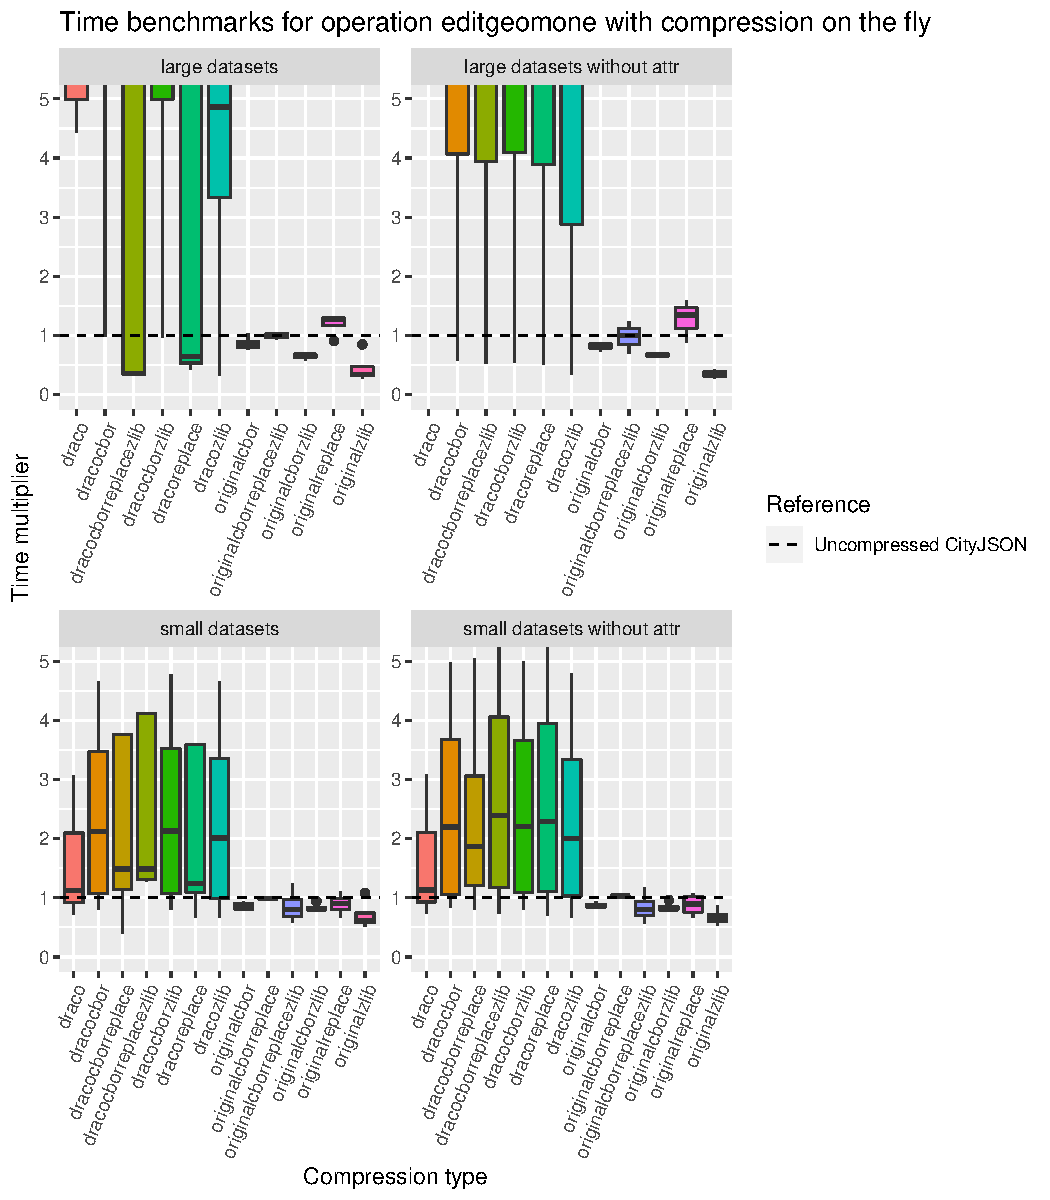
\includegraphics[scale=0.92]{figs/benchmark/individualotf/editgeomone.pdf}
    \caption{Boxplots of time performance of (on the fly) compressed datasets on editing geometry of one feature compared to uncompressed CityJSON.}
    \label{figotf:sdvis}
\end{figure}

Ignoring the compression types using Draco, it can be beneficial to use compression on the fly for this use case.
With large datasets, original-cbor, original-zlib, and original-cbor-zlib do well.
They are also fine to use with small datasets, but here the compression types have similar performances.
There are no other notable observations to be made.

On the fly compression can improve the geometry editing time of CityJSON datasets on one city object to 34\%, 36\%, 61\%, or 64\% (when respectively using large datasets, large datasets without attributes, small datasets, and small datasets without attributes) of the time that it takes to perform the same operation with uncompressed CityJSON.



  \begin{table}[!h]
    \begin{minipage}{.5\linewidth}
      \caption{
Median performance with editgeomone on large datasets, compression on the fly}
\centering

\begin{tabular}{|l|r|}
\hline
Compression type & median\\
\hline
originalzlib & 0.345\\
\hline
dracocborreplacezlib & 0.360\\
\hline
dracoreplace & 0.650\\
\hline
originalcborzlib & 0.680\\
\hline
originalcbor & 0.830\\
\hline
originalcborreplacezlib & 1.000\\
\hline
originalreplace & 1.270\\
\hline
dracozlib & 4.860\\
\hline
draco & 5.540\\
\hline
dracocborzlib & 9.020\\
\hline
dracocbor & 11.700\\
\hline
\end{tabular}
\end{minipage}%
    \begin{minipage}{.5\linewidth}
      \centering
        \caption{
Median performance with editgeomone on large datasets without attributes, compression on the fly}

\begin{tabular}{|l|r|}
\hline
Compression type & median\\
\hline
originalzlib & 0.36\\
\hline
originalcborzlib & 0.66\\
\hline
originalcbor & 0.85\\
\hline
originalcborreplacezlib & 1.00\\
\hline
originalreplace & 1.35\\
\hline
dracozlib & 5.42\\
\hline
draco & 6.60\\
\hline
dracoreplace & 7.26\\
\hline
dracocborreplacezlib & 7.37\\
\hline
dracocbor & 7.56\\
\hline
dracocborzlib & 7.63\\
\hline
\end{tabular}
\end{minipage} 
\end{table}
\begin{table}[!h]
    \begin{minipage}{.5\linewidth}
      \caption{
Median performance with editgeomone on small datasets, compression on the fly}
\centering

\begin{tabular}{|l|r|}
\hline
Compression type & median\\
\hline
originalzlib & 0.615\\
\hline
originalcborreplacezlib & 0.800\\
\hline
originalcborzlib & 0.805\\
\hline
originalcbor & 0.855\\
\hline
originalreplace & 0.900\\
\hline
originalcborreplace & 0.990\\
\hline
draco & 1.120\\
\hline
dracoreplace & 1.240\\
\hline
dracocborreplacezlib & 1.485\\
\hline
dracocborreplace & 1.490\\
\hline
dracozlib & 2.010\\
\hline
dracocbor & 2.120\\
\hline
dracocborzlib & 2.130\\
\hline
\end{tabular}
\end{minipage}%
    \begin{minipage}{.5\linewidth}
      \centering
        \caption{
Median performance with editgeomone on small datasets without attributes, compression on the fly}

\begin{tabular}{|l|r|}
\hline
Compression type & median\\
\hline
originalzlib & 0.640\\
\hline
originalcborreplacezlib & 0.805\\
\hline
originalcborzlib & 0.815\\
\hline
originalcbor & 0.865\\
\hline
originalreplace & 0.895\\
\hline
originalcborreplace & 1.030\\
\hline
draco & 1.130\\
\hline
dracocborreplace & 1.870\\
\hline
dracozlib & 2.000\\
\hline
dracocbor & 2.195\\
\hline
dracocborzlib & 2.205\\
\hline
dracoreplace & 2.290\\
\hline
dracocborreplacezlib & 2.390\\
\hline
\end{tabular}
\end{minipage} 
\end{table}

\newpage

\subsection{Editing geometry all features}


\subsubsection{Compression in advance}

\begin{figure}[h!]
    %\hspace*{-2.3cm}  
    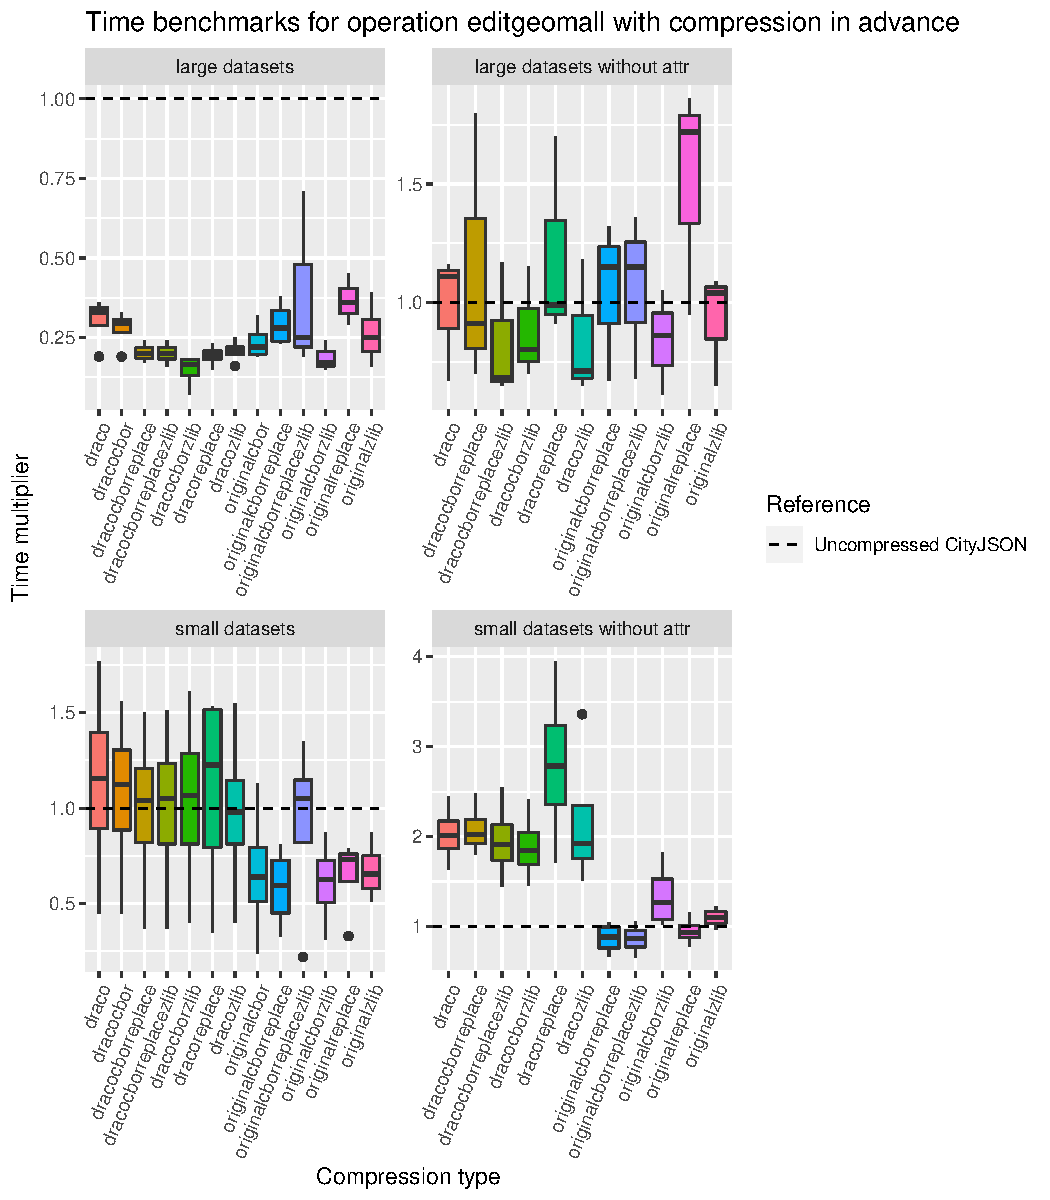
\includegraphics[scale=0.92]{figs/benchmark/individual/editgeomall.pdf}
    \caption{Boxplots of time performance of (in advance) compressed datasets on editing geometry of all features compared to uncompressed CityJSON.}
    \label{fig:sdvis}
\end{figure}

With the large datasets that include attributes all compression types perform well.
This is not seen when only editing the geometry of one city object, when performance was only good with Draco.
It is surprising because now all city objects have to be traversed for compression types without Draco, but with Draco all vertices already had to be iterated over, even when just wanting to edit one feature (see Section~\ref{sec:impleditgeomone}).
The results are also quite different for large datasets without attributes, and generally worse---none of the compression types is good to use with every of these datasets as the boxplots indicate.
This is surprising as well since there is less data to compress again after the editing in that case.

As for the small datasets, Draco compresses negatively influences the performance, presumably because of the overhead.
Other compression types generally work well, except for draco-cbor-replace-zlib when attributes are included and original-cbor-zlib when they are not.
The latter one tends to perform well in other use cases so it could be an anomaly.
The former type includes the replace method that does not do well so far, but other compression types that use it do not do as bad.
This can indicate that it is not worth it to compress the array of attributes with zlib (see Section~\ref{sec:implreplace}).

Compression in advance can improve the geometry editing time of CityJSON datasets on all city objects to 16\%, 68\%, 59\%, or 86\% (when respectively using large datasets, large datasets without attributes, small datasets, and small datasets without attributes) of the time that it takes to perform the same operation with uncompressed CityJSON.


  \begin{table}[!h]
    \begin{minipage}{.5\linewidth}
      \caption{
Median performance with editgeomall on large datasets, compression in advance}
\centering

\begin{tabular}{|l|r|}
\hline
Compression type & median\\
\hline
dracocborzlib & 0.165\\
\hline
originalcborzlib & 0.170\\
\hline
dracoreplace & 0.195\\
\hline
dracocborreplace & 0.200\\
\hline
dracocborreplacezlib & 0.200\\
\hline
dracozlib & 0.210\\
\hline
originalcbor & 0.220\\
\hline
originalcborreplacezlib & 0.250\\
\hline
originalzlib & 0.250\\
\hline
originalcborreplace & 0.280\\
\hline
dracocbor & 0.295\\
\hline
draco & 0.330\\
\hline
originalreplace & 0.360\\
\hline
\end{tabular}
\end{minipage}%
    \begin{minipage}{.5\linewidth}
      \centering
        \caption{
Median performance with editgeomall on large datasets without attributes, compression in advance}

\begin{tabular}{|l|r|}
\hline
Compression type & median\\
\hline
dracocborreplacezlib & 0.68\\
\hline
dracozlib & 0.71\\
\hline
dracocborzlib & 0.80\\
\hline
originalcborzlib & 0.86\\
\hline
dracocborreplace & 0.91\\
\hline
dracoreplace & 0.99\\
\hline
originalzlib & 1.04\\
\hline
draco & 1.11\\
\hline
originalcborreplace & 1.15\\
\hline
originalcborreplacezlib & 1.15\\
\hline
originalreplace & 1.72\\
\hline
\end{tabular}
\end{minipage} 
\end{table}
\begin{table}[!h]
    \begin{minipage}{.5\linewidth}
      \caption{
Median performance with editgeomall on small datasets, compression in advance}
\centering

\begin{tabular}{|l|r|}
\hline
Compression type & median\\
\hline
originalcborreplace & 0.595\\
\hline
originalcborzlib & 0.625\\
\hline
originalcbor & 0.640\\
\hline
originalzlib & 0.655\\
\hline
originalreplace & 0.730\\
\hline
dracozlib & 0.980\\
\hline
dracocborreplace & 1.040\\
\hline
dracocborreplacezlib & 1.050\\
\hline
originalcborreplacezlib & 1.050\\
\hline
dracocborzlib & 1.065\\
\hline
dracocbor & 1.125\\
\hline
draco & 1.155\\
\hline
dracoreplace & 1.225\\
\hline
\end{tabular}
\end{minipage}%
    \begin{minipage}{.5\linewidth}
      \centering
        \caption{
Median performance with editgeomall on small datasets without attributes, compression in advance}

\begin{tabular}{|l|r|}
\hline
Compression type & median\\
\hline
originalcborreplacezlib & 0.865\\
\hline
originalcborreplace & 0.885\\
\hline
originalreplace & 0.935\\
\hline
originalzlib & 1.100\\
\hline
originalcborzlib & 1.265\\
\hline
dracocborzlib & 1.845\\
\hline
dracocborreplacezlib & 1.910\\
\hline
dracozlib & 1.925\\
\hline
draco & 2.010\\
\hline
dracocborreplace & 2.025\\
\hline
dracoreplace & 2.785\\
\hline
\end{tabular}
\end{minipage} 
\end{table}

\clearpage

\subsubsection{Compression on the fly}

\begin{figure}[h!]
    %\hspace*{-2.3cm}  
    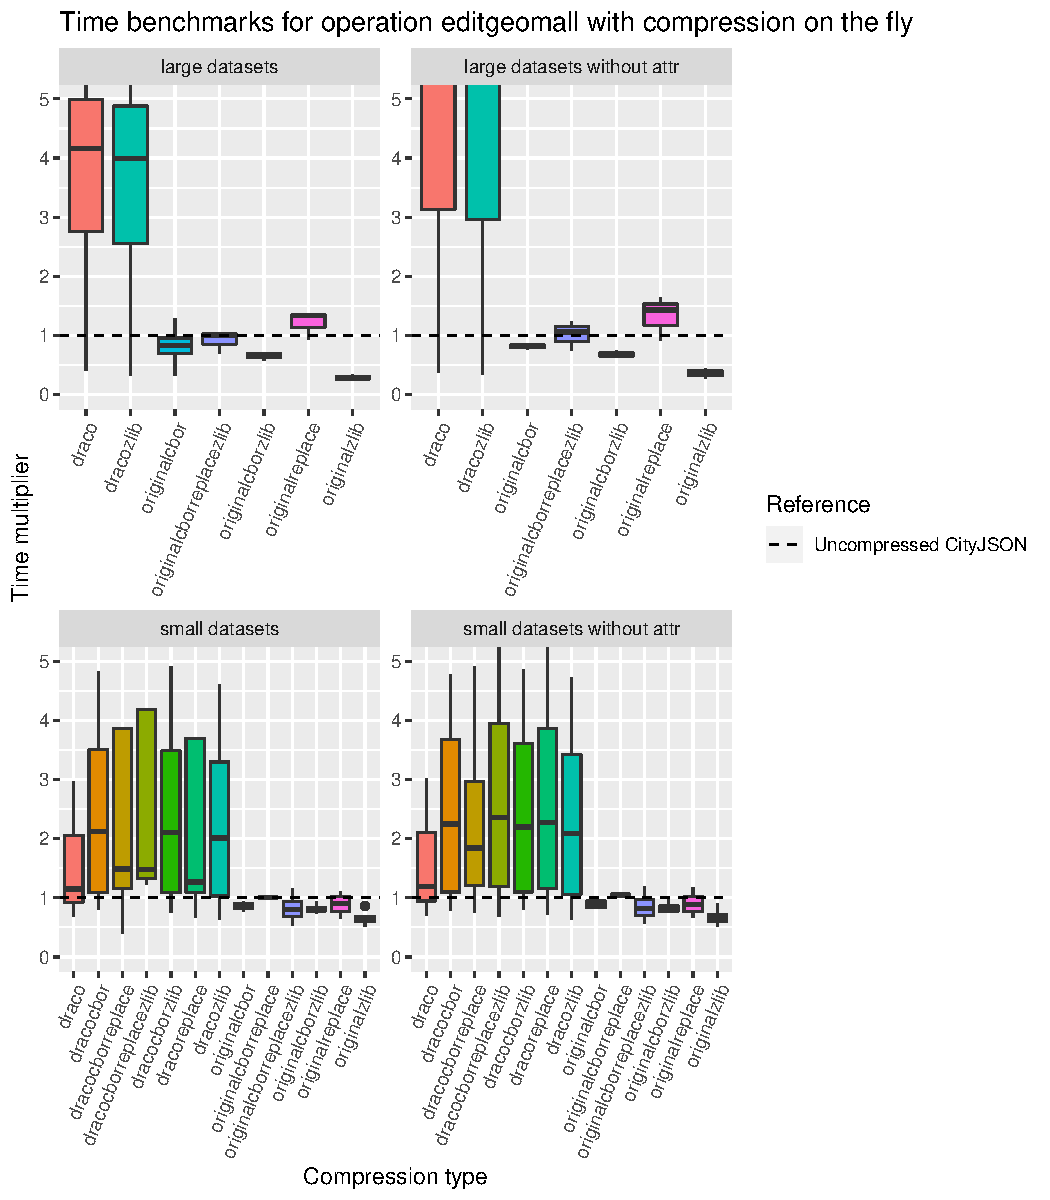
\includegraphics[scale=0.92]{figs/benchmark/individualotf/editgeomall.pdf}
    \caption{Boxplots of time performance of (on the fly) compressed datasets on editing geometry of all features compared to uncompressed CityJSON.}
    \label{figotf:sdvis}
\end{figure}

There was an error with multiple compression types in combination with this use case and large datasets, which is why they are missing from the charts.
It is not very important, since it was mostly a problem with Draco which has already proven to perform badly with on the fly compression.

What happens in this use case is that basically full datasets are compressed after all being edited with the same algorithm.
The results are thus not so interesting and should come close to the theoretical perormance gain.
With the large datasets original-zlib and original-cbor-zlib do well, and original-cbor as well when attributes are not included.
As for the small datasets, these three do well with both small dataset types.
They are relatively uncomplicated compression types and their good performance can be explained by the balance between file size and processing time, despite compression time being included.

On the fly compression can improve the geometry editing time of CityJSON datasets on all city objects to 28\%, 37\%, 62\%, or 64\% (when respectively using large datasets, large datasets without attributes, small datasets, and small datasets without attributes) of the time that it takes to perform the same operation with uncompressed CityJSON.


\begin{table}[!h]
    \begin{minipage}{.5\linewidth}
      \caption{
Median performance with editgeomall on large datasets, compression on the fly}
\centering

\begin{tabular}{|l|r|}
\hline
Compression type & median\\
\hline
originalzlib & 0.280\\
\hline
originalcborzlib & 0.680\\
\hline
originalcbor & 0.835\\
\hline
originalcborreplacezlib & 1.010\\
\hline
originalreplace & 1.340\\
\hline
dracozlib & 3.995\\
\hline
draco & 4.165\\
\hline
\end{tabular}
\end{minipage}%
    \begin{minipage}{.5\linewidth}
      \centering
        \caption{
Median performance with editgeomall on large datasets without attributes, compression on the fly}

\begin{tabular}{|l|r|}
\hline
Compression type & median\\
\hline
originalzlib & 0.37\\
\hline
originalcborzlib & 0.66\\
\hline
originalcbor & 0.83\\
\hline
originalcborreplacezlib & 1.06\\
\hline
originalreplace & 1.43\\
\hline
dracozlib & 5.58\\
\hline
draco & 5.89\\
\hline
\end{tabular}
\end{minipage} 
\end{table}
\begin{table}[!h]
    \begin{minipage}{.5\linewidth}
      \caption{
Median performance with editgeomall on small datasets, compression on the fly}
\centering

\begin{tabular}{|l|r|}
\hline
Compression type & median\\
\hline
originalzlib & 0.625\\
\hline
originalcborreplacezlib & 0.800\\
\hline
originalcborzlib & 0.800\\
\hline
originalcbor & 0.870\\
\hline
originalreplace & 0.905\\
\hline
originalcborreplace & 1.010\\
\hline
draco & 1.150\\
\hline
dracoreplace & 1.265\\
\hline
dracocborreplacezlib & 1.480\\
\hline
dracocborreplace & 1.485\\
\hline
dracozlib & 2.010\\
\hline
dracocborzlib & 2.105\\
\hline
dracocbor & 2.125\\
\hline
\end{tabular}
\end{minipage}%
    \begin{minipage}{.5\linewidth}
      \centering
        \caption{
Median performance with editgeomall on small datasets without attributes, compression on the fly}

\begin{tabular}{|l|r|}
\hline
Compression type & median\\
\hline
originalzlib & 0.640\\
\hline
originalcborzlib & 0.800\\
\hline
originalcborreplacezlib & 0.820\\
\hline
originalreplace & 0.885\\
\hline
originalcbor & 0.890\\
\hline
originalcborreplace & 1.050\\
\hline
draco & 1.190\\
\hline
dracocborreplace & 1.840\\
\hline
dracozlib & 2.090\\
\hline
dracocborzlib & 2.195\\
\hline
dracocbor & 2.250\\
\hline
dracoreplace & 2.275\\
\hline
dracocborreplacezlib & 2.355\\
\hline
\end{tabular}
\end{minipage} 
\end{table}



\newpage
\section{Conclusion and recommendations}
\label{bmconclusion}

\begin{figure}[h!]
    %\hspace*{-2.3cm}  
    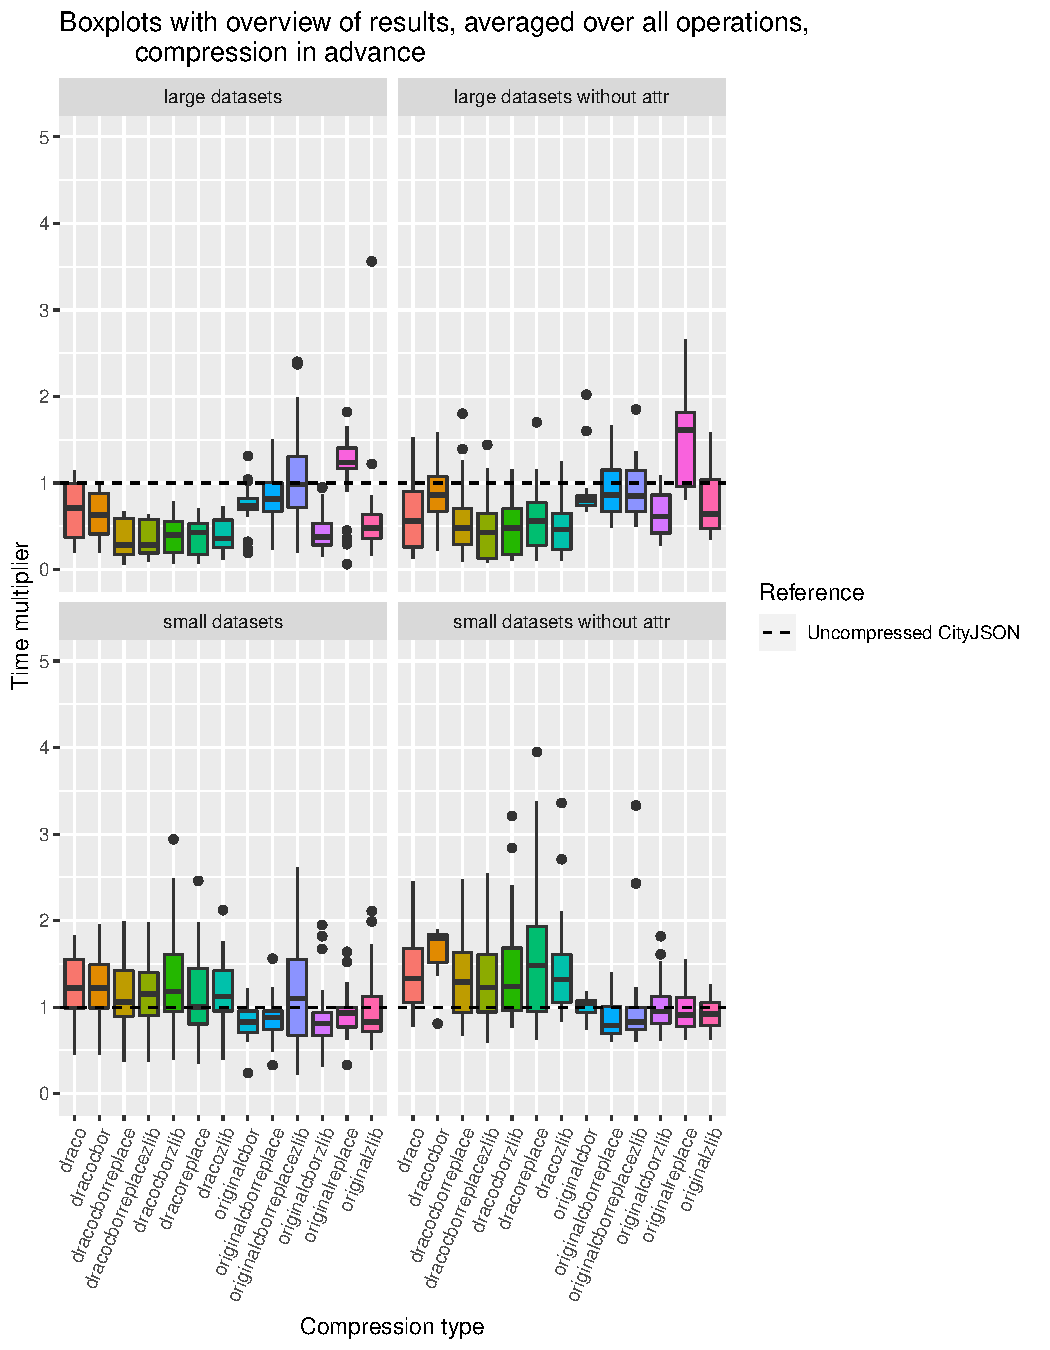
\includegraphics[scale=0.92]{figs/benchmark/overview/fulloverviewia.pdf}
    \caption{Overview of the performance of all compression types by dataset type. The results are averaged over every operation.}
    \label{fig:performanceoverview}
\end{figure}

\begin{figure}[h!]
    %\hspace*{-2.3cm}  
    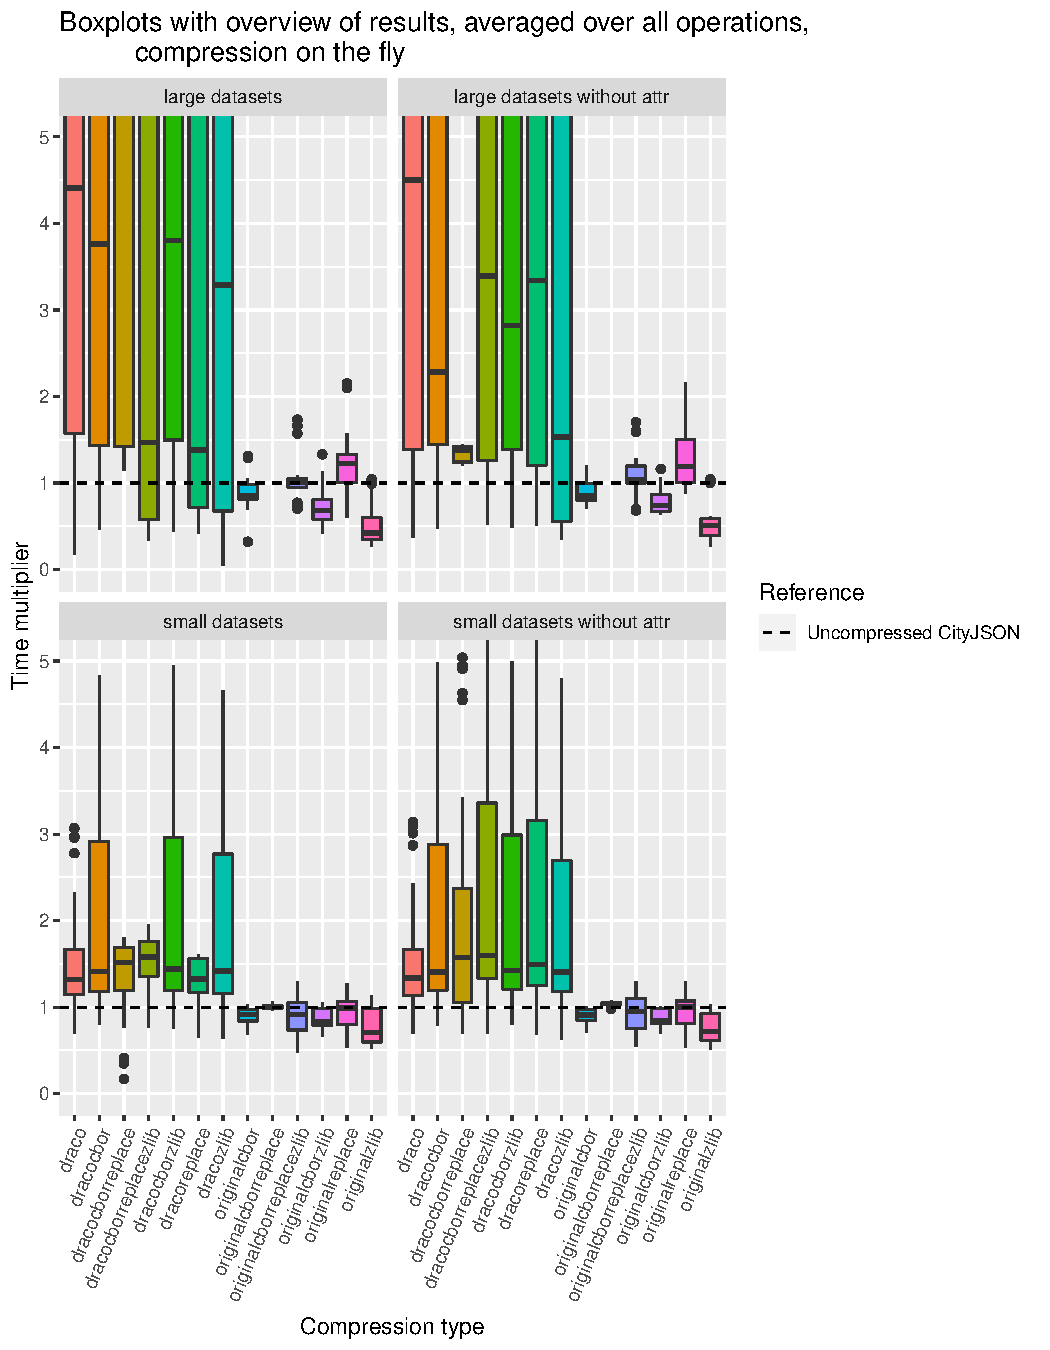
\includegraphics[scale=0.92]{figs/benchmark/overview/fulloverviewotf.pdf}
    \caption{Overview of the performance of all compression types by dataset type. The results are averaged over every operation.}
    \label{fig:performanceoverviewotf}
\end{figure}

\clearpage


On Figures~\ref{fig:performanceoverview} and ~\ref{fig:performanceoverviewotf}, the difference between operations is removed here such that appropriate compression types for general purpose can be found.
It is possible to pick a best one based on specific cases---for a dataset type and operation combination that is known beforehand.
You can see in the presented charts which compression type you should then choose for the best performance.
But sometimes a software developer would want to write flexible software that works well with a larger variety of use cases, rather than creating it for visualisation or editing only.
Additionally, implementating multiple compression types for CityJSON will make it more complex as a file type, because all software that uses it would need to be able to handle all the compressed versions.
For these reasons these overviews are given, such that compression types that perform well in most cases can be identified.




\subsubsection{Compression in advance}

With the large datasets with attributes, the inclusion of Draco geometry is clearly beneficial for performance.
This is especially so when it is combined with additional compression techniques.
Draco-cbor-replace, draco-cbor-replace-zlib, draco-cbor-zlib, draco-replace, and draco-zlib all perform under the baseline with every operation.
This is also true for original-cbor-zlib. Original-cbor and originall-zlib are also good most of the time.
This is similar for the large datasets without attributes.
But generally, the results are less good and all of them do reach above the baseline for some specific operations.
This indicates that the compression of attributes is actually of importance, since if they are not there, compression has less benefits as compared to attributes being included in the datasets.

Regarding the small datasets it is not as beneficial to compress datasets, both with and without attributes.
In Chapter~\ref{chap:introduction} I had already stated that the main goal of the thesis was to improve the performance with large files, and it is what I had expected to be improved the most.
But original-cbor, original-cbor-replace, original-cbor-zlib, original-replace, and original-zlib still have median outcomes under the baseline with the small datasets that include attributes.
This is similar for the ones without attributes, except that original-cbor-replace-zlib proved to also be beneficial overall, and original-cbor is a bit above the baseline.
Draco compression is most of the time not useful with these dataset types since it adds overhead that is not compensated for by the lowered transmission time.

%\begin{table}[]
%\begin{tabular}{|l|l|l|l|l|l|l|l|l|}
%\hline
%\multicolumn{3}{c}{Visualise}                       &  \multicolumn{3}{c}{Visualise}          &    \multicolumn{3}{c}{Visualise}  \\ \hline
%Larger          & dracocborreplace & 0.375            &           &           &           &           &           &           \\ \hline
%Larger noattr           & dracocborreplacezlib & 0.39            &           &           &           &           &           &           \\\hline
%Smaller           & originalcborzlib & 0.730            &           &           &           &           &           &           \\\hline
%Smaller noattr           & originalcborreplacezlib & 0.805            &           &           &           &           &           &           \\  \hline
 %          &            &            &           &           &           &           &           &           \\ \hline
  %         &            &            &           &           &           &           &           &           \\ \hline
%\end{tabular}
%\end{table}


\subsubsection{Compression on the fly}

As opposed to compression in advance, the use of Draco is never a good idea when compressing data on the fly.
This is due to the long compression times (see Section~\ref{sec:encodingperformance}) of Draco, which is partially because of the intermediate conversion of CityJSON geometries to OBJ.
As for compression types that retain original geometry, the boxplots also reach above the uncompressed CityJSON baseline when large datasets are processed.
This means that there is none that is beneficial for any operation.
But still, original-cbor, original-zlib, and original-cbor-zlib are useful if you look at the median results.

This also holds true with the small datasets, with the difference being that original-cbor-replace-zlib has a median just below the baseline as well.
But most of the time, compression is still more useful with large datasets.
In general the inclusion of attributes does not make a noticeable difference in the results.

\subsubsection{Discussion}

When interpreting the results it has also to be kept in mind that the baseline for the performance of small datasets is already small.
A time multiplier of 0.5 looks nice, but in the end you are often talking about milliseconds saved.
However, this can add up when a lot of data is processed.
Also, for bigger datasets, the time saved can be seconds to even minutes.

Concludingly, I have deliberately not singled out "best" compression types in the benchmarking conclusion because I think it is not possible based on these graphs, as there are no clear winners.
In the previous Sections the best compression types for specific use cases can be seen, but I think a compression type that is actually implemented needs to do well all-round, because the implementation of multiple ones makes the development of software extra complicated.
Additionally, these results only show performance but not the ease of implementation of the compression types, which is discussed in Chapter~\ref{ch:conclusion}.

Generally, compression gives the greatest benefits when large datasets are used.
The removal of attributes from datasets does not show any noticeable differences in outcome.
While Draco compression does show good results, it does not work well all-round, especially when you consider small files and with on the fly compression.
The replace method often is not beneficial either, and it does require the traversal of all city objects for both compression and decompression, which turns out to not be efficient.
Considering both all-round performance and ease of use, I think that original-cbor, original-zlib, and original-cbor-zlib are the most suitable best compression types.
They improve the general performance as can be seen from their median values in Figure~\ref{fig:performanceoverview}.
At the same time they are easy to implement, as both CBOR and zlib only need one line of code for encoding of decoding (see Section~\ref{sec:gzipcborcombo}).
Additionally they are widely supported and have libraries in many programming languages \citep{CBOR2020, zlib2020}.


%%!TEX root = thesis.tex
\chapter{Other efficient web-use}
\label{chap:r2}

\section{OGC API}

\section{Tiling}

\section{Streaming CityJSON}
%!TEX root = thesis.tex
\chapter{Conclusion}
\label{ch:conclusion}

\section{Performed work and summary of achieved results}

In the end I have tested 16 CityJSON datasets, represented in 14 different ways, on 9 operations in two different ways: with the datasets prepared in advance, and with them being compressed on the fly.
This makes for 4032 benchmarks that have been condensed into 18 boxplot charts in Chapter~\ref{ch:bmresults}, accompanied by additional benchmarks on (de)compression time and file size that help explaining the results.
For every use case, the best-performing compression type has been found.
I have also created two overview graphs for the two server implementations, which indicate what compression types have a good all-round performance compared to original CityJSON.

In some cases, I have achieved results of as good as 9\% of the time that it would to take the same operation with uncompressed CityJSON---when buffering the city objects of all larger datasets (that include attributes), with a file that is compressed beforehand with the draco-cbor-zlib type.
This is however a very specific use case, and there are also cases in which compression is not worth it.
For example, when querying one city object and compressing it on the fly.

The research question of the thesis is as follows:

\textit{To what extent can the implementation of different compression techniques improve CityJSON’s performance on the web, considering file size, visualisation, querying, spatial analysis, and editing performance?}

You could theoretically answer the question by stating the numbers of the best benchmarking results for every use case.
I however think it does not make sense to state specific numbers to answer this question as I believe it does not matter for the actually useful conclusions of this thesis.
The use cases are too specific and it is not a good idea to implement multiple compression types for specific cases only.
It turned out to be more important what would be compression types that are worth implementing in general.


It is hard to pick the best general compression types based on performance alone, as there are none that outperform others in every case.
But in addition to that, the performance itself is not the only important aspect of a compression type, since it also needs to be easily implementable by developers.
CityJSON is an easy to use format and it should remain that way, as further discussed in Section~\ref{concl:cj}.
For these reasons, I think \ac{cbor}, zlib, or a combination of these two is the best to use.
They are two compression techniques that are widely implemented and proved to perform well on average, regardless of the two types of server implementations and there is also not a large difference to be seen with them between different dataset types.





Draco compression only showed good results when compressing the data in advance and using it on larger datasets.
For smaller datasets it adds too much overhead in (de)coding time, and for compressing it on the fly it the compression time is too long.
In addition to that, it proved hard to use as a developer.
The C++ library has to be built beforehand, and the compression algorithms in Python have to call the command line to compress an OBJ file to a specified path.
That also means that CityJSON geometries have to be converted to OBJ before this can be done, making the compression inefficient.

Using the JavaScript decoder, by default the Draco \ac{blob} is decoded into one big mesh, as opposed to individual meshes for every city object.
This is unwanted, since in a 3D city model you want to be able to distinguish between features.
I had to dive deep into the code myself to enable this distinguishment, and even then it does not work properly (see Section~\ref{sec:dracoimplementation}).
To me it seems that Draco is very useful for visualisation only applications, but not when you want to do spatial analysis or be able to show the attributes of individual features---so not for \ac{gis} applications.
The latter part can change when this is actually implemented into the JavaScript decoder, and analysis can become easier if it would be possible to directly compress CityJSON geometries into Draco and back, which I think will not happen.

The replace method proved to not be very efficient.
I believe this is due to all city objects having to be traversed for both compression and decompression (see Section~\ref{sec:implreplace}).
I had made up this technique myself, and the results do not indicate that it is worth it to further investigate.
It is also not very easy to implement because of the need of recursive functions to be able to use it.

Again, \ac{cbor} and zlib do prove to be useful compression techniques for CityJSON, and can also be combined.
But it would also be possible to use other binary \ac{json} formats than \ac{cbor} (such as \ac{bson}, MessagePack, or \ac{ubjson}) and other general purpose techniques than zlib.
I think this can be investigated a bit further before any kind of compression would actually be implemented for CityJSON.








\section{CityJSON on the web and compression}
\label{concl:cj}

I believe that it is best to use \ac{i3s} or \ac{b3dm} on the web when high visualisation performance is required.
This is because of them being created with this specific purpose in mind.
They already have tiling implemented.
The large advantage that CityJSON has over these two is its ease of use.
Therefore, I think this advantage should be preserved as much as possible and \ac{i3s} and \ac{b3dm} can be seen as complementary file formats rather than competitors.

CityJSON facilitates the creation of 3D models in a user-friendly way.
This is (at least currently) easier than creating \ac{i3s} and \ac{b3dm} from scratch, since for instance cjio and 3dfier can be utilised to do create CityJSON datasets.
CityJSON datasets can be inspected easily and the structure is more straightforward.
Doing analysis with them is easier as well because of its simpler structure and geometries can be accessed and read easily, as opposed to having to work with the---often binary---\ac{gltf}.

\ac{i3s} and \ac{b3dm} lack an extensive data model and need to be converted from other file types, which would then also have to be created first.
This could be done from CityJSON as well when converters for it are written.

What I thus see as the ideal 3D model workflow is creating CityJSON datasets at first.
It can be used to easily inspect the data, check its quality, and do analysis if wanted.
Then if one is to publish the data for viewing on the web, it could be converted to one of the other formats.
% Versioning -> only converting parts that had been changed

That is if high performance is needed.
CityJSON can be visualised on the web as well in a relatively simple manner as well, through converting the geometries to a three.js mesh.
It definitely can be useful for web visualisation as well, let alone other web use such as dissemination.

CityJSON can thus perfectly exist together with \ac{i3s} and \ac{b3dm} as it has its own advantages.
The focus should be kept on keeping it easy to use for regular users.
Compression can make this more complicated, at least for developers, as there are extra steps to be taken to read or store a dataset.
However, the use of massive datasets on the web can still be troublesome, which data compression could relieve.
I therefore think that it is still feasible to implement compression functionalities for it, but with the strict requirement that it needs to be easy to use.

For me, the inclusion of Draco compression is out of the question.
According to my experience it is not easy to work with, at least not when using it in liaison with 3D city models.
This is because Draco by default compresses all objects of an OBJ into one big object.
It is possible to keep the separation between objects, but the JavaScript decoder is not able to handle this well out of the box and it will result in a less good compression.
To make it somewhat work, I had to dive into the source code and make alterations which was time consuming.
In addition to that, offline users would have to compile the Draco library on their computer in order to be able to read and write datasets that include Draco geometries, which is troublesome as well.
Draco is hard to use with any operation and it is not suitable for compression on the fly because of its long encoding time.


It is however a good idea to include the possibility for parsing to data to and from \ac{cbor}.
To use it only a lightweight library is required, and it already exists for most languages.
Only one simple line of code is necessary to encode or decode it from and to \ac{json}.
While not compressing the data size as far as other compression method combinations, it still always results in a smaller file size. 
On top of that, the results show good performance for it, both when compressing it in advance and on the fly.
Zlib is also suitable to use, and a combination of \ac{cbor} and zlib is a nice possibility as well.





%\section{CityJSON + other efficient web use}
%\begin{itemize}
%\item It is also possible to use 3DCityDB to serve data on the web instead of Flask.
%\item Streaming CityJSON and OGC API.
%\item Should tiling be implemented into CityJSON? I think not, for reasons that I mentioned in the previous section. It is better to invest in good conversion to B3DM and/or I3S.

%\end{itemize}



\section{Limitations}
\label{sec:limitations}

There are many variables in the benchmarking that have influenced the results.

The choice of datasets could be improved, as I picked ones that were easy to find.
It also seemed that the smaller datasets were more error prone in testing as the benchmarked times were smaller.
This might have been the cause in results seeming unexplainable.
The plan was to analyse the differences in performances between the selected datasets.
This however made it too complex as there was too much data and too many differing results to explain.
Some of them made few sense, so I had decided to average them into the two groups of smaller and larger datasets.

In addition to that, I had removed the attributes of the datasets and did separate tests with those.
But there are actually many more variable characteristics of datasets that can influence the results.
Not only file size and the presence of attributes, but also the amount and type of attributes, their length, language, the inclusion of metadata, textures, semantics, \ac{lod}s, and so on.
Testing all of these takes a lot of time, both in creating the datasets and benchmarking them, but also the results would be very complex to interprety well.
While interesting, I did not analyse the dataset characteristics any further because of this reason.

Draco files are downloaded separately rather than loading them as embedded into compressed CityJSON files.
This is due to a limitation in the JavaScript Draco decoder, which can only load a file from a path and can not be served a \ac{blob}.
While I have adapted the results to the additional time that it takes to download the separate file, I would imagine this adds some extra overhead to the process.

Two compression types that I had wanted to implement (Huffman coding and smaz) did not work in the end.
It would have required more time to do this, but they might have proved to be useful.

Lastly, I have used a Flask server (in Python) for the processing of files.
This is probably not as efficient (regarding performance) as 3DCityDB, which stores data in a database and processes it on the fly as requests are made.
Using it could give different results, but at least the on the fly compression implementation gives an indication on it.



\section{Future work}

To improve the workings of CityJSON with Draco, the encoding CityJSON geometries into Draco geometries can be improved by implementating direct encoding, rather than having to convert CityJSON to OBJ first.
It was seen with both the encoding times and the results with on the fly compression that this really hampered the performance.
Besides that it would make its use easier and if the JavaScript Draco decoder is adapted to handle individual objects well this would improve the developer experience as well.

Investigating the queryability of \ac{cbor} (or another binary \ac{json} format) can also be of use, especially when datasets are compressed in advance.
The server could then just retrieve the city objects that are requested directly, and only transmit these to the client.
In addition to that, other binary formats might prove to yield better results than \ac{cbor}, so this should be investigated before implementing it.
This is also the case with zlib.

Creating a server implementation with 3DCityDB and testing which compression types work best with it would be nice since the performance is likely to be better than with a Flask server.
As stated in Section~\ref{sec:limitations}, the results with on the fly compression do give an indication on which compression types are the most suitable for further investigation.
%!TEX root = thesis.tex
\chapter{Streaming}
\label{ch:streaming}

This is an additional Chapter on the streaming of CityJSON datasets.
It is extra work that does not fit well in the other Chapters as it distracts from the main parts of the thesis.
First I explain what the OGC API is, then how CityJSON could be streamed complying with it, and lastly how compression is relevant to it.

\section{OGC API}
\label{sec:ogcapi}
The OGC API \citep{Consortium2020} is a new specification that defines how to provide online access to geospatial data.
This is done in a modular way, with several building blocks that can be used together as needed when creating a RESTful Web API for geospatial information.
It succeeds the older well-known OGC standards such as WMS and WFS.
With CityJSON being an encoding for 3D features we focus on the OGC API Features block, which could be seen as the successor of WFS2 (and it was formerly named WFS3) \citep{OGC2020, Consortium2020}.

This block consists of multiple modules as well (on \ac{crs}, \ac{cql}, and simple transactions) and has the possibility to be extended with more modules.
In contrast with WFS, OGC API Features is created with other file encodings than XML in mind.
This enables to make it work with JSON and HTML easily, which is encouraged but not mandatory as any encoding may be used \citep{Consortium2020, Consortium2019}.
Because of this, it is possible to make CityJSON compliant with the specifications of the API.
Ultimately, any kind of geospatial data consisting of features can be served following the guidelines of the OGC API, as long as a specification is created for it.

The API works through visiting specifically formatted links that indicate what kind of data is requested from a server.
The base URL of the server (with path \texttt{"/"}) needs to provide links the to:

\begin{enumerate}

\item The API definition---the capabilities of the server
\item The Conformance declaration---URIs referring to the standards that the server implements
\item The Collections---the datasets that are available on the server

\end{enumerate}

By visiting specifically formatted links, Collections can be queried as desired and are served in the requested encoding.
Information on the Collections is found following the \texttt{/collections} path, with \texttt{/collections/\{collectionId\}} showing more detailed information on a specific Collection.
\texttt{/collections/{collectionId}/items} will return the full dataset, and with \\
 \texttt{/collections/{collectionId}/item/{itemId}} one specific feature can be retrieved.

It is mandatory to provide a function to query the features of a Collection on a bounding box in for example the following way: \texttt{/collections/\{collectionId\}/?bbox=160.6,-55.95,-170,-25.89}.
Similarly to WFS, it should be possible to include a \texttt{limit} parameter in the link to only receive a maximum amount of features.
Combining this with an \texttt{offset} parameter, it is possible to stream the data.
For instance \texttt{/collections/\{collectionId\}/item/\{itemId\}/limit=10\&offset=0} would return the first 10 features of the requested dataset.
By increasing the offset by 10 in every new request, the full dataset is traversed.
Other specific queries could be formatted in a similar manner as well.
These are the most important requirements, but not all are listed and there are also more recommended implementation details \citep{OGC2019}.


Currently the use of the API has been mostly described in liaison with GeoJSON \citep{GeoJSON}, which is recommended, and the WGS84 CRS which is the default.
A server would return a GeoJSONCollection or GeoJSONFeature when data is requested.
It is however possible to use a different file encoding and a different CRS when the CRS module is used \citep{OGC2019}.
Section~\ref{sec:streamingcityjson} therefore explains how CityJSON could be used in accordance with the OGC API.



% OpenAPI?
%The specification however allows for more advanced data provision on for example the editing of datasets and other coordinate reference systems, but also leaves the option for the creation of extensions to enable different file formats than GeoJSON to be served \citep{ogcapi}.



% OGC API - Tiles: https://github.com/opengeospatial/OGC-API-Tiles/tree/master/core

\section{Streaming CityJSON}
\label{sec:streamingcityjson}
GeoJSON \citep{GeoJSON} does not support 3D data, and for OGC API to work with 3D data a new specification would have to be written.
A CityJSON object can already be seen as a collection of features.
It can therefore be argued that its original structure is already OGC API compliant since the specification allows for flexibility in data structures that servers return.
However, the streaming of datasets is part of the OGC API specification since it is possible to add \texttt{limit} and \texttt{offset} parameters to a link.

For this purpose a draft \citep{Ledoux2020} has been made to make CityJSON compliant to the OGC API as it is implemented now (with GeoJSON), and to enable streaming.
Because CityJSON has the list of vertices at the end of the file rather than per city object, it is not possible to stream it in the fashion that it is done with GeoJSON.
With GeoJSON, the receiver of the stream is fed with GeoJSON Features or FeatureCollections in line-delimited JSON.
Once received, it can be used immediately as it already includes the complete geometry.

In order to enable CityJSON to stream in a similar way, the structure of listing~\ref{ls:cjogcapi} is proposed by \citet{Ledoux2020}.
The \texttt{"type"} is now a CityJSONFeature rather than a CityJSON object.
\texttt{"CityObjects"} contains a parent and its children, with the \texttt{"id"} of the CityJSONFeature being the one of the parent.
All their vertices can now be accessed immediately, without needing to have the whole file.
A CityJSONFeature can thus be loaded in the same manner as a CityJSON, thus avoiding the need to adapt the software that will use it.
In Section~\ref{streamingcompression} I investigate how compression could be implemented for streaming.



\begin{lstlisting}[frame=single,style=base,caption={Snippet of OGC API compliant CityJSON structure. Source: \citet{Ledoux2020}}, label=ls:cjogcapi]
{
  "type": "CityJSONFeature",
  "id": "myid", //-- to clearly identify which of the CityObjects is the "main" one
  "CityObjects": {},
  "vertices": [],
  "appearance": {},
}
\end{lstlisting}


\section{Streaming CityJSON and compression}
\label{streamingcompression}

Subsection~\ref{sec:streamingcityjson} has introduced a proposal for a structure in which CityJSON could be streamed over the web.
Streaming is related to the efficient web use of 3D geoinformation, but it is not within the scope of this thesis to test streaming performance.
Despite that I have looked into how compression can potentially contribute to efficient streaming to see if it is worthwhile to investigate it further in the future.

Listing~\ref{ls:cjogcapi} shows how CityJSONFeatures look like, which can be streamed individually as they contain their own array of vertices.
This gives the possibility to compress the geometry of a CityJSONFeature with Draco.
There are two ways to do this: compressing every City Object of a Feature into individual Draco geometries (which would then be a parent with its children), and compressing all City Objects of a Feature together in one Draco geometry.
The former option removes the need of having to separate objects within the Draco file, thus object IDs not needing to be stored inside.
With the second option this does have to be done (just like when compressing complete CityJSON datasets)---but only if the Feature contains multiple City Objects---, but having one Draco file might be more efficient as the header of the file is relatively smaller.

A caveat is that datasets need to have \texttt{"transform"} to be able to be compressed properly with Draco, while the streaming implementation currently does not allow this \citet{Ledoux2020}.
Additionally, since Draco \ac{blob}s can not be stored in \ac{json} it is necessary to parse the file into a binary format, for which \ac{cbor} is already used throughout the thesis.
\ac{cbor} on its own however can also potentially improve the performance.

The file sizes of four streaming variants of the datasets used in this thesis are shown in Table~\ref{tab:streamingcompression}.
The CityJSONFeatures of every dataset are aggregated in a CityJSONFeatureCollection, akin to GeoJSON's FeatureCollection.
The "collection" column this represents uncompressed CityJSON datasets that can be used for streaming.
"collection-cbor" is compressed with \ac{cbor}, "collection-cbor-draco" includes individual Draco \ac{blob}s for every City Object of a CityJSONFeature, and "collection-cbor-draco2" has one Draco \ac{blob} per CityJSONFeature.

\begin{table}[h!]
\begin{center}
 \begin{tabular}{ |c ||c|c|c|c|} 
 \hline
  Dataset & collection & collection-cbor & collection-cbor-draco & collection-cbor-draco2 \\ 
 \hline \hline
 Delft & 1.2 & 0.7 & 0.6 & 0.6 \\
 \hline
 Den Haag & 3.3 & 2.4 & 2.4 & 2.3 \\ 
 \hline
 Rotterdam & 3.9 & 2.5 & 2.6 & 2.6 \\
 \hline
 Montréal & 5.4 & 3.5 & 2.9 & 2.9 \\
 \hline
 Singapore & 54.5 & 34.4 & 32.1 & 32.1 \\
 \hline
   TU Delft campus & 70.6 & 41.8 & 25.5 & 25.5 \\
 \hline
 New York & 109.8 & 69.7 & 70.2 & 70.2 \\
 \hline
 Zürich & 284.2 & 182.5 & 163.2 & 165.6 \\
 \hline
\end{tabular}
\caption{File size in MB for CityJSONCollections of datasets and compressed versions}
\label{tab:streamingcompression}
\end{center}
\end{table}

It is shown that using \ac{cbor} already compresses the files, and possibly increases the reading and loading speed as compared to \ac{json} (see Section~\ref{sec:cbor} for an explanation on this).
The addition of Draco compression is only worth it for datasets in which City Objects have parent-child relationships.
The way in which Draco is incorporated is almost completely insignificant---the second Draco implementation gives a slightly better result for Den Haag, but a worse result with Zürich.

Concludingly, compression can be beneficial for streaming as well.
But while the implementation with \ac{cbor} could easily be tested, this is not the case when using Draco.
Out of the box it is not possible to directly load Draco \ac{blob}s in the JavaScript decoder, so this would need to be implemented first.


\appendix

%%%
\cleardoublepage


\chapter{Datasets and characteristics}
\label{ch:datasets}
These are snippets of the eight CityJSON datasets used in this thesis.
One City Object is shown and only a small part of the geometry.
In orange are the attributes and in green the geometries.

\clearpage

\section{Delft}

\begin{scriptsize}
\begin{minipage}[c]{\linewidth / 1}

\lstdefinestyle{base}{
backgroundcolor=\color{lichtgrijs}, 
  emptylines=1,
  breaklines=true,
basicstyle=\ttfamily\color{black},
  moredelim=**[is][\color{orange}]{@}{@},
moredelim=**[is][\color{Green}]{|}{|},
}

\begin{lstlisting}[frame=single,style=base,caption={Snippet of Delft dataset}, label=dataset:delft]
{
    "type": "CityJSON",
    "version": "1.0",
    "metadata": {
        "geographicalExtent": [
            84616.468, 447422.999, -0.47,
            85140.839, 447750.636, 13.8
        ],
        "referenceSystem": "urn:ogc:def:crs:EPSG::7415"
    },
    "CityObjects": {
        "b0a8da4cc-2d2a-11e6-9a38-393caa90be70": {
            @"attributes": {
                "bgt_status": "bestaand",
                "bronhouder": "G0503",
                "class": "dek",
                "creationdate": "2014-07-09",
                "eindregistratie": "",
                "hoortbijtypeoverbrugging": "waardeOnbekend",
                "inonderzoek": "0",
                "lokaalid": "G0503.032e68f09d7049cce0532ee22091b28c",
                "lv_publicatiedatum": "2016-06-07T16:22:15.000",
                "namespace": "NL.IMGeo",
                "overbruggingisbeweegbaar": "0",
                "plus_status": "geenWaarde",
                "relatievehoogteligging": "1",
                "terminationdate": "",
                "tijdstipregistratie": "2016-05-17T13:43:18.000"
            },@
            |"geometry": [
                {
                    "boundaries": [ 
                        [ [ 11337, 7, 9 ] ],
                        [ [ 11337, 43, 7 ] ],
                        [ [ 14, 15, 13 ] ], ... 
                        ],
                    "lod": 1,
                    "type": "MultiSurface"
                }
            ],
            "type": "Bridge"
        }|
    },
    "transform": {	
        "scale": [	
            0.001, 0.001, 0.001	
            ].	
        "translate": [	
            84616.468,	447422.999,	-0.47		
    },
    |"vertices": [
        [ 85012.343, 447455.577, -0.27 ],
        [ 85010.804, 447448.808, -0.27 ],
        [ 85013.832, 447447.447, -0.27 ], ... 
        ]|
}
\end{lstlisting}


\end{minipage}
\end{scriptsize}



\section{Den Haag}

\begin{scriptsize}
\begin{minipage}[c]{\linewidth / 1}

\lstdefinestyle{base}{
backgroundcolor=\color{lichtgrijs}, 
  emptylines=1,
  breaklines=true,
basicstyle=\ttfamily\color{black},
  moredelim=**[is][\color{orange}]{@}{@},
moredelim=**[is][\color{Green}]{|}{|},
}

\begin{lstlisting}[frame=single,style=base,caption={Snippet of Den Haag dataset}, label=dataset:denhaag]
{
    "type": "CityJSON",
    "version": "1.0",
    "CityObjects": {"GUID_DBDABF53-7DD5-4C2F-BE7F-51F29A0CBA16_1":
    {"type":"BuildingPart",
    @"attributes":{
        "roofType":"1000",
        "RelativeEavesHeight":3.133,
        "RelativeRidgeHeight":3.133,
        "AbsoluteEavesHeight":7.717,
        "AbsoluteRidgeHeight":7.717
    },@
    |"geometry":[
        {"type":"Solid",
        "boundaries":[
            [[[10915,10991,10992,10916]],[[10991,10993,10994,10992]],[[10993,10995,10996,10994]], ...],|
        "semantics":{
    "values":[[0,1,2,3,4,5]],
    "surfaces":[
        {"type":"WallSurface"},
        {"type":"WallSurface"},
        {"type":"WallSurface"},
        {"type":"WallSurface"},
        {"type":"RoofSurface","Direction":0,"Slope":90},
        {"type":"GroundSurface"}]},
    "material":{
        "":{"values":[
            [2313,2313,2313,2313,2314,2315]]}},
    "lod":2}],
    "parents":["GUID_DBDABF53-7DD5-4C2F-BE7F-51F29A0CBA16"]},
    ...},
    |"vertices": {
	[[506451,10377,5928],[506316,403,5941],[511459,5304,5921], ...]
    },|	
    "metadata": {
        "geographicalExtent": [	
        78248.66,
        457604.591,
        2.463,
        79036.024,
        458276.439,
        37.481
        ],	
        "referenceSystem": "urn:ogc:def:crs:EPSG::7415"	
        },	
    "transform": {	
        "scale": [	
            0.001,	
            0.001,	
            0.001	
            ].	
        "translate": [	
            78248.66,
            457604.591,
            2.463	
    }
}
\end{lstlisting}


\end{minipage}
\end{scriptsize}


\section{Montréal}

\begin{scriptsize}
\begin{minipage}[c]{\linewidth / 1}

\lstdefinestyle{base}{
backgroundcolor=\color{lichtgrijs}, 
  emptylines=1,
  breaklines=true,
basicstyle=\ttfamily\color{black},
  moredelim=**[is][\color{orange}]{@}{@},
moredelim=**[is][\color{Green}]{|}{|},
}

\begin{lstlisting}[frame=single,style=base,caption={Snippet of Montréal dataset}, label=dataset:montreal]
{
    "type": "CityJSON",
    "version": "1.0",
    "metadata": {
        "geographicalExtent": [
            300060.181, 5040722.785, 8.444,
            301073.701, 5042282.343, 129.092
        ]
    },
    "CityObjects": {
        "B-201391182746-80FE6BE00A9C": {
            "type": "Building",
            |"geometry": [
                {
                    "type": "MultiSurface",
                    "boundaries": [
                        [
                            [
                                22432, 22433, 22434
                            ]
                        ],
                        [
                            [
                                22434, 22435, 22436
                            ]
                        ],
                        ...
                    ],|
                    "semantics": {
                        "values": [
                            0, 0, 0,
                            ...
                        ],
                        "surfaces": [
                            {
                                "type": "GroundSurface"
                            },
                            {
                                "type": "WallSurface"
                            },
                            ...
                        ]
                    },
                    "texture": {
                        "Rhino   texturing": {
                            "values": [
                                [
                                    [
                                        238, 63606, 63606, 63606
                                    ]
                                ],
                                [
                                    [
                                        238, 63606, 63606, 63606
                                    ]
                                ],
                                ...
                            ]
                        }
                    },
                    "lod": 2
                }
            ]
        }
    },
    |"vertices": [
        [
            300762.679, 5041624.941, 14.274
        ],
        [
            300749.896, 5041617.688, 14.274
        ],
        [
            300755.943, 5041628.802, 14.274
        ],
        ...
    ]|
}
\end{lstlisting}


\end{minipage}
\end{scriptsize}



\section{New York}


\begin{scriptsize}
\begin{minipage}[c]{\linewidth / 1}

\lstdefinestyle{base}{
backgroundcolor=\color{lichtgrijs}, 
  emptylines=1,
  breaklines=true,
basicstyle=\ttfamily\color{black},
  moredelim=**[is][\color{orange}]{@}{@},
moredelim=**[is][\color{Green}]{|}{|},
}

\begin{lstlisting}[frame=single,style=base,caption={Snippet of New York dataset}, label=dataset:newyork]

{
    "type": "CityJSON",
    "version": "1.0",
    "metadata": {
        "geographicalExtent": [
            985320.346, 219464.155, -1.5,
            1009996.302, 259992.617, 677.862
        ]
    },
    "CityObjects": {
        "gml_7KKGXJDCBAXCTELB70OMHK04I376NBA6NGHC": {
            "type": "Building",
            @"attributes": {
                "SOURCE_ID": "13210006270",
                "BIN": "1061273",
                "DOITT_ID": "168309"
            },@
            |"geometry": [
                {
                    "type": "MultiSurface",
                    "boundaries": [
                        [
                            [
                                327517,
                                327518,
                                327519,
                                ...
                            ]
                        ],
                        ...
                    ],|
                    "semantics": {
                        "values": [
                            0,
                            1,
                            2,
                            ...
                        ],
                        "surfaces": [
                            {
                                "type": "GroundSurface",
                                "SOURCE_ID": "13210006270",
                                "BIN": "1061273",
                                "DOITT_ID": "168309"
                            },
                            ...
                        ]
                    },
                    "lod": 2
                }
            ]
        }
    },
    |"vertices": [
        [
            19709059, 40053117, 21766
        ],
        [
            19699777, 40061095, 21766
        ],
        [
            19682224, 40040679, 21766
        ],
        ...
    ]|
}

\end{lstlisting}


\end{minipage}
\end{scriptsize}


\section{Rotterdam}

\begin{scriptsize}
\begin{minipage}[c]{\linewidth / 1}

\lstdefinestyle{base}{
backgroundcolor=\color{lichtgrijs}, 
  emptylines=1,
  breaklines=true,
basicstyle=\ttfamily\color{black},
  moredelim=**[is][\color{orange}]{@}{@},
moredelim=**[is][\color{Green}]{|}{|},
}

\begin{lstlisting}[frame=single,style=base,caption={Snippet of Rotterdam dataset}, label=dataset:rotterdam]


{
    "type": "CityJSON",
    "version": "1.0",
    "metadata": {
        "referenceSystem": "urn:ogc:def:crs:EPSG::28992",
        "geographicalExtent": [
            92824.468, 436417.288, -7.436, 93947.37, 437464.569, 126.071
        ],
        "presentLoDs": {
            "1.0": 546, "2.0": 550
        }
    },
    "CityObjects": {
        "ID_0599100000643092": {
            "address": {
                "CountryName": "Nederland", "LocalityName": "Rotterdam",
                ...
                "location": {
                    "type": "MultiPoint",
                    "boundaries": [
                        20
                    ],
                    "lod": 0
                }
            },
            "type": "Building",
            @"attributes": {
                "yearOfConstruction": 1983, "creationDate": "2019-06-11", "gebouwnummer": "0599100000643092",
                ...
            },@
            "geographicalExtent": [
                93460.98, 437063.18, 3.01130000000232, 93471.11, 437072.8, 9.69260888055718
            ],
            |"geometry": [
                {
                    "type": "Solid",
                    "boundaries": [ [
                        [ [ 0, 1, 2, 3 ] ],
                            ...
                        ]
                    ],
                    "lod": 1
                },
                {
                    "type": "Solid",
                    "boundaries": [
                        [ [
                                [ 2, 11, 9, 6, 4, 3 ] ],
                            ...
                        ]
                    ],|
                    "semantics": {
                        "values": [
                            [ 0, 1, 2,
                                ... ]
                        ],
                        "surfaces": [
                            {
                                "type": "GroundSurface", "id": "UUID_d7d650ac-6751-4285-aaac-ed6b4929d23c",
                                "creationDate": "2019-06-11"
                            },
                            ...
                        ]
                    },
                    "texture": {
                        "RhinoCity texturing": {
                            "values": [
                                    [ [ 0, 0, 1, ... ] ],
                                    ...
                                ] ]
                        }
                    },
                    "lod": 2
                }
            ]
        }
    },
    |"vertices": [
        [
            646642, 651352, 14924
        ],
        ...
    ]|
}

\end{lstlisting}


\end{minipage}
\end{scriptsize}



\section{Singapore}


\begin{scriptsize}
\begin{minipage}[c]{\linewidth / 1}

\lstdefinestyle{base}{
backgroundcolor=\color{lichtgrijs}, 
  emptylines=1,
  breaklines=true,
basicstyle=\ttfamily\color{black},
  moredelim=**[is][\color{orange}]{@}{@},
moredelim=**[is][\color{Green}]{|}{|},
}

\begin{lstlisting}[frame=single,style=base,caption={Snippet of Singapore dataset}, label=dataset:hdb]

{
    "type": "CityJSON",
    "version": "1.0",
    "metadata": {
        "datasetTitle": "3D city model of public housing (HDB) buildings in Singapore",
        "datasetReferenceDate": "2019-08-25",
        "geographicLocation": "Singapore, Republic of Singapore",
        "referenceSystem": "urn:ogc:def:crs:EPSG::3414",
        "geographicalExtent": [
            11474.615816611371, 28054.808157231186, 0,
            45326.44585339671, 48758.78176700817, 141.3
        ],
        "datasetPointOfContact": {
            "contactName": "NUS Urban Analytics Lab, National University of Singapore",
            "emailAddress": "filip nus.edu.sg",
            "contactType": "organization",
            "website": "https://ual.sg/"
        },
        "metadataStandard": "ISO 19115 - Geographic Information - Metadata",
        "metadataStandardVersion": "ISO 19115:2014(E)"
    },
    "CityObjects": {
        "way172927954": {
            "type": "Building",
            @"attributes": {
                "osm_timestamp": "2016-06-25T01:20:18",
                "osm_version": 3,
                "osm_changeset": 40274256,
                "osm_user": "JaLooNz",
                "osm_uid": 741163,
                "osm_building": "residential",
                "osm_addr:city": "Singapore",
                "osm_addr:street": "Beach Road",
                ......@
            },
            |"geometry": [
                {
                    "type": "Solid",
                    "lod": 1,
                    "boundaries": [
                        [
                            [
                                [
                                    0, 1, 2, 3
                                ]
                            ],
                            [
                                [
                                    1, 4, 5, 2
                                ]
                            ],
                            ...
                        ]
                    ]
                }
            ]|
        }
    },
   | "vertices": [
        [
            199673130715612, 36984818430307, 0
        ],
        [
            199701511315904, 36869046893490, 0
        ],
        [
            199701511315904, 36869046893490, 461000000000
        ],
        ...
    ]|
}

\end{lstlisting}


\end{minipage}
\end{scriptsize}


\section{TU Delft campus}


\begin{scriptsize}
\begin{minipage}[c]{\linewidth / 1}

\lstdefinestyle{base}{
backgroundcolor=\color{lichtgrijs}, 
  emptylines=1,
  breaklines=true,
basicstyle=\ttfamily\color{black},
  moredelim=**[is][\color{orange}]{@}{@},
moredelim=**[is][\color{Green}]{|}{|},
}

\begin{lstlisting}[frame=single,style=base,caption={Snippet of TU Delft campus dataset}, label=dataset:tudelft]

{
    "type": "CityJSON",
    "version": "1.0",
    "metadata": {
        "geographicalExtent": [
            84527.3237110656, 444659.804912295, 0.0,
            86603.7691803278, 447427.906238934, 0.0
        ],
        "referenceSystem": "urn:ogc:def:crs:EPSG::7415"
    },
    "CityObjects": {
        "b00a922cc-e6d0-11e7-951f-610a7ca84980": {
            @"attributes": {
                "bgt-functie": "fietspad",
                "bgt-fysiekvoorkomen": "open verharding",
                "bgt-status": "bestaand",
                "bronhouder": "G0503",
                "creationdate": "2017-11-22",
                "eindregistratie": "",
                "inonderzoek": "0",
                "lokaalid": "G0503.028ec3c1e25143e3b667dba12130f554",
                "lv-publicatiedatum": "2017-12-04T11:39:48.000",
                "namespace": "NL.IMGeo",
                "plus-functiewegdeel": "waardeOnbekend",
                "plus-fysiekvoorkomenwegdeel": "betonstraatstenen",
                "plus-status": "geenWaarde",
                "relatievehoogteligging": "0",
                "terminationdate": "",
                "tijdstipregistratie": "2017-12-04T11:13:31.000",
                "wegdeeloptalud": "0",
                "class": "Wegdeel",
                "function": "open verharding"
            },@
            |"geometry": [
                {
                    "boundaries": [
                        [
                            [
                                0,
                                1,
                                2
                            ]
                        ],
                        [
                            [
                                1,
                                3,
                                2
                            ]
                        ]
                    ],
                    "lod": 1,
                    "type": "MultiSurface"
                }
            ],
            "type": "Road"
        }|
    },
    |"vertices": [
        [
            1618304, 572011, 98810
        ],
        [
            1625102, 574863, 98980
        ],
        [
            1617445, 574088, 98810
        ],
        ...
    ]|
}

\end{lstlisting}


\end{minipage}
\end{scriptsize}



\section{Zürich}


\begin{scriptsize}
\begin{minipage}[c]{\linewidth / 1}

\lstdefinestyle{base}{
backgroundcolor=\color{lichtgrijs}, 
  emptylines=1,
  breaklines=true,
basicstyle=\ttfamily\color{black},
  moredelim=**[is][\color{orange}]{@}{@},
moredelim=**[is][\color{Green}]{|}{|},
}

\begin{lstlisting}[frame=single,style=base,caption={Snippet of Zurich dataset}, label=dataset:zurich]


{
    "type": "CityJSON",
    "version": "1.0",
    "metadata": {
        "geographicalExtent": [
            2677116.375, 1241839.025, 0.0,
            2689381.984, 1254150.95, 1044.25
        ],
        "presentLoDs": {
            "2.0": 145865
        }
    },
    "CityObjects": {
        "UUID_93fc5bae-4446-4336-9ff8-6679ebfdfde3": {
            "type": "BuildingPart",
            @"attributes": {
                "creationDate": "2017-01-23",
                "Geomtype": 1
            },@
            "geographicalExtent": [
                2678701.758, 1252228.936, 509.796,
                2678714.997, 1252238.97, 519.178
            ],
            "parents": [
                "UUID_c9884c4e-1cac-47f5-b88b-6fb074c0ae50"
            ],
            |"geometry": [
                {
                    "type": "MultiSurface",
                    "boundaries": [
                        [
                            [
                                0, 1, 2, 3
                            ]
                        ],
                        [
                            [
                                3, 4, 5, 0
                            ]
                        ],
                        ...
                    ],|
                    "semantics": {
                        "values": [
                            0,
                            1,
                            2,
                            ...
                        ],
                        "surfaces": [
                            {
                                "type": "GroundSurface"
                            },
                            {
                                "type": "WallSurface"
                            },
                            ...
                        ]
                    },
                    "lod": 2
                }
            ]
        }
    },
    |"vertices": [
        [
            1587680, 10389911, 509796
        ],
        [
            1585382, 10394788, 509796
        ],
        [
            1596325, 10399945, 509796
        ]
    ]|
}

\end{lstlisting}


\end{minipage}
\end{scriptsize}
%-- other examples of Appendix, not mandatory


\chapter{List of used tools}
\label{ch:tools}

\section{Shapely}
\label{tools:shapely}
Shapely \citep{Shapely2020} is a Python library used for the analysis and manipulation of planar features.
I use it to perform buffer operations in the client.

\section{cjio}
\label{tools:cjio}
Standing for CityJSON/io, \citep{cjio} is a Python\ac{cli} for processing and manipulating CityJSON datasets.

\section{Flask}
\label{tools:flask}
Flask \citep{Flask2020} is a lightweight Python web framework with which web applications can be built. 
It allows harp.gl to work together with cjio, as Flask acts as a server and enables the preparation of web pages.
%socketio

\section{three.js}
\label{tools:threejs}
A JavaScript library for the visualisation of 3D graphics in the browser, utilising the lower level \ac{webgl} \citep{Three.js2020}.
It is used in this thesis to visualise CityJSON datasets.

\section{harp.gl}
\label{tools:harpgl}
An open source 3D web map rendering engine for JavaScript \citep{harpgl}.
It utilises \ac{webgl} and three.js.
Used for the visualisation of CityJSON datsets.

\section{Turf.js}
\label{tools:turfjs}
It is a library written in JavaScript for geospatial analysis \citep{Turf.js2020}.
I have used it to buffer geometries in the client.

\section{Proj4js}
\label{tools:proj4js}
Proj4js \citep{Proj4js2020} is a JavaScript library that enables the transformation of coordinates to other \ac{crs}s.

\section{Selenium}
\label{tools:selenium}
Selenium \citep{Muthukadan2020} can drive web browsers in an automated way.
It has Python bindings and I have used it for the benchmarking part of the thesis.

\section{Draco}
\label{tools:draco}
An open-source library by Google \citep{dracoperformance} that is used to compess and decompress 3D geometric meshes for the purpose of improved storage and transmission efficiency.
It has functionalities in C++, JavaScript, and WebAssembly.
Used for the compression of geometries of CityJSON datasets.
%-- *mandatory* appendix about the reproducibility


\chapter{Reproducibility self-assessment}
I have made all code and raw benchmarking results available on GitHub, and have added the sources to the datasets that I have used.
This means that anyone could create the same compressed datasets as I have.
Dataset characteristics and theoretical results could thus be entirely reproduced.
However, the benchmarking results have some uncerainties in them, despite always being iterated for 10 times.
It is dependent on computer specifications and mostly randomness (at least to me---I can not completely explain the inner workings of a server, browser, and computer).
So it is not possible to exactly recreate these results, but if every test is iterated in the same way with similar computer specifications, it is very likely that the results are close enough for the analysis to remain the same.

But I could have maintained my code better on GitHub and in general.
Parts are hard to read and not always properly commented, or have outdated ones.
So if one is to not reuse my code and do the research from scratch (only looking at my code rather than copying), it is likely that there will be some differences in the recreation.



\chapter{Full benchmark results}
\label{ap:raw}


\begin{landscape}






\begin{longtable}{llllllllll}
\toprule
task & method & delft & denhaag & hdb & montreal & newyork & RotterdamLoD1Lod2 & tudnl3d & Zurich\\
\midrule
\endfirsthead
\multicolumn{10}{@{}l}{\textit{(continued)}}\\
\toprule
task & method & delft & denhaag & hdb & montreal & newyork & RotterdamLoD1Lod2 & tudnl3d & Zurich\\
\midrule
\endhead
\
\endfoot
\bottomrule
\endlastfoot
\rowcolor{lightgray}  bufferall & draco & NA & 1.61 & 0.27 & 0.81 & NA & 1.57 & NA & NA\\
\rowcolor{lightgray}  bufferall & dracocbor & NA & 1.61 & 0.23 & 0.81 & NA & 1.77 & NA & NA\\
\rowcolor{lightgray}  bufferall & dracocborreplace & NA & 1.54 & 0.12 & 0.82 & NA & 1.56 & NA & NA\\
\rowcolor{lightgray}  bufferall & dracocborreplacezlib & NA & 1.49 & 0.14 & 0.88 & NA & 1.76 & NA & NA\\
\rowcolor{lightgray}  bufferall & dracocborzlib & NA & \textcolor{red}{1.65} & \textcolor{green}{0.09} & 0.87 & NA & \textcolor{red}{2.31} & NA & NA\\
\rowcolor{lightgray}  bufferall & dracoreplace & NA & 1.59 & 0.14 & 0.8 & NA & 1.63 & NA & NA\\
\rowcolor{lightgray}  bufferall & dracozlib & NA & 1.49 & 0.12 & 0.78 & NA & 1.54 & NA & NA\\
\rowcolor{lightgray}  bufferall & original & NA & 1 & 1 & \textcolor{red}{1} & NA & 1 & NA & NA\\
\rowcolor{lightgray}  bufferall & originalcbor & NA & 0.85 & 1.02 & 0.76 & NA & 1.07 & NA & NA\\
\rowcolor{lightgray}  bufferall & originalcborreplace & NA & 1.16 & 0.78 & 0.7 & NA & 0.71 & NA & NA\\
\rowcolor{lightgray}  bufferall & originalcborreplacezlib & NA & 1.1 & 0.9 & \textcolor{green}{0.57} & NA & \textcolor{green}{0.61} & NA & NA\\
\rowcolor{lightgray}  bufferall & originalcborzlib & NA & 0.96 & 0.87 & 0.7 & NA & 0.88 & NA & NA\\
\rowcolor{lightgray}  bufferall & originalreplace & NA & 1.16 & \textcolor{red}{1.14} & 0.85 & NA & 0.65 & NA & NA\\
bufferall & originalzlib & NA & \textcolor{green}{0.72} & 0.77 & 0.72 & NA & 0.95 & NA & NA\\
bufferone & draco & 1.7 & 1.65 & 1.07 & 1.3 & \textcolor{red}{1.11} & \textcolor{red}{1.47} & 0.65 & 1.04\\
bufferone & dracocbor & 1.69 & 1.71 & 0.95 & \textcolor{red}{1.54} & 0.99 & 1.39 & 0.63 & 0.95\\
bufferone & dracocborreplace & 1.85 & 1.54 & 0.67 & 1 & 0.63 & 1.45 & 0.57 & 0.63\\
bufferone & dracocborreplacezlib & 1.75 & 1.48 & 0.63 & 1.15 & 0.62 & 1.38 & 0.51 & 0.63\\
bufferone & dracocborzlib & \textcolor{red}{2.94} & 1.61 & 0.59 & 1.32 & 0.61 & 1.4 & 0.5 & 0.55\\
bufferone & dracoreplace & 1.98 & \textcolor{red}{1.82} & 0.71 & 1.05 & 0.43 & 1.32 & 0.43 & 0.44\\
bufferone & dracozlib & 1.76 & 1.48 & 0.68 & 1.12 & 0.73 & 1.41 & \textcolor{green}{0.23} & 0.68\\
bufferone & original & 1 & 1 & 1 & 1 & 1 & 1 & 1 & 1\\
bufferone & originalcbor & 0.95 & 0.96 & 0.83 & 0.87 & 0.75 & 0.89 & 0.7 & 0.83\\
bufferone & originalcborreplace & 0.96 & 0.95 & 0.71 & \textcolor{green}{0.68} & 0.58 & 0.73 & 0.78 & 0.74\\
bufferone & originalcborreplacezlib & 0.98 & 0.98 & 0.75 & 0.68 & 0.55 & 0.75 & 0.75 & 0.71\\
bufferone & originalcborzlib & 0.87 & 0.85 & \textcolor{green}{0.39} & 0.84 & \textcolor{green}{0.32} & \textcolor{green}{0.68} & 0.43 & \textcolor{green}{0.4}\\
\rowcolor{lightgray}  bufferone & originalreplace & 1.11 & 1.04 & \textcolor{red}{1.22} & 0.86 & 0.9 & 0.8 & \textcolor{red}{1.22} & \textcolor{red}{1.23}\\
\rowcolor{lightgray}  bufferone & originalzlib & \textcolor{green}{0.86} & \textcolor{green}{0.8} & 0.51 & 0.71 & 0.39 & 0.82 & 0.5 & 0.46\\
\rowcolor{lightgray}  editattrall & draco & 0.95 & 0.98 & 0.66 & 0.8 & 0.9 & 1.02 & 0.32 & 0.6\\
\rowcolor{lightgray}  editattrall & dracocbor & 1.07 & 1.03 & 0.57 & 0.96 & 0.52 & 0.92 & 0.29 & 0.43\\
\rowcolor{lightgray}  editattrall & dracocborreplace & 0.94 & 0.74 & \textcolor{green}{0.24} & 0.66 & 0.12 & 0.9 & \textcolor{green}{0.16} & \textcolor{green}{0.09}\\
\rowcolor{lightgray}  editattrall & dracocborreplacezlib & 1.12 & 0.77 & 0.25 & 0.74 & \textcolor{green}{0.09} & 1.14 & 0.17 & 0.17\\
\rowcolor{lightgray}  editattrall & dracocborzlib & 1.14 & \textcolor{green}{0.68} & 0.28 & 1.04 & 0.24 & 1.14 & 0.16 & 0.17\\
\rowcolor{lightgray}  editattrall & dracoreplace & \textcolor{green}{0.93} & 0.81 & 0.56 & 0.69 & 0.53 & 1 & 0.29 & 0.12\\
\rowcolor{lightgray}  editattrall & dracozlib & 1.08 & 0.97 & 0.36 & 0.93 & 0.34 & 1.02 & 0.25 & 0.52\\
\rowcolor{lightgray}  editattrall & original & 1 & 1 & 1 & 1 & 1 & 1 & 1 & 1\\
\rowcolor{lightgray}  editattrall & originalcbor & 1.01 & 0.88 & 0.7 & 0.71 & 0.73 & 0.69 & 0.65 & 0.79\\
\rowcolor{lightgray}  editattrall & originalcborreplace & 1.23 & 0.73 & 0.82 & 0.89 & 1.13 & 0.98 & 1.39 & NA\\
\rowcolor{lightgray}  editattrall & originalcborreplacezlib & \textcolor{red}{1.56} & \textcolor{red}{1.67} & 1.27 & \textcolor{green}{0.58} & 0.89 & \textcolor{red}{1.82} & \textcolor{red}{1.75} & \textcolor{red}{2.4}\\
editattrall & originalcborzlib & 1.19 & 0.77 & 0.26 & 0.59 & 0.25 & \textcolor{green}{0.68} & 0.34 & 0.48\\
editattrall & originalreplace & 1.28 & 0.8 & \textcolor{red}{1.39} & 0.63 & \textcolor{red}{1.34} & 0.95 & 1.65 & 1.59\\
editattrall & originalzlib & 1.11 & 0.74 & 0.34 & \textcolor{red}{1.27} & 0.32 & 0.68 & 0.57 & 0.37\\
editattrone & draco & 1.15 & 1.22 & 0.71 & 0.9 & 0.82 & 1.16 & 0.35 & 0.6\\
editattrone & dracocbor & 1.44 & 1.27 & 0.64 & 1 & 0.54 & 1.05 & 0.27 & 0.41\\
editattrone & dracocborreplace & 1.28 & 0.88 & \textcolor{green}{0.24} & 1.06 & 0.1 & 0.97 & 0.17 & 0.08\\
editattrone & dracocborreplacezlib & 1.32 & 1.01 & 0.27 & 0.68 & 0.09 & 1.32 & 0.17 & 0.11\\
editattrone & dracocborzlib & 1.47 & 1.68 & 0.4 & 1.05 & 0.55 & 1.17 & 0.2 & 0.27\\
editattrone & dracoreplace & \textcolor{green}{0.81} & \textcolor{green}{0.62} & 0.55 & \textcolor{green}{0.47} & \textcolor{green}{0.07} & \textcolor{green}{0.54} & \textcolor{green}{0.12} & 0.08\\
editattrone & dracozlib & 1.6 & 1.16 & 0.38 & 1.04 & 0.34 & 1.18 & 0.26 & 0.44\\
editattrone & original & 1 & 1 & 1 & 1 & 1 & 1 & 1 & 1\\
editattrone & originalcbor & 0.95 & 0.98 & 0.8 & 0.75 & 0.82 & 0.83 & 0.76 & \textcolor{red}{1.31}\\
editattrone & originalcborreplace & 1.56 & 0.87 & 0.84 & 1.13 & 1 & 1.17 & 1.5 & 1.03\\
\rowcolor{lightgray}  editattrone & originalcborreplacezlib & \textcolor{red}{2.32} & 1.66 & 1.39 & 0.66 & 0.73 & \textcolor{red}{2.25} & \textcolor{red}{2.37} & 0.88\\
\rowcolor{lightgray}  editattrone & originalcborzlib & 1.95 & \textcolor{red}{1.82} & 0.56 & 0.94 & 0.6 & 0.93 & 0.95 & NA\\
\rowcolor{lightgray}  editattrone & originalreplace & 1.64 & 0.94 & \textcolor{red}{1.44} & 0.71 & \textcolor{red}{1.22} & 1.01 & 1.64 & \textcolor{green}{0.06}\\
\rowcolor{lightgray}  editattrone & originalzlib & 1.73 & 1.02 & 0.73 & \textcolor{red}{1.99} & 0.65 & 1.99 & 1.22 & NA\\
\rowcolor{lightgray}  editgeomall & draco & \textcolor{red}{1.77} & \textcolor{red}{1.04} & 0.34 & 0.45 & 0.32 & 1.27 & 0.19 & 0.36\\
\rowcolor{lightgray}  editgeomall & dracocbor & 1.56 & 1.03 & 0.3 & 0.45 & 0.29 & 1.22 & 0.19 & 0.33\\
\rowcolor{lightgray}  editgeomall & dracocborreplace & 1.5 & 0.97 & 0.21 & 0.37 & 0.19 & 1.11 & 0.17 & 0.24\\
\rowcolor{lightgray}  editgeomall & dracocborreplacezlib & 1.51 & 0.96 & 0.21 & 0.37 & 0.19 & 1.14 & 0.16 & 0.24\\
\rowcolor{lightgray}  editgeomall & dracocborzlib & 1.61 & 0.95 & 0.18 & 0.4 & 0.18 & 1.18 & \textcolor{green}{0.15} & \textcolor{green}{0.07}\\
\rowcolor{lightgray}  editgeomall & dracoreplace & 1.51 & 0.94 & 0.23 & 0.35 & \textcolor{green}{0.15} & \textcolor{red}{1.53} & 0.19 & 0.2\\
\rowcolor{lightgray}  editgeomall & dracozlib & 1.55 & 0.95 & 0.21 & 0.4 & 0.21 & 1.01 & 0.16 & 0.25\\
\rowcolor{lightgray}  editgeomall & original & 1 & 1 & \textcolor{red}{1} & \textcolor{red}{1} & \textcolor{red}{1} & 1 & \textcolor{red}{1} & \textcolor{red}{1}\\
\rowcolor{lightgray}  editgeomall & originalcbor & 1.13 & 0.68 & 0.24 & 0.24 & 0.2 & \textcolor{green}{0.6} & 0.19 & 0.32\\
editgeomall & originalcborreplace & \textcolor{green}{0.7} & \textcolor{green}{0.49} & 0.24 & 0.33 & 0.23 & 0.81 & 0.38 & 0.32\\
editgeomall & originalcborreplacezlib & 1.35 & 1.02 & 0.25 & \textcolor{green}{0.22} & 0.19 & 1.08 & 0.71 & NA\\
editgeomall & originalcborzlib & 0.87 & 0.57 & \textcolor{green}{0.17} & 0.31 & 0.15 & 0.68 & 0.24 & NA\\
editgeomall & originalreplace & 0.75 & 0.71 & 0.36 & 0.33 & 0.29 & 0.79 & 0.45 & NA\\
editgeomall & originalzlib & 0.87 & 0.6 & 0.22 & 0.51 & 0.16 & 0.71 & 0.39 & 0.28\\
editgeomone & draco & 1.61 & \textcolor{red}{1.78} & 1.02 & 1.17 & 1.14 & 1.4 & 0.66 & 0.99\\
editgeomone & dracocbor & 1.67 & 1.58 & 0.9 & 1.11 & 1.01 & 1.32 & 0.64 & 0.89\\
editgeomone & dracocborreplace & 1.6 & 1.39 & 0.6 & 0.89 & 0.62 & 1.18 & 0.55 & 0.6\\
editgeomone & dracocborreplacezlib & 1.64 & 1.42 & 0.61 & 0.89 & 0.61 & 1.21 & 0.53 & 0.58\\
editgeomone & dracocborzlib & 1.63 & 1.45 & \textcolor{green}{0.49} & 1.02 & 0.55 & 1.23 & \textcolor{green}{0.48} & 0.57\\
editgeomone & dracoreplace & 1.62 & 1.38 & 0.66 & 0.85 & \textcolor{green}{0.44} & 1.4 & 0.58 & \textcolor{green}{0.45}\\
editgeomone & dracozlib & 1.63 & 1.43 & 0.57 & 1.02 & 0.67 & 1.26 & 0.53 & 0.64\\
editgeomone & original & 1 & 1 & 1 & 1 & 1 & 1 & 1 & 1\\
\rowcolor{lightgray}  editgeomone & originalcbor & 0.95 & 1.22 & 0.8 & 0.75 & 0.81 & \textcolor{green}{0.78} & 0.74 & 1.04\\
\rowcolor{lightgray}  editgeomone & originalcborreplace & \textcolor{green}{0.9} & \textcolor{green}{0.88} & 0.81 & 0.93 & 0.86 & 1.08 & 1.45 & 1.25\\
\rowcolor{lightgray}  editgeomone & originalcborreplacezlib & \textcolor{red}{2.13} & 1.55 & \textcolor{red}{1.49} & \textcolor{green}{0.66} & 0.78 & \textcolor{red}{2.61} & 1.99 & NA\\
\rowcolor{lightgray}  editgeomone & originalcborzlib & 1.19 & 1.03 & 0.57 & 0.92 & 0.59 & 0.89 & 0.94 & NA\\
\rowcolor{lightgray}  editgeomone & originalreplace & 0.97 & 0.98 & 1.21 & 0.92 & \textcolor{red}{1.22} & 1.13 & 1.82 & \textcolor{red}{1.32}\\
\rowcolor{lightgray}  editgeomone & originalzlib & 1.12 & 1 & 0.7 & \textcolor{red}{2.11} & 0.65 & 0.9 & \textcolor{red}{3.56} & 0.85\\
\rowcolor{lightgray}  queryall & draco & 0.94 & 1.12 & 0.75 & 0.94 & 0.8 & 0.93 & 0.37 & 0.67\\
\rowcolor{lightgray}  queryall & dracocbor & 0.95 & 1.1 & 0.63 & 0.84 & 0.67 & 0.86 & 0.35 & 0.58\\
\rowcolor{lightgray}  queryall & dracocborreplace & 0.9 & 0.92 & 0.34 & 0.63 & 0.28 & 0.74 & 0.26 & 0.28\\
\rowcolor{lightgray}  queryall & dracocborreplacezlib & 0.91 & 0.94 & 0.34 & 0.64 & 0.28 & 0.74 & 0.25 & 0.27\\
\rowcolor{lightgray}  queryall & dracocborzlib & 0.93 & 0.95 & \textcolor{green}{0.23} & 0.77 & 0.2 & 0.77 & 0.19 & 0.22\\
\rowcolor{lightgray}  queryall & dracoreplace & 0.89 & 0.9 & 0.39 & \textcolor{green}{0.57} & \textcolor{green}{0.1} & 0.68 & \textcolor{green}{0.17} & \textcolor{green}{0.13}\\
\rowcolor{lightgray}  queryall & dracozlib & 0.91 & 0.96 & 0.31 & 0.77 & 0.33 & 0.81 & 0.24 & 0.32\\
queryall & original & 1 & 1 & 1 & 1 & 1 & 1 & 1 & 1\\
queryall & originalcbor & \textcolor{green}{0.77} & 1.11 & 0.72 & 0.74 & 0.74 & 0.68 & 0.67 & 0.83\\
queryall & originalcborreplace & 0.94 & 0.79 & 0.66 & 0.76 & 0.67 & 0.93 & 1 & 0.84\\
queryall & originalcborreplacezlib & \textcolor{red}{1.22} & \textcolor{red}{1.31} & 1.23 & 0.6 & 0.59 & \textcolor{red}{1.43} & 0.98 & 0.98\\
queryall & originalcborzlib & 1.13 & \textcolor{green}{0.77} & 0.28 & 0.65 & 0.27 & \textcolor{green}{0.6} & 0.35 & 0.45\\
queryall & originalreplace & 1.1 & 0.94 & \textcolor{red}{1.24} & 0.7 & \textcolor{red}{1.03} & 0.92 & \textcolor{red}{1.53} & \textcolor{red}{1.33}\\
queryall & originalzlib & 0.77 & 0.8 & 0.36 & \textcolor{red}{1.13} & 0.32 & 0.63 & 0.57 & 0.38\\
queryone & draco & \textcolor{red}{1.33} & 1.42 & 1.03 & 1.06 & \textcolor{red}{1.13} & \textcolor{red}{1.24} & 0.66 & 0.98\\
queryone & dracocbor & 1.28 & 1.43 & 0.9 & 0.98 & 0.99 & 1.19 & 0.64 & 0.88\\
queryone & dracocborreplace & 1.21 & 1.24 & 0.6 & 0.8 & 0.61 & 1.06 & 0.55 & 0.59\\
queryone & dracocborreplacezlib & 1.22 & 1.25 & 0.6 & 0.78 & 0.6 & 1.05 & 0.54 & 0.58\\
queryone & dracocborzlib & 1.26 & 1.28 & 0.48 & 0.9 & 0.53 & 1.09 & 0.48 & 0.59\\
queryone & dracoreplace & 1.23 & 1.23 & 0.66 & 0.76 & 0.43 & 0.99 & 0.56 & 0.49\\
\rowcolor{lightgray}  queryone & dracozlib & 1.26 & 1.28 & 0.58 & 0.91 & 0.66 & 1.12 & 0.54 & 0.63\\
\rowcolor{lightgray}  queryone & original & 1 & 1 & 1 & 1 & 1 & 1 & 1 & 1\\
\rowcolor{lightgray}  queryone & originalcbor & \textcolor{green}{0.76} & 1.11 & 0.74 & 0.68 & 0.74 & 0.7 & 0.69 & 0.82\\
\rowcolor{lightgray}  queryone & originalcborreplace & 0.84 & 0.8 & 0.68 & 0.7 & 0.66 & 0.91 & 1.01 & 0.81\\
\rowcolor{lightgray}  queryone & originalcborreplacezlib & 1.23 & \textcolor{red}{1.55} & \textcolor{red}{1.34} & \textcolor{green}{0.56} & 0.6 & 0.91 & 0.99 & 0.99\\
\rowcolor{lightgray}  queryone & originalcborzlib & 0.81 & \textcolor{green}{0.76} & \textcolor{green}{0.29} & 0.61 & \textcolor{green}{0.26} & \textcolor{green}{0.63} & \textcolor{green}{0.35} & 0.5\\
\rowcolor{lightgray}  queryone & originalreplace & 0.83 & 0.93 & 1.17 & 0.65 & 1.08 & 0.95 & \textcolor{red}{1.57} & \textcolor{red}{1.32}\\
\rowcolor{lightgray}  queryone & originalzlib & 0.78 & 0.79 & 0.35 & \textcolor{red}{1.16} & 0.32 & 0.69 & 0.59 & \textcolor{green}{0.38}\\
\rowcolor{lightgray}  visualise & draco & 1.83 & 1.74 & 0.86 & 1 & 1.01 & 1.54 & 0.31 & 0.86\\
\rowcolor{lightgray}  visualise & dracocbor & 1.96 & 1.29 & 0.78 & 0.92 & 0.75 & 1.35 & 0.44 & 0.59\\
\rowcolor{lightgray}  visualise & dracocborreplace & 1.99 & 1.19 & 0.48 & 1.19 & 0.55 & 1.67 & 0.27 & \textcolor{green}{0.06}\\
\rowcolor{lightgray}  visualise & dracocborreplacezlib & 1.98 & 1.31 & 0.47 & 1.2 & 0.41 & 1.96 & 0.28 & 0.44\\
\rowcolor{lightgray}  visualise & dracocborzlib & 2.02 & \textcolor{red}{2.05} & 0.61 & 0.8 & 0.79 & \textcolor{red}{2.49} & 0.31 & 0.42\\
visualise & dracoreplace & 1.5 & 1.2 & 0.71 & 1.16 & 0.53 & 2.46 & 0.32 & 0.37\\
visualise & dracozlib & \textcolor{red}{2.12} & 1.3 & 0.47 & 0.92 & 0.56 & 1.14 & \textcolor{green}{0.24} & 0.3\\
visualise & original & 1 & 1 & 1 & 1 & 1 & 1 & 1 & 1\\
visualise & originalcbor & \textcolor{green}{0.86} & 1.1 & 0.68 & 0.68 & 0.76 & 0.69 & 0.61 & 0.99\\
visualise & originalcborreplace & 0.92 & \textcolor{green}{0.79} & 0.63 & 0.84 & 0.84 & 1 & 1.16 & 0.94\\
visualise & originalcborreplacezlib & 0.98 & 1.52 & 1.01 & \textcolor{green}{0.6} & 0.64 & 2.37 & 1.23 & \textcolor{red}{1.65}\\
visualise & originalcborzlib & 1.67 & 0.8 & \textcolor{green}{0.33} & 0.64 & \textcolor{green}{0.36} & \textcolor{green}{0.66} & 0.54 & 0.46\\
visualise & originalreplace & 1.52 & 0.95 & \textcolor{red}{1.25} & 0.68 & \textcolor{red}{1.19} & 0.98 & \textcolor{red}{1.24} & 1.58\\
visualise & originalzlib & 1.41 & 0.83 & 0.4 & \textcolor{red}{1.33} & 0.62 & 0.7 & 0.56 & 0.63\\*
\caption{Full benchmark results of compression in advance, datasets with attributes}
\label{tab:fullresultsiaattr}
\end{longtable}




\end{landscape}






\begin{landscape}

\begin{longtable}{llllllllll}
\toprule
task & method & delft & denhaag & hdb & montreal & newyork & RotterdamLoD1Lod2 & tudnl3d & Zurich\\
\midrule
\endfirsthead
\multicolumn{10}{@{}l}{\textit{(continued)}}\\
\toprule
task & method & delft & denhaag & hdb & montreal & newyork & RotterdamLoD1Lod2 & tudnl3d & Zurich\\
\midrule
\endhead
\
\endfoot
\bottomrule
\endlastfoot
\rowcolor{lightgray}  bufferall & draco & NA & 1.71 & 0.26 & 0.78 & NA & 1.54 & NA & NA\\
\rowcolor{lightgray}  bufferall & dracocbor & NA & \textcolor{red}{1.81} & 0.22 & 0.81 & NA & 1.86 & NA & NA\\
\rowcolor{lightgray}  bufferall & dracocborreplace & NA & 1.55 & 0.32 & 0.73 & NA & 1.47 & NA & NA\\
\rowcolor{lightgray}  bufferall & dracocborreplacezlib & NA & 1.57 & 0.13 & 0.93 & NA & 1.94 & NA & NA\\
\rowcolor{lightgray}  bufferall & dracocborzlib & NA & 1.74 & \textcolor{green}{0.1} & 0.86 & NA & 2.84 & NA & NA\\
\rowcolor{lightgray}  bufferall & dracoreplace & NA & 1.74 & 0.13 & 0.77 & NA & 1.53 & NA & NA\\
\rowcolor{lightgray}  bufferall & dracozlib & NA & 1.58 & 0.12 & 0.91 & NA & 1.64 & NA & NA\\
\rowcolor{lightgray}  bufferall & original & NA & 1 & 1 & 1 & NA & 1 & NA & NA\\
\rowcolor{lightgray}  bufferall & originalcbor & NA & 0.83 & 0.88 & 0.74 & NA & 1.14 & NA & NA\\
\rowcolor{lightgray}  bufferall & originalcborreplace & NA & 1.14 & 0.78 & 0.67 & NA & 0.69 & NA & NA\\
\rowcolor{lightgray}  bufferall & originalcborreplacezlib & NA & 1.23 & 0.85 & \textcolor{red}{2.43} & NA & \textcolor{red}{3.33} & NA & NA\\
\rowcolor{lightgray}  bufferall & originalcborzlib & NA & 0.97 & 0.8 & \textcolor{green}{0.62} & NA & 0.92 & NA & NA\\
\rowcolor{lightgray}  bufferall & originalreplace & NA & 1.25 & \textcolor{red}{1.14} & 1.55 & NA & \textcolor{green}{0.63} & NA & NA\\
bufferall & originalzlib & NA & \textcolor{green}{0.82} & 0.7 & 0.63 & NA & 1.05 & NA & NA\\
bufferone & draco & 1.91 & 1.7 & 1.04 & 1.42 & \textcolor{red}{1.01} & 1.42 & 1.53 & 0.99\\
bufferone & dracocbor & 1.8 & 1.9 & 0.82 & \textcolor{red}{1.66} & 0.9 & 1.37 & 1.58 & 0.99\\
bufferone & dracocborreplace & 2.01 & 1.55 & 0.59 & 1 & 0.58 & 1.47 & 1.39 & 0.59\\
bufferone & dracocborreplacezlib & 1.92 & 1.49 & 0.63 & 1.17 & 0.54 & 1.33 & 1.44 & 0.6\\
bufferone & dracocborzlib & \textcolor{red}{3.21} & 1.61 & 0.57 & 1.34 & 0.51 & \textcolor{red}{1.53} & 1.15 & 0.5\\
bufferone & dracoreplace & 2.04 & \textcolor{red}{2.16} & 0.73 & 1.17 & 0.41 & 1.27 & \textcolor{green}{0.93} & 0.45\\
bufferone & dracozlib & 1.85 & 1.6 & 0.65 & 1.14 & 0.6 & 1.32 & 1.25 & 0.6\\
bufferone & original & 1 & 1 & 1 & 1 & 1 & 1 & 1 & 1\\
bufferone & originalcbor & 1.08 & 0.94 & 0.76 & 0.87 & 0.67 & 0.83 & 1.6 & 0.84\\
bufferone & originalcborreplace & 1 & 1.06 & 0.71 & \textcolor{green}{0.65} & 0.49 & 0.77 & 1.66 & 0.71\\
bufferone & originalcborreplacezlib & 0.96 & 1.02 & 0.65 & 0.66 & 0.5 & 0.82 & 1.85 & 0.65\\
bufferone & originalcborzlib & \textcolor{green}{0.9} & \textcolor{green}{0.82} & \textcolor{green}{0.46} & 0.93 & \textcolor{green}{0.28} & \textcolor{green}{0.76} & 1.01 & \textcolor{green}{0.41}\\
\rowcolor{lightgray}  bufferone & originalreplace & 1.42 & 1.09 & 1.12 & 0.87 & 0.81 & 0.76 & \textcolor{red}{2.66} & \textcolor{red}{1.14}\\
\rowcolor{lightgray}  bufferone & originalzlib & 0.93 & 0.9 & \textcolor{red}{1.58} & 0.68 & 0.36 & 0.81 & 1.26 & 0.48\\
\rowcolor{lightgray}  editattrall & draco & 1 & 0.89 & 0.24 & 0.88 & 0.55 & 0.93 & 0.13 & 0.41\\
\rowcolor{lightgray}  editattrall & dracocbor & NA & NA & NA & NA & NA & NA & NA & NA\\
\rowcolor{lightgray}  editattrall & dracocborreplace & 0.96 & 0.8 & 0.43 & 0.67 & 0.29 & 0.77 & 0.15 & \textcolor{green}{0.08}\\
\rowcolor{lightgray}  editattrall & dracocborreplacezlib & 0.97 & 0.83 & 0.24 & \textcolor{green}{0.59} & \textcolor{green}{0.08} & 0.77 & \textcolor{green}{0.11} & 0.09\\
\rowcolor{lightgray}  editattrall & dracocborzlib & 0.95 & 0.81 & \textcolor{green}{0.23} & 0.76 & 0.13 & 0.82 & 0.11 & 0.17\\
\rowcolor{lightgray}  editattrall & dracoreplace & 1.1 & 0.82 & 0.43 & 0.63 & 0.29 & 0.79 & 0.19 & 0.12\\
\rowcolor{lightgray}  editattrall & dracozlib & \textcolor{red}{1.13} & 0.95 & 0.25 & \textcolor{red}{1.01} & 0.23 & 1.01 & 0.12 & 0.22\\
\rowcolor{lightgray}  editattrall & original & 1 & \textcolor{red}{1} & 1 & 1 & 1 & 1 & 1 & \textcolor{red}{1}\\
\rowcolor{lightgray}  editattrall & originalcbor & 1.12 & 0.94 & 0.69 & 0.81 & 0.73 & \textcolor{red}{1.04} & 0.7 & 0.72\\
\rowcolor{lightgray}  editattrall & originalcborreplace & 1.06 & 0.84 & 1.35 & 0.63 & 0.75 & \textcolor{green}{0.72} & 1.14 & NA\\
\rowcolor{lightgray}  editattrall & originalcborreplacezlib & \textcolor{green}{0.83} & \textcolor{green}{0.77} & 1.29 & 0.62 & 0.75 & 0.75 & 1.13 & NA\\
editattrall & originalcborzlib & 1.06 & 0.92 & 0.47 & 0.76 & 0.29 & 0.74 & 0.41 & 0.33\\
editattrall & originalreplace & 0.91 & 0.83 & \textcolor{red}{1.83} & 0.73 & \textcolor{red}{1.03} & 0.77 & \textcolor{red}{1.81} & NA\\
editattrall & originalzlib & 1.03 & 0.8 & 0.49 & 0.72 & 0.34 & 0.75 & 0.47 & 0.51\\
editattrone & draco & 1.21 & 1.08 & \textcolor{green}{0.26} & 0.94 & 0.56 & 0.96 & 0.13 & 0.41\\
editattrone & dracocbor & NA & NA & NA & NA & NA & NA & NA & NA\\
editattrone & dracocborreplace & 1.23 & \textcolor{green}{0.96} & 0.32 & 0.71 & 0.1 & 0.8 & 0.12 & 0.09\\
editattrone & dracocborreplacezlib & 1.23 & 1 & 0.26 & \textcolor{green}{0.64} & \textcolor{green}{0.08} & 0.8 & \textcolor{green}{0.11} & \textcolor{green}{0.08}\\
editattrone & dracocborzlib & 1.24 & 1.03 & 0.26 & 0.86 & 0.17 & 0.91 & 0.12 & 0.23\\
editattrone & dracoreplace & \textcolor{green}{0.78} & 1 & 0.28 & 0.67 & 0.1 & 0.87 & 0.14 & 0.12\\
editattrone & dracozlib & \textcolor{red}{1.58} & 1.16 & 0.27 & 1.06 & 0.23 & 1.05 & 0.12 & 0.22\\
editattrone & original & 1 & 1 & 1 & 1 & \textcolor{red}{1} & 1 & 1 & 1\\
editattrone & originalcbor & 1.04 & 1.04 & 0.85 & 1.06 & 0.81 & \textcolor{red}{1.12} & \textcolor{red}{2.02} & 0.8\\
editattrone & originalcborreplace & 1.22 & 1 & 1.37 & 0.7 & 0.67 & \textcolor{green}{0.76} & 1.11 & 0.91\\
\rowcolor{lightgray}  editattrone & originalcborreplacezlib & 1.07 & 0.96 & 1.31 & 0.69 & 0.66 & 0.77 & 1.14 & 0.89\\
\rowcolor{lightgray}  editattrone & originalcborzlib & 1.47 & \textcolor{red}{1.42} & 0.93 & 1.08 & 0.62 & 0.95 & 1.09 & 0.73\\
\rowcolor{lightgray}  editattrone & originalreplace & 1.25 & 1.02 & \textcolor{red}{1.89} & 0.78 & 0.96 & 0.8 & 1.67 & \textcolor{red}{1.65}\\
\rowcolor{lightgray}  editattrone & originalzlib & 1.2 & 1.06 & 1.05 & \textcolor{red}{1.13} & 0.64 & 0.94 & 1.08 & 0.75\\
\rowcolor{lightgray}  editgeomall & draco & 2.45 & 2.08 & 1.16 & 1.63 & \textcolor{red}{1.11} & 1.94 & 0.67 & 0.41\\
\rowcolor{lightgray}  editgeomall & dracocbor & NA & NA & NA & NA & NA & NA & NA & NA\\
\rowcolor{lightgray}  editgeomall & dracocborreplace & 2.48 & 1.96 & 1.8 & \textcolor{red}{2.09} & 0.91 & 1.8 & 0.7 & 0.6\\
\rowcolor{lightgray}  editgeomall & dracocborreplacezlib & 2.55 & 1.99 & 1.17 & 1.44 & 0.65 & 1.83 & 0.68 & 0.6\\
\rowcolor{lightgray}  editgeomall & dracocborzlib & 2.41 & 1.92 & 1.15 & 1.46 & 0.7 & 1.77 & 0.8 & 0.15\\
\rowcolor{lightgray}  editgeomall & dracoreplace & \textcolor{red}{3.95} & \textcolor{red}{3} & 1.7 & 1.71 & 0.91 & \textcolor{red}{2.57} & 0.99 & 0.63\\
\rowcolor{lightgray}  editgeomall & dracozlib & 3.36 & 2.01 & 1.18 & 1.51 & 0.71 & 1.84 & \textcolor{green}{0.65} & \textcolor{green}{0.13}\\
\rowcolor{lightgray}  editgeomall & original & \textcolor{green}{1} & 1 & 1 & 1 & 1 & 1 & 1 & 1\\
\rowcolor{lightgray}  editgeomall & originalcbor & NA & NA & NA & NA & NA & NA & NA & NA\\
editgeomall & originalcborreplace & 1.04 & 0.98 & 1.32 & 0.67 & 0.67 & \textcolor{green}{0.79} & 1.15 & 0.89\\
editgeomall & originalcborreplacezlib & 1.05 & \textcolor{green}{0.92} & 1.36 & \textcolor{green}{0.66} & 0.68 & 0.81 & 1.15 & 0.89\\
editgeomall & originalcborzlib & 1.82 & 1.43 & \textcolor{green}{0.86} & 1.1 & \textcolor{green}{0.61} & 1.02 & 1.05 & 0.72\\
editgeomall & originalreplace & 1.15 & 0.96 & \textcolor{red}{1.86} & 0.78 & 0.95 & 0.91 & \textcolor{red}{1.72} & \textcolor{red}{1.21}\\
editgeomall & originalzlib & 1.22 & 1.05 & 1.04 & 1.15 & 0.65 & 0.97 & 1.09 & 0.82\\
editgeomone & draco & 1.86 & 1.65 & 0.86 & 1.31 & 0.91 & 1.48 & 0.48 & 0.72\\
editgeomone & dracocbor & NA & NA & NA & NA & NA & NA & NA & NA\\
editgeomone & dracocborreplace & 2.05 & 1.58 & 1.14 & 1.4 & 0.59 & 1.27 & 0.48 & 0.4\\
editgeomone & dracocborreplacezlib & 1.99 & 1.64 & 0.88 & 1.04 & \textcolor{green}{0.44} & 1.32 & 0.49 & 0.4\\
editgeomone & dracocborzlib & 2.05 & 1.67 & 0.83 & 1.23 & 0.5 & 1.38 & 0.66 & \textcolor{green}{0.13}\\
editgeomone & dracoreplace & \textcolor{red}{3.38} & \textcolor{red}{1.97} & 1.08 & \textcolor{red}{1.48} & 0.56 & \textcolor{red}{1.67} & 0.66 & 0.43\\
editgeomone & dracozlib & 2.11 & 1.61 & 0.85 & 1.19 & 0.51 & 1.38 & \textcolor{green}{0.46} & 0.45\\
editgeomone & original & \textcolor{green}{1} & 1 & 1 & 1 & \textcolor{red}{1} & 1 & 1 & 1\\
\rowcolor{lightgray}  editgeomone & originalcbor & 1.12 & 1.03 & \textcolor{green}{0.82} & 1.01 & 0.93 & 1.11 & 0.75 & 1.12\\
\rowcolor{lightgray}  editgeomone & originalcborreplace & 1.11 & 1.04 & 1.32 & \textcolor{green}{0.67} & 0.67 & \textcolor{green}{0.74} & 1.11 & 0.89\\
\rowcolor{lightgray}  editgeomone & originalcborreplacezlib & 1.1 & \textcolor{green}{0.94} & 1.32 & 0.69 & 0.67 & 0.74 & 1.1 & 0.89\\
\rowcolor{lightgray}  editgeomone & originalcborzlib & 1.61 & 1.53 & 0.89 & 1.14 & 0.61 & 0.96 & 1.03 & 0.71\\
\rowcolor{lightgray}  editgeomone & originalreplace & 1.14 & 0.99 & \textcolor{red}{1.86} & 0.78 & 0.95 & 0.91 & \textcolor{red}{2.65} & \textcolor{red}{1.22}\\
\rowcolor{lightgray}  editgeomone & originalzlib & 1.26 & 1.05 & 1 & 1.14 & 0.64 & 0.92 & 1.04 & 1.08\\
\rowcolor{lightgray}  queryall & draco & 1.2 & 1.06 & 0.26 & 0.94 & 0.56 & 1.04 & 0.13 & 0.41\\
\rowcolor{lightgray}  queryall & dracocbor & NA & NA & NA & NA & NA & NA & NA & NA\\
\rowcolor{lightgray}  queryall & dracocborreplace & 1.2 & 0.92 & 0.32 & 0.7 & 0.09 & 0.83 & 0.11 & 0.08\\
\rowcolor{lightgray}  queryall & dracocborreplacezlib & 1.23 & 0.96 & \textcolor{green}{0.25} & 0.64 & \textcolor{green}{0.08} & 0.85 & 0.11 & \textcolor{green}{0.07}\\
\rowcolor{lightgray}  queryall & dracocborzlib & 1.23 & 0.97 & 0.25 & 0.82 & 0.13 & 0.94 & \textcolor{green}{0.1} & 0.16\\
\rowcolor{lightgray}  queryall & dracoreplace & 1.29 & \textcolor{red}{1.07} & 0.3 & 0.66 & 0.1 & 0.9 & 0.13 & 0.13\\
\rowcolor{lightgray}  queryall & dracozlib & \textcolor{red}{1.36} & 0.98 & 0.25 & 0.83 & 0.15 & 0.92 & 0.1 & 0.13\\
queryall & original & 1 & 1 & 1 & \textcolor{red}{1} & \textcolor{red}{1} & 1 & 1 & 1\\
queryall & originalcbor & 1.18 & 1.05 & 0.86 & 0.91 & 0.84 & \textcolor{red}{1.09} & 0.68 & 0.73\\
queryall & originalcborreplace & 1.01 & 0.94 & 1.14 & \textcolor{green}{0.6} & 0.54 & \textcolor{green}{0.75} & 0.84 & 0.67\\
queryall & originalcborreplacezlib & \textcolor{green}{0.99} & 0.85 & 1.12 & 0.6 & 0.54 & 0.76 & 0.84 & 0.68\\
queryall & originalcborzlib & 1.36 & 0.89 & 0.49 & 0.77 & 0.29 & 0.81 & 0.42 & 0.33\\
queryall & originalreplace & 1.26 & 0.96 & \textcolor{red}{1.77} & 0.75 & 0.91 & 0.87 & \textcolor{red}{1.48} & \textcolor{red}{1.16}\\
queryall & originalzlib & 1.03 & \textcolor{green}{0.82} & 0.53 & 0.76 & 0.34 & 0.76 & 0.47 & 0.43\\
queryone & draco & 1.76 & 1.53 & 0.82 & 1.22 & 0.9 & 1.53 & 0.48 & 0.71\\
queryone & dracocbor & NA & NA & NA & NA & NA & NA & NA & NA\\
queryone & dracocborreplace & 1.81 & 1.43 & 1.26 & 1.29 & 0.57 & 1.34 & 0.48 & 0.4\\
queryone & dracocborreplacezlib & 1.8 & 1.49 & 0.83 & 0.97 & 0.43 & 1.43 & 0.47 & 0.39\\
queryone & dracocborzlib & 1.78 & 1.42 & 0.8 & 1.12 & 0.48 & 1.45 & 0.53 & 0.52\\
queryone & dracoreplace & \textcolor{red}{2.71} & \textcolor{red}{1.9} & 1.16 & \textcolor{red}{1.38} & 0.6 & \textcolor{red}{1.83} & 0.66 & 0.54\\
\rowcolor{lightgray}  queryone & dracozlib & 2.71 & 1.47 & 0.78 & 1.13 & 0.49 & 1.46 & 0.46 & 0.44\\
\rowcolor{lightgray}  queryone & original & \textcolor{green}{1} & 1 & 1 & 1 & \textcolor{red}{1} & 1 & 1 & 1\\
\rowcolor{lightgray}  queryone & originalcbor & 1 & 0.96 & 0.8 & 0.95 & 0.8 & 0.94 & 0.7 & 0.71\\
\rowcolor{lightgray}  queryone & originalcborreplace & 1 & 0.91 & 1.15 & \textcolor{green}{0.6} & 0.53 & \textcolor{green}{0.78} & 0.86 & 0.66\\
\rowcolor{lightgray}  queryone & originalcborreplacezlib & 1.02 & 0.86 & 1.11 & 0.62 & 0.54 & 0.78 & 0.85 & 0.66\\
\rowcolor{lightgray}  queryone & originalcborzlib & 1.07 & 0.9 & \textcolor{green}{0.48} & 0.78 & \textcolor{green}{0.3} & 0.81 & \textcolor{green}{0.42} & \textcolor{green}{0.33}\\
\rowcolor{lightgray}  queryone & originalreplace & 1.26 & 0.96 & \textcolor{red}{1.77} & 0.75 & 0.91 & 1.03 & \textcolor{red}{1.64} & \textcolor{red}{1.14}\\
\rowcolor{lightgray}  queryone & originalzlib & 1.07 & \textcolor{green}{0.84} & 0.54 & 0.74 & 0.34 & 0.79 & 0.48 & 0.43\\
\rowcolor{lightgray}  visualise & draco & 1.77 & 1.28 & 0.68 & 1.14 & 0.79 & 1.33 & 0.25 & 0.61\\
\rowcolor{lightgray}  visualise & dracocbor & NA & NA & NA & NA & NA & NA & NA & NA\\
\rowcolor{lightgray}  visualise & dracocborreplace & 1.73 & 1.18 & 0.77 & \textcolor{red}{1.2} & 0.53 & \textcolor{red}{1.68} & 0.24 & 0.35\\
\rowcolor{lightgray}  visualise & dracocborreplacezlib & 1.73 & 1.26 & 0.68 & 0.89 & \textcolor{green}{0.39} & 1.2 & 0.25 & 0.34\\
\rowcolor{lightgray}  visualise & dracocborzlib & 1.7 & 1.22 & 0.7 & 1.03 & 0.43 & 1.24 & \textcolor{green}{0.23} & 0.13\\
visualise & dracoreplace & \textcolor{red}{2.46} & \textcolor{red}{1.49} & 0.77 & 1.01 & 0.56 & 1.52 & 0.36 & \textcolor{green}{0.1}\\
visualise & dracozlib & 1.96 & 1.3 & 0.68 & 0.99 & 0.44 & 1.25 & 0.23 & 0.39\\
visualise & original & \textcolor{green}{1} & 1 & 1 & 1 & \textcolor{red}{1} & 1 & 1 & 1\\
visualise & originalcbor & 1.06 & 1.07 & 0.79 & 1.01 & 0.77 & 1.08 & 0.88 & 0.74\\
visualise & originalcborreplace & 1.4 & 0.92 & 1.15 & \textcolor{green}{0.63} & 0.58 & \textcolor{green}{0.73} & 0.86 & 0.7\\
visualise & originalcborreplacezlib & 1.01 & \textcolor{green}{0.87} & 1.11 & 0.64 & 0.58 & 0.74 & 0.85 & 0.69\\
visualise & originalcborzlib & 1.17 & 0.98 & 0.69 & 0.83 & 0.39 & 0.81 & 0.67 & 0.44\\
visualise & originalreplace & 1.26 & 1.06 & \textcolor{red}{1.61} & 0.78 & 0.91 & 0.81 & \textcolor{red}{1.45} & \textcolor{red}{1.2}\\
visualise & originalzlib & 1.05 & 0.87 & \textcolor{green}{0.64} & 0.78 & 0.43 & 0.76 & 0.7 & 0.44\\*

\caption{Full benchmark results of compression in advance, datasets without attributes}
\label{tab:fullresultsianoattr}
\end{longtable}

\end{landscape}





\begin{landscape}


\begin{longtable}{llllllllll}
\toprule
task & method & delft & denhaag & hdb & montreal & newyork & RotterdamLoD1Lod2 & tudnl3d & Zurich\\
\midrule
\endfirsthead
\multicolumn{10}{@{}l}{\textit{(continued)}}\\
\toprule
task & method & delft & denhaag & hdb & montreal & newyork & RotterdamLoD1Lod2 & tudnl3d & Zurich\\
\midrule
\endhead
\
\endfoot
\bottomrule
\endlastfoot
\rowcolor{lightgray}  bufferall & draco & 2.33 & 2.33 & 2.32 & 1.19 & 2.2 & NA & \textcolor{red}{2.76} & NA\\
\rowcolor{lightgray}  bufferall & dracocbor & 2.34 & 2.43 & 2.89 & 1.28 & \textcolor{red}{2.29} & 2.18 & 2.68 & NA\\
\rowcolor{lightgray}  bufferall & dracocborreplace & 1.14 & \textcolor{green}{0.17} & NA & 1.81 & NA & 6.87 & NA & NA\\
\rowcolor{lightgray}  bufferall & dracocborreplacezlib & 1.09 & 0.79 & \textcolor{red}{8.69} & \textcolor{red}{1.88} & 0.57 & \textcolor{red}{7.9} & 0.75 & NA\\
\rowcolor{lightgray}  bufferall & dracocborzlib & \textcolor{red}{2.37} & \textcolor{red}{2.48} & 2.15 & 1.28 & 2.11 & 2.19 & 2.51 & NA\\
\rowcolor{lightgray}  bufferall & dracoreplace & 1.02 & 0.78 & 7.78 & 0.83 & 0.65 & 7.21 & 1 & NA\\
\rowcolor{lightgray}  bufferall & dracozlib & 2.28 & 2.38 & 0.43 & 1.1 & 0.41 & 2 & \textcolor{green}{0.53} & NA\\
\rowcolor{lightgray}  bufferall & original & 1 & 1 & 1 & 1 & 1 & 1 & 1 & NA\\
\rowcolor{lightgray}  bufferall & originalcbor & 0.84 & 0.76 & 0.76 & 0.97 & 0.81 & 0.68 & 0.69 & NA\\
\rowcolor{lightgray}  bufferall & originalcborreplace & 1.02 & NA & NA & NA & NA & NA & NA & NA\\
\rowcolor{lightgray}  bufferall & originalcborreplacezlib & 1.3 & 0.93 & 0.93 & \textcolor{green}{0.48} & 0.72 & 0.66 & 0.98 & NA\\
\rowcolor{lightgray}  bufferall & originalcborzlib & 0.85 & 0.72 & 0.63 & 0.78 & 0.71 & 0.66 & 0.68 & NA\\
\rowcolor{lightgray}  bufferall & originalreplace & 1.15 & 1.06 & 1.14 & 0.53 & 0.87 & 0.7 & 1.15 & NA\\
bufferall & originalzlib & \textcolor{green}{0.76} & 0.57 & \textcolor{green}{0.41} & 0.58 & \textcolor{green}{0.39} & \textcolor{green}{0.53} & 0.53 & NA\\
bufferone & draco & 1.45 & 1.4 & 1.39 & 1.38 & 1.37 & NA & NA & NA\\
bufferone & dracocbor & 1.5 & 1.4 & 1.39 & 1.39 & 1.4 & 1.43 & \textcolor{red}{1.53} & NA\\
bufferone & dracocborreplace & 1.62 & NA & 1.42 & \textcolor{red}{1.5} & 1.42 & NA & 1.41 & NA\\
bufferone & dracocborreplacezlib & \textcolor{red}{1.64} & \textcolor{red}{1.96} & 1.47 & 1.47 & 1.43 & \textcolor{red}{1.72} & 1.41 & NA\\
bufferone & dracocborzlib & 1.46 & 1.44 & \textcolor{red}{1.49} & 1.44 & \textcolor{red}{1.5} & 1.46 & 1.5 & NA\\
bufferone & dracoreplace & 1.53 & 1.61 & 1.38 & 1.46 & 1.38 & 1.56 & 1.42 & NA\\
bufferone & dracozlib & 1.48 & 1.43 & 1.41 & 1.4 & 1.41 & 1.48 & 1.44 & \textcolor{green}{0.05}\\
bufferone & original & 1 & 1 & 1 & 1 & 1 & 1 & 1 & 1\\
bufferone & originalcbor & 1 & \textcolor{green}{0.98} & \textcolor{green}{0.98} & \textcolor{green}{0.98} & 1.05 & 1 & \textcolor{green}{0.98} & 0.84\\
bufferone & originalcborreplace & \textcolor{green}{0.99} & NA & NA & NA & NA & NA & NA & NA\\
bufferone & originalcborreplacezlib & 1.05 & 0.99 & 1.02 & 0.99 & 1.01 & 1.01 & 1.03 & NA\\
bufferone & originalcborzlib & 1.05 & 0.98 & 1 & 0.99 & 1.13 & 1.02 & 1 & 0.41\\
\rowcolor{lightgray}  bufferone & originalreplace & 1.06 & 0.98 & 1.02 & 1.02 & 1.01 & 1.03 & 0.99 & \textcolor{red}{1.24}\\
\rowcolor{lightgray}  bufferone & originalzlib & 1.13 & 1 & 0.98 & 0.98 & \textcolor{green}{0.99} & \textcolor{green}{0.99} & 1 & 0.47\\
\rowcolor{lightgray}  editattrall & draco & 1.36 & 1.2 & 39.54 & 1.03 & 22.35 & NA & 2.13 & 14.07\\
\rowcolor{lightgray}  editattrall & dracocbor & 1.38 & 1.29 & 41.66 & 1.09 & \textcolor{red}{52.04} & 1.31 & 3.76 & 23.83\\
\rowcolor{lightgray}  editattrall & dracocborreplace & \textcolor{red}{1.48} & NA & 42.83 & 0.76 & 25.05 & NA & \textcolor{red}{23.59} & 29.39\\
\rowcolor{lightgray}  editattrall & dracocborreplacezlib & 1.46 & \textcolor{red}{1.53} & \textcolor{red}{47.35} & 0.76 & 1.69 & \textcolor{red}{1.37} & 1.69 & \textcolor{red}{32.21}\\
\rowcolor{lightgray}  editattrall & dracocborzlib & 1.41 & 1.27 & 30.37 & \textcolor{red}{1.12} & 38.75 & 1.36 & 3.8 & 27.1\\
\rowcolor{lightgray}  editattrall & dracoreplace & 1.41 & 1.27 & 41.99 & 0.79 & 1.98 & 1.35 & 2.86 & 27.5\\
\rowcolor{lightgray}  editattrall & dracozlib & 1.39 & 1.23 & 16.13 & 0.96 & 20.95 & 1.29 & 2.86 & 17.69\\
\rowcolor{lightgray}  editattrall & original & \textcolor{green}{1} & 1 & 1 & 1 & 1 & 1 & 1 & 1\\
\rowcolor{lightgray}  editattrall & originalcbor & 1.02 & 1 & 0.81 & 0.91 & 0.92 & 0.96 & 0.84 & 0.8\\
\rowcolor{lightgray}  editattrall & originalcborreplace & 1.06 & NA & NA & NA & NA & NA & NA & NA\\
\rowcolor{lightgray}  editattrall & originalcborreplacezlib & 1.06 & 1.08 & 1.57 & 0.77 & 1.66 & 1.17 & 1.73 & NA\\
editattrall & originalcborzlib & 1.01 & 0.95 & 0.66 & 0.95 & 0.7 & 1.04 & 0.85 & 0.47\\
editattrall & originalreplace & 1.12 & 1.09 & 2.11 & 0.81 & 2.1 & 1.27 & 2.15 & 1.57\\
editattrall & originalzlib & 1.13 & \textcolor{green}{0.87} & \textcolor{green}{0.56} & \textcolor{green}{0.72} & \textcolor{green}{0.43} & \textcolor{green}{0.94} & \textcolor{green}{0.52} & \textcolor{green}{0.38}\\
editattrone & draco & 1.15 & 2.96 & 4.38 & 0.72 & 5.48 & NA & NA & 9.68\\
editattrone & dracocbor & 1.17 & \textcolor{red}{3.19} & 4.6 & 0.8 & 5.86 & 4.83 & 0.46 & NA\\
editattrone & dracocborreplace & 1.39 & \textcolor{green}{0.41} & NA & 1.53 & NA & 10.16 & NA & NA\\
editattrone & dracocborreplacezlib & 1.37 & 1.29 & \textcolor{red}{13.97} & \textcolor{red}{1.63} & 0.42 & \textcolor{red}{11.57} & 0.42 & NA\\
editattrone & dracocborzlib & 1.18 & 3.19 & 5.61 & 0.82 & \textcolor{red}{6.34} & 4.95 & 0.44 & NA\\
editattrone & dracoreplace & 1.28 & 1.22 & 12.4 & 0.65 & 0.5 & 10.72 & 0.76 & NA\\
editattrone & dracozlib & \textcolor{red}{13.25} & 2.93 & 4.51 & 0.64 & 5.47 & 4.52 & \textcolor{green}{0.36} & \textcolor{red}{10.22}\\
editattrone & original & 1 & 1 & 1 & 1 & 1 & 1 & 1 & 1\\
editattrone & originalcbor & \textcolor{green}{0.94} & 0.91 & 0.86 & 0.82 & 0.88 & 0.83 & 0.77 & 1.31\\
editattrone & originalcborreplace & 1 & NA & NA & NA & NA & NA & NA & NA\\
\rowcolor{lightgray}  editattrone & originalcborreplacezlib & 1.14 & 0.87 & 0.96 & 0.55 & 0.7 & 0.71 & 1.05 & NA\\
\rowcolor{lightgray}  editattrone & originalcborzlib & 0.96 & 0.8 & 0.57 & 0.77 & 0.56 & 0.8 & 0.7 & NA\\
\rowcolor{lightgray}  editattrone & originalreplace & 1.14 & 1 & 1.28 & 0.68 & 0.87 & 0.8 & \textcolor{red}{1.37} & \textcolor{green}{0.6}\\
\rowcolor{lightgray}  editattrone & originalzlib & 1.11 & 0.62 & \textcolor{green}{0.33} & \textcolor{green}{0.52} & \textcolor{green}{0.26} & \textcolor{green}{0.59} & 0.36 & NA\\
\rowcolor{lightgray}  editgeomall & draco & 1.15 & 2.97 & \textcolor{red}{4.78} & 0.69 & \textcolor{red}{5.61} & NA & 0.41 & \textcolor{red}{3.55}\\
\rowcolor{lightgray}  editgeomall & dracocbor & 1.18 & \textcolor{red}{3.07} & NA & 0.8 & NA & 4.82 & NA & NA\\
\rowcolor{lightgray}  editgeomall & dracocborreplace & \textcolor{red}{1.41} & \textcolor{green}{0.4} & NA & 1.56 & NA & 10.76 & NA & NA\\
\rowcolor{lightgray}  editgeomall & dracocborreplacezlib & 1.36 & 1.23 & NA & \textcolor{red}{1.6} & NA & \textcolor{red}{11.91} & NA & NA\\
\rowcolor{lightgray}  editgeomall & dracocborzlib & 1.2 & 3.01 & NA & 0.75 & NA & 4.91 & NA & NA\\
\rowcolor{lightgray}  editgeomall & dracoreplace & 1.3 & 1.23 & NA & 0.66 & NA & 10.89 & NA & NA\\
\rowcolor{lightgray}  editgeomall & dracozlib & 1.16 & 2.86 & 4.7 & 0.64 & 5.42 & 4.61 & \textcolor{green}{0.33} & 3.29\\
\rowcolor{lightgray}  editgeomall & original & 1 & 1 & 1 & 1 & 1 & 1 & 1 & 1\\
\rowcolor{lightgray}  editgeomall & originalcbor & 0.94 & 0.9 & 0.85 & 0.77 & 0.82 & 0.84 & 1.29 & 0.32\\
editgeomall & originalcborreplace & 1.01 & NA & NA & NA & NA & NA & NA & NA\\
editgeomall & originalcborreplacezlib & 1.15 & 0.86 & 1.01 & 0.53 & 0.7 & 0.74 & 1.03 & NA\\
editgeomall & originalcborzlib & 0.93 & 0.79 & 0.58 & 0.74 & 0.68 & 0.81 & 0.7 & NA\\
editgeomall & originalreplace & 1.1 & 1 & 1.35 & 0.65 & 0.94 & 0.81 & \textcolor{red}{1.34} & NA\\
editgeomall & originalzlib & \textcolor{green}{0.86} & 0.62 & \textcolor{green}{0.29} & \textcolor{green}{0.52} & \textcolor{green}{0.26} & \textcolor{green}{0.63} & 0.34 & \textcolor{green}{0.27}\\
editgeomone & draco & 1.12 & 3.07 & 4.44 & 0.71 & 5.54 & NA & NA & 10.6\\
editgeomone & dracocbor & 1.16 & 3.08 & 11.7 & 0.8 & \textcolor{red}{13.23} & 4.65 & 0.98 & NA\\
editgeomone & dracocborreplace & \textcolor{red}{1.39} & \textcolor{green}{0.4} & NA & 1.59 & NA & 10.27 & NA & NA\\
editgeomone & dracocborreplacezlib & 1.32 & 1.28 & \textcolor{red}{13.3} & \textcolor{red}{1.65} & 0.33 & \textcolor{red}{11.5} & 0.36 & NA\\
editgeomone & dracocborzlib & 1.16 & \textcolor{red}{3.1} & 9.02 & 0.8 & 9.95 & 4.78 & 0.96 & NA\\
editgeomone & dracoreplace & 1.25 & 1.23 & 11.89 & 0.67 & 0.42 & 10.6 & 0.65 & NA\\
editgeomone & dracozlib & 1.1 & 2.92 & 4.33 & 0.66 & 5.39 & 4.66 & \textcolor{green}{0.33} & \textcolor{red}{12.44}\\
editgeomone & original & 1 & 1 & 1 & 1 & 1 & 1 & 1 & 1\\
\rowcolor{lightgray}  editgeomone & originalcbor & \textcolor{green}{0.93} & 0.89 & 0.81 & 0.79 & 0.85 & 0.82 & 0.76 & 1.04\\
\rowcolor{lightgray}  editgeomone & originalcborreplace & 0.99 & NA & NA & NA & NA & NA & NA & NA\\
\rowcolor{lightgray}  editgeomone & originalcborreplacezlib & 1.24 & 0.88 & 0.93 & 0.59 & 1.06 & 0.72 & 1 & NA\\
\rowcolor{lightgray}  editgeomone & originalcborzlib & 0.94 & 0.8 & 0.58 & 0.81 & 0.68 & 0.78 & 0.68 & NA\\
\rowcolor{lightgray}  editgeomone & originalreplace & 1.1 & 0.95 & 1.25 & 0.67 & 0.91 & 0.85 & \textcolor{red}{1.31} & 1.29\\
\rowcolor{lightgray}  editgeomone & originalzlib & 1.08 & 0.63 & \textcolor{green}{0.34} & \textcolor{green}{0.52} & \textcolor{green}{0.27} & \textcolor{green}{0.6} & 0.35 & \textcolor{green}{0.85}\\
\rowcolor{lightgray}  queryall & draco & 1.19 & 2.78 & 3.98 & 0.73 & 4.53 & NA & 0.83 & 31.26\\
\rowcolor{lightgray}  queryall & dracocbor & 1.18 & 2.88 & 9.38 & 0.84 & \textcolor{red}{10.29} & 4.68 & 3.04 & 44.22\\
\rowcolor{lightgray}  queryall & dracocborreplace & \textcolor{red}{1.41} & \textcolor{green}{0.36} & 10.07 & 1.54 & 5.09 & 9.74 & \textcolor{red}{16.45} & 52.75\\
\rowcolor{lightgray}  queryall & dracocborreplacezlib & 1.34 & 1.26 & \textcolor{red}{11.08} & \textcolor{red}{1.6} & 0.56 & \textcolor{red}{10.97} & 1.6 & \textcolor{red}{59.56}\\
\rowcolor{lightgray}  queryall & dracocborzlib & 1.15 & \textcolor{red}{2.95} & 7.35 & 0.85 & 7.58 & 4.45 & 3.02 & 47.17\\
\rowcolor{lightgray}  queryall & dracoreplace & 1.3 & 1.28 & 9.85 & 0.73 & 0.62 & 10.11 & 2.4 & 47.98\\
\rowcolor{lightgray}  queryall & dracozlib & 1.16 & 2.68 & 3.79 & 0.68 & 4.38 & 4.3 & 0.82 & 30.48\\
queryall & original & 1 & 1 & 1 & 1 & 1 & 1 & 1 & 1\\
queryall & originalcbor & 0.92 & 0.91 & 0.88 & 0.84 & 0.89 & 0.87 & 0.92 & 0.83\\
queryall & originalcborreplace & 1.04 & NA & NA & NA & NA & NA & NA & NA\\
queryall & originalcborreplacezlib & 1.17 & 0.9 & 1.02 & 0.65 & 0.77 & 0.76 & 1.05 & NA\\
queryall & originalcborzlib & 0.99 & 0.82 & 0.67 & 0.82 & 0.68 & 0.8 & 0.85 & 0.45\\
queryall & originalreplace & 1.12 & 0.99 & 1.21 & 0.72 & 0.94 & 0.79 & 1.2 & 1.31\\
queryall & originalzlib & \textcolor{green}{0.91} & 0.7 & \textcolor{green}{0.48} & \textcolor{green}{0.59} & \textcolor{green}{0.46} & \textcolor{green}{0.64} & \textcolor{green}{0.72} & \textcolor{green}{0.38}\\
queryone & draco & 1.4 & 1.43 & 1.21 & 1.28 & 1.14 & NA & NA & \textcolor{green}{0.17}\\
queryone & dracocbor & 1.42 & 1.42 & 1.31 & 1.29 & 1.17 & 1.05 & \textcolor{red}{1.46} & NA\\
queryone & dracocborreplace & \textcolor{red}{1.56} & NA & 1.27 & 1.36 & 1.14 & NA & 1.18 & NA\\
queryone & dracocborreplacezlib & 1.56 & \textcolor{red}{1.88} & \textcolor{red}{1.49} & \textcolor{red}{1.39} & 1.27 & \textcolor{red}{1.63} & 1.16 & NA\\
queryone & dracocborzlib & 1.44 & 1.43 & 1.31 & 1.32 & 1.26 & 1.37 & 1.3 & NA\\
queryone & dracoreplace & 1.46 & 1.61 & 1.28 & 1.35 & 1.22 & 1.45 & 1.23 & NA\\
\rowcolor{lightgray}  queryone & dracozlib & 1.38 & 1.44 & 1.3 & 1.28 & 1.24 & 1.38 & 1.23 & 0.19\\
\rowcolor{lightgray}  queryone & original & 1 & 1 & 1 & 1 & \textcolor{green}{1} & 1 & 1 & 1\\
\rowcolor{lightgray}  queryone & originalcbor & \textcolor{green}{0.95} & \textcolor{green}{0.99} & 1 & 0.98 & 1.04 & 1.03 & 1.01 & 0.84\\
\rowcolor{lightgray}  queryone & originalcborreplace & 0.96 & NA & NA & NA & NA & NA & NA & NA\\
\rowcolor{lightgray}  queryone & originalcborreplacezlib & 1.08 & 1.05 & 1.07 & 0.97 & 1.08 & 0.99 & \textcolor{green}{0.99} & NA\\
\rowcolor{lightgray}  queryone & originalcborzlib & 1 & 1 & \textcolor{green}{0.99} & \textcolor{green}{0.94} & \textcolor{red}{1.33} & \textcolor{green}{0.98} & 1.03 & 0.49\\
\rowcolor{lightgray}  queryone & originalreplace & 0.99 & 1.06 & 1 & 0.96 & 1.03 & 1.01 & 1.01 & \textcolor{red}{1.33}\\
\rowcolor{lightgray}  queryone & originalzlib & 1.01 & 1.03 & 1.03 & 0.96 & 1.04 & 0.98 & 1 & 0.38\\
\rowcolor{lightgray}  visualise & draco & NA & NA & 5.83 & NA & 5.33 & NA & 0.46 & 9.03\\
\rowcolor{lightgray}  visualise & dracocbor & \textcolor{red}{2.37} & 3.03 & 11.03 & 0.96 & \textcolor{red}{11.9} & 4.62 & 0.86 & 19.17\\
\rowcolor{lightgray}  visualise & dracocborreplace & 1.69 & \textcolor{green}{0.35} & 11.35 & \textcolor{red}{1.68} & 5.99 & 9.58 & \textcolor{red}{4.48} & 23.7\\
\rowcolor{lightgray}  visualise & dracocborreplacezlib & 1.67 & 1.39 & \textcolor{red}{12.34} & 1.66 & 0.58 & \textcolor{red}{11.09} & 0.46 & \textcolor{red}{26.5}\\
\rowcolor{lightgray}  visualise & dracocborzlib & 1.48 & \textcolor{red}{3.05} & 8.32 & 0.92 & 9.09 & 4.68 & 0.85 & 21.66\\
visualise & dracoreplace & 1.56 & 1.39 & 11.36 & 0.84 & 0.66 & 9.98 & 0.67 & 22.53\\
visualise & dracozlib & 1.41 & 2.74 & 4.16 & 0.79 & 5.11 & 4.47 & \textcolor{green}{0.4} & 8.65\\
visualise & original & 1 & 1 & 1 & 1 & 1 & 1 & 1 & 1\\
visualise & originalcbor & 0.94 & 0.89 & 0.83 & 0.95 & 0.89 & 0.83 & 0.83 & 0.99\\
visualise & originalcborreplace & 0.99 & NA & NA & NA & NA & NA & NA & NA\\
visualise & originalcborreplacezlib & 1.01 & 0.87 & 0.97 & 0.6 & 0.73 & 0.74 & 1.01 & NA\\
visualise & originalcborzlib & 0.96 & 0.79 & 0.62 & 0.79 & 0.61 & 0.77 & 0.79 & \textcolor{green}{0.57}\\
visualise & originalreplace & 1.11 & 0.96 & 1.25 & 0.71 & 0.92 & 0.77 & 1.26 & 1.57\\
visualise & originalzlib & \textcolor{green}{0.87} & 0.7 & \textcolor{green}{0.36} & \textcolor{green}{0.57} & \textcolor{green}{0.34} & \textcolor{green}{0.65} & 0.55 & 0.61\\*
\caption{Full benchmark results of compression on the fly, datasets with attributes}
\label{tab:fullresultsotfattr}
\end{longtable}





\end{landscape}


\begin{landscape}


\begin{longtable}{llllllllll}
\toprule
task & method & delft & denhaag & hdb & montreal & newyork & RotterdamLoD1Lod2 & tudnl3d & Zurich\\
\midrule
\endfirsthead
\multicolumn{10}{@{}l}{\textit{(continued)}}\\
\toprule
task & method & delft & denhaag & hdb & montreal & newyork & RotterdamLoD1Lod2 & tudnl3d & Zurich\\
\midrule
\endhead
\
\endfoot
\bottomrule
\endlastfoot
\rowcolor{lightgray}  bufferall & draco & 2.38 & 2.43 & 2.94 & 1.22 & 2.16 & NA & \textcolor{red}{2.84} & NA\\
\rowcolor{lightgray}  bufferall & dracocbor & 2.34 & \textcolor{red}{2.59} & 2.52 & \textcolor{red}{1.38} & 1.98 & 2.2 & 2.82 & NA\\
\rowcolor{lightgray}  bufferall & dracocborreplace & 1.08 & 1.04 & NA & 1 & NA & 3.42 & NA & NA\\
\rowcolor{lightgray}  bufferall & dracocborreplacezlib & 1.09 & 1.66 & \textcolor{red}{4.72} & 0.93 & \textcolor{red}{5.04} & \textcolor{red}{4.11} & 0.94 & NA\\
\rowcolor{lightgray}  bufferall & dracocborzlib & \textcolor{red}{2.4} & 2.43 & 2.9 & 1.36 & 2.14 & 2.35 & 2.82 & NA\\
\rowcolor{lightgray}  bufferall & dracoreplace & 1.04 & 1.63 & 4.71 & 0.88 & 5.04 & 4.06 & 0.9 & NA\\
\rowcolor{lightgray}  bufferall & dracozlib & 2.3 & 2.38 & \textcolor{green}{0.5} & 1.16 & 0.42 & 2.1 & 0.56 & NA\\
\rowcolor{lightgray}  bufferall & original & 1 & 1 & 1 & 1 & 1 & 1 & 1 & NA\\
\rowcolor{lightgray}  bufferall & originalcbor & 0.85 & 0.76 & 0.83 & 0.81 & 0.77 & 0.71 & 0.7 & NA\\
\rowcolor{lightgray}  bufferall & originalcborreplace & 1.04 & NA & NA & NA & NA & NA & NA & NA\\
\rowcolor{lightgray}  bufferall & originalcborreplacezlib & 1.12 & 0.95 & 1 & 0.55 & 0.73 & 0.68 & 1.04 & NA\\
\rowcolor{lightgray}  bufferall & originalcborzlib & 0.84 & 0.76 & 0.7 & 0.85 & 0.64 & 0.69 & 0.72 & NA\\
\rowcolor{lightgray}  bufferall & originalreplace & 1.13 & 1.07 & 1.17 & \textcolor{green}{0.53} & 0.92 & 0.77 & 1.19 & NA\\
bufferall & originalzlib & \textcolor{green}{0.77} & \textcolor{green}{0.56} & 0.56 & 0.6 & \textcolor{green}{0.41} & \textcolor{green}{0.6} & \textcolor{green}{0.54} & NA\\
bufferone & draco & 1.43 & 1.38 & 1.4 & 1.42 & 1.37 & NA & NA & \textcolor{red}{-2304.48}\\
bufferone & dracocbor & 1.47 & 1.41 & 1.46 & 1.4 & 1.48 & 1.51 & \textcolor{red}{1.54} & NA\\
bufferone & dracocborreplace & 1.6 & NA & 1.44 & \textcolor{red}{1.65} & 1.43 & NA & 1.41 & NA\\
bufferone & dracocborreplacezlib & \textcolor{red}{1.61} & \textcolor{red}{1.92} & 1.53 & 1.47 & 1.38 & \textcolor{red}{1.72} & 1.44 & NA\\
bufferone & dracocborzlib & 1.46 & 1.4 & \textcolor{red}{1.6} & 1.4 & 1.52 & 1.45 & 1.46 & NA\\
bufferone & dracoreplace & 1.5 & 1.65 & 1.42 & 1.42 & 1.39 & 1.55 & 1.41 & NA\\
bufferone & dracozlib & 1.42 & 1.38 & 1.43 & 1.43 & \textcolor{red}{1.53} & 1.46 & 1.41 & \textcolor{green}{-2527.15}\\
bufferone & original & 1 & 1 & \textcolor{green}{1} & 1 & \textcolor{green}{1} & 1 & \textcolor{green}{1} & NA\\
bufferone & originalcbor & \textcolor{green}{0.97} & 0.99 & 1.06 & 0.98 & 1.06 & \textcolor{green}{0.99} & 1.07 & NA\\
bufferone & originalcborreplace & 1.02 & NA & NA & NA & NA & NA & NA & NA\\
bufferone & originalcborreplacezlib & 1.09 & 0.99 & 1.01 & 0.96 & 1.01 & 1.02 & 1.02 & NA\\
bufferone & originalcborzlib & 0.99 & \textcolor{green}{0.95} & 1 & 0.97 & 1.06 & 1 & 1 & NA\\
\rowcolor{lightgray}  bufferone & originalreplace & 1.04 & 1 & 1 & 1 & 1.04 & 1.04 & 1.02 & NA\\
\rowcolor{lightgray}  bufferone & originalzlib & 1 & 0.99 & 1.01 & \textcolor{green}{0.95} & 1.04 & 1.01 & 1 & NA\\
\rowcolor{lightgray}  editattrall & draco & 1.37 & 1.25 & \textcolor{red}{22.87} & 1 & \textcolor{red}{31.39} & NA & \textcolor{red}{2.36} & \textcolor{green}{0.33}\\
\rowcolor{lightgray}  editattrall & dracocbor & 1.37 & 1.26 & 16.64 & 1.06 & 29.24 & 1.3 & 2.04 & \textcolor{red}{11.94}\\
\rowcolor{lightgray}  editattrall & dracocborreplace & \textcolor{red}{1.5} & NA & NA & 0.9 & NA & NA & NA & NA\\
\rowcolor{lightgray}  editattrall & dracocborreplacezlib & 1.43 & \textcolor{red}{1.54} & 16.95 & 0.76 & 28.33 & \textcolor{red}{1.39} & 2.06 & 11.2\\
\rowcolor{lightgray}  editattrall & dracocborzlib & 1.41 & 1.26 & 17.11 & \textcolor{red}{1.09} & 28.43 & 1.31 & NA & 11.53\\
\rowcolor{lightgray}  editattrall & dracoreplace & 1.42 & 1.3 & 16.76 & 0.77 & 28.54 & 1.37 & 1.97 & 11.45\\
\rowcolor{lightgray}  editattrall & dracozlib & 1.38 & 1.22 & 17.47 & 0.99 & 28.42 & 1.28 & 2.18 & NA\\
\rowcolor{lightgray}  editattrall & original & 1 & 1 & 1 & 1 & 1 & 1 & 1 & 1\\
\rowcolor{lightgray}  editattrall & originalcbor & 1.01 & 0.97 & 0.75 & 0.89 & 0.89 & 0.95 & 1.01 & 0.73\\
\rowcolor{lightgray}  editattrall & originalcborreplace & 1.08 & NA & NA & NA & NA & NA & NA & NA\\
\rowcolor{lightgray}  editattrall & originalcborreplacezlib & 1.29 & 1.08 & 1.59 & 0.78 & 1.6 & 1.21 & 1.7 & NA\\
editattrall & originalcborzlib & \textcolor{green}{0.99} & 0.95 & 0.67 & 0.91 & 0.84 & 1.01 & 0.89 & 0.34\\
editattrall & originalreplace & 1.13 & 1.12 & 2.16 & 0.84 & 1.99 & 1.3 & 2.09 & NA\\
editattrall & originalzlib & 1.02 & \textcolor{green}{0.85} & \textcolor{green}{0.51} & \textcolor{green}{0.74} & \textcolor{green}{0.41} & \textcolor{green}{0.92} & \textcolor{green}{0.51} & 0.52\\
editattrone & draco & 1.14 & 3.14 & 8.1 & 0.69 & 5.18 & NA & NA & 9.22\\
editattrone & dracocbor & 1.15 & 3.27 & 8.43 & 0.8 & 6.6 & 4.81 & 0.47 & NA\\
editattrone & dracocborreplace & 1.33 & 2.39 & NA & 0.69 & NA & 4.95 & NA & NA\\
editattrone & dracocborreplacezlib & \textcolor{red}{1.34} & \textcolor{red}{3.49} & 9.46 & 0.7 & \textcolor{red}{7.37} & \textcolor{red}{5.84} & 0.53 & NA\\
editattrone & dracocborzlib & 1.2 & 3.18 & \textcolor{red}{10.28} & 0.82 & 6.16 & 4.96 & 0.48 & NA\\
editattrone & dracoreplace & 1.25 & 3.24 & 9.72 & 0.68 & 7.26 & 5.69 & 0.53 & NA\\
editattrone & dracozlib & 1.18 & 2.96 & 8.76 & 0.63 & 5.11 & 4.75 & \textcolor{green}{0.35} & \textcolor{red}{11.97}\\
editattrone & original & 1 & 1 & 1 & \textcolor{red}{1} & 1 & 1 & 1 & 1\\
editattrone & originalcbor & 0.92 & 0.9 & 0.75 & 0.83 & 0.83 & 0.86 & 0.87 & 0.79\\
editattrone & originalcborreplace & 1.03 & NA & NA & NA & NA & NA & NA & NA\\
\rowcolor{lightgray}  editattrone & originalcborreplacezlib & 1.17 & 0.94 & 1.28 & 0.57 & 0.68 & 0.73 & 1.04 & NA\\
\rowcolor{lightgray}  editattrone & originalcborzlib & 1 & 0.81 & 0.67 & 0.77 & 0.66 & 0.79 & 0.72 & \textcolor{green}{0.73}\\
\rowcolor{lightgray}  editattrone & originalreplace & 1.07 & 1 & 1.72 & 0.63 & 0.92 & 0.82 & \textcolor{red}{1.38} & 1.59\\
\rowcolor{lightgray}  editattrone & originalzlib & \textcolor{green}{0.9} & \textcolor{green}{0.65} & \textcolor{green}{0.45} & \textcolor{green}{0.51} & \textcolor{green}{0.26} & \textcolor{green}{0.61} & 0.36 & 0.73\\
\rowcolor{lightgray}  editgeomall & draco & 1.19 & 3.01 & \textcolor{red}{8.61} & 0.7 & \textcolor{red}{5.89} & NA & 0.37 & \textcolor{red}{10.25}\\
\rowcolor{lightgray}  editgeomall & dracocbor & 1.2 & 3.3 & NA & 0.79 & NA & 4.78 & NA & NA\\
\rowcolor{lightgray}  editgeomall & dracocborreplace & \textcolor{red}{1.36} & 2.32 & NA & 0.76 & NA & 4.91 & NA & NA\\
\rowcolor{lightgray}  editgeomall & dracocborreplacezlib & 1.36 & \textcolor{red}{3.35} & NA & 0.69 & NA & \textcolor{red}{5.74} & NA & NA\\
\rowcolor{lightgray}  editgeomall & dracocborzlib & 1.2 & 3.19 & NA & 0.8 & NA & 4.86 & NA & NA\\
\rowcolor{lightgray}  editgeomall & dracoreplace & 1.3 & 3.25 & NA & 0.71 & NA & 5.71 & NA & NA\\
\rowcolor{lightgray}  editgeomall & dracozlib & 1.2 & 2.98 & 8.36 & 0.64 & 5.58 & 4.73 & \textcolor{green}{0.34} & NA\\
\rowcolor{lightgray}  editgeomall & original & 1 & 1 & 1 & \textcolor{red}{1} & 1 & 1 & 1 & 1\\
\rowcolor{lightgray}  editgeomall & originalcbor & 0.97 & 0.94 & 0.83 & 0.82 & 0.85 & 0.84 & 0.76 & NA\\
editgeomall & originalcborreplace & 1.05 & NA & NA & NA & NA & NA & NA & NA\\
editgeomall & originalcborreplacezlib & 1.2 & 0.89 & 1.24 & 0.56 & 0.74 & 0.75 & 1.06 & NA\\
editgeomall & originalcborzlib & 0.99 & 0.82 & 0.65 & 0.75 & 0.66 & 0.78 & 0.75 & \textcolor{green}{0.72}\\
editgeomall & originalreplace & 1.18 & 0.97 & 1.64 & 0.66 & 0.91 & 0.8 & \textcolor{red}{1.43} & 1.21\\
editgeomall & originalzlib & \textcolor{green}{0.91} & \textcolor{green}{0.66} & \textcolor{green}{0.44} & \textcolor{green}{0.52} & \textcolor{green}{0.27} & \textcolor{green}{0.62} & 0.37 & 0.81\\
editgeomone & draco & 1.13 & 3.09 & 7.91 & 0.73 & 5.29 & NA & NA & \textcolor{red}{10.45}\\
editgeomone & dracocbor & 1.14 & 3.25 & \textcolor{red}{9.39} & 0.83 & 7.56 & 4.98 & 0.58 & NA\\
editgeomone & dracocborreplace & \textcolor{red}{1.34} & 2.4 & NA & 0.81 & NA & 5.04 & NA & NA\\
editgeomone & dracocborreplacezlib & 1.32 & \textcolor{red}{3.46} & 9.35 & 0.73 & 7.37 & \textcolor{red}{5.84} & 0.52 & NA\\
editgeomone & dracocborzlib & 1.19 & 3.22 & 9.26 & 0.81 & \textcolor{red}{7.63} & 4.99 & 0.55 & NA\\
editgeomone & dracoreplace & 1.24 & 3.34 & 9.11 & 0.7 & 7.26 & 5.78 & 0.51 & NA\\
editgeomone & dracozlib & 1.15 & 2.85 & 8.4 & 0.67 & 5.42 & 4.8 & \textcolor{green}{0.34} & 10.14\\
editgeomone & original & 1 & 1 & 1 & \textcolor{red}{1} & 1 & 1 & 1 & 1\\
\rowcolor{lightgray}  editgeomone & originalcbor & 0.93 & 0.88 & 0.73 & 0.85 & 0.85 & 0.85 & 0.86 & 1.19\\
\rowcolor{lightgray}  editgeomone & originalcborreplace & 1.03 & NA & NA & NA & NA & NA & NA & NA\\
\rowcolor{lightgray}  editgeomone & originalcborreplacezlib & 1.18 & 0.86 & 1.24 & 0.57 & 0.7 & 0.75 & 1 & NA\\
\rowcolor{lightgray}  editgeomone & originalcborzlib & 0.96 & 0.82 & 0.65 & 0.79 & 0.66 & 0.81 & 0.72 & \textcolor{green}{0.75}\\
\rowcolor{lightgray}  editgeomone & originalreplace & 1.08 & 1 & 1.59 & 0.66 & 0.88 & 0.79 & \textcolor{red}{1.35} & 1.28\\
\rowcolor{lightgray}  editgeomone & originalzlib & \textcolor{green}{0.87} & \textcolor{green}{0.66} & \textcolor{green}{0.43} & \textcolor{green}{0.53} & \textcolor{green}{0.27} & \textcolor{green}{0.62} & 0.36 & 1.11\\
\rowcolor{lightgray}  queryall & draco & 1.16 & 2.87 & 5.93 & 0.73 & 4.5 & NA & 0.56 & 28.93\\
\rowcolor{lightgray}  queryall & dracocbor & 1.18 & 2.83 & 6.6 & 0.85 & \textcolor{red}{6.11} & 4.71 & 0.71 & 29.95\\
\rowcolor{lightgray}  queryall & dracocborreplace & \textcolor{red}{1.35} & 2.12 & NA & 0.79 & NA & 4.63 & NA & NA\\
\rowcolor{lightgray}  queryall & dracocborreplacezlib & 1.34 & \textcolor{red}{3.12} & \textcolor{red}{6.75} & 0.75 & 5.88 & \textcolor{red}{5.57} & 0.7 & \textcolor{red}{31.65}\\
\rowcolor{lightgray}  queryall & dracocborzlib & 1.21 & 2.96 & 6.69 & 0.83 & 5.82 & 4.56 & 0.67 & 30.47\\
\rowcolor{lightgray}  queryall & dracoreplace & 1.28 & 2.95 & 6.68 & 0.8 & 5.93 & 5.38 & 0.68 & 31.21\\
\rowcolor{lightgray}  queryall & dracozlib & 1.17 & 2.64 & 6 & 0.69 & 4.41 & 4.49 & 0.55 & NA\\
queryall & original & 1 & 1 & 1 & \textcolor{red}{1} & 1 & 1 & 1 & 1\\
queryall & originalcbor & 0.99 & 0.87 & 0.81 & 0.83 & 0.91 & 0.87 & 0.92 & 0.74\\
queryall & originalcborreplace & 1.05 & NA & NA & NA & NA & NA & NA & NA\\
queryall & originalcborreplacezlib & 1.18 & 0.86 & 1.15 & 0.64 & 0.77 & 0.75 & 1.04 & NA\\
queryall & originalcborzlib & 0.98 & 0.84 & 0.79 & 0.8 & 0.81 & 0.79 & 0.8 & \textcolor{green}{0.33}\\
queryall & originalreplace & 1.13 & 0.95 & 1.45 & 0.75 & 0.93 & 0.81 & \textcolor{red}{1.28} & 1.17\\
queryall & originalzlib & \textcolor{green}{0.9} & \textcolor{green}{0.65} & \textcolor{green}{0.61} & \textcolor{green}{0.58} & \textcolor{green}{0.45} & \textcolor{green}{0.65} & \textcolor{green}{0.53} & 0.44\\
queryone & draco & 1.41 & 1.41 & 1.28 & 1.3 & 1.11 & NA & NA & \textcolor{green}{0.16}\\
queryone & dracocbor & 1.4 & 1.47 & 1.32 & 1.33 & \textcolor{red}{1.39} & 1.38 & \textcolor{red}{1.53} & NA\\
queryone & dracocborreplace & 1.55 & NA & 1.34 & \textcolor{red}{1.7} & 1.2 & NA & 1.21 & NA\\
queryone & dracocborreplacezlib & \textcolor{red}{1.58} & \textcolor{red}{1.94} & \textcolor{red}{1.47} & 1.39 & 1.23 & \textcolor{red}{1.67} & 1.27 & NA\\
queryone & dracocborzlib & 1.43 & 1.49 & 1.44 & 1.33 & 1.33 & 1.42 & 1.22 & NA\\
queryone & dracoreplace & 1.49 & 1.64 & 1.31 & 1.35 & 1.16 & 1.5 & 1.22 & NA\\
\rowcolor{lightgray}  queryone & dracozlib & 1.39 & 1.47 & 1.32 & 1.34 & 1.14 & 1.39 & 1.22 & 0.17\\
\rowcolor{lightgray}  queryone & original & 1 & \textcolor{green}{1} & 1 & 1 & \textcolor{green}{1} & 1 & \textcolor{green}{1} & 1\\
\rowcolor{lightgray}  queryone & originalcbor & 0.99 & 1.01 & 0.99 & 1.01 & 1.05 & \textcolor{green}{0.98} & 1.2 & 0.71\\
\rowcolor{lightgray}  queryone & originalcborreplace & \textcolor{green}{0.98} & NA & NA & NA & NA & NA & NA & NA\\
\rowcolor{lightgray}  queryone & originalcborreplacezlib & 1.12 & 1.02 & 1.04 & 1.02 & 1.08 & 0.99 & 1.01 & NA\\
\rowcolor{lightgray}  queryone & originalcborzlib & 1 & 1.01 & \textcolor{green}{0.98} & \textcolor{green}{0.98} & 1.16 & 1.01 & 1.03 & 0.32\\
\rowcolor{lightgray}  queryone & originalreplace & 1 & 1.03 & 1.01 & 0.98 & 1.05 & 1.03 & 1.04 & \textcolor{red}{1.16}\\
\rowcolor{lightgray}  queryone & originalzlib & 1 & 1.03 & 1.04 & 0.99 & 1.01 & 1.01 & 1 & 0.43\\
\rowcolor{lightgray}  visualise & draco & NA & NA & 7.58 & NA & 5.17 & NA & 0.45 & 9.11\\
\rowcolor{lightgray}  visualise & dracocbor & 1.5 & 3.04 & \textcolor{red}{8.59} & 0.98 & \textcolor{red}{6.99} & 4.87 & 0.57 & \textcolor{red}{10.24}\\
\rowcolor{lightgray}  visualise & dracocborreplace & 1.67 & 2.09 & NA & 0.88 & NA & 4.55 & NA & NA\\
\rowcolor{lightgray}  visualise & dracocborreplacezlib & \textcolor{red}{1.74} & \textcolor{red}{3.39} & 8.58 & 0.9 & 6.86 & \textcolor{red}{5.62} & 0.58 & 10\\
\rowcolor{lightgray}  visualise & dracocborzlib & 1.6 & 3.08 & 8.39 & 0.97 & 6.92 & 4.82 & 0.55 & 9.95\\
visualise & dracoreplace & 1.65 & 3.13 & 8.54 & 0.86 & 6.93 & 5.59 & 0.57 & 9.94\\
visualise & dracozlib & 1.56 & 2.98 & 7.53 & 0.82 & 5.13 & 4.65 & \textcolor{green}{0.43} & NA\\
visualise & original & 1 & 1 & 1 & \textcolor{red}{1} & 1 & 1 & 1 & 1\\
visualise & originalcbor & 0.93 & 0.9 & 0.79 & 0.92 & 0.85 & 0.88 & 0.99 & 0.75\\
visualise & originalcborreplace & 1.05 & NA & NA & NA & NA & NA & NA & NA\\
visualise & originalcborreplacezlib & 1.3 & 0.95 & 1.24 & 0.64 & 0.72 & 0.77 & 1.05 & NA\\
visualise & originalcborzlib & 0.98 & 0.81 & 0.73 & 0.83 & 0.74 & 0.83 & 0.8 & \textcolor{green}{0.44}\\
visualise & originalreplace & 1.14 & 0.99 & 1.55 & 0.71 & 0.94 & 0.83 & \textcolor{red}{1.27} & 1.21\\
visualise & originalzlib & \textcolor{green}{0.91} & \textcolor{green}{0.7} & \textcolor{green}{0.52} & \textcolor{green}{0.59} & \textcolor{green}{0.34} & \textcolor{green}{0.64} & 0.57 & 0.44\\*
\caption{Full benchmark results of compression on the fly, datasets without attributes}
\label{tab:fullresultsotfnoattr}
\end{longtable}


\end{landscape}

% *****************************************************************
% Backmatter
%******************************************************************
\backmatter 

%- bibliography
\bibliographystyle{abbrvnat}
\bibliography{myreferences}



\clearpage
%*******************************************************
% Colophon
%*******************************************************
\thispagestyle{empty}

\hfill{}
\vfill{}

\section*{Colophon}
\noindent This document was typeset using \LaTeX, using the KOMA-Script class \texttt{scrbook}. The main font is Palatino.
% The figures and diagrams were mostly drawn using IPE, PGF/Ti\emph{k}z and Omnigraffle. 


\cleardoublepage



\includepdf{cover/cover_back.pdf}

\end{document}





